\documentclass[twoside]{book}

% Packages required by doxygen
\usepackage{fixltx2e}
\usepackage{calc}
\usepackage{doxygen}
\usepackage[export]{adjustbox} % also loads graphicx
\usepackage{graphicx}
\usepackage[utf8]{inputenc}
\usepackage{makeidx}
\usepackage{multicol}
\usepackage{multirow}
\PassOptionsToPackage{warn}{textcomp}
\usepackage{textcomp}
\usepackage[nointegrals]{wasysym}
\usepackage[table]{xcolor}

% Font selection
\usepackage[T1]{fontenc}
\usepackage[scaled=.90]{helvet}
\usepackage{courier}
\usepackage{amssymb}
\usepackage{sectsty}
\renewcommand{\familydefault}{\sfdefault}
\allsectionsfont{%
  \fontseries{bc}\selectfont%
  \color{darkgray}%
}
\renewcommand{\DoxyLabelFont}{%
  \fontseries{bc}\selectfont%
  \color{darkgray}%
}
\newcommand{\+}{\discretionary{\mbox{\scriptsize$\hookleftarrow$}}{}{}}

% Page & text layout
\usepackage{geometry}
\geometry{%
  a4paper,%
  top=2.5cm,%
  bottom=2.5cm,%
  left=2.5cm,%
  right=2.5cm%
}
\tolerance=750
\hfuzz=15pt
\hbadness=750
\setlength{\emergencystretch}{15pt}
\setlength{\parindent}{0cm}
\setlength{\parskip}{3ex plus 2ex minus 2ex}
\makeatletter
\renewcommand{\paragraph}{%
  \@startsection{paragraph}{4}{0ex}{-1.0ex}{1.0ex}{%
    \normalfont\normalsize\bfseries\SS@parafont%
  }%
}
\renewcommand{\subparagraph}{%
  \@startsection{subparagraph}{5}{0ex}{-1.0ex}{1.0ex}{%
    \normalfont\normalsize\bfseries\SS@subparafont%
  }%
}
\makeatother

% Headers & footers
\usepackage{fancyhdr}
\pagestyle{fancyplain}
\fancyhead[LE]{\fancyplain{}{\bfseries\thepage}}
\fancyhead[CE]{\fancyplain{}{}}
\fancyhead[RE]{\fancyplain{}{\bfseries\leftmark}}
\fancyhead[LO]{\fancyplain{}{\bfseries\rightmark}}
\fancyhead[CO]{\fancyplain{}{}}
\fancyhead[RO]{\fancyplain{}{\bfseries\thepage}}
\fancyfoot[LE]{\fancyplain{}{}}
\fancyfoot[CE]{\fancyplain{}{}}
\fancyfoot[RE]{\fancyplain{}{\bfseries\scriptsize Generated by Doxygen }}
\fancyfoot[LO]{\fancyplain{}{\bfseries\scriptsize Generated by Doxygen }}
\fancyfoot[CO]{\fancyplain{}{}}
\fancyfoot[RO]{\fancyplain{}{}}
\renewcommand{\footrulewidth}{0.4pt}
\renewcommand{\chaptermark}[1]{%
  \markboth{#1}{}%
}
\renewcommand{\sectionmark}[1]{%
  \markright{\thesection\ #1}%
}

% Indices & bibliography
\usepackage{natbib}
\usepackage[titles]{tocloft}
\setcounter{tocdepth}{3}
\setcounter{secnumdepth}{5}
\makeindex

% Hyperlinks (required, but should be loaded last)
\usepackage{ifpdf}
\ifpdf
  \usepackage[pdftex,pagebackref=true]{hyperref}
\else
  \usepackage[ps2pdf,pagebackref=true]{hyperref}
\fi
\hypersetup{%
  colorlinks=true,%
  linkcolor=blue,%
  citecolor=blue,%
  unicode%
}

% Custom commands
\newcommand{\clearemptydoublepage}{%
  \newpage{\pagestyle{empty}\cleardoublepage}%
}

\usepackage{caption}
\captionsetup{labelsep=space,justification=centering,font={bf},singlelinecheck=off,skip=4pt,position=top}

%===== C O N T E N T S =====

\begin{document}

% Titlepage & ToC
\hypersetup{pageanchor=false,
             bookmarksnumbered=true,
             pdfencoding=unicode
            }
\pagenumbering{alph}
\begin{titlepage}
\vspace*{7cm}
\begin{center}%
{\Large My Project }\\
\vspace*{1cm}
{\large Generated by Doxygen 1.8.13}\\
\end{center}
\end{titlepage}
\clearemptydoublepage
\pagenumbering{roman}
\tableofcontents
\clearemptydoublepage
\pagenumbering{arabic}
\hypersetup{pageanchor=true}

%--- Begin generated contents ---
\chapter{Class Index}
\section{Class List}
Here are the classes, structs, unions and interfaces with brief descriptions\+:\begin{DoxyCompactList}
\item\contentsline{section}{\hyperlink{class_cluster}{Cluster} \\*A cluster of histograms for comparison }{\pageref{class_cluster}}{}
\item\contentsline{section}{\hyperlink{class_coleman_liau}{Coleman\+Liau} \\*An implementation of the Coleman-\/\+Liau index algorithm }{\pageref{class_coleman_liau}}{}
\item\contentsline{section}{\hyperlink{class_histogram}{Histogram} \\*A string histogram for simple counting (currently) }{\pageref{class_histogram}}{}
\item\contentsline{section}{\hyperlink{class_lexeme}{Lexeme} \\*An implementation of a lexeme (word) }{\pageref{class_lexeme}}{}
\item\contentsline{section}{\hyperlink{class_porter}{Porter} \\*An implementation of the \hyperlink{class_porter}{Porter} Algorithm \#2 }{\pageref{class_porter}}{}
\end{DoxyCompactList}

\chapter{File Index}
\section{File List}
Here is a list of all files with brief descriptions\+:\begin{DoxyCompactList}
\item\contentsline{section}{\hyperlink{_cluster_8cpp}{Cluster.\+cpp} }{\pageref{_cluster_8cpp}}{}
\item\contentsline{section}{\hyperlink{_cluster_8h}{Cluster.\+h} }{\pageref{_cluster_8h}}{}
\item\contentsline{section}{\hyperlink{_coleman_liau_8cpp}{Coleman\+Liau.\+cpp} }{\pageref{_coleman_liau_8cpp}}{}
\item\contentsline{section}{\hyperlink{_coleman_liau_8h}{Coleman\+Liau.\+h} }{\pageref{_coleman_liau_8h}}{}
\item\contentsline{section}{\hyperlink{_histogram_8cpp}{Histogram.\+cpp} }{\pageref{_histogram_8cpp}}{}
\item\contentsline{section}{\hyperlink{_histogram_8h}{Histogram.\+h} }{\pageref{_histogram_8h}}{}
\item\contentsline{section}{\hyperlink{_lexeme_8h}{Lexeme.\+h} }{\pageref{_lexeme_8h}}{}
\item\contentsline{section}{\hyperlink{main_8cpp}{main.\+cpp} }{\pageref{main_8cpp}}{}
\item\contentsline{section}{\hyperlink{_porter_8cpp}{Porter.\+cpp} }{\pageref{_porter_8cpp}}{}
\item\contentsline{section}{\hyperlink{_porter_8h}{Porter.\+h} }{\pageref{_porter_8h}}{}
\item\contentsline{section}{\hyperlink{porter_tests_8cpp}{porter\+Tests.\+cpp} }{\pageref{porter_tests_8cpp}}{}
\end{DoxyCompactList}

\chapter{Class Documentation}
\hypertarget{class_cluster}{}\section{Cluster Class Reference}
\label{class_cluster}\index{Cluster@{Cluster}}


A cluster of histograms for comparison.  




{\ttfamily \#include $<$Cluster.\+h$>$}

\subsection*{Public Member Functions}
\begin{DoxyCompactItemize}
\item 
\hyperlink{class_cluster_aee7feb1d599d4c8fda6c3ee83e86ba81}{Cluster} ()
\begin{DoxyCompactList}\small\item\em Constructor. \end{DoxyCompactList}\item 
const vector$<$ \hyperlink{class_histogram}{Histogram} $>$ \& \hyperlink{class_cluster_aa890420aa5906859751f7920dc5b30d0}{Get\+Cluster} () const
\item 
const map$<$ string, double $>$ \& \hyperlink{class_cluster_a4e3685824bdd4b01763f8e811000f275}{Get\+Map} () const
\item 
unsigned int \hyperlink{class_cluster_a916e731be9d3e52a404152e94b8b127d}{Size} () const
\item 
unordered\+\_\+map$<$ string, string $>$ \& \hyperlink{class_cluster_ae703b09c81c25ab89bde18ca09aa1a5d}{Get\+Exceptions} ()
\item 
vector$<$ \hyperlink{class_histogram}{Histogram} $>$ \& \hyperlink{class_cluster_a9c667ad971afdc00ffd2cb83611dabde}{Get\+Cluster} ()
\item 
map$<$ string, double $>$ \& \hyperlink{class_cluster_a7c98f2cdd78a833e9033f8a9a5a5a7b0}{Get\+Map} ()
\item 
double \hyperlink{class_cluster_ad4f8765aefafc838c95a9c2334ee0356}{Compare} (const \hyperlink{class_histogram}{Histogram} \&a, const \hyperlink{class_histogram}{Histogram} \&b, map$<$ string, double $>$ \&inv\+Doc\+Freq) const
\item 
map$<$ string, double $>$ \hyperlink{class_cluster_ada4f897af1294c97e3ff2f8023a92b55}{Get\+Inverse\+Document\+Frequencies} (vector$<$ \hyperlink{class_histogram}{Histogram} $>$ \&cluster, map$<$ string, double $>$ \&map)
\item 
bool \hyperlink{class_cluster_ad9132f66736e8f170eb7746f9cd482d0}{Read} (ifstream \&infile, unordered\+\_\+map$<$ string, string $>$ \&map)
\item 
void \hyperlink{class_cluster_a410aab730d5fdf04b4ee8f230d0149e2}{add} (\hyperlink{class_histogram}{Histogram} \&h)
\end{DoxyCompactItemize}
\subsection*{Friends}
\begin{DoxyCompactItemize}
\item 
std\+::ostream \& \hyperlink{class_cluster_a80e9d0c8af3d3700176af496cc2dcf29}{operator$<$$<$} (std\+::ostream \&out, const \hyperlink{class_cluster}{Cluster} \&c0)
\end{DoxyCompactItemize}


\subsection{Detailed Description}
A cluster of histograms for comparison. 

A class for comparing instances of histograms 

\subsection{Constructor \& Destructor Documentation}
\mbox{\Hypertarget{class_cluster_aee7feb1d599d4c8fda6c3ee83e86ba81}\label{class_cluster_aee7feb1d599d4c8fda6c3ee83e86ba81}} 
\index{Cluster@{Cluster}!Cluster@{Cluster}}
\index{Cluster@{Cluster}!Cluster@{Cluster}}
\subsubsection{\texorpdfstring{Cluster()}{Cluster()}}
{\footnotesize\ttfamily Cluster\+::\+Cluster (\begin{DoxyParamCaption}{ }\end{DoxyParamCaption})\hspace{0.3cm}{\ttfamily [inline]}}



Constructor. 



\subsection{Member Function Documentation}
\mbox{\Hypertarget{class_cluster_a410aab730d5fdf04b4ee8f230d0149e2}\label{class_cluster_a410aab730d5fdf04b4ee8f230d0149e2}} 
\index{Cluster@{Cluster}!add@{add}}
\index{add@{add}!Cluster@{Cluster}}
\subsubsection{\texorpdfstring{add()}{add()}}
{\footnotesize\ttfamily void Cluster\+::add (\begin{DoxyParamCaption}\item[{\hyperlink{class_histogram}{Histogram} \&}]{h }\end{DoxyParamCaption})\hspace{0.3cm}{\ttfamily [inline]}}

\mbox{\Hypertarget{class_cluster_ad4f8765aefafc838c95a9c2334ee0356}\label{class_cluster_ad4f8765aefafc838c95a9c2334ee0356}} 
\index{Cluster@{Cluster}!Compare@{Compare}}
\index{Compare@{Compare}!Cluster@{Cluster}}
\subsubsection{\texorpdfstring{Compare()}{Compare()}}
{\footnotesize\ttfamily double Cluster\+::\+Compare (\begin{DoxyParamCaption}\item[{const \hyperlink{class_histogram}{Histogram} \&}]{a,  }\item[{const \hyperlink{class_histogram}{Histogram} \&}]{b,  }\item[{map$<$ string, double $>$ \&}]{inv\+Doc\+Freq }\end{DoxyParamCaption}) const}

Comparison take two Histograms and output their similarity based on the T\+F\+I\+DF equation in the R\+E\+A\+D\+M\+E.\+md Here is the caller graph for this function\+:
\nopagebreak
\begin{figure}[H]
\begin{center}
\leavevmode
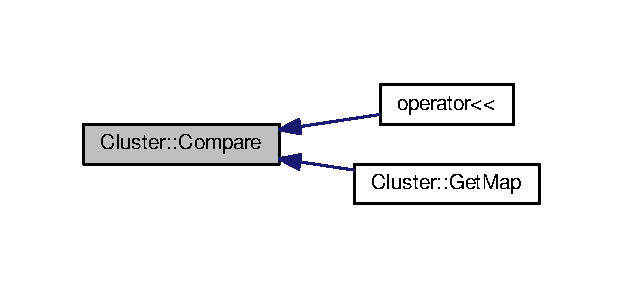
\includegraphics[width=299pt]{class_cluster_ad4f8765aefafc838c95a9c2334ee0356_icgraph}
\end{center}
\end{figure}
\mbox{\Hypertarget{class_cluster_aa890420aa5906859751f7920dc5b30d0}\label{class_cluster_aa890420aa5906859751f7920dc5b30d0}} 
\index{Cluster@{Cluster}!Get\+Cluster@{Get\+Cluster}}
\index{Get\+Cluster@{Get\+Cluster}!Cluster@{Cluster}}
\subsubsection{\texorpdfstring{Get\+Cluster()}{GetCluster()}\hspace{0.1cm}{\footnotesize\ttfamily [1/2]}}
{\footnotesize\ttfamily const vector$<$\hyperlink{class_histogram}{Histogram}$>$\& Cluster\+::\+Get\+Cluster (\begin{DoxyParamCaption}{ }\end{DoxyParamCaption}) const\hspace{0.3cm}{\ttfamily [inline]}}

Here is the caller graph for this function\+:
\nopagebreak
\begin{figure}[H]
\begin{center}
\leavevmode
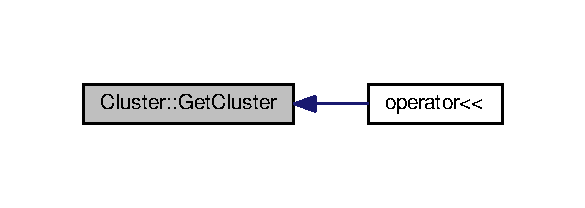
\includegraphics[width=281pt]{class_cluster_aa890420aa5906859751f7920dc5b30d0_icgraph}
\end{center}
\end{figure}
\mbox{\Hypertarget{class_cluster_a9c667ad971afdc00ffd2cb83611dabde}\label{class_cluster_a9c667ad971afdc00ffd2cb83611dabde}} 
\index{Cluster@{Cluster}!Get\+Cluster@{Get\+Cluster}}
\index{Get\+Cluster@{Get\+Cluster}!Cluster@{Cluster}}
\subsubsection{\texorpdfstring{Get\+Cluster()}{GetCluster()}\hspace{0.1cm}{\footnotesize\ttfamily [2/2]}}
{\footnotesize\ttfamily vector$<$\hyperlink{class_histogram}{Histogram}$>$\& Cluster\+::\+Get\+Cluster (\begin{DoxyParamCaption}{ }\end{DoxyParamCaption})\hspace{0.3cm}{\ttfamily [inline]}}

\mbox{\Hypertarget{class_cluster_ae703b09c81c25ab89bde18ca09aa1a5d}\label{class_cluster_ae703b09c81c25ab89bde18ca09aa1a5d}} 
\index{Cluster@{Cluster}!Get\+Exceptions@{Get\+Exceptions}}
\index{Get\+Exceptions@{Get\+Exceptions}!Cluster@{Cluster}}
\subsubsection{\texorpdfstring{Get\+Exceptions()}{GetExceptions()}}
{\footnotesize\ttfamily unordered\+\_\+map$<$string, string$>$\& Cluster\+::\+Get\+Exceptions (\begin{DoxyParamCaption}{ }\end{DoxyParamCaption})\hspace{0.3cm}{\ttfamily [inline]}}

\mbox{\Hypertarget{class_cluster_ada4f897af1294c97e3ff2f8023a92b55}\label{class_cluster_ada4f897af1294c97e3ff2f8023a92b55}} 
\index{Cluster@{Cluster}!Get\+Inverse\+Document\+Frequencies@{Get\+Inverse\+Document\+Frequencies}}
\index{Get\+Inverse\+Document\+Frequencies@{Get\+Inverse\+Document\+Frequencies}!Cluster@{Cluster}}
\subsubsection{\texorpdfstring{Get\+Inverse\+Document\+Frequencies()}{GetInverseDocumentFrequencies()}}
{\footnotesize\ttfamily map$<$ string, double $>$ Cluster\+::\+Get\+Inverse\+Document\+Frequencies (\begin{DoxyParamCaption}\item[{vector$<$ \hyperlink{class_histogram}{Histogram} $>$ \&}]{clust,  }\item[{map$<$ string, double $>$ \&}]{map }\end{DoxyParamCaption})}

Get\+Inverse\+Document\+Frequencies. Counts all instances of each string within all Histograms and stores them as a key\+\_\+value\+\_\+pair in the map returning the I\+DF of each word as a map$<$string, double$>$ Here is the caller graph for this function\+:
\nopagebreak
\begin{figure}[H]
\begin{center}
\leavevmode
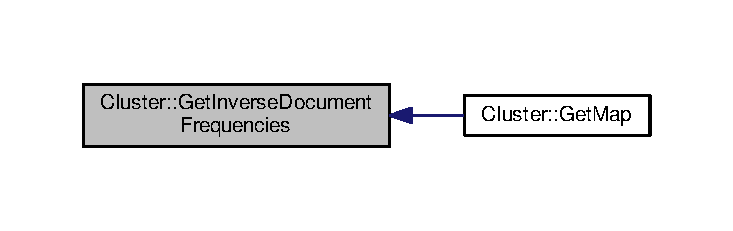
\includegraphics[width=350pt]{class_cluster_ada4f897af1294c97e3ff2f8023a92b55_icgraph}
\end{center}
\end{figure}
\mbox{\Hypertarget{class_cluster_a4e3685824bdd4b01763f8e811000f275}\label{class_cluster_a4e3685824bdd4b01763f8e811000f275}} 
\index{Cluster@{Cluster}!Get\+Map@{Get\+Map}}
\index{Get\+Map@{Get\+Map}!Cluster@{Cluster}}
\subsubsection{\texorpdfstring{Get\+Map()}{GetMap()}\hspace{0.1cm}{\footnotesize\ttfamily [1/2]}}
{\footnotesize\ttfamily const map$<$string, double$>$\& Cluster\+::\+Get\+Map (\begin{DoxyParamCaption}{ }\end{DoxyParamCaption}) const\hspace{0.3cm}{\ttfamily [inline]}}

Here is the caller graph for this function\+:
\nopagebreak
\begin{figure}[H]
\begin{center}
\leavevmode
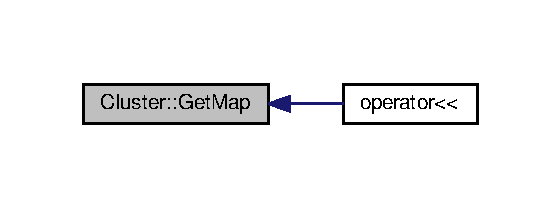
\includegraphics[width=269pt]{class_cluster_a4e3685824bdd4b01763f8e811000f275_icgraph}
\end{center}
\end{figure}
\mbox{\Hypertarget{class_cluster_a7c98f2cdd78a833e9033f8a9a5a5a7b0}\label{class_cluster_a7c98f2cdd78a833e9033f8a9a5a5a7b0}} 
\index{Cluster@{Cluster}!Get\+Map@{Get\+Map}}
\index{Get\+Map@{Get\+Map}!Cluster@{Cluster}}
\subsubsection{\texorpdfstring{Get\+Map()}{GetMap()}\hspace{0.1cm}{\footnotesize\ttfamily [2/2]}}
{\footnotesize\ttfamily map$<$string, double$>$\& Cluster\+::\+Get\+Map (\begin{DoxyParamCaption}{ }\end{DoxyParamCaption})\hspace{0.3cm}{\ttfamily [inline]}}

Here is the call graph for this function\+:
\nopagebreak
\begin{figure}[H]
\begin{center}
\leavevmode
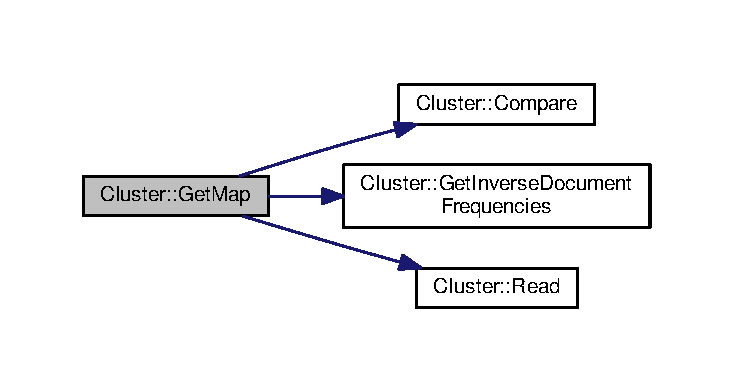
\includegraphics[width=350pt]{class_cluster_a7c98f2cdd78a833e9033f8a9a5a5a7b0_cgraph}
\end{center}
\end{figure}
\mbox{\Hypertarget{class_cluster_ad9132f66736e8f170eb7746f9cd482d0}\label{class_cluster_ad9132f66736e8f170eb7746f9cd482d0}} 
\index{Cluster@{Cluster}!Read@{Read}}
\index{Read@{Read}!Cluster@{Cluster}}
\subsubsection{\texorpdfstring{Read()}{Read()}}
{\footnotesize\ttfamily bool Cluster\+::\+Read (\begin{DoxyParamCaption}\item[{ifstream \&}]{infile,  }\item[{unordered\+\_\+map$<$ string, string $>$ \&}]{map }\end{DoxyParamCaption})}

Here is the caller graph for this function\+:
\nopagebreak
\begin{figure}[H]
\begin{center}
\leavevmode
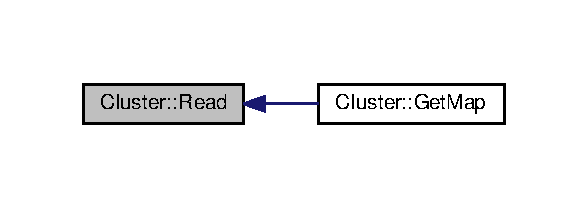
\includegraphics[width=282pt]{class_cluster_ad9132f66736e8f170eb7746f9cd482d0_icgraph}
\end{center}
\end{figure}
\mbox{\Hypertarget{class_cluster_a916e731be9d3e52a404152e94b8b127d}\label{class_cluster_a916e731be9d3e52a404152e94b8b127d}} 
\index{Cluster@{Cluster}!Size@{Size}}
\index{Size@{Size}!Cluster@{Cluster}}
\subsubsection{\texorpdfstring{Size()}{Size()}}
{\footnotesize\ttfamily unsigned int Cluster\+::\+Size (\begin{DoxyParamCaption}{ }\end{DoxyParamCaption}) const\hspace{0.3cm}{\ttfamily [inline]}}

Here is the caller graph for this function\+:
\nopagebreak
\begin{figure}[H]
\begin{center}
\leavevmode
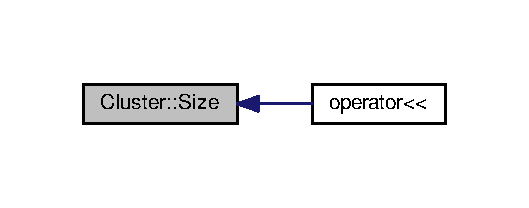
\includegraphics[width=254pt]{class_cluster_a916e731be9d3e52a404152e94b8b127d_icgraph}
\end{center}
\end{figure}


\subsection{Friends And Related Function Documentation}
\mbox{\Hypertarget{class_cluster_a80e9d0c8af3d3700176af496cc2dcf29}\label{class_cluster_a80e9d0c8af3d3700176af496cc2dcf29}} 
\index{Cluster@{Cluster}!operator$<$$<$@{operator$<$$<$}}
\index{operator$<$$<$@{operator$<$$<$}!Cluster@{Cluster}}
\subsubsection{\texorpdfstring{operator$<$$<$}{operator<<}}
{\footnotesize\ttfamily std\+::ostream\& operator$<$$<$ (\begin{DoxyParamCaption}\item[{std\+::ostream \&}]{out,  }\item[{const \hyperlink{class_cluster}{Cluster} \&}]{c0 }\end{DoxyParamCaption})\hspace{0.3cm}{\ttfamily [friend]}}



The documentation for this class was generated from the following files\+:\begin{DoxyCompactItemize}
\item 
\hyperlink{_cluster_8h}{Cluster.\+h}\item 
\hyperlink{_cluster_8cpp}{Cluster.\+cpp}\end{DoxyCompactItemize}

\hypertarget{class_coleman_liau}{}\section{Coleman\+Liau Class Reference}
\label{class_coleman_liau}\index{Coleman\+Liau@{Coleman\+Liau}}


An implementation of the Coleman-\/\+Liau index algorithm.  




{\ttfamily \#include $<$Coleman\+Liau.\+h$>$}

\subsection*{Public Member Functions}
\begin{DoxyCompactItemize}
\item 
\hyperlink{class_coleman_liau_a4ff77aa5f5ff81d167a8cabad71e620f}{Coleman\+Liau} ()
\begin{DoxyCompactList}\small\item\em Constructor. \end{DoxyCompactList}\item 
\hyperlink{class_coleman_liau_a0b46f263a2dd687c2fa89bbef88002d0}{Coleman\+Liau} (double index)
\item 
double \hyperlink{class_coleman_liau_a3a9e5cb64586313a753211c350147cb3}{get\+Index} ()
\item 
bool \hyperlink{class_coleman_liau_af0b2de26e53db82cb3e7243de1f26a6f}{Eval} (\hyperlink{class_histogram}{Histogram} \&Hist)
\item 
void \hyperlink{class_coleman_liau_a077d1533dfd8145ed729531c6edbfad0}{set\+Index} (double index)
\end{DoxyCompactItemize}
\subsection*{Friends}
\begin{DoxyCompactItemize}
\item 
std\+::ostream \& \hyperlink{class_coleman_liau_a896867aacd954df4faecc74a7010a8b0}{operator$<$$<$} (std\+::ostream \&out, const \hyperlink{class_coleman_liau}{Coleman\+Liau} \&c0)
\end{DoxyCompactItemize}


\subsection{Detailed Description}
An implementation of the Coleman-\/\+Liau index algorithm. 

A class for determining the reading level of a given histogram (document) 

\subsection{Constructor \& Destructor Documentation}
\mbox{\Hypertarget{class_coleman_liau_a4ff77aa5f5ff81d167a8cabad71e620f}\label{class_coleman_liau_a4ff77aa5f5ff81d167a8cabad71e620f}} 
\index{Coleman\+Liau@{Coleman\+Liau}!Coleman\+Liau@{Coleman\+Liau}}
\index{Coleman\+Liau@{Coleman\+Liau}!Coleman\+Liau@{Coleman\+Liau}}
\subsubsection{\texorpdfstring{Coleman\+Liau()}{ColemanLiau()}\hspace{0.1cm}{\footnotesize\ttfamily [1/2]}}
{\footnotesize\ttfamily Coleman\+Liau\+::\+Coleman\+Liau (\begin{DoxyParamCaption}{ }\end{DoxyParamCaption})\hspace{0.3cm}{\ttfamily [inline]}}



Constructor. 

\mbox{\Hypertarget{class_coleman_liau_a0b46f263a2dd687c2fa89bbef88002d0}\label{class_coleman_liau_a0b46f263a2dd687c2fa89bbef88002d0}} 
\index{Coleman\+Liau@{Coleman\+Liau}!Coleman\+Liau@{Coleman\+Liau}}
\index{Coleman\+Liau@{Coleman\+Liau}!Coleman\+Liau@{Coleman\+Liau}}
\subsubsection{\texorpdfstring{Coleman\+Liau()}{ColemanLiau()}\hspace{0.1cm}{\footnotesize\ttfamily [2/2]}}
{\footnotesize\ttfamily Coleman\+Liau\+::\+Coleman\+Liau (\begin{DoxyParamCaption}\item[{double}]{index }\end{DoxyParamCaption})\hspace{0.3cm}{\ttfamily [inline]}}



\subsection{Member Function Documentation}
\mbox{\Hypertarget{class_coleman_liau_af0b2de26e53db82cb3e7243de1f26a6f}\label{class_coleman_liau_af0b2de26e53db82cb3e7243de1f26a6f}} 
\index{Coleman\+Liau@{Coleman\+Liau}!Eval@{Eval}}
\index{Eval@{Eval}!Coleman\+Liau@{Coleman\+Liau}}
\subsubsection{\texorpdfstring{Eval()}{Eval()}}
{\footnotesize\ttfamily bool Coleman\+Liau\+::\+Eval (\begin{DoxyParamCaption}\item[{\hyperlink{class_histogram}{Histogram} \&}]{Hist }\end{DoxyParamCaption})}

Evaluation operator. Takes a \hyperlink{class_histogram}{Histogram} and applies the Coleman-\/\+Liau equation to comeup with a reading level of the document Here is the caller graph for this function\+:
\nopagebreak
\begin{figure}[H]
\begin{center}
\leavevmode
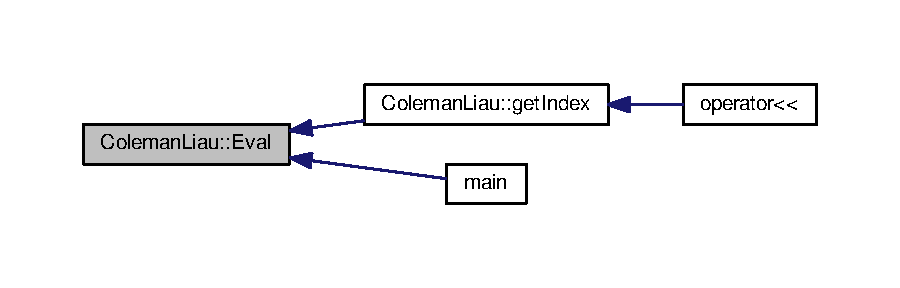
\includegraphics[width=350pt]{class_coleman_liau_af0b2de26e53db82cb3e7243de1f26a6f_icgraph}
\end{center}
\end{figure}
\mbox{\Hypertarget{class_coleman_liau_a3a9e5cb64586313a753211c350147cb3}\label{class_coleman_liau_a3a9e5cb64586313a753211c350147cb3}} 
\index{Coleman\+Liau@{Coleman\+Liau}!get\+Index@{get\+Index}}
\index{get\+Index@{get\+Index}!Coleman\+Liau@{Coleman\+Liau}}
\subsubsection{\texorpdfstring{get\+Index()}{getIndex()}}
{\footnotesize\ttfamily double Coleman\+Liau\+::get\+Index (\begin{DoxyParamCaption}{ }\end{DoxyParamCaption})\hspace{0.3cm}{\ttfamily [inline]}}

Here is the call graph for this function\+:
\nopagebreak
\begin{figure}[H]
\begin{center}
\leavevmode
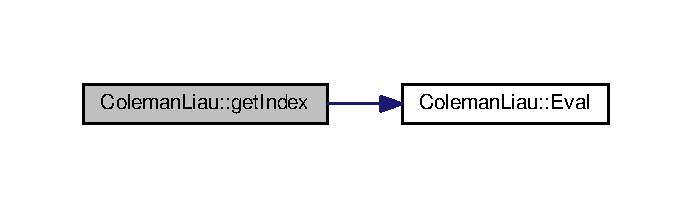
\includegraphics[width=332pt]{class_coleman_liau_a3a9e5cb64586313a753211c350147cb3_cgraph}
\end{center}
\end{figure}
Here is the caller graph for this function\+:
\nopagebreak
\begin{figure}[H]
\begin{center}
\leavevmode
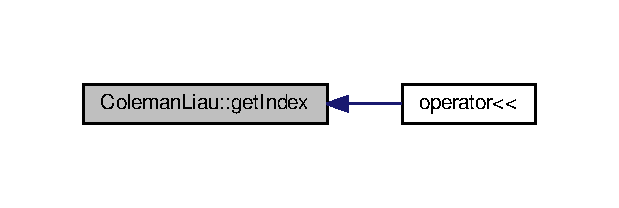
\includegraphics[width=297pt]{class_coleman_liau_a3a9e5cb64586313a753211c350147cb3_icgraph}
\end{center}
\end{figure}
\mbox{\Hypertarget{class_coleman_liau_a077d1533dfd8145ed729531c6edbfad0}\label{class_coleman_liau_a077d1533dfd8145ed729531c6edbfad0}} 
\index{Coleman\+Liau@{Coleman\+Liau}!set\+Index@{set\+Index}}
\index{set\+Index@{set\+Index}!Coleman\+Liau@{Coleman\+Liau}}
\subsubsection{\texorpdfstring{set\+Index()}{setIndex()}}
{\footnotesize\ttfamily void Coleman\+Liau\+::set\+Index (\begin{DoxyParamCaption}\item[{double}]{index }\end{DoxyParamCaption})\hspace{0.3cm}{\ttfamily [inline]}}



\subsection{Friends And Related Function Documentation}
\mbox{\Hypertarget{class_coleman_liau_a896867aacd954df4faecc74a7010a8b0}\label{class_coleman_liau_a896867aacd954df4faecc74a7010a8b0}} 
\index{Coleman\+Liau@{Coleman\+Liau}!operator$<$$<$@{operator$<$$<$}}
\index{operator$<$$<$@{operator$<$$<$}!Coleman\+Liau@{Coleman\+Liau}}
\subsubsection{\texorpdfstring{operator$<$$<$}{operator<<}}
{\footnotesize\ttfamily std\+::ostream\& operator$<$$<$ (\begin{DoxyParamCaption}\item[{std\+::ostream \&}]{out,  }\item[{const \hyperlink{class_coleman_liau}{Coleman\+Liau} \&}]{c0 }\end{DoxyParamCaption})\hspace{0.3cm}{\ttfamily [friend]}}



The documentation for this class was generated from the following files\+:\begin{DoxyCompactItemize}
\item 
\hyperlink{_coleman_liau_8h}{Coleman\+Liau.\+h}\item 
\hyperlink{_coleman_liau_8cpp}{Coleman\+Liau.\+cpp}\end{DoxyCompactItemize}

\hypertarget{class_histogram}{}\section{Histogram Class Reference}
\label{class_histogram}\index{Histogram@{Histogram}}


A string histogram for simple counting (currently)  




{\ttfamily \#include $<$Histogram.\+h$>$}

\subsection*{Public Member Functions}
\begin{DoxyCompactItemize}
\item 
\hyperlink{class_histogram_af681f293852ac145f867ecfcce3062a5}{Histogram} ()
\begin{DoxyCompactList}\small\item\em Constructor. \end{DoxyCompactList}\item 
\hyperlink{class_histogram_a5e56d61b85862889a024c1a682981964}{Histogram} (vector$<$ \hyperlink{class_lexeme}{Lexeme} $>$ h)
\item 
vector$<$ \hyperlink{class_lexeme}{Lexeme} $>$ \& \hyperlink{class_histogram_afe807b7c5109c6a9781216961f2a9e90}{Get\+Hist} ()
\item 
const map$<$ string, int $>$ \& \hyperlink{class_histogram_a605a2f87dcbe0c52e956ed6e559daf81}{Get\+Map} () const
\item 
bool \hyperlink{class_histogram_aff24f16064c037ca8929c4f9751aedbf}{is\+Exception} (const string \&str, const unsigned int i) const
\item 
bool \hyperlink{class_histogram_af8b644d9dcb8dd86fb3420640de72ab2}{Write} (ostream \&ostr, map$<$ string, int $>$ \&kvm) const
\item 
map$<$ string, int $>$ \& \hyperlink{class_histogram_a7a4b270eb5d88df6466cef9433a95d39}{Get\+Map} ()
\item 
void \hyperlink{class_histogram_a3b48f22da2e0c9f1d12ecd7a83f0dcf6}{Set\+String} (const string new\+Value, const int position)
\item 
void \hyperlink{class_histogram_af4fdfc3e8e4c4028deaf9b663ee5832c}{Eval} ()
\item 
bool \hyperlink{class_histogram_afbdf1d9a97070fd3724dbe55fd9f8570}{Read} (istream \&istr, vector$<$ \hyperlink{class_lexeme}{Lexeme} $>$ \&histogram)
\item 
string \hyperlink{class_histogram_aa1ae3a4f490aef85530afc028867b8f4}{parse\+Punctuation} (string word, vector$<$ \hyperlink{class_lexeme}{Lexeme} $>$ \&histogram)
\item 
void \hyperlink{class_histogram_a97384bc67a4fcbd79f405329de0a4b41}{find\+Capitals} (vector$<$ \hyperlink{class_lexeme}{Lexeme} $>$ \&histogram)
\item 
void \hyperlink{class_histogram_a5adb0e9b69168b662af9f84cbf29d5a0}{resolve\+Ambiguity} (vector$<$ \hyperlink{class_lexeme}{Lexeme} $>$ \&histogram)
\end{DoxyCompactItemize}


\subsection{Detailed Description}
A string histogram for simple counting (currently) 

A class for counting the instances of strings from a file. This class currently does nothing more than count totals and output said counts to the console. 

\subsection{Constructor \& Destructor Documentation}
\mbox{\Hypertarget{class_histogram_af681f293852ac145f867ecfcce3062a5}\label{class_histogram_af681f293852ac145f867ecfcce3062a5}} 
\index{Histogram@{Histogram}!Histogram@{Histogram}}
\index{Histogram@{Histogram}!Histogram@{Histogram}}
\subsubsection{\texorpdfstring{Histogram()}{Histogram()}\hspace{0.1cm}{\footnotesize\ttfamily [1/2]}}
{\footnotesize\ttfamily Histogram\+::\+Histogram (\begin{DoxyParamCaption}{ }\end{DoxyParamCaption})\hspace{0.3cm}{\ttfamily [inline]}}



Constructor. 

\mbox{\Hypertarget{class_histogram_a5e56d61b85862889a024c1a682981964}\label{class_histogram_a5e56d61b85862889a024c1a682981964}} 
\index{Histogram@{Histogram}!Histogram@{Histogram}}
\index{Histogram@{Histogram}!Histogram@{Histogram}}
\subsubsection{\texorpdfstring{Histogram()}{Histogram()}\hspace{0.1cm}{\footnotesize\ttfamily [2/2]}}
{\footnotesize\ttfamily Histogram\+::\+Histogram (\begin{DoxyParamCaption}\item[{vector$<$ \hyperlink{class_lexeme}{Lexeme} $>$}]{h }\end{DoxyParamCaption})\hspace{0.3cm}{\ttfamily [inline]}}



\subsection{Member Function Documentation}
\mbox{\Hypertarget{class_histogram_af4fdfc3e8e4c4028deaf9b663ee5832c}\label{class_histogram_af4fdfc3e8e4c4028deaf9b663ee5832c}} 
\index{Histogram@{Histogram}!Eval@{Eval}}
\index{Eval@{Eval}!Histogram@{Histogram}}
\subsubsection{\texorpdfstring{Eval()}{Eval()}}
{\footnotesize\ttfamily void Histogram\+::\+Eval (\begin{DoxyParamCaption}{ }\end{DoxyParamCaption})}

Evaluation operator. Counts all instances of distinct strings within the histogram and stores them as a key\+\_\+value\+\_\+pair in the map Here is the caller graph for this function\+:
\nopagebreak
\begin{figure}[H]
\begin{center}
\leavevmode
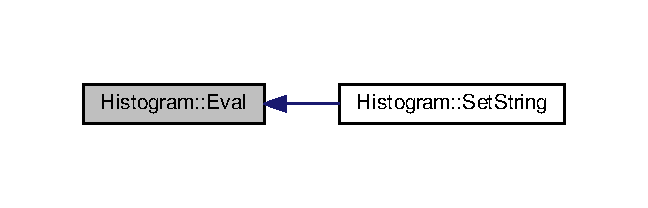
\includegraphics[width=311pt]{class_histogram_af4fdfc3e8e4c4028deaf9b663ee5832c_icgraph}
\end{center}
\end{figure}
\mbox{\Hypertarget{class_histogram_a97384bc67a4fcbd79f405329de0a4b41}\label{class_histogram_a97384bc67a4fcbd79f405329de0a4b41}} 
\index{Histogram@{Histogram}!find\+Capitals@{find\+Capitals}}
\index{find\+Capitals@{find\+Capitals}!Histogram@{Histogram}}
\subsubsection{\texorpdfstring{find\+Capitals()}{findCapitals()}}
{\footnotesize\ttfamily void Histogram\+::find\+Capitals (\begin{DoxyParamCaption}\item[{vector$<$ \hyperlink{class_lexeme}{Lexeme} $>$ \&}]{histogram }\end{DoxyParamCaption})}

Here is the call graph for this function\+:
\nopagebreak
\begin{figure}[H]
\begin{center}
\leavevmode
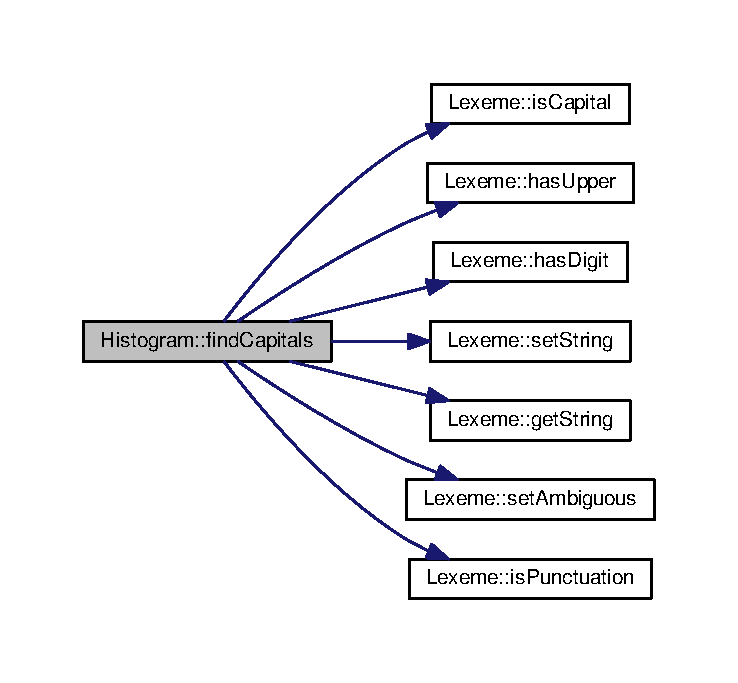
\includegraphics[width=350pt]{class_histogram_a97384bc67a4fcbd79f405329de0a4b41_cgraph}
\end{center}
\end{figure}
Here is the caller graph for this function\+:
\nopagebreak
\begin{figure}[H]
\begin{center}
\leavevmode
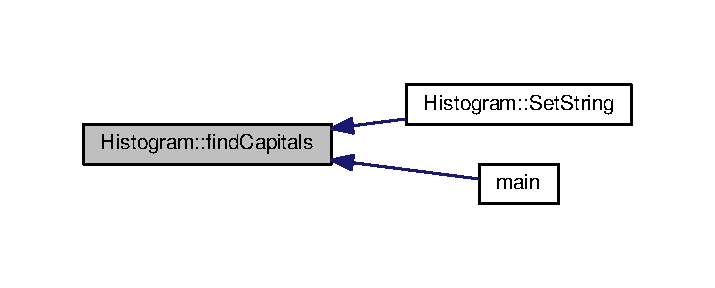
\includegraphics[width=343pt]{class_histogram_a97384bc67a4fcbd79f405329de0a4b41_icgraph}
\end{center}
\end{figure}
\mbox{\Hypertarget{class_histogram_afe807b7c5109c6a9781216961f2a9e90}\label{class_histogram_afe807b7c5109c6a9781216961f2a9e90}} 
\index{Histogram@{Histogram}!Get\+Hist@{Get\+Hist}}
\index{Get\+Hist@{Get\+Hist}!Histogram@{Histogram}}
\subsubsection{\texorpdfstring{Get\+Hist()}{GetHist()}}
{\footnotesize\ttfamily vector$<$\hyperlink{class_lexeme}{Lexeme}$>$\& Histogram\+::\+Get\+Hist (\begin{DoxyParamCaption}{ }\end{DoxyParamCaption})\hspace{0.3cm}{\ttfamily [inline]}}

Here is the caller graph for this function\+:
\nopagebreak
\begin{figure}[H]
\begin{center}
\leavevmode
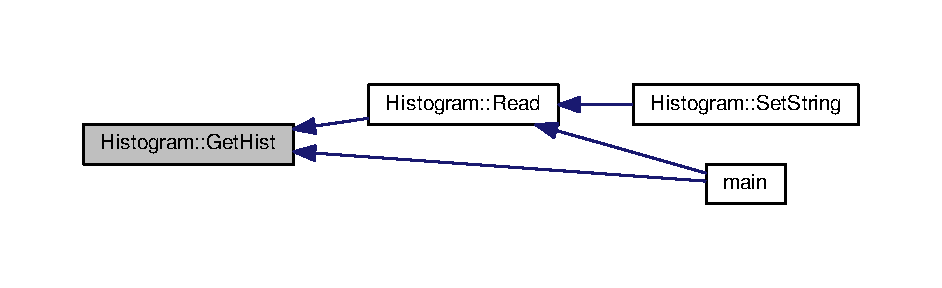
\includegraphics[width=350pt]{class_histogram_afe807b7c5109c6a9781216961f2a9e90_icgraph}
\end{center}
\end{figure}
\mbox{\Hypertarget{class_histogram_a605a2f87dcbe0c52e956ed6e559daf81}\label{class_histogram_a605a2f87dcbe0c52e956ed6e559daf81}} 
\index{Histogram@{Histogram}!Get\+Map@{Get\+Map}}
\index{Get\+Map@{Get\+Map}!Histogram@{Histogram}}
\subsubsection{\texorpdfstring{Get\+Map()}{GetMap()}\hspace{0.1cm}{\footnotesize\ttfamily [1/2]}}
{\footnotesize\ttfamily const map$<$string, int$>$\& Histogram\+::\+Get\+Map (\begin{DoxyParamCaption}{ }\end{DoxyParamCaption}) const\hspace{0.3cm}{\ttfamily [inline]}}

Here is the call graph for this function\+:
\nopagebreak
\begin{figure}[H]
\begin{center}
\leavevmode
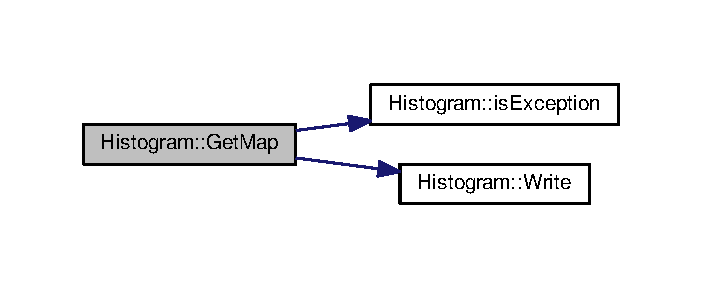
\includegraphics[width=337pt]{class_histogram_a605a2f87dcbe0c52e956ed6e559daf81_cgraph}
\end{center}
\end{figure}
\mbox{\Hypertarget{class_histogram_a7a4b270eb5d88df6466cef9433a95d39}\label{class_histogram_a7a4b270eb5d88df6466cef9433a95d39}} 
\index{Histogram@{Histogram}!Get\+Map@{Get\+Map}}
\index{Get\+Map@{Get\+Map}!Histogram@{Histogram}}
\subsubsection{\texorpdfstring{Get\+Map()}{GetMap()}\hspace{0.1cm}{\footnotesize\ttfamily [2/2]}}
{\footnotesize\ttfamily map$<$string, int$>$\& Histogram\+::\+Get\+Map (\begin{DoxyParamCaption}{ }\end{DoxyParamCaption})\hspace{0.3cm}{\ttfamily [inline]}}

\mbox{\Hypertarget{class_histogram_aff24f16064c037ca8929c4f9751aedbf}\label{class_histogram_aff24f16064c037ca8929c4f9751aedbf}} 
\index{Histogram@{Histogram}!is\+Exception@{is\+Exception}}
\index{is\+Exception@{is\+Exception}!Histogram@{Histogram}}
\subsubsection{\texorpdfstring{is\+Exception()}{isException()}}
{\footnotesize\ttfamily bool Histogram\+::is\+Exception (\begin{DoxyParamCaption}\item[{const string \&}]{word,  }\item[{const unsigned int}]{i }\end{DoxyParamCaption}) const}

Is this character an exception to the punctuation checks the string against the provided exceptoins to ensure that it is valid int i = the location in the word (to en Here is the caller graph for this function\+:
\nopagebreak
\begin{figure}[H]
\begin{center}
\leavevmode
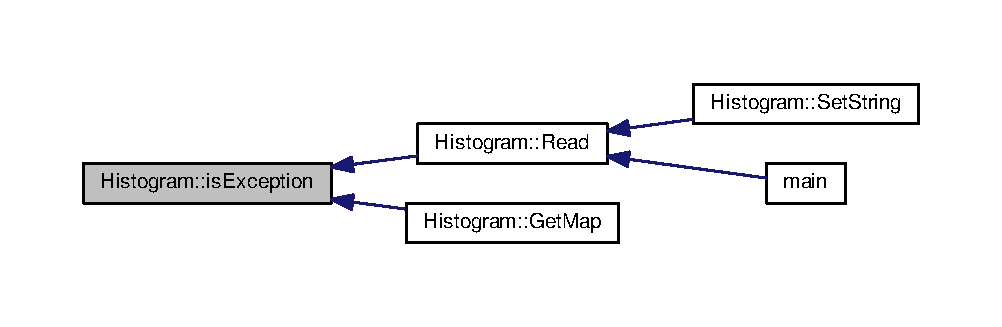
\includegraphics[width=350pt]{class_histogram_aff24f16064c037ca8929c4f9751aedbf_icgraph}
\end{center}
\end{figure}
\mbox{\Hypertarget{class_histogram_aa1ae3a4f490aef85530afc028867b8f4}\label{class_histogram_aa1ae3a4f490aef85530afc028867b8f4}} 
\index{Histogram@{Histogram}!parse\+Punctuation@{parse\+Punctuation}}
\index{parse\+Punctuation@{parse\+Punctuation}!Histogram@{Histogram}}
\subsubsection{\texorpdfstring{parse\+Punctuation()}{parsePunctuation()}}
{\footnotesize\ttfamily string Histogram\+::parse\+Punctuation (\begin{DoxyParamCaption}\item[{string}]{word,  }\item[{vector$<$ \hyperlink{class_lexeme}{Lexeme} $>$ \&}]{hist }\end{DoxyParamCaption})}

Parse Punctuation. Takes a string and a vector$<$\+Lexeme$>$\& searches the str and parses out any punctuation returns a string such that ispunct(str\mbox{[}0\mbox{]}) = F\+A\+L\+SE Here is the caller graph for this function\+:
\nopagebreak
\begin{figure}[H]
\begin{center}
\leavevmode
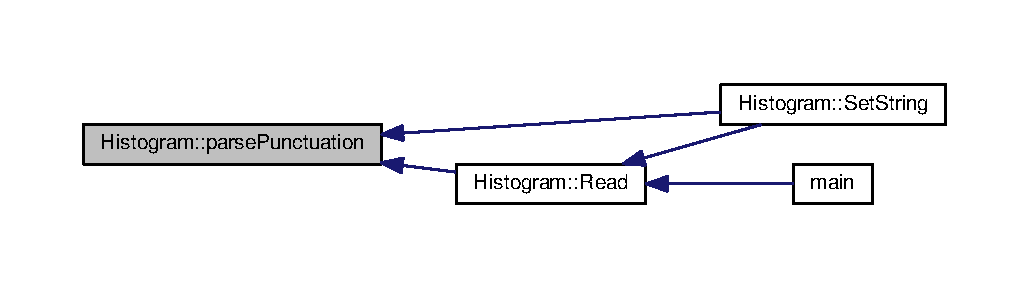
\includegraphics[width=350pt]{class_histogram_aa1ae3a4f490aef85530afc028867b8f4_icgraph}
\end{center}
\end{figure}
\mbox{\Hypertarget{class_histogram_afbdf1d9a97070fd3724dbe55fd9f8570}\label{class_histogram_afbdf1d9a97070fd3724dbe55fd9f8570}} 
\index{Histogram@{Histogram}!Read@{Read}}
\index{Read@{Read}!Histogram@{Histogram}}
\subsubsection{\texorpdfstring{Read()}{Read()}}
{\footnotesize\ttfamily bool Histogram\+::\+Read (\begin{DoxyParamCaption}\item[{istream \&}]{istr,  }\item[{vector$<$ \hyperlink{class_lexeme}{Lexeme} $>$ \&}]{hist }\end{DoxyParamCaption})}

Input operator. Format is string string ... str, where all strings are delineated by whitespace. Any other format causes the input stream to fail. Here is the call graph for this function\+:
\nopagebreak
\begin{figure}[H]
\begin{center}
\leavevmode
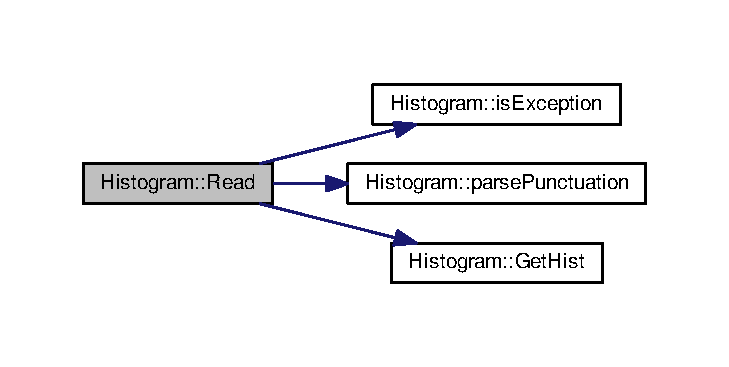
\includegraphics[width=350pt]{class_histogram_afbdf1d9a97070fd3724dbe55fd9f8570_cgraph}
\end{center}
\end{figure}
Here is the caller graph for this function\+:
\nopagebreak
\begin{figure}[H]
\begin{center}
\leavevmode
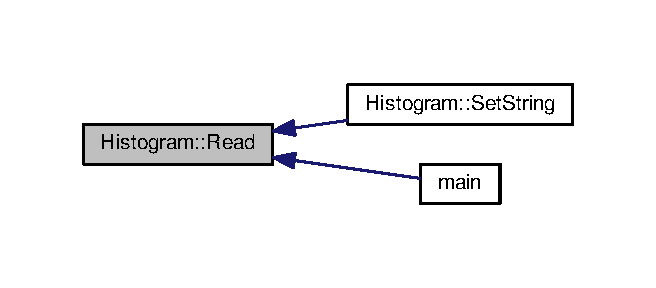
\includegraphics[width=315pt]{class_histogram_afbdf1d9a97070fd3724dbe55fd9f8570_icgraph}
\end{center}
\end{figure}
\mbox{\Hypertarget{class_histogram_a5adb0e9b69168b662af9f84cbf29d5a0}\label{class_histogram_a5adb0e9b69168b662af9f84cbf29d5a0}} 
\index{Histogram@{Histogram}!resolve\+Ambiguity@{resolve\+Ambiguity}}
\index{resolve\+Ambiguity@{resolve\+Ambiguity}!Histogram@{Histogram}}
\subsubsection{\texorpdfstring{resolve\+Ambiguity()}{resolveAmbiguity()}}
{\footnotesize\ttfamily void Histogram\+::resolve\+Ambiguity (\begin{DoxyParamCaption}\item[{vector$<$ \hyperlink{class_lexeme}{Lexeme} $>$ \&}]{hist }\end{DoxyParamCaption})}

Is this string supposed to be a capital or not this method will check to see if we find any other instance of the ambiguous word in the rest of the document if so ? leave capital \+: make it lowercase Here is the caller graph for this function\+:
\nopagebreak
\begin{figure}[H]
\begin{center}
\leavevmode
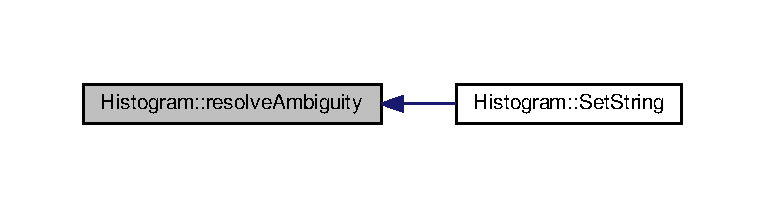
\includegraphics[width=350pt]{class_histogram_a5adb0e9b69168b662af9f84cbf29d5a0_icgraph}
\end{center}
\end{figure}
\mbox{\Hypertarget{class_histogram_a3b48f22da2e0c9f1d12ecd7a83f0dcf6}\label{class_histogram_a3b48f22da2e0c9f1d12ecd7a83f0dcf6}} 
\index{Histogram@{Histogram}!Set\+String@{Set\+String}}
\index{Set\+String@{Set\+String}!Histogram@{Histogram}}
\subsubsection{\texorpdfstring{Set\+String()}{SetString()}}
{\footnotesize\ttfamily void Histogram\+::\+Set\+String (\begin{DoxyParamCaption}\item[{const string}]{new\+Value,  }\item[{const int}]{position }\end{DoxyParamCaption})\hspace{0.3cm}{\ttfamily [inline]}}

Here is the call graph for this function\+:
\nopagebreak
\begin{figure}[H]
\begin{center}
\leavevmode
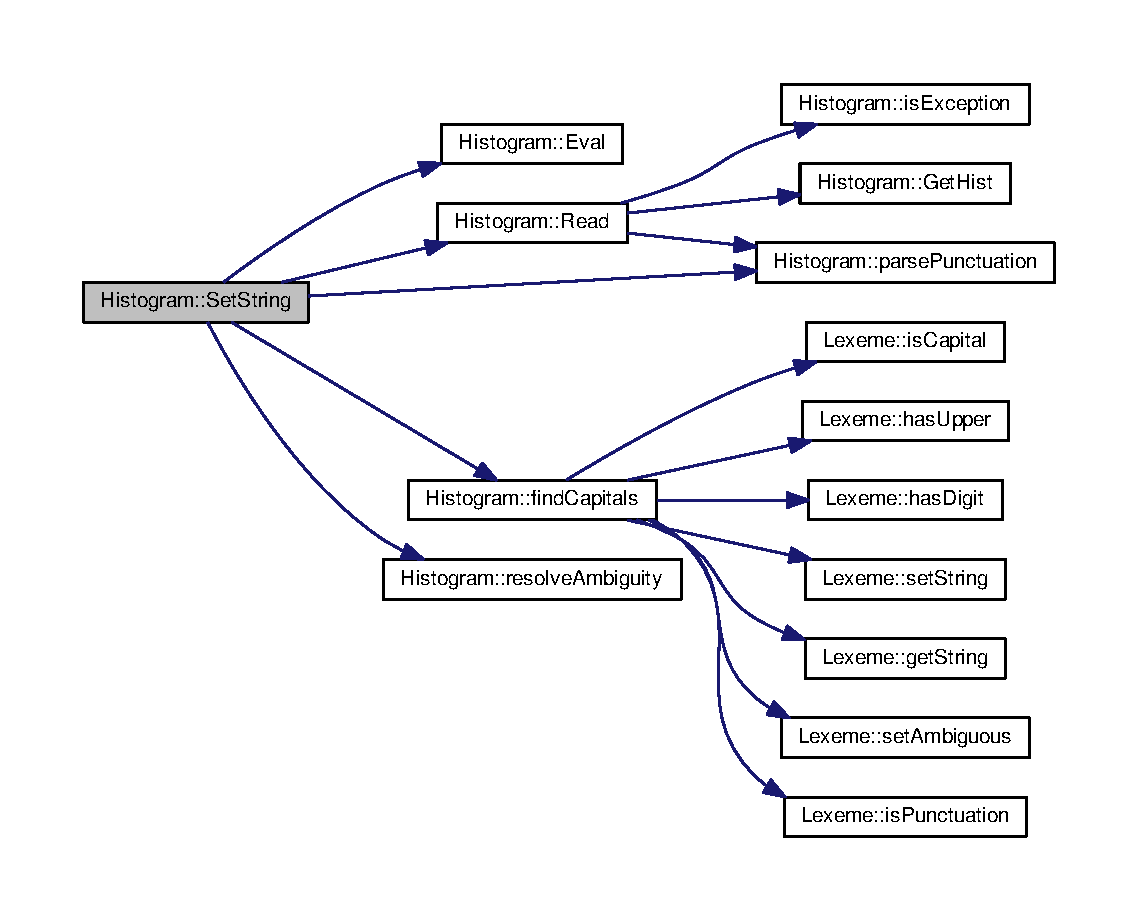
\includegraphics[width=350pt]{class_histogram_a3b48f22da2e0c9f1d12ecd7a83f0dcf6_cgraph}
\end{center}
\end{figure}
\mbox{\Hypertarget{class_histogram_af8b644d9dcb8dd86fb3420640de72ab2}\label{class_histogram_af8b644d9dcb8dd86fb3420640de72ab2}} 
\index{Histogram@{Histogram}!Write@{Write}}
\index{Write@{Write}!Histogram@{Histogram}}
\subsubsection{\texorpdfstring{Write()}{Write()}}
{\footnotesize\ttfamily bool Histogram\+::\+Write (\begin{DoxyParamCaption}\item[{ostream \&}]{ostr,  }\item[{map$<$ string, int $>$ \&}]{kvm }\end{DoxyParamCaption}) const}

Write operator. Typical output operator. Takes an ostream\& and a map$<$string, int$>$ dumps the key\+\_\+value\+\_\+pairs to the ostream provided Erros on an empty map$<$string, int$>$ Here is the caller graph for this function\+:
\nopagebreak
\begin{figure}[H]
\begin{center}
\leavevmode
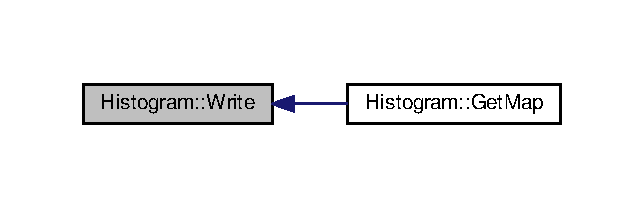
\includegraphics[width=309pt]{class_histogram_af8b644d9dcb8dd86fb3420640de72ab2_icgraph}
\end{center}
\end{figure}


The documentation for this class was generated from the following files\+:\begin{DoxyCompactItemize}
\item 
\hyperlink{_histogram_8h}{Histogram.\+h}\item 
\hyperlink{_histogram_8cpp}{Histogram.\+cpp}\end{DoxyCompactItemize}

\hypertarget{class_lexeme}{}\section{Lexeme Class Reference}
\label{class_lexeme}\index{Lexeme@{Lexeme}}


An implementation of a lexeme (word)  




{\ttfamily \#include $<$Lexeme.\+h$>$}

\subsection*{Public Member Functions}
\begin{DoxyCompactItemize}
\item 
\hyperlink{class_lexeme_a91ec217d9cc9c11b33597705b1f2ef88}{Lexeme} (string s=\char`\"{}\char`\"{}, bool c=0, int p=0, bool d=0, bool u=0, bool a=0)
\begin{DoxyCompactList}\small\item\em Constructor. \end{DoxyCompactList}\item 
bool \hyperlink{class_lexeme_a01b2154c183663f7e298b564d14a907e}{has\+Digit} () const
\item 
bool \hyperlink{class_lexeme_a5b40ad2f0863cbae11b0dd2c7876d8e8}{has\+Upper} () const
\item 
bool \hyperlink{class_lexeme_a6319c062333968f1d47f69d7fd44900c}{is\+Ambiguous} () const
\item 
bool \hyperlink{class_lexeme_afa5bf60e2cd601b4755cc137c56f7aed}{is\+Capital} () const
\item 
int \hyperlink{class_lexeme_a67fb5732247889cb97612dd327c7a194}{is\+Punctuation} () const
\item 
string \& \hyperlink{class_lexeme_ac3bedb54fb40b5b7d85edb3cf2d715db}{get\+String} ()
\item 
void \hyperlink{class_lexeme_a8fd310c078c13d53dc601c299d0acb78}{set\+Ambiguous} (bool amb)
\item 
void \hyperlink{class_lexeme_aa54d86594141f95df8a0364aebc931f2}{set\+Capital} (bool cap)
\item 
void \hyperlink{class_lexeme_a4bf15e88113bc3cd10dff188fef37752}{set\+Digit} (bool digi)
\item 
void \hyperlink{class_lexeme_a620288e33ed2b3957023b3d325febc13}{set\+Punctuation} (int punct)
\item 
void \hyperlink{class_lexeme_a90a1a2080fb503b0a206a075fd4d038a}{set\+String} (string s)
\item 
void \hyperlink{class_lexeme_a09873449eb90bc9be0f4df1edcf97b26}{set\+Upper} (bool up)
\end{DoxyCompactItemize}


\subsection{Detailed Description}
An implementation of a lexeme (word) 

A class for holding a word along with some key attributes that are needed to compute the stem and some other things 

\subsection{Constructor \& Destructor Documentation}
\mbox{\Hypertarget{class_lexeme_a91ec217d9cc9c11b33597705b1f2ef88}\label{class_lexeme_a91ec217d9cc9c11b33597705b1f2ef88}} 
\index{Lexeme@{Lexeme}!Lexeme@{Lexeme}}
\index{Lexeme@{Lexeme}!Lexeme@{Lexeme}}
\subsubsection{\texorpdfstring{Lexeme()}{Lexeme()}}
{\footnotesize\ttfamily Lexeme\+::\+Lexeme (\begin{DoxyParamCaption}\item[{string}]{s = {\ttfamily \char`\"{}\char`\"{}},  }\item[{bool}]{c = {\ttfamily 0},  }\item[{int}]{p = {\ttfamily 0},  }\item[{bool}]{d = {\ttfamily 0},  }\item[{bool}]{u = {\ttfamily 0},  }\item[{bool}]{a = {\ttfamily 0} }\end{DoxyParamCaption})\hspace{0.3cm}{\ttfamily [inline]}}



Constructor. 



\subsection{Member Function Documentation}
\mbox{\Hypertarget{class_lexeme_ac3bedb54fb40b5b7d85edb3cf2d715db}\label{class_lexeme_ac3bedb54fb40b5b7d85edb3cf2d715db}} 
\index{Lexeme@{Lexeme}!get\+String@{get\+String}}
\index{get\+String@{get\+String}!Lexeme@{Lexeme}}
\subsubsection{\texorpdfstring{get\+String()}{getString()}}
{\footnotesize\ttfamily string\& Lexeme\+::get\+String (\begin{DoxyParamCaption}{ }\end{DoxyParamCaption})\hspace{0.3cm}{\ttfamily [inline]}}

Here is the caller graph for this function\+:
\nopagebreak
\begin{figure}[H]
\begin{center}
\leavevmode
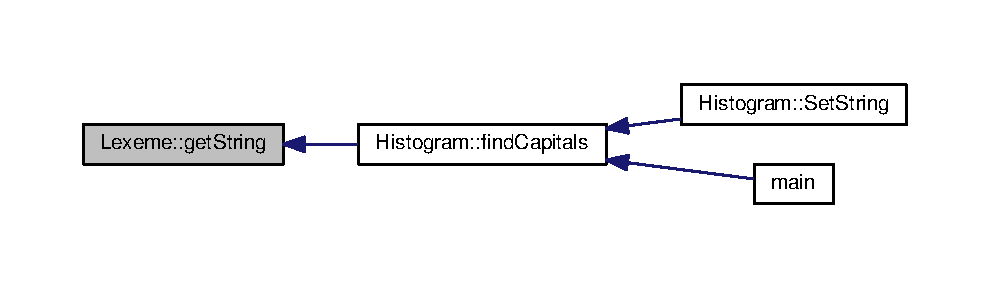
\includegraphics[width=350pt]{class_lexeme_ac3bedb54fb40b5b7d85edb3cf2d715db_icgraph}
\end{center}
\end{figure}
\mbox{\Hypertarget{class_lexeme_a01b2154c183663f7e298b564d14a907e}\label{class_lexeme_a01b2154c183663f7e298b564d14a907e}} 
\index{Lexeme@{Lexeme}!has\+Digit@{has\+Digit}}
\index{has\+Digit@{has\+Digit}!Lexeme@{Lexeme}}
\subsubsection{\texorpdfstring{has\+Digit()}{hasDigit()}}
{\footnotesize\ttfamily bool Lexeme\+::has\+Digit (\begin{DoxyParamCaption}{ }\end{DoxyParamCaption}) const\hspace{0.3cm}{\ttfamily [inline]}}

Here is the caller graph for this function\+:
\nopagebreak
\begin{figure}[H]
\begin{center}
\leavevmode
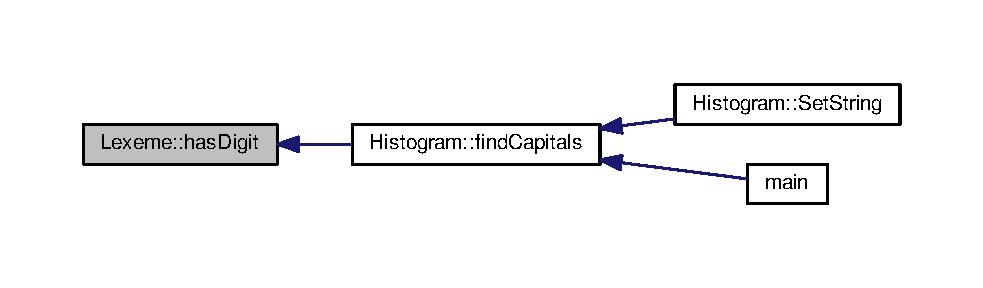
\includegraphics[width=350pt]{class_lexeme_a01b2154c183663f7e298b564d14a907e_icgraph}
\end{center}
\end{figure}
\mbox{\Hypertarget{class_lexeme_a5b40ad2f0863cbae11b0dd2c7876d8e8}\label{class_lexeme_a5b40ad2f0863cbae11b0dd2c7876d8e8}} 
\index{Lexeme@{Lexeme}!has\+Upper@{has\+Upper}}
\index{has\+Upper@{has\+Upper}!Lexeme@{Lexeme}}
\subsubsection{\texorpdfstring{has\+Upper()}{hasUpper()}}
{\footnotesize\ttfamily bool Lexeme\+::has\+Upper (\begin{DoxyParamCaption}{ }\end{DoxyParamCaption}) const\hspace{0.3cm}{\ttfamily [inline]}}

Here is the caller graph for this function\+:
\nopagebreak
\begin{figure}[H]
\begin{center}
\leavevmode
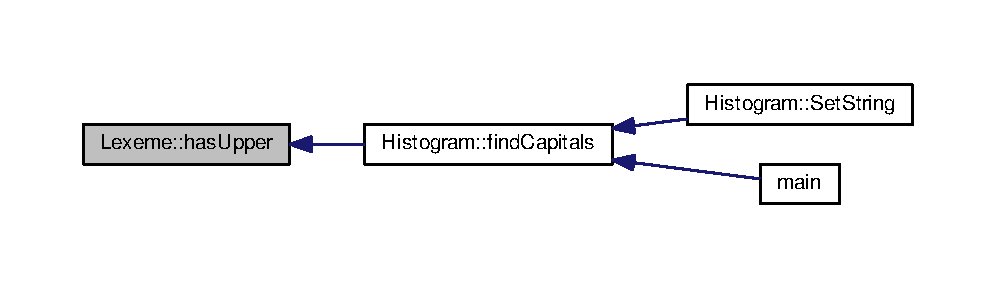
\includegraphics[width=350pt]{class_lexeme_a5b40ad2f0863cbae11b0dd2c7876d8e8_icgraph}
\end{center}
\end{figure}
\mbox{\Hypertarget{class_lexeme_a6319c062333968f1d47f69d7fd44900c}\label{class_lexeme_a6319c062333968f1d47f69d7fd44900c}} 
\index{Lexeme@{Lexeme}!is\+Ambiguous@{is\+Ambiguous}}
\index{is\+Ambiguous@{is\+Ambiguous}!Lexeme@{Lexeme}}
\subsubsection{\texorpdfstring{is\+Ambiguous()}{isAmbiguous()}}
{\footnotesize\ttfamily bool Lexeme\+::is\+Ambiguous (\begin{DoxyParamCaption}{ }\end{DoxyParamCaption}) const\hspace{0.3cm}{\ttfamily [inline]}}

\mbox{\Hypertarget{class_lexeme_afa5bf60e2cd601b4755cc137c56f7aed}\label{class_lexeme_afa5bf60e2cd601b4755cc137c56f7aed}} 
\index{Lexeme@{Lexeme}!is\+Capital@{is\+Capital}}
\index{is\+Capital@{is\+Capital}!Lexeme@{Lexeme}}
\subsubsection{\texorpdfstring{is\+Capital()}{isCapital()}}
{\footnotesize\ttfamily bool Lexeme\+::is\+Capital (\begin{DoxyParamCaption}{ }\end{DoxyParamCaption}) const\hspace{0.3cm}{\ttfamily [inline]}}

Here is the caller graph for this function\+:
\nopagebreak
\begin{figure}[H]
\begin{center}
\leavevmode
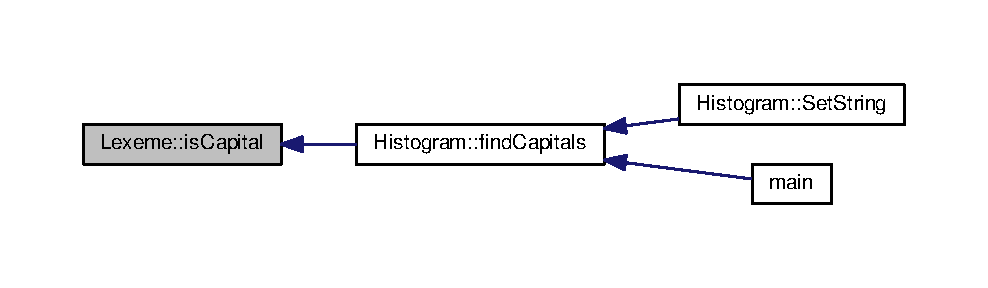
\includegraphics[width=350pt]{class_lexeme_afa5bf60e2cd601b4755cc137c56f7aed_icgraph}
\end{center}
\end{figure}
\mbox{\Hypertarget{class_lexeme_a67fb5732247889cb97612dd327c7a194}\label{class_lexeme_a67fb5732247889cb97612dd327c7a194}} 
\index{Lexeme@{Lexeme}!is\+Punctuation@{is\+Punctuation}}
\index{is\+Punctuation@{is\+Punctuation}!Lexeme@{Lexeme}}
\subsubsection{\texorpdfstring{is\+Punctuation()}{isPunctuation()}}
{\footnotesize\ttfamily int Lexeme\+::is\+Punctuation (\begin{DoxyParamCaption}{ }\end{DoxyParamCaption}) const\hspace{0.3cm}{\ttfamily [inline]}}

Here is the caller graph for this function\+:
\nopagebreak
\begin{figure}[H]
\begin{center}
\leavevmode
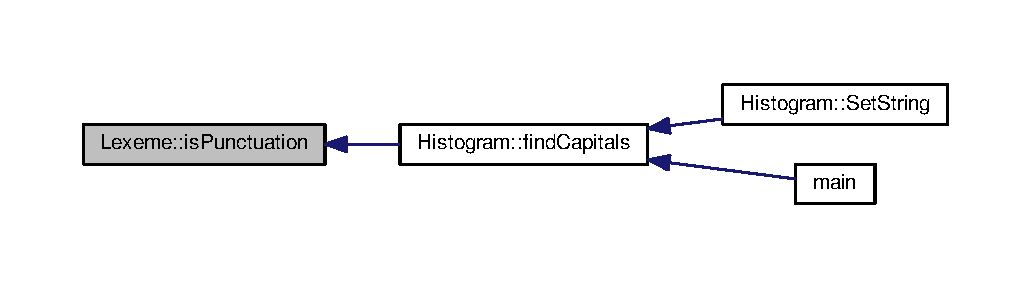
\includegraphics[width=350pt]{class_lexeme_a67fb5732247889cb97612dd327c7a194_icgraph}
\end{center}
\end{figure}
\mbox{\Hypertarget{class_lexeme_a8fd310c078c13d53dc601c299d0acb78}\label{class_lexeme_a8fd310c078c13d53dc601c299d0acb78}} 
\index{Lexeme@{Lexeme}!set\+Ambiguous@{set\+Ambiguous}}
\index{set\+Ambiguous@{set\+Ambiguous}!Lexeme@{Lexeme}}
\subsubsection{\texorpdfstring{set\+Ambiguous()}{setAmbiguous()}}
{\footnotesize\ttfamily void Lexeme\+::set\+Ambiguous (\begin{DoxyParamCaption}\item[{bool}]{amb }\end{DoxyParamCaption})\hspace{0.3cm}{\ttfamily [inline]}}

Here is the caller graph for this function\+:
\nopagebreak
\begin{figure}[H]
\begin{center}
\leavevmode
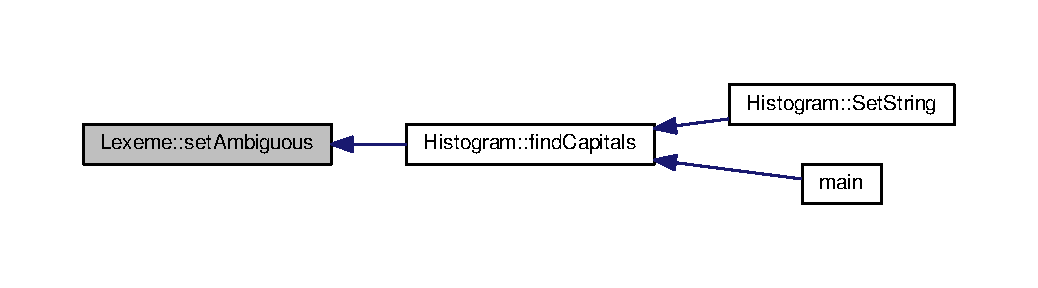
\includegraphics[width=350pt]{class_lexeme_a8fd310c078c13d53dc601c299d0acb78_icgraph}
\end{center}
\end{figure}
\mbox{\Hypertarget{class_lexeme_aa54d86594141f95df8a0364aebc931f2}\label{class_lexeme_aa54d86594141f95df8a0364aebc931f2}} 
\index{Lexeme@{Lexeme}!set\+Capital@{set\+Capital}}
\index{set\+Capital@{set\+Capital}!Lexeme@{Lexeme}}
\subsubsection{\texorpdfstring{set\+Capital()}{setCapital()}}
{\footnotesize\ttfamily void Lexeme\+::set\+Capital (\begin{DoxyParamCaption}\item[{bool}]{cap }\end{DoxyParamCaption})\hspace{0.3cm}{\ttfamily [inline]}}

\mbox{\Hypertarget{class_lexeme_a4bf15e88113bc3cd10dff188fef37752}\label{class_lexeme_a4bf15e88113bc3cd10dff188fef37752}} 
\index{Lexeme@{Lexeme}!set\+Digit@{set\+Digit}}
\index{set\+Digit@{set\+Digit}!Lexeme@{Lexeme}}
\subsubsection{\texorpdfstring{set\+Digit()}{setDigit()}}
{\footnotesize\ttfamily void Lexeme\+::set\+Digit (\begin{DoxyParamCaption}\item[{bool}]{digi }\end{DoxyParamCaption})\hspace{0.3cm}{\ttfamily [inline]}}

\mbox{\Hypertarget{class_lexeme_a620288e33ed2b3957023b3d325febc13}\label{class_lexeme_a620288e33ed2b3957023b3d325febc13}} 
\index{Lexeme@{Lexeme}!set\+Punctuation@{set\+Punctuation}}
\index{set\+Punctuation@{set\+Punctuation}!Lexeme@{Lexeme}}
\subsubsection{\texorpdfstring{set\+Punctuation()}{setPunctuation()}}
{\footnotesize\ttfamily void Lexeme\+::set\+Punctuation (\begin{DoxyParamCaption}\item[{int}]{punct }\end{DoxyParamCaption})\hspace{0.3cm}{\ttfamily [inline]}}

\mbox{\Hypertarget{class_lexeme_a90a1a2080fb503b0a206a075fd4d038a}\label{class_lexeme_a90a1a2080fb503b0a206a075fd4d038a}} 
\index{Lexeme@{Lexeme}!set\+String@{set\+String}}
\index{set\+String@{set\+String}!Lexeme@{Lexeme}}
\subsubsection{\texorpdfstring{set\+String()}{setString()}}
{\footnotesize\ttfamily void Lexeme\+::set\+String (\begin{DoxyParamCaption}\item[{string}]{s }\end{DoxyParamCaption})\hspace{0.3cm}{\ttfamily [inline]}}

Here is the caller graph for this function\+:
\nopagebreak
\begin{figure}[H]
\begin{center}
\leavevmode
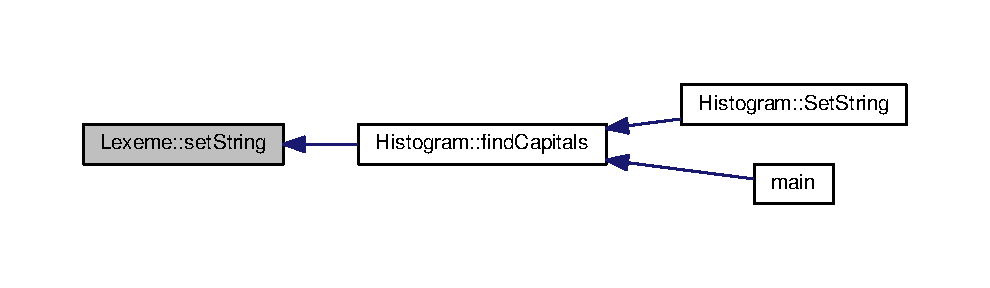
\includegraphics[width=350pt]{class_lexeme_a90a1a2080fb503b0a206a075fd4d038a_icgraph}
\end{center}
\end{figure}
\mbox{\Hypertarget{class_lexeme_a09873449eb90bc9be0f4df1edcf97b26}\label{class_lexeme_a09873449eb90bc9be0f4df1edcf97b26}} 
\index{Lexeme@{Lexeme}!set\+Upper@{set\+Upper}}
\index{set\+Upper@{set\+Upper}!Lexeme@{Lexeme}}
\subsubsection{\texorpdfstring{set\+Upper()}{setUpper()}}
{\footnotesize\ttfamily void Lexeme\+::set\+Upper (\begin{DoxyParamCaption}\item[{bool}]{up }\end{DoxyParamCaption})\hspace{0.3cm}{\ttfamily [inline]}}



The documentation for this class was generated from the following file\+:\begin{DoxyCompactItemize}
\item 
\hyperlink{_lexeme_8h}{Lexeme.\+h}\end{DoxyCompactItemize}

\hypertarget{class_porter}{}\section{Porter Class Reference}
\label{class_porter}\index{Porter@{Porter}}


An implementation of the \hyperlink{class_porter}{Porter} Algorithm \#2.  




{\ttfamily \#include $<$Porter.\+h$>$}

\subsection*{Public Member Functions}
\begin{DoxyCompactItemize}
\item 
\hyperlink{class_porter_a04be3733ab5109a1cf6131de05cc5961}{Porter} ()
\begin{DoxyCompactList}\small\item\em Constructor. \end{DoxyCompactList}\item 
string \hyperlink{class_porter_a9e33d06b477f04db7c8cee07e85e8bcb}{get\+Region} (const string \&str) const
\item 
string \hyperlink{class_porter_a1420c413bb564a22e4fc0c6627e1870b}{get\+Region2} (const string \&str) const
\item 
string \hyperlink{class_porter_a2000ce7eeabb3a7d9593fa9790a4fdc4}{get\+Preceder} (const string \&str, const unsigned long long len) const
\item 
bool \hyperlink{class_porter_a7c8a4b3b6103ce655e8ffc8a3eba1897}{is\+Double} (const string \&str) const
\item 
bool \hyperlink{class_porter_a35b1cc5606d4e78d1f69ac4037fdde87}{is\+Short} (const string \&str) const
\item 
bool \hyperlink{class_porter_a36e6678f68a4cc29371cc0111a8c8860}{is\+Short\+Syllable} (const string \&str) const
\item 
bool \hyperlink{class_porter_ac53ad85d5d3178b72178a4d89137b55e}{is\+Validli} (const string \&str) const
\item 
bool \hyperlink{class_porter_ab16d2762c47b86b9a161be3d2c44203e}{is\+Vowel} (const string \&str, unsigned long long loc) const
\item 
bool \hyperlink{class_porter_a9da79dd6524131e703619d3e301e896a}{is\+Valid} (const string \&str) const
\item 
void \hyperlink{class_porter_aba12641d0e612b264097a35e4f2ffb45}{replace} (string \&str, const string replacement, const int length) const
\item 
void \hyperlink{class_porter_af7f1d6892ca1ed4e22986c48be2365d6}{Go\+Go\+Porter\+Numero\+Dos} (string \&str, unsigned long long size) const
\item 
void \hyperlink{class_porter_ad8b63c9741655393ff9c849d269c953a}{Stem\+Uno} (string \&str, const unsigned long long size) const
\item 
void \hyperlink{class_porter_a33838d3b5ab4963106a5c47c4a0c74e6}{Stem\+Dos} (string \&str, const unsigned long long size) const
\item 
void \hyperlink{class_porter_a4aadb1440bc5f143aba28641cab26ff6}{Stem\+Tres} (string \&str, const unsigned long long size) const
\item 
void \hyperlink{class_porter_ac5e4f3909a27316c6997c92a0019eaaf}{Stem\+Tres\+Alpha} (string \&str, const string \&preceder, const unsigned long long length) const
\item 
void \hyperlink{class_porter_aa1e1b416311f37b827bc093bb03ca500}{Stem\+Cuatro} (string \&str, const unsigned long long size) const
\item 
void \hyperlink{class_porter_a916f45b55a1bbdaff7ce1db3d9a42813}{Stem\+Cinco} (string \&str, const unsigned long long size) const
\item 
void \hyperlink{class_porter_a485f69d6797fce65144e0596f3190c2d}{Stem\+Seis} (string \&str, const unsigned long long size) const
\item 
void \hyperlink{class_porter_a1015f959403c55d740fff435f0cae439}{Stem\+Siete} (string \&str, const unsigned long long size) const
\item 
void \hyperlink{class_porter_a61853073641e47863fc6a85c786d8737}{Stem\+Ocho} (string \&str, const unsigned long long size) const
\item 
void \hyperlink{class_porter_afbe6ae10a924a4419e62a20babe3be7d}{Eval} (\hyperlink{class_histogram}{Histogram} \&Hist, unordered\+\_\+map$<$ string, string $>$ \&map) const
\end{DoxyCompactItemize}


\subsection{Detailed Description}
An implementation of the \hyperlink{class_porter}{Porter} Algorithm \#2. 

A class for parsing grammatical suffixes given specific conditions and replacements 

\subsection{Constructor \& Destructor Documentation}
\mbox{\Hypertarget{class_porter_a04be3733ab5109a1cf6131de05cc5961}\label{class_porter_a04be3733ab5109a1cf6131de05cc5961}} 
\index{Porter@{Porter}!Porter@{Porter}}
\index{Porter@{Porter}!Porter@{Porter}}
\subsubsection{\texorpdfstring{Porter()}{Porter()}}
{\footnotesize\ttfamily Porter\+::\+Porter (\begin{DoxyParamCaption}{ }\end{DoxyParamCaption})\hspace{0.3cm}{\ttfamily [inline]}}



Constructor. 

Here is the call graph for this function\+:
\nopagebreak
\begin{figure}[H]
\begin{center}
\leavevmode
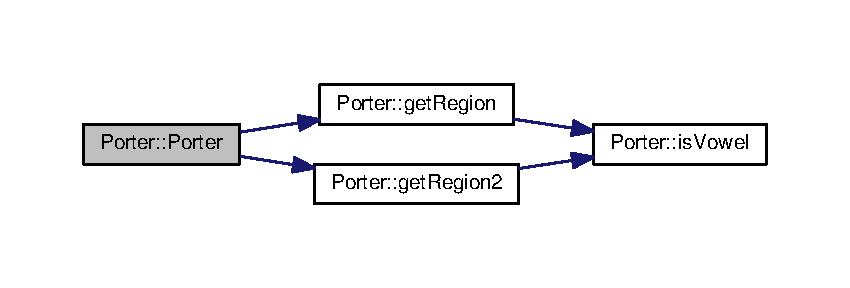
\includegraphics[width=350pt]{class_porter_a04be3733ab5109a1cf6131de05cc5961_cgraph}
\end{center}
\end{figure}


\subsection{Member Function Documentation}
\mbox{\Hypertarget{class_porter_afbe6ae10a924a4419e62a20babe3be7d}\label{class_porter_afbe6ae10a924a4419e62a20babe3be7d}} 
\index{Porter@{Porter}!Eval@{Eval}}
\index{Eval@{Eval}!Porter@{Porter}}
\subsubsection{\texorpdfstring{Eval()}{Eval()}}
{\footnotesize\ttfamily void Porter\+::\+Eval (\begin{DoxyParamCaption}\item[{\hyperlink{class_histogram}{Histogram} \&}]{Hist,  }\item[{unordered\+\_\+map$<$ string, string $>$ \&}]{map }\end{DoxyParamCaption}) const}

Evaluation operator. Takes a \hyperlink{class_histogram}{Histogram} and applies an 8-\/step algorithm to the strings within the .histogram in order to stem them before counting Here is the caller graph for this function\+:
\nopagebreak
\begin{figure}[H]
\begin{center}
\leavevmode
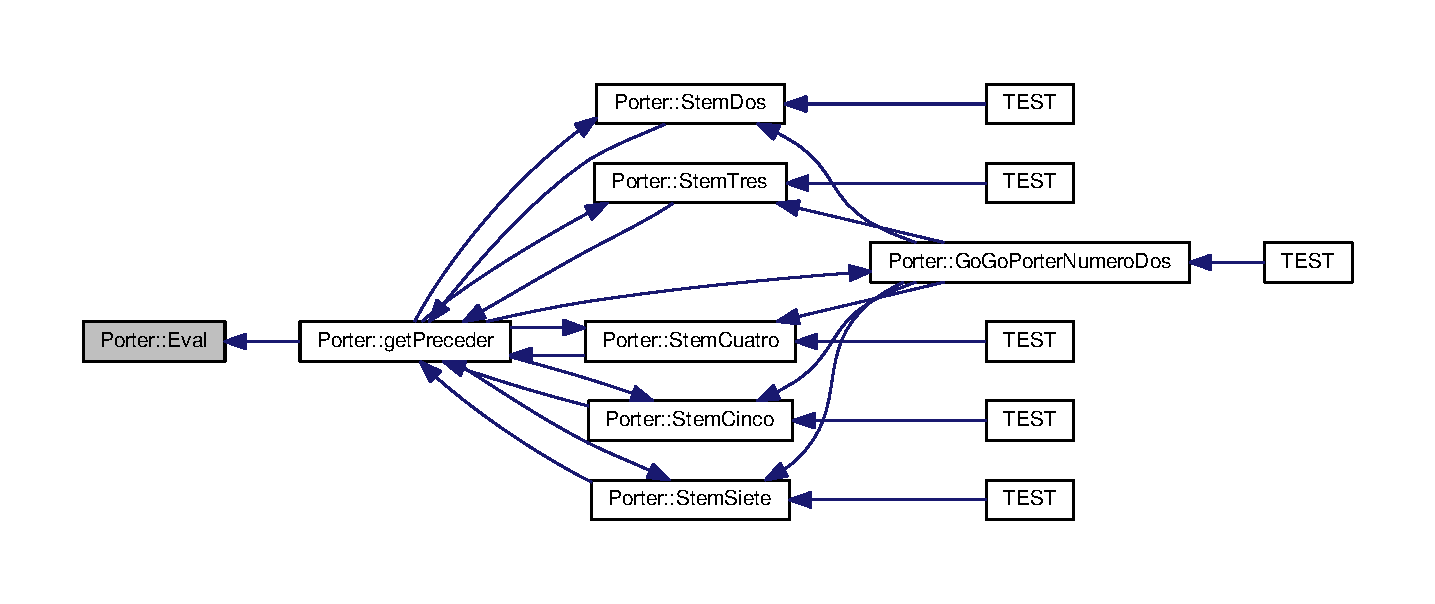
\includegraphics[width=350pt]{class_porter_afbe6ae10a924a4419e62a20babe3be7d_icgraph}
\end{center}
\end{figure}
\mbox{\Hypertarget{class_porter_a2000ce7eeabb3a7d9593fa9790a4fdc4}\label{class_porter_a2000ce7eeabb3a7d9593fa9790a4fdc4}} 
\index{Porter@{Porter}!get\+Preceder@{get\+Preceder}}
\index{get\+Preceder@{get\+Preceder}!Porter@{Porter}}
\subsubsection{\texorpdfstring{get\+Preceder()}{getPreceder()}}
{\footnotesize\ttfamily string Porter\+::get\+Preceder (\begin{DoxyParamCaption}\item[{const string \&}]{str,  }\item[{const unsigned long long}]{len }\end{DoxyParamCaption}) const\hspace{0.3cm}{\ttfamily [inline]}}

Here is the call graph for this function\+:
\nopagebreak
\begin{figure}[H]
\begin{center}
\leavevmode
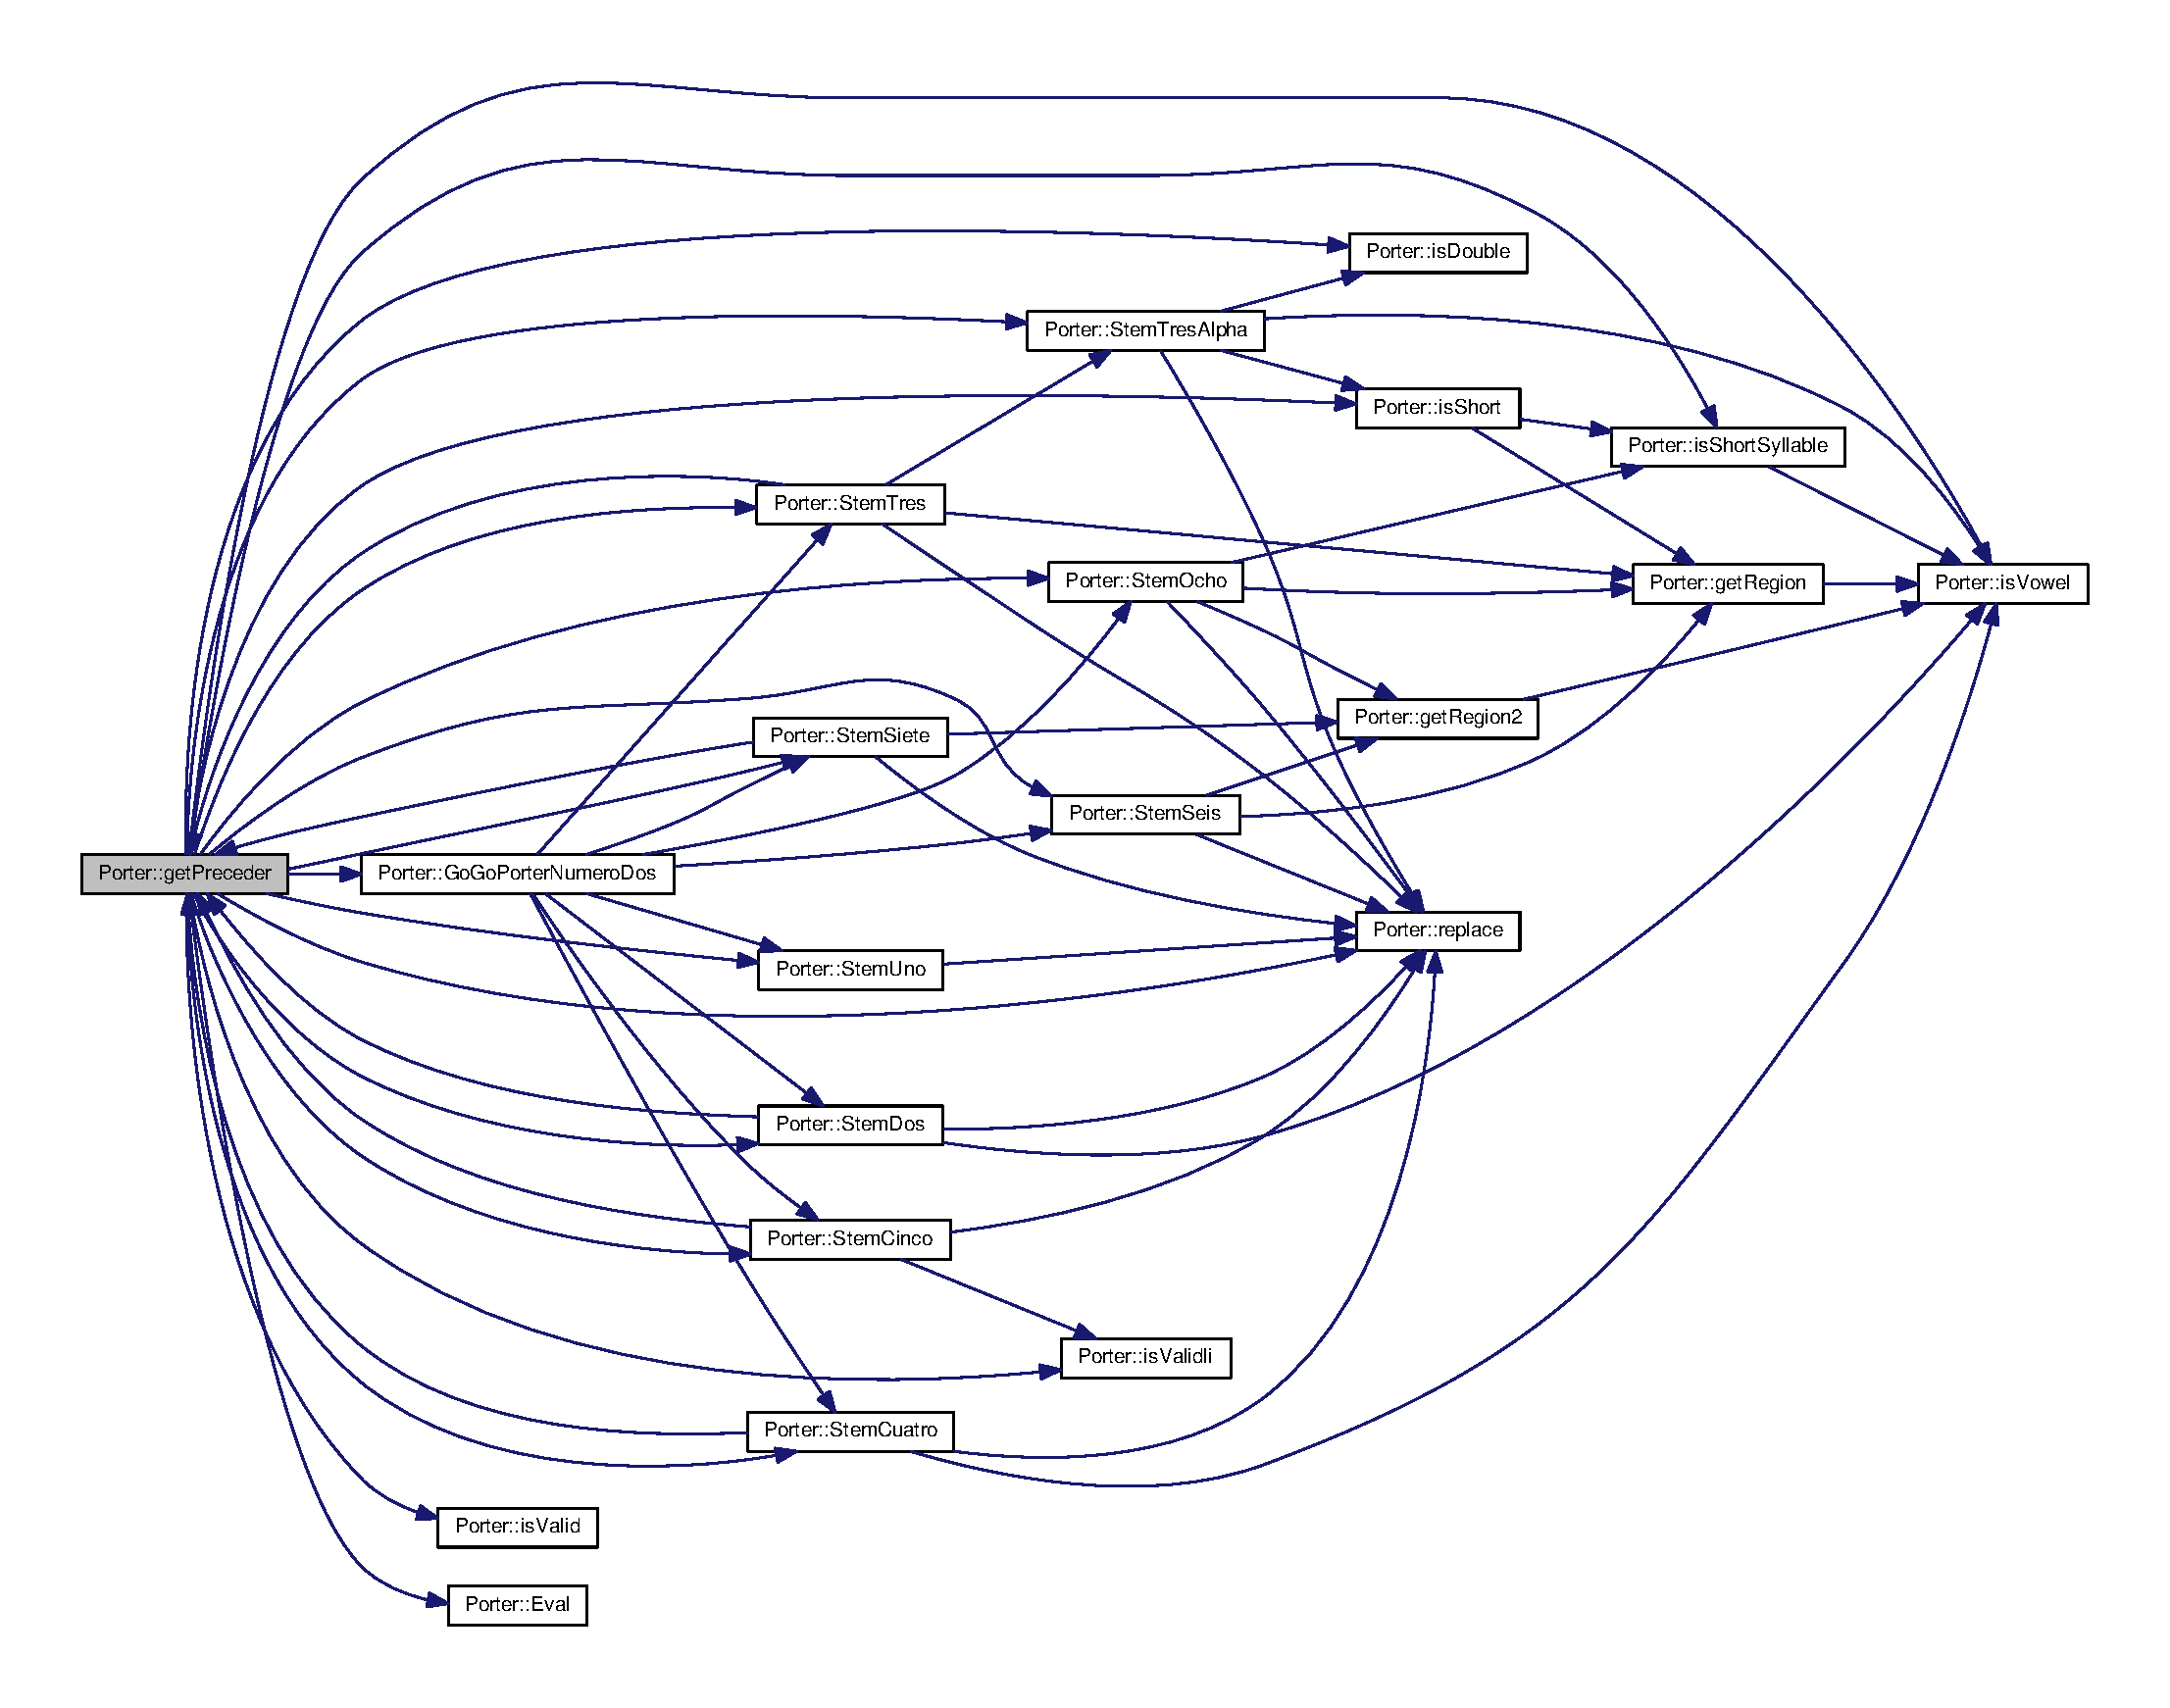
\includegraphics[width=350pt]{class_porter_a2000ce7eeabb3a7d9593fa9790a4fdc4_cgraph}
\end{center}
\end{figure}
Here is the caller graph for this function\+:
\nopagebreak
\begin{figure}[H]
\begin{center}
\leavevmode
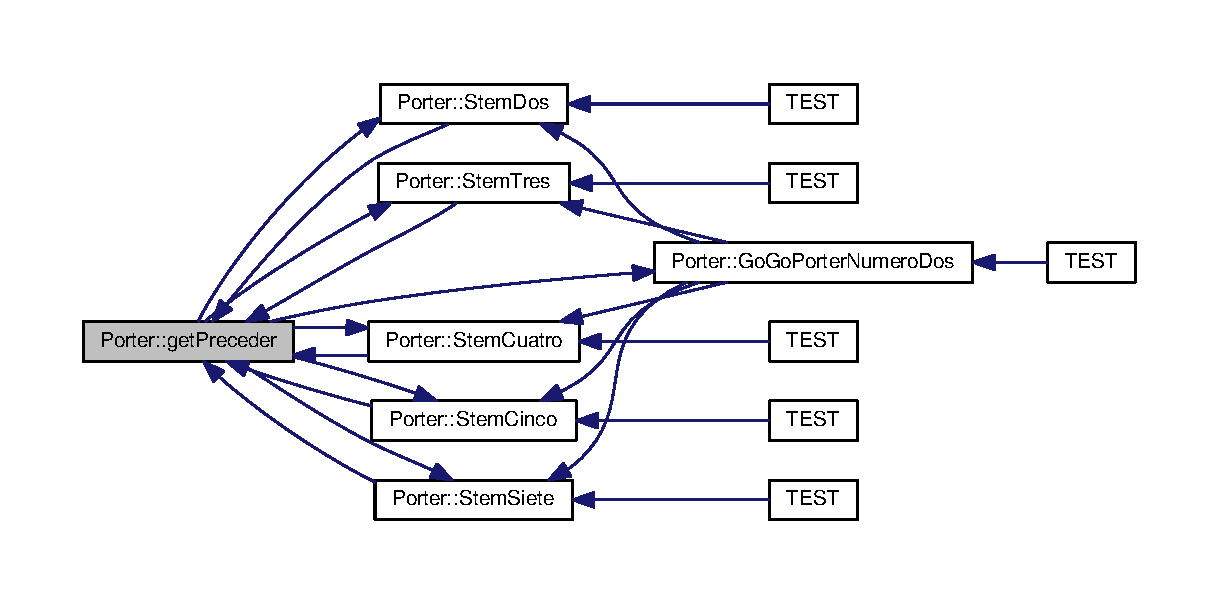
\includegraphics[width=350pt]{class_porter_a2000ce7eeabb3a7d9593fa9790a4fdc4_icgraph}
\end{center}
\end{figure}
\mbox{\Hypertarget{class_porter_a9e33d06b477f04db7c8cee07e85e8bcb}\label{class_porter_a9e33d06b477f04db7c8cee07e85e8bcb}} 
\index{Porter@{Porter}!get\+Region@{get\+Region}}
\index{get\+Region@{get\+Region}!Porter@{Porter}}
\subsubsection{\texorpdfstring{get\+Region()}{getRegion()}}
{\footnotesize\ttfamily string Porter\+::get\+Region (\begin{DoxyParamCaption}\item[{const string \&}]{str }\end{DoxyParamCaption}) const}

get\+Region(str) Takes a string and returns the defined \char`\"{}\+Region1\char`\"{} Here is the call graph for this function\+:
\nopagebreak
\begin{figure}[H]
\begin{center}
\leavevmode
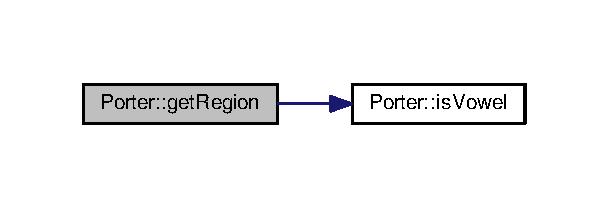
\includegraphics[width=292pt]{class_porter_a9e33d06b477f04db7c8cee07e85e8bcb_cgraph}
\end{center}
\end{figure}
Here is the caller graph for this function\+:
\nopagebreak
\begin{figure}[H]
\begin{center}
\leavevmode
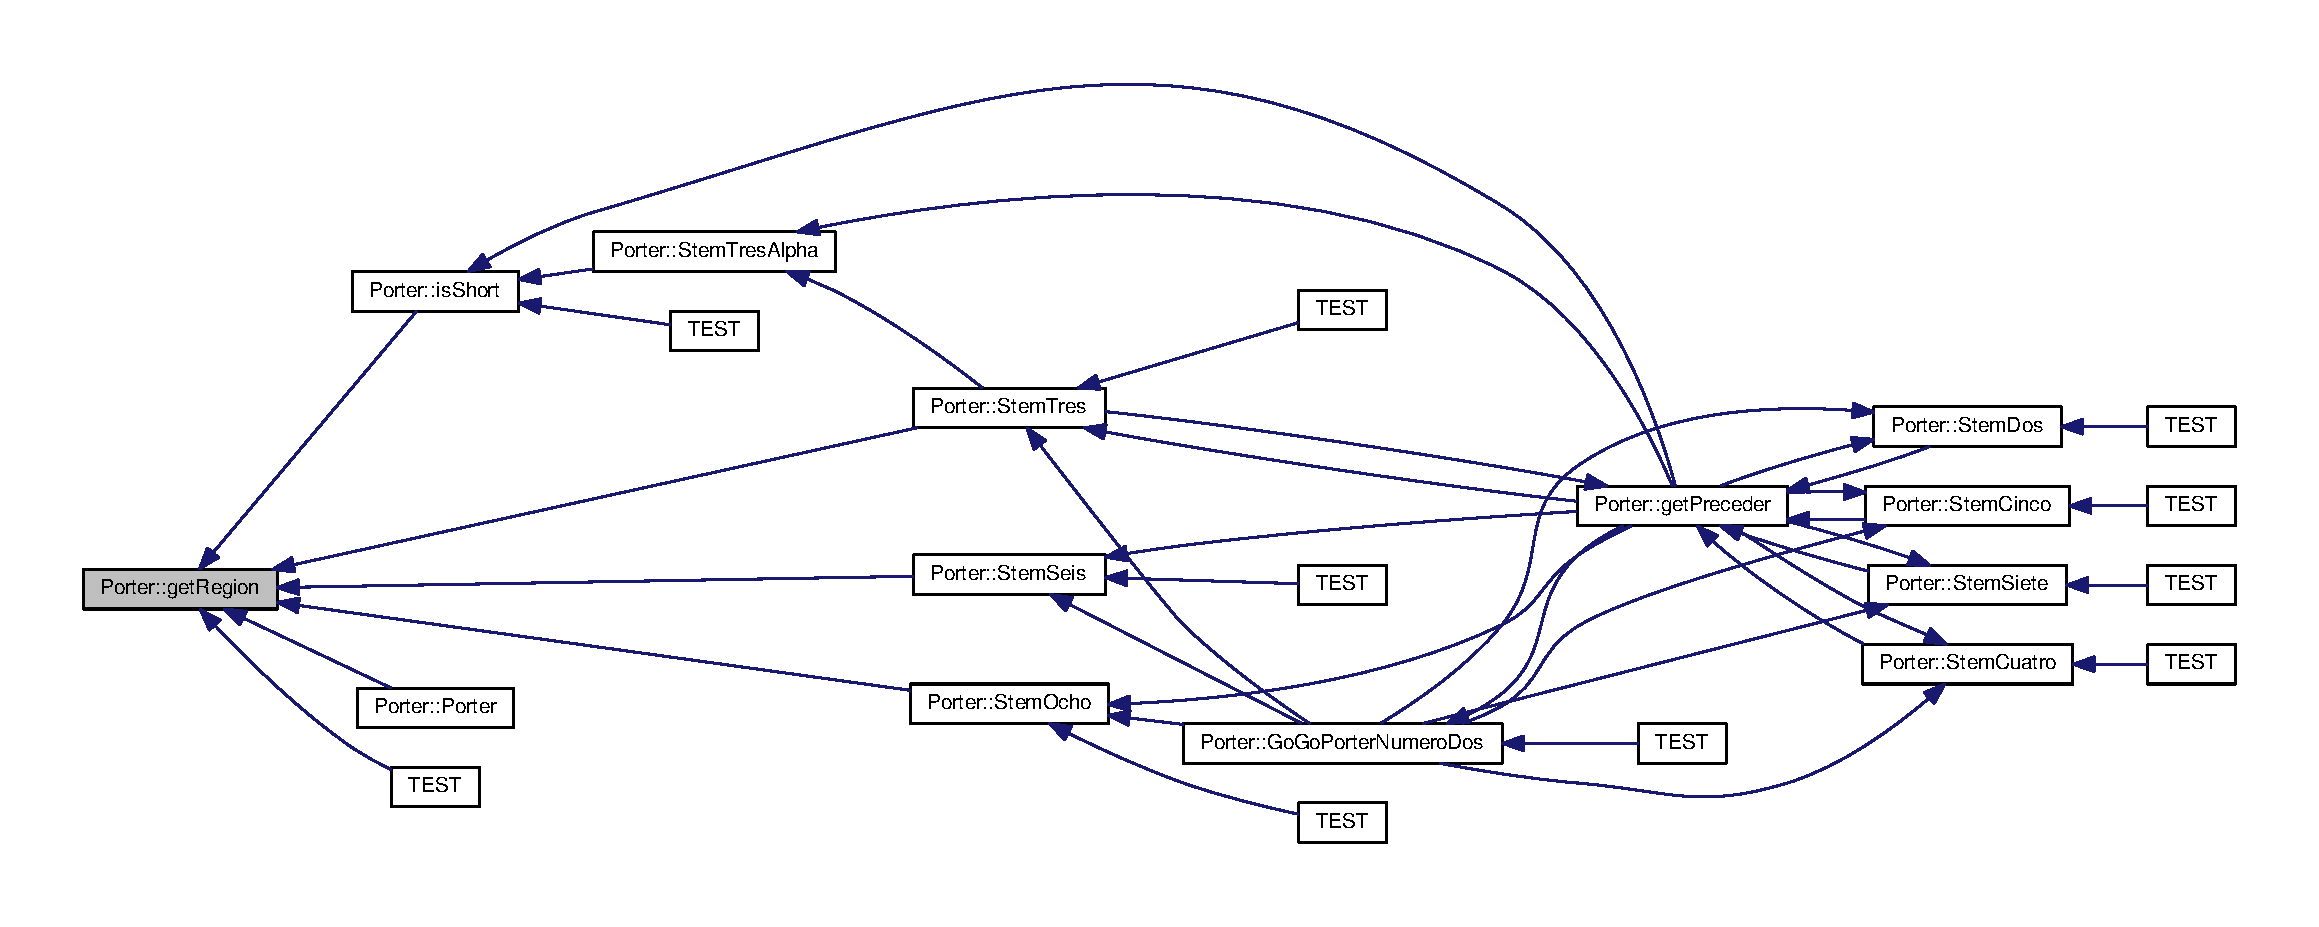
\includegraphics[width=350pt]{class_porter_a9e33d06b477f04db7c8cee07e85e8bcb_icgraph}
\end{center}
\end{figure}
\mbox{\Hypertarget{class_porter_a1420c413bb564a22e4fc0c6627e1870b}\label{class_porter_a1420c413bb564a22e4fc0c6627e1870b}} 
\index{Porter@{Porter}!get\+Region2@{get\+Region2}}
\index{get\+Region2@{get\+Region2}!Porter@{Porter}}
\subsubsection{\texorpdfstring{get\+Region2()}{getRegion2()}}
{\footnotesize\ttfamily string Porter\+::get\+Region2 (\begin{DoxyParamCaption}\item[{const string \&}]{str }\end{DoxyParamCaption}) const}

get\+Region2(str) Takes a string and returns the defined \char`\"{}\+Region2\char`\"{} R\+E\+L\+A\+T\+I\+VE TO T\+HE O\+R\+I\+G\+I\+N\+AL W\+O\+RD P\+ER IN C\+L\+A\+SS D\+I\+S\+C\+U\+S\+S\+I\+ON 10/10 Here is the call graph for this function\+:
\nopagebreak
\begin{figure}[H]
\begin{center}
\leavevmode
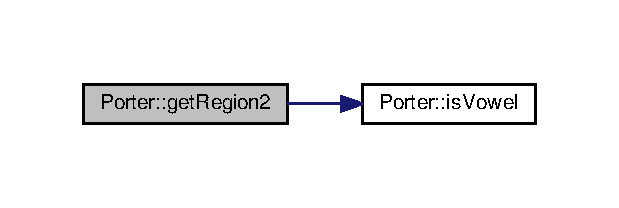
\includegraphics[width=297pt]{class_porter_a1420c413bb564a22e4fc0c6627e1870b_cgraph}
\end{center}
\end{figure}
Here is the caller graph for this function\+:
\nopagebreak
\begin{figure}[H]
\begin{center}
\leavevmode
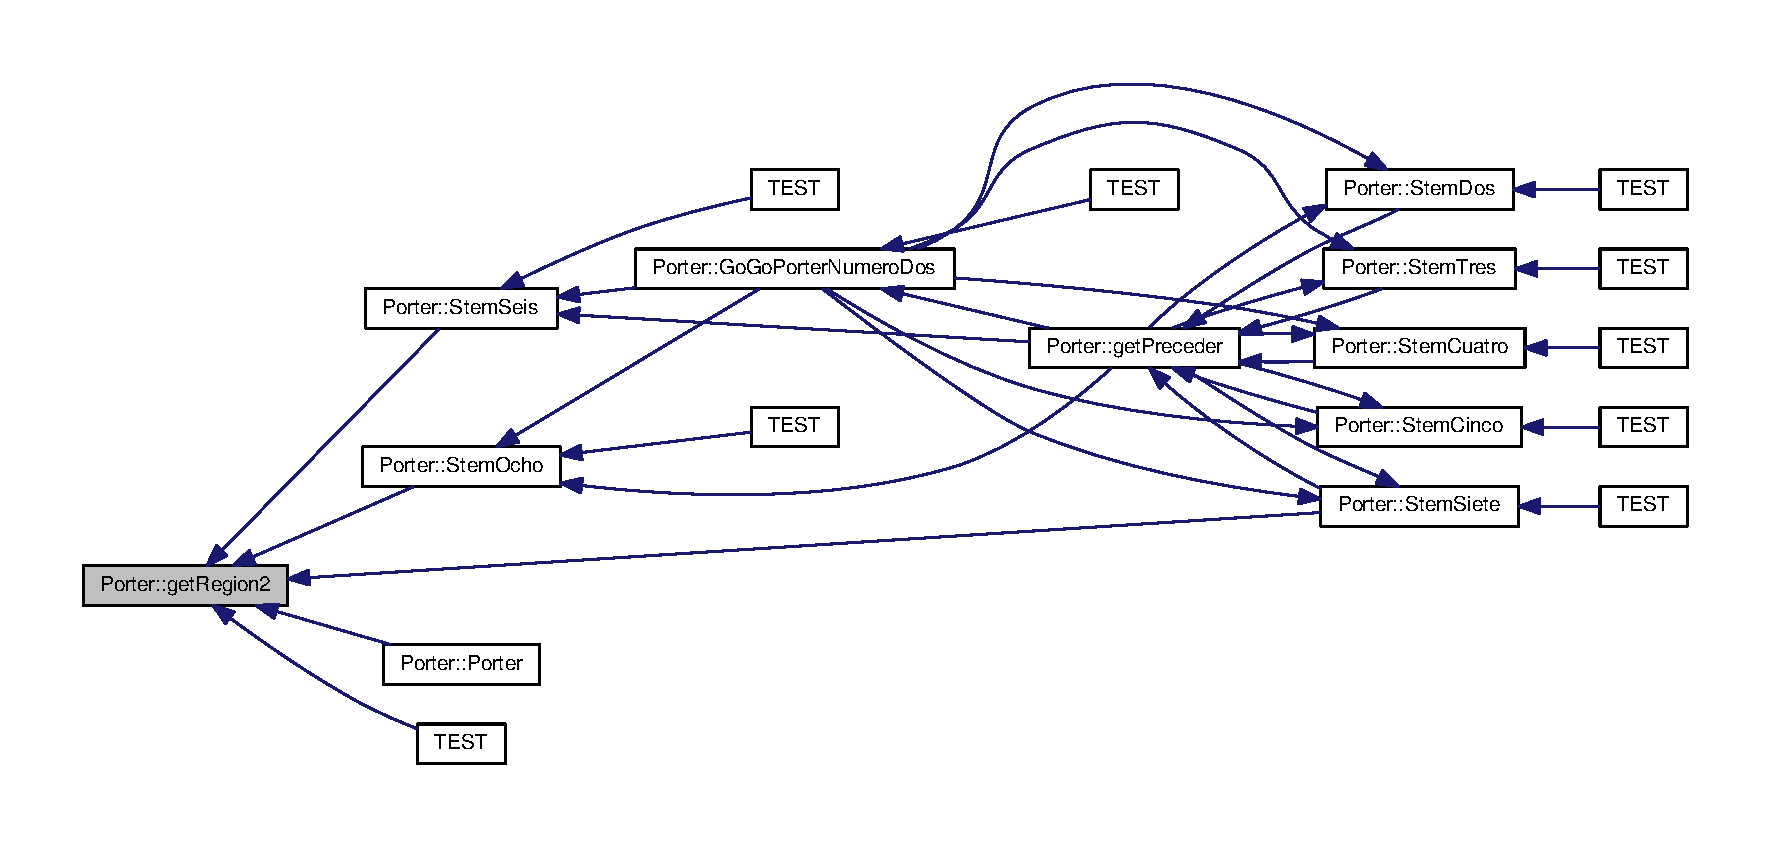
\includegraphics[width=350pt]{class_porter_a1420c413bb564a22e4fc0c6627e1870b_icgraph}
\end{center}
\end{figure}
\mbox{\Hypertarget{class_porter_af7f1d6892ca1ed4e22986c48be2365d6}\label{class_porter_af7f1d6892ca1ed4e22986c48be2365d6}} 
\index{Porter@{Porter}!Go\+Go\+Porter\+Numero\+Dos@{Go\+Go\+Porter\+Numero\+Dos}}
\index{Go\+Go\+Porter\+Numero\+Dos@{Go\+Go\+Porter\+Numero\+Dos}!Porter@{Porter}}
\subsubsection{\texorpdfstring{Go\+Go\+Porter\+Numero\+Dos()}{GoGoPorterNumeroDos()}}
{\footnotesize\ttfamily void Porter\+::\+Go\+Go\+Porter\+Numero\+Dos (\begin{DoxyParamCaption}\item[{string \&}]{str,  }\item[{unsigned long long}]{size }\end{DoxyParamCaption}) const}

Execute \hyperlink{class_porter}{Porter} Algorithm \#2 Takes a string and its size iterates through \hyperlink{class_porter}{Porter}\#2 to systematically stem away the suffix Here is the call graph for this function\+:
\nopagebreak
\begin{figure}[H]
\begin{center}
\leavevmode
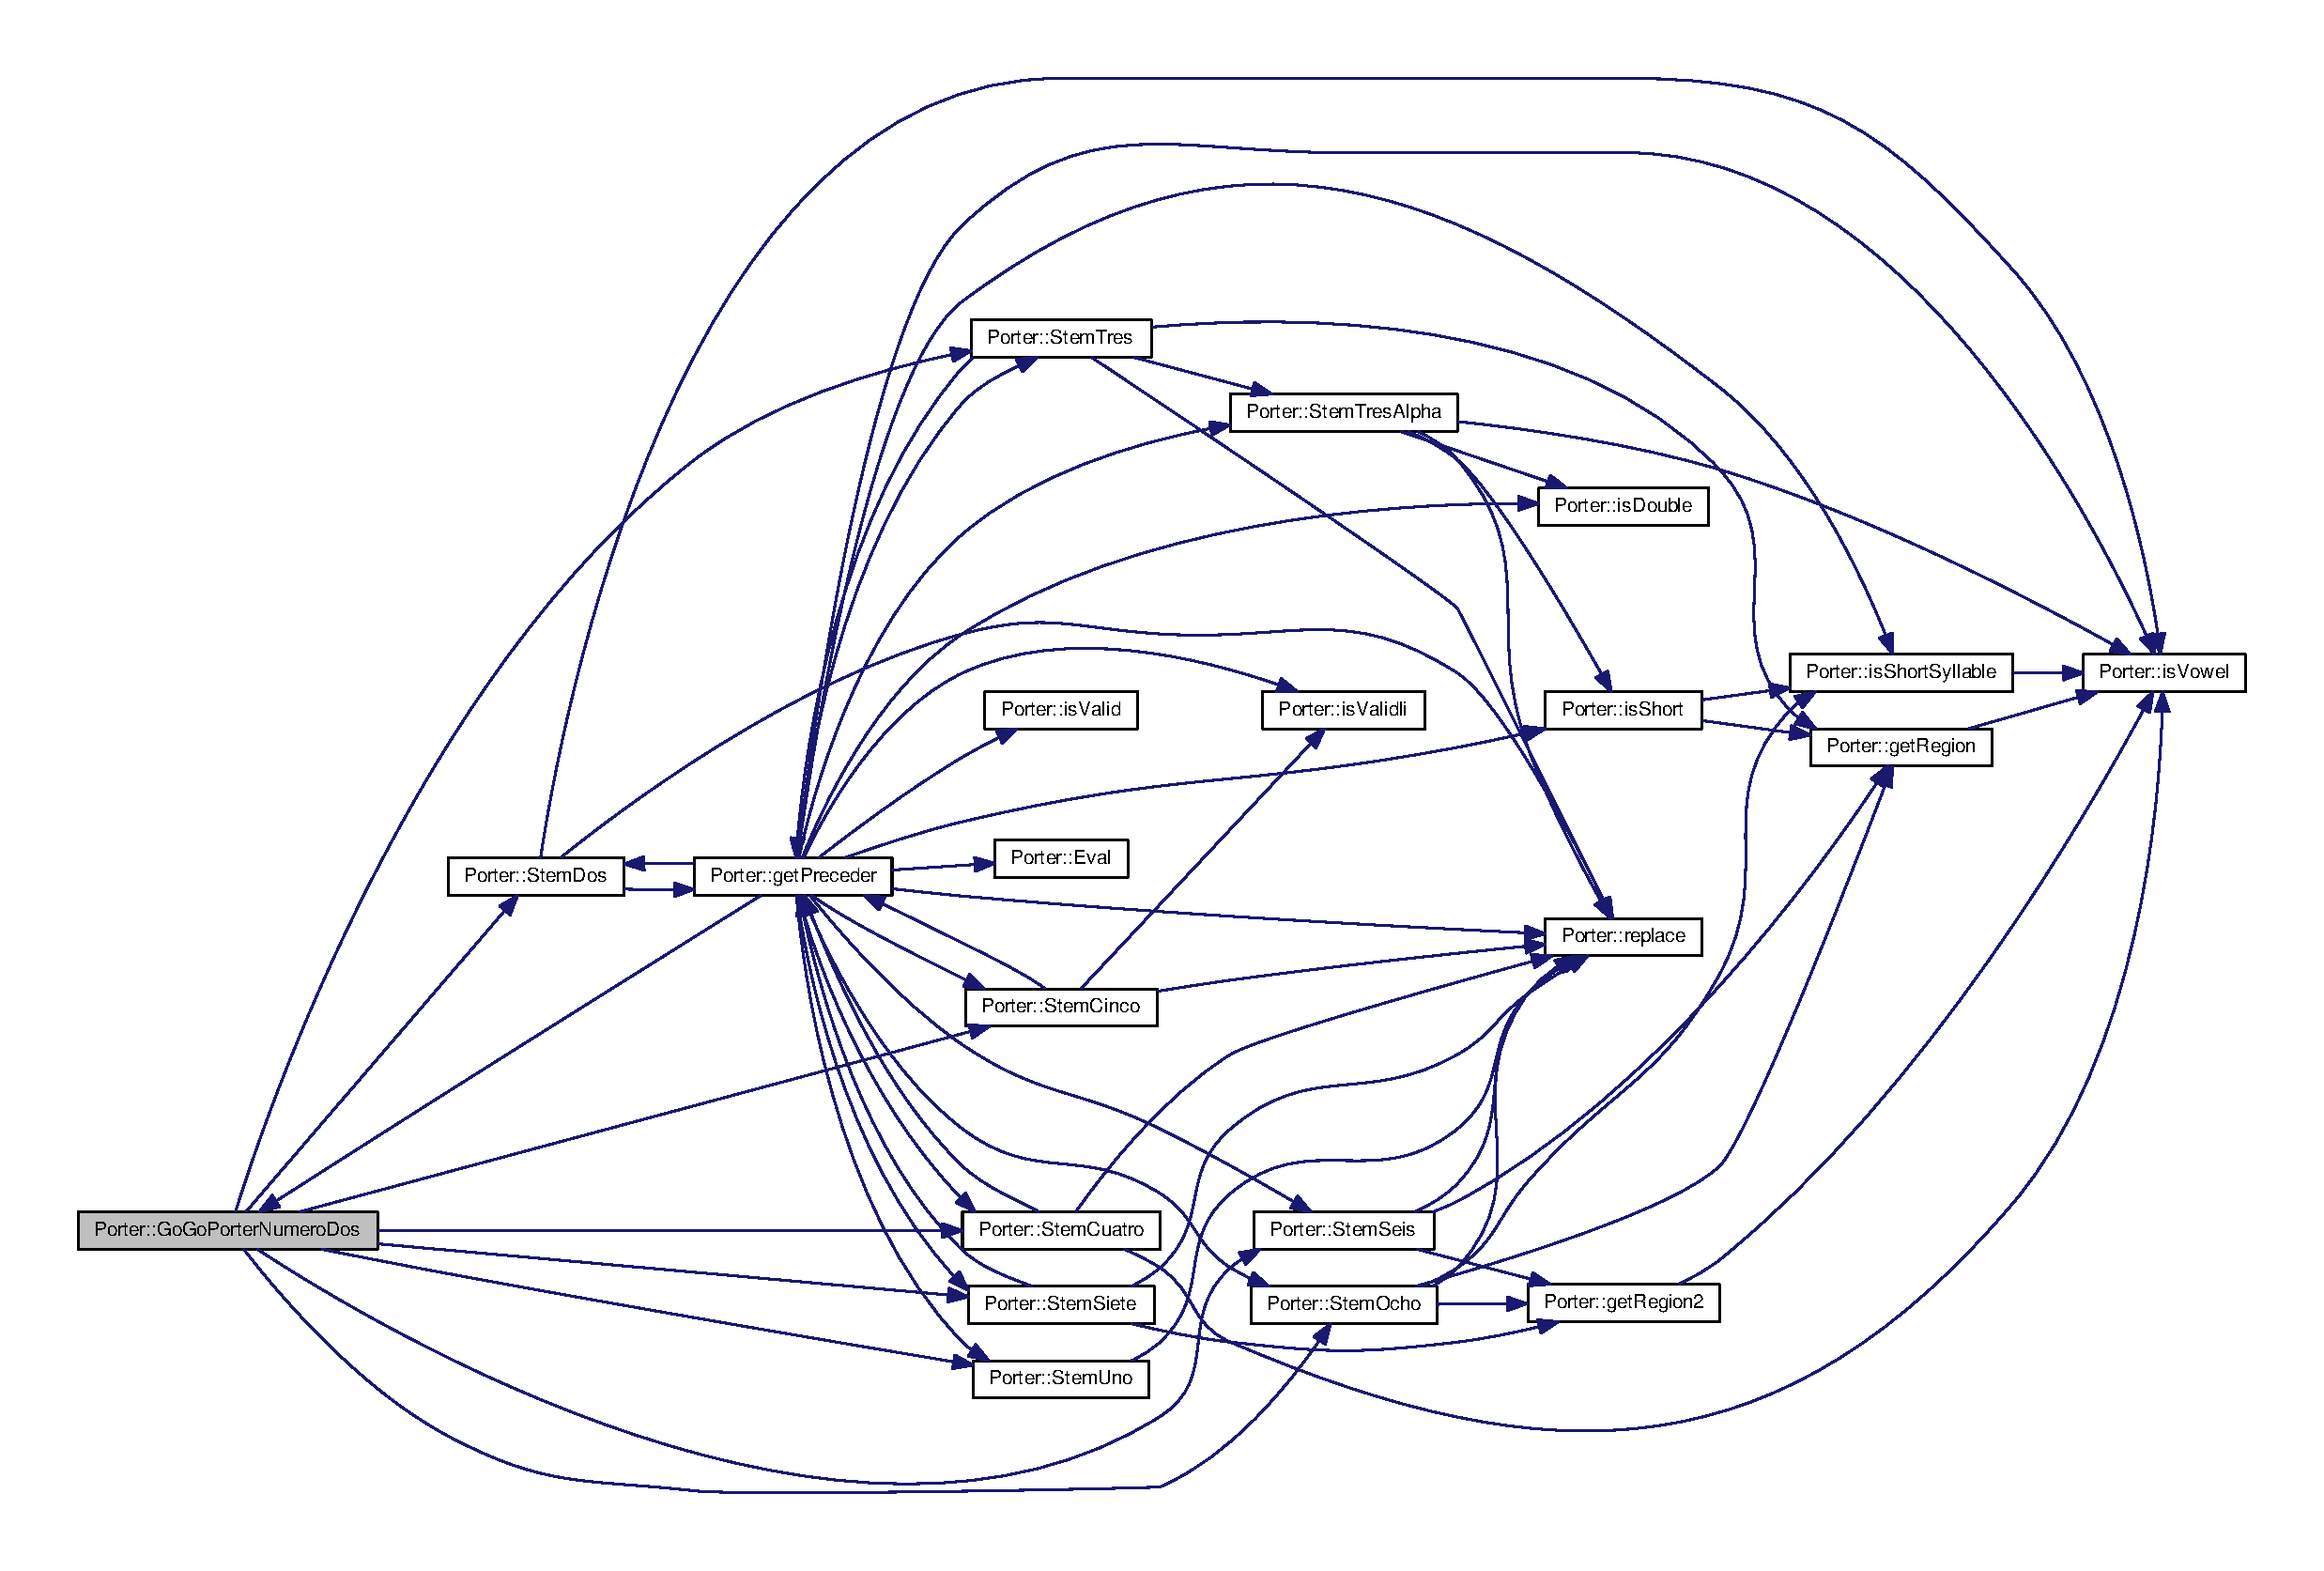
\includegraphics[width=350pt]{class_porter_af7f1d6892ca1ed4e22986c48be2365d6_cgraph}
\end{center}
\end{figure}
Here is the caller graph for this function\+:
\nopagebreak
\begin{figure}[H]
\begin{center}
\leavevmode
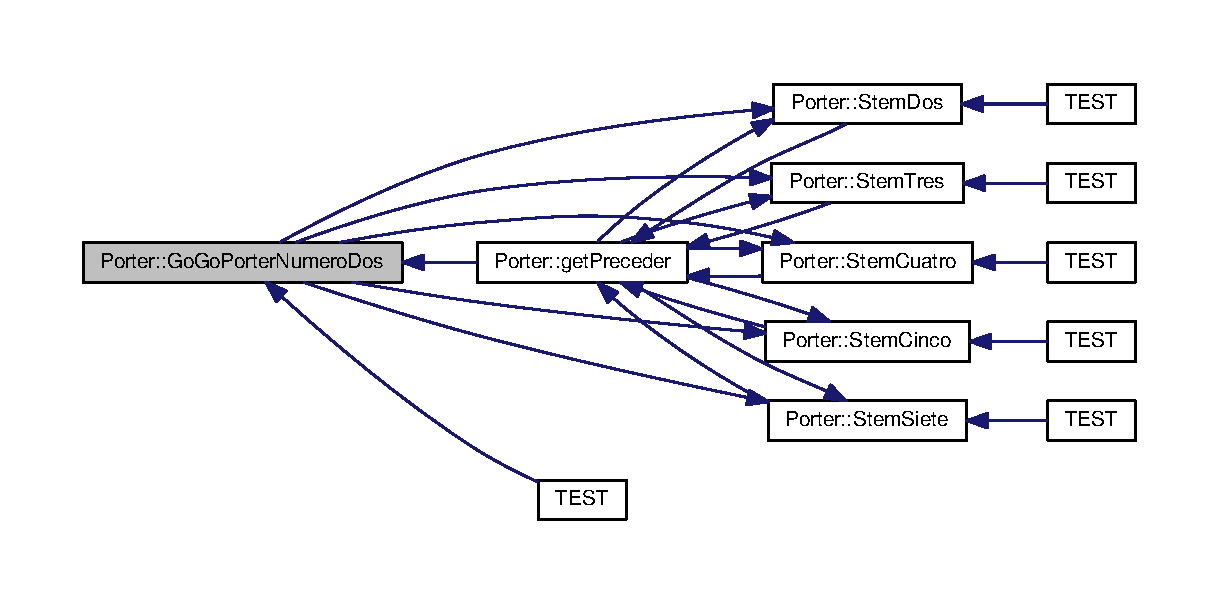
\includegraphics[width=350pt]{class_porter_af7f1d6892ca1ed4e22986c48be2365d6_icgraph}
\end{center}
\end{figure}
\mbox{\Hypertarget{class_porter_a7c8a4b3b6103ce655e8ffc8a3eba1897}\label{class_porter_a7c8a4b3b6103ce655e8ffc8a3eba1897}} 
\index{Porter@{Porter}!is\+Double@{is\+Double}}
\index{is\+Double@{is\+Double}!Porter@{Porter}}
\subsubsection{\texorpdfstring{is\+Double()}{isDouble()}}
{\footnotesize\ttfamily bool Porter\+::is\+Double (\begin{DoxyParamCaption}\item[{const string \&}]{str }\end{DoxyParamCaption}) const}

is\+Exception(str, size, map) Takes a string and a map of exceptions and checks to see if the string exists returns true if str is found in map is\+Double(str) Takes a string returns true if it is any of \{\textquotesingle{}bb\textquotesingle{}, \textquotesingle{}dd\textquotesingle{}, \textquotesingle{}ff\textquotesingle{}, \textquotesingle{}gg\textquotesingle{}, \textquotesingle{}mm\textquotesingle{}, \textquotesingle{}nn\textquotesingle{}, \textquotesingle{}pp\textquotesingle{}, \textquotesingle{}rr\textquotesingle{}, \textquotesingle{}tt\textquotesingle{}\} all other strings return false Here is the caller graph for this function\+:
\nopagebreak
\begin{figure}[H]
\begin{center}
\leavevmode
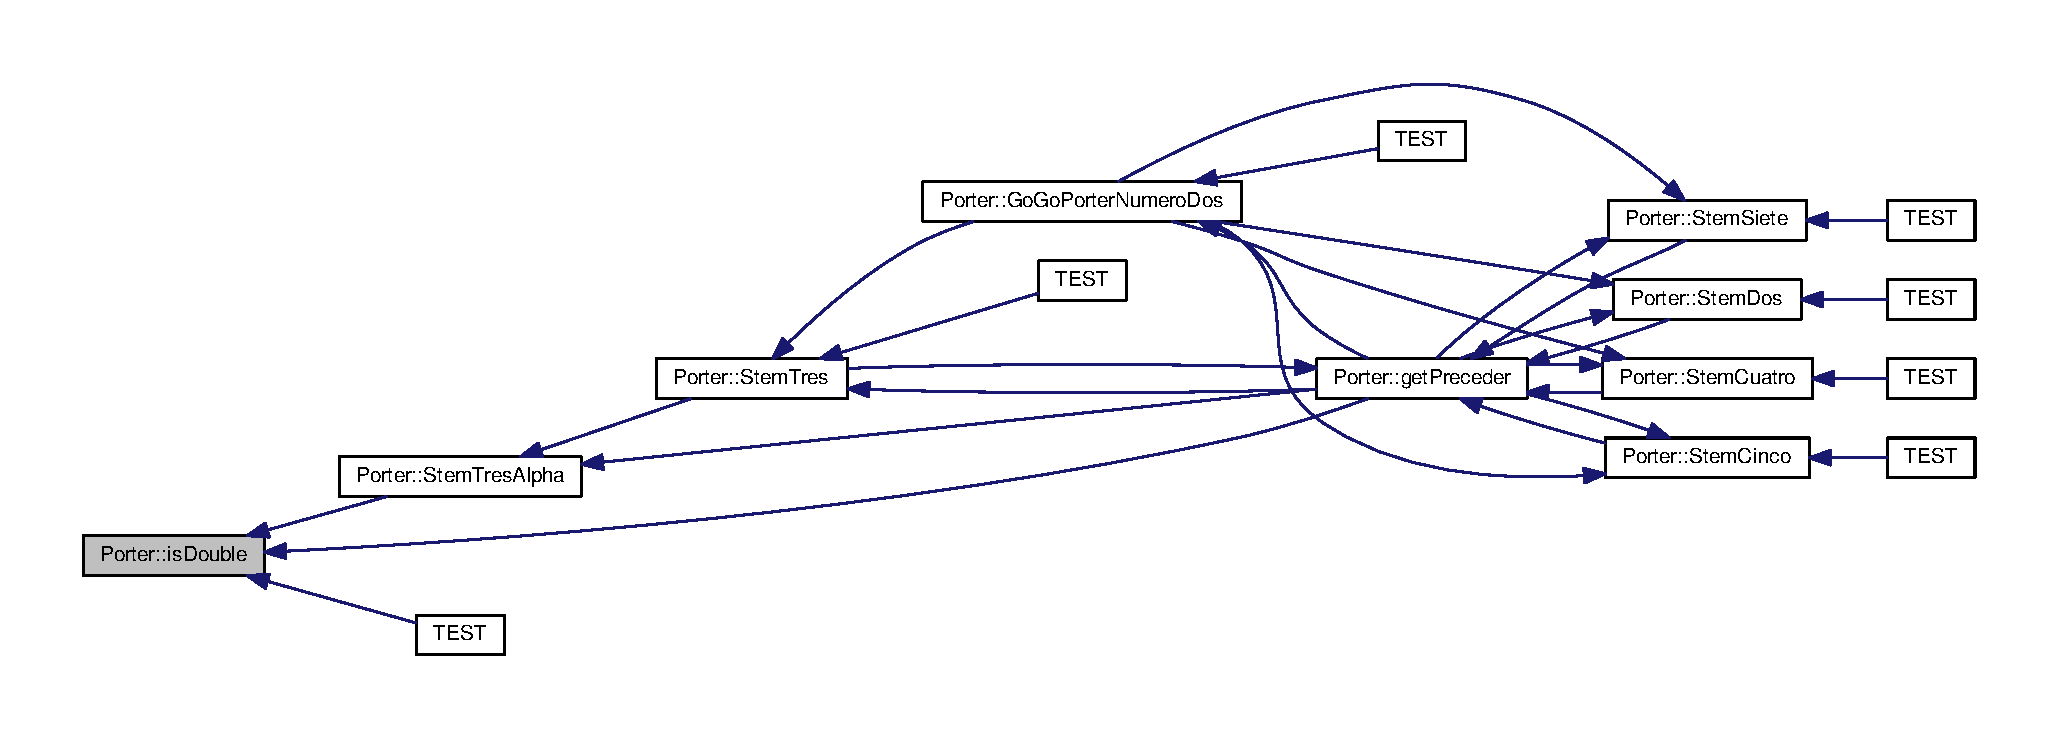
\includegraphics[width=350pt]{class_porter_a7c8a4b3b6103ce655e8ffc8a3eba1897_icgraph}
\end{center}
\end{figure}
\mbox{\Hypertarget{class_porter_a35b1cc5606d4e78d1f69ac4037fdde87}\label{class_porter_a35b1cc5606d4e78d1f69ac4037fdde87}} 
\index{Porter@{Porter}!is\+Short@{is\+Short}}
\index{is\+Short@{is\+Short}!Porter@{Porter}}
\subsubsection{\texorpdfstring{is\+Short()}{isShort()}}
{\footnotesize\ttfamily bool Porter\+::is\+Short (\begin{DoxyParamCaption}\item[{const string \&}]{str }\end{DoxyParamCaption}) const}

is\+Short(str) Takes a string returns true if it both 1) its Region1 is empty 2) it ends in a short-\/syllable Here is the call graph for this function\+:
\nopagebreak
\begin{figure}[H]
\begin{center}
\leavevmode
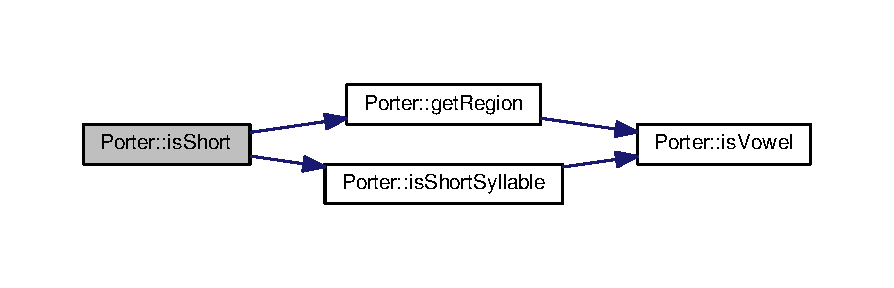
\includegraphics[width=350pt]{class_porter_a35b1cc5606d4e78d1f69ac4037fdde87_cgraph}
\end{center}
\end{figure}
Here is the caller graph for this function\+:
\nopagebreak
\begin{figure}[H]
\begin{center}
\leavevmode
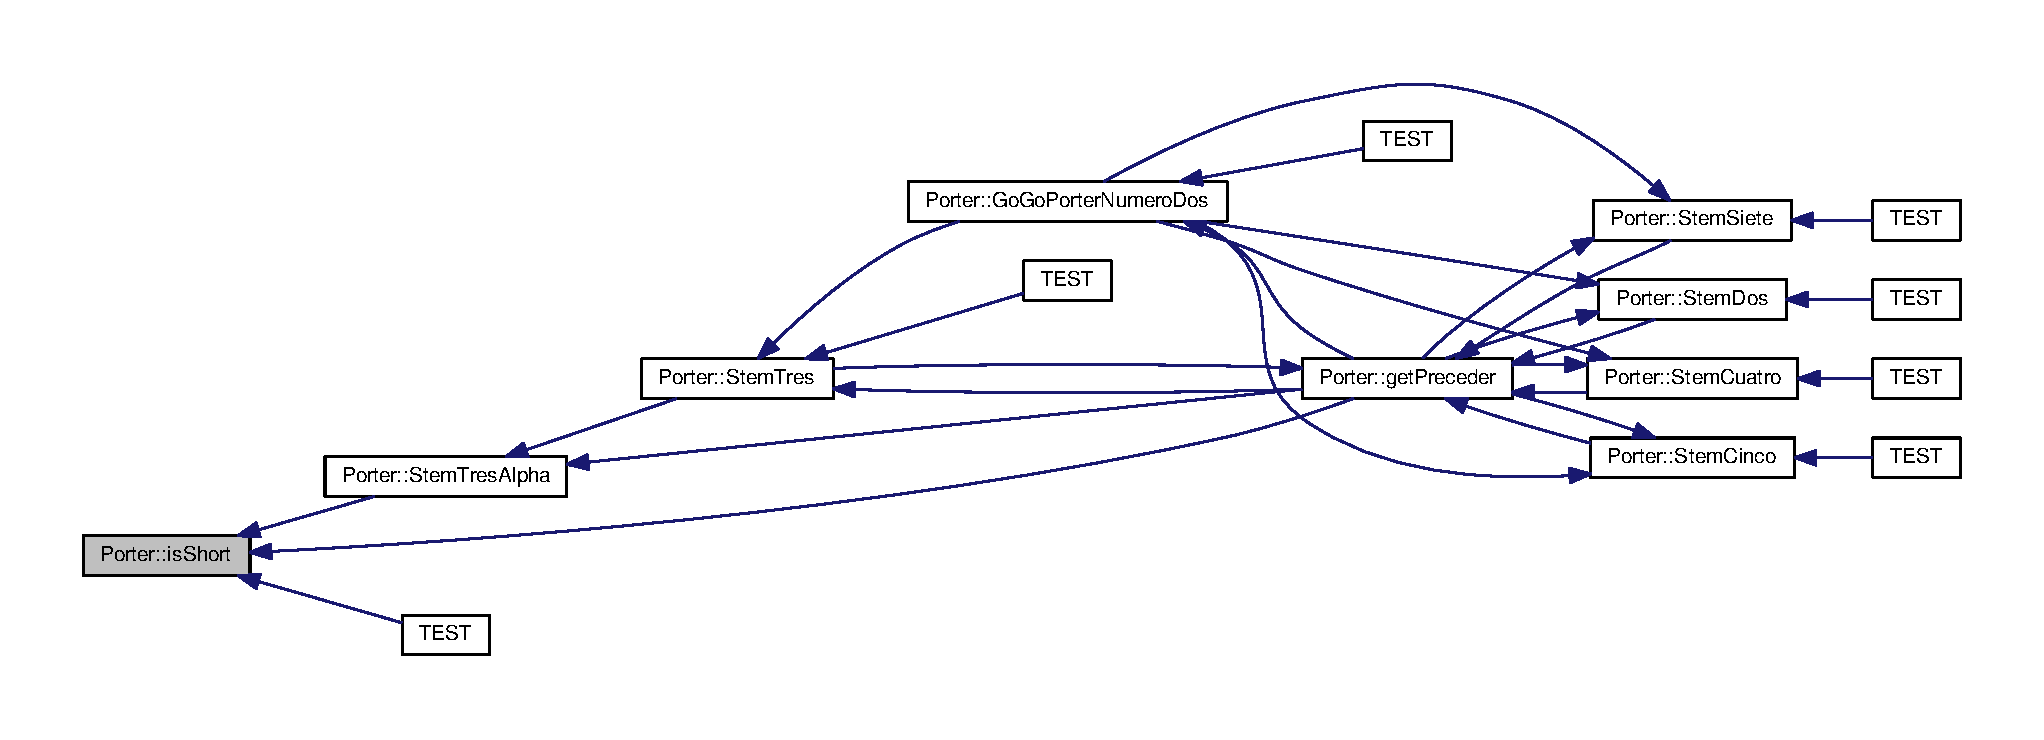
\includegraphics[width=350pt]{class_porter_a35b1cc5606d4e78d1f69ac4037fdde87_icgraph}
\end{center}
\end{figure}
\mbox{\Hypertarget{class_porter_a36e6678f68a4cc29371cc0111a8c8860}\label{class_porter_a36e6678f68a4cc29371cc0111a8c8860}} 
\index{Porter@{Porter}!is\+Short\+Syllable@{is\+Short\+Syllable}}
\index{is\+Short\+Syllable@{is\+Short\+Syllable}!Porter@{Porter}}
\subsubsection{\texorpdfstring{is\+Short\+Syllable()}{isShortSyllable()}}
{\footnotesize\ttfamily bool Porter\+::is\+Short\+Syllable (\begin{DoxyParamCaption}\item[{const string \&}]{str }\end{DoxyParamCaption}) const}

is\+Short\+Syllable(str) Takes a string returns true if either 1) it is only 2 chars long and is a vowel followed by a non-\/vowel 2) ends with a non-\/vowel followed by a vowel followed by a non-\/vowel that is not \{\textquotesingle{}w\textquotesingle{}, \textquotesingle{}x\textquotesingle{}, \textquotesingle{}y\textquotesingle{}\} Here is the call graph for this function\+:
\nopagebreak
\begin{figure}[H]
\begin{center}
\leavevmode
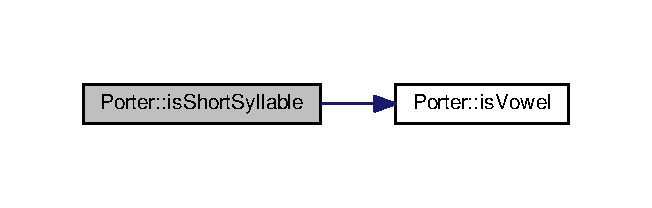
\includegraphics[width=313pt]{class_porter_a36e6678f68a4cc29371cc0111a8c8860_cgraph}
\end{center}
\end{figure}
Here is the caller graph for this function\+:
\nopagebreak
\begin{figure}[H]
\begin{center}
\leavevmode
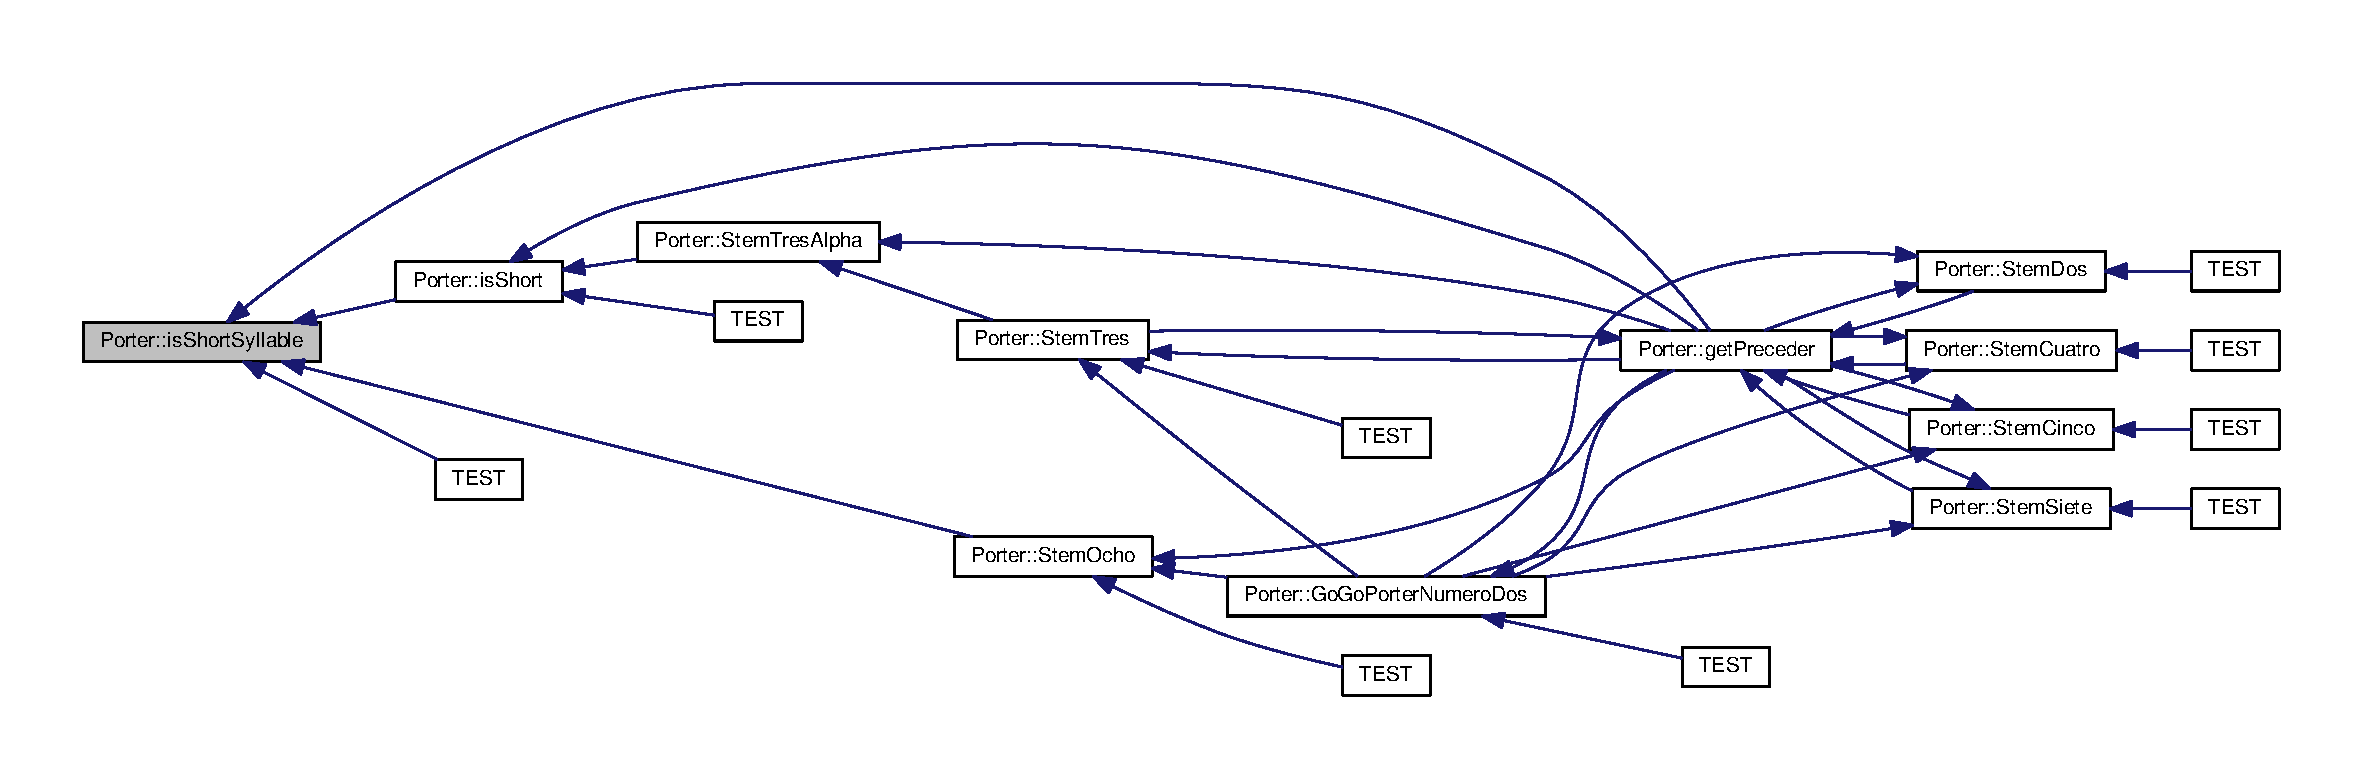
\includegraphics[width=350pt]{class_porter_a36e6678f68a4cc29371cc0111a8c8860_icgraph}
\end{center}
\end{figure}
\mbox{\Hypertarget{class_porter_a9da79dd6524131e703619d3e301e896a}\label{class_porter_a9da79dd6524131e703619d3e301e896a}} 
\index{Porter@{Porter}!is\+Valid@{is\+Valid}}
\index{is\+Valid@{is\+Valid}!Porter@{Porter}}
\subsubsection{\texorpdfstring{is\+Valid()}{isValid()}}
{\footnotesize\ttfamily bool Porter\+::is\+Valid (\begin{DoxyParamCaption}\item[{const string \&}]{str }\end{DoxyParamCaption}) const}

Here is the caller graph for this function\+:
\nopagebreak
\begin{figure}[H]
\begin{center}
\leavevmode
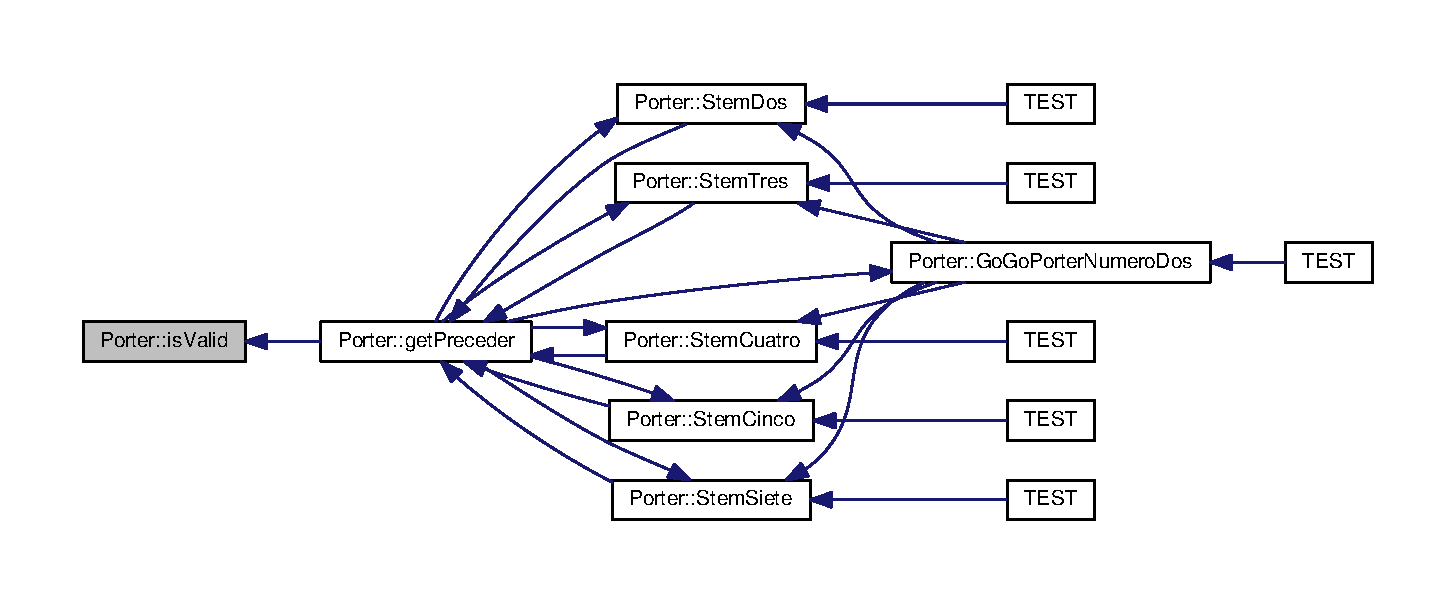
\includegraphics[width=350pt]{class_porter_a9da79dd6524131e703619d3e301e896a_icgraph}
\end{center}
\end{figure}
\mbox{\Hypertarget{class_porter_ac53ad85d5d3178b72178a4d89137b55e}\label{class_porter_ac53ad85d5d3178b72178a4d89137b55e}} 
\index{Porter@{Porter}!is\+Validli@{is\+Validli}}
\index{is\+Validli@{is\+Validli}!Porter@{Porter}}
\subsubsection{\texorpdfstring{is\+Validli()}{isValidli()}}
{\footnotesize\ttfamily bool Porter\+::is\+Validli (\begin{DoxyParamCaption}\item[{const string \&}]{str }\end{DoxyParamCaption}) const}

is\+Validli(str) Takes a string (preceder to an li-\/ending) returns true if it is any of \{\textquotesingle{}c\textquotesingle{}, \textquotesingle{}d\textquotesingle{}, \textquotesingle{}e\textquotesingle{}, \textquotesingle{}g\textquotesingle{}, \textquotesingle{}h\textquotesingle{}, \textquotesingle{}k\textquotesingle{}, \textquotesingle{}m\textquotesingle{}, \textquotesingle{}n\textquotesingle{}, \textquotesingle{}r\textquotesingle{}, \textquotesingle{}t\textquotesingle{}\} all other chars return false; Here is the caller graph for this function\+:
\nopagebreak
\begin{figure}[H]
\begin{center}
\leavevmode
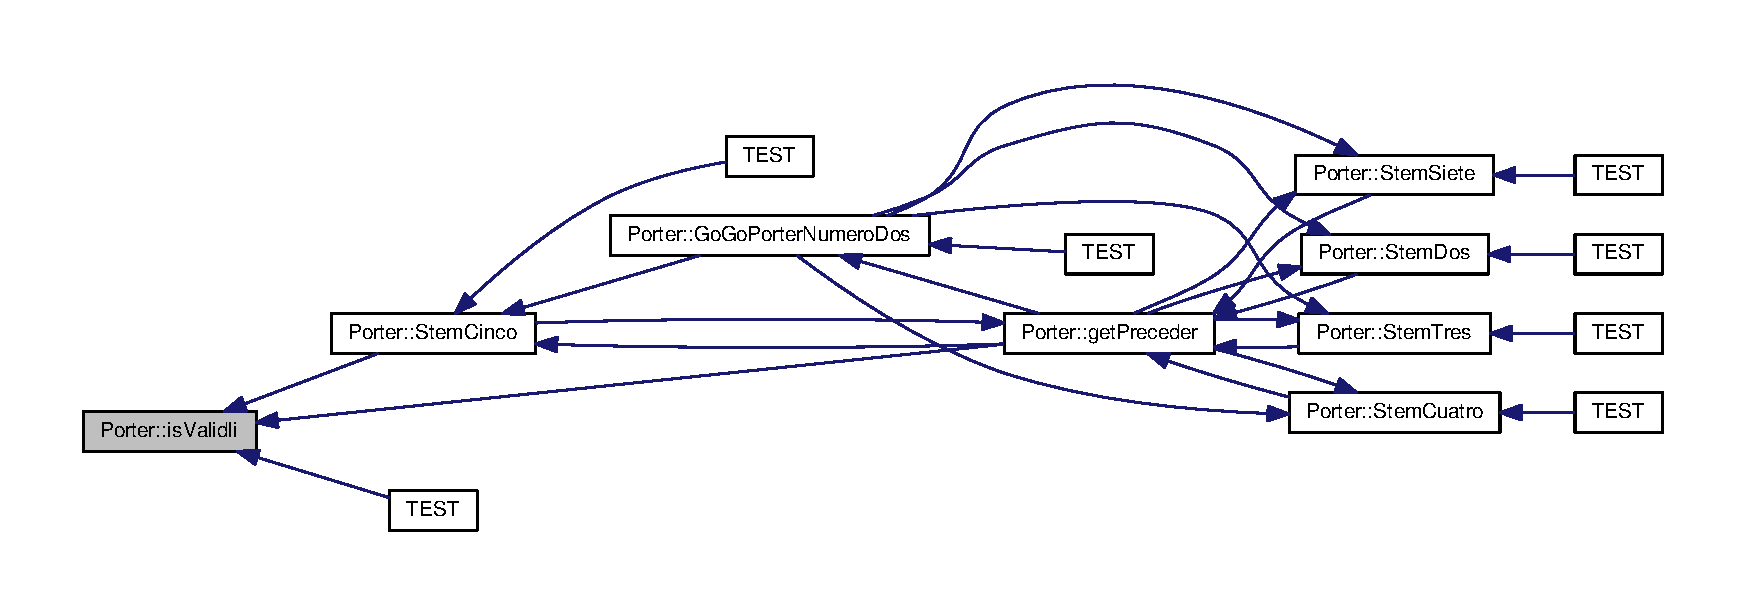
\includegraphics[width=350pt]{class_porter_ac53ad85d5d3178b72178a4d89137b55e_icgraph}
\end{center}
\end{figure}
\mbox{\Hypertarget{class_porter_ab16d2762c47b86b9a161be3d2c44203e}\label{class_porter_ab16d2762c47b86b9a161be3d2c44203e}} 
\index{Porter@{Porter}!is\+Vowel@{is\+Vowel}}
\index{is\+Vowel@{is\+Vowel}!Porter@{Porter}}
\subsubsection{\texorpdfstring{is\+Vowel()}{isVowel()}}
{\footnotesize\ttfamily bool Porter\+::is\+Vowel (\begin{DoxyParamCaption}\item[{const string \&}]{str,  }\item[{unsigned long long}]{loc }\end{DoxyParamCaption}) const}

is\+Vowel(str, int) Takes a string and a location of a char checks to see if said char is a vowel all other chars return false Here is the caller graph for this function\+:
\nopagebreak
\begin{figure}[H]
\begin{center}
\leavevmode
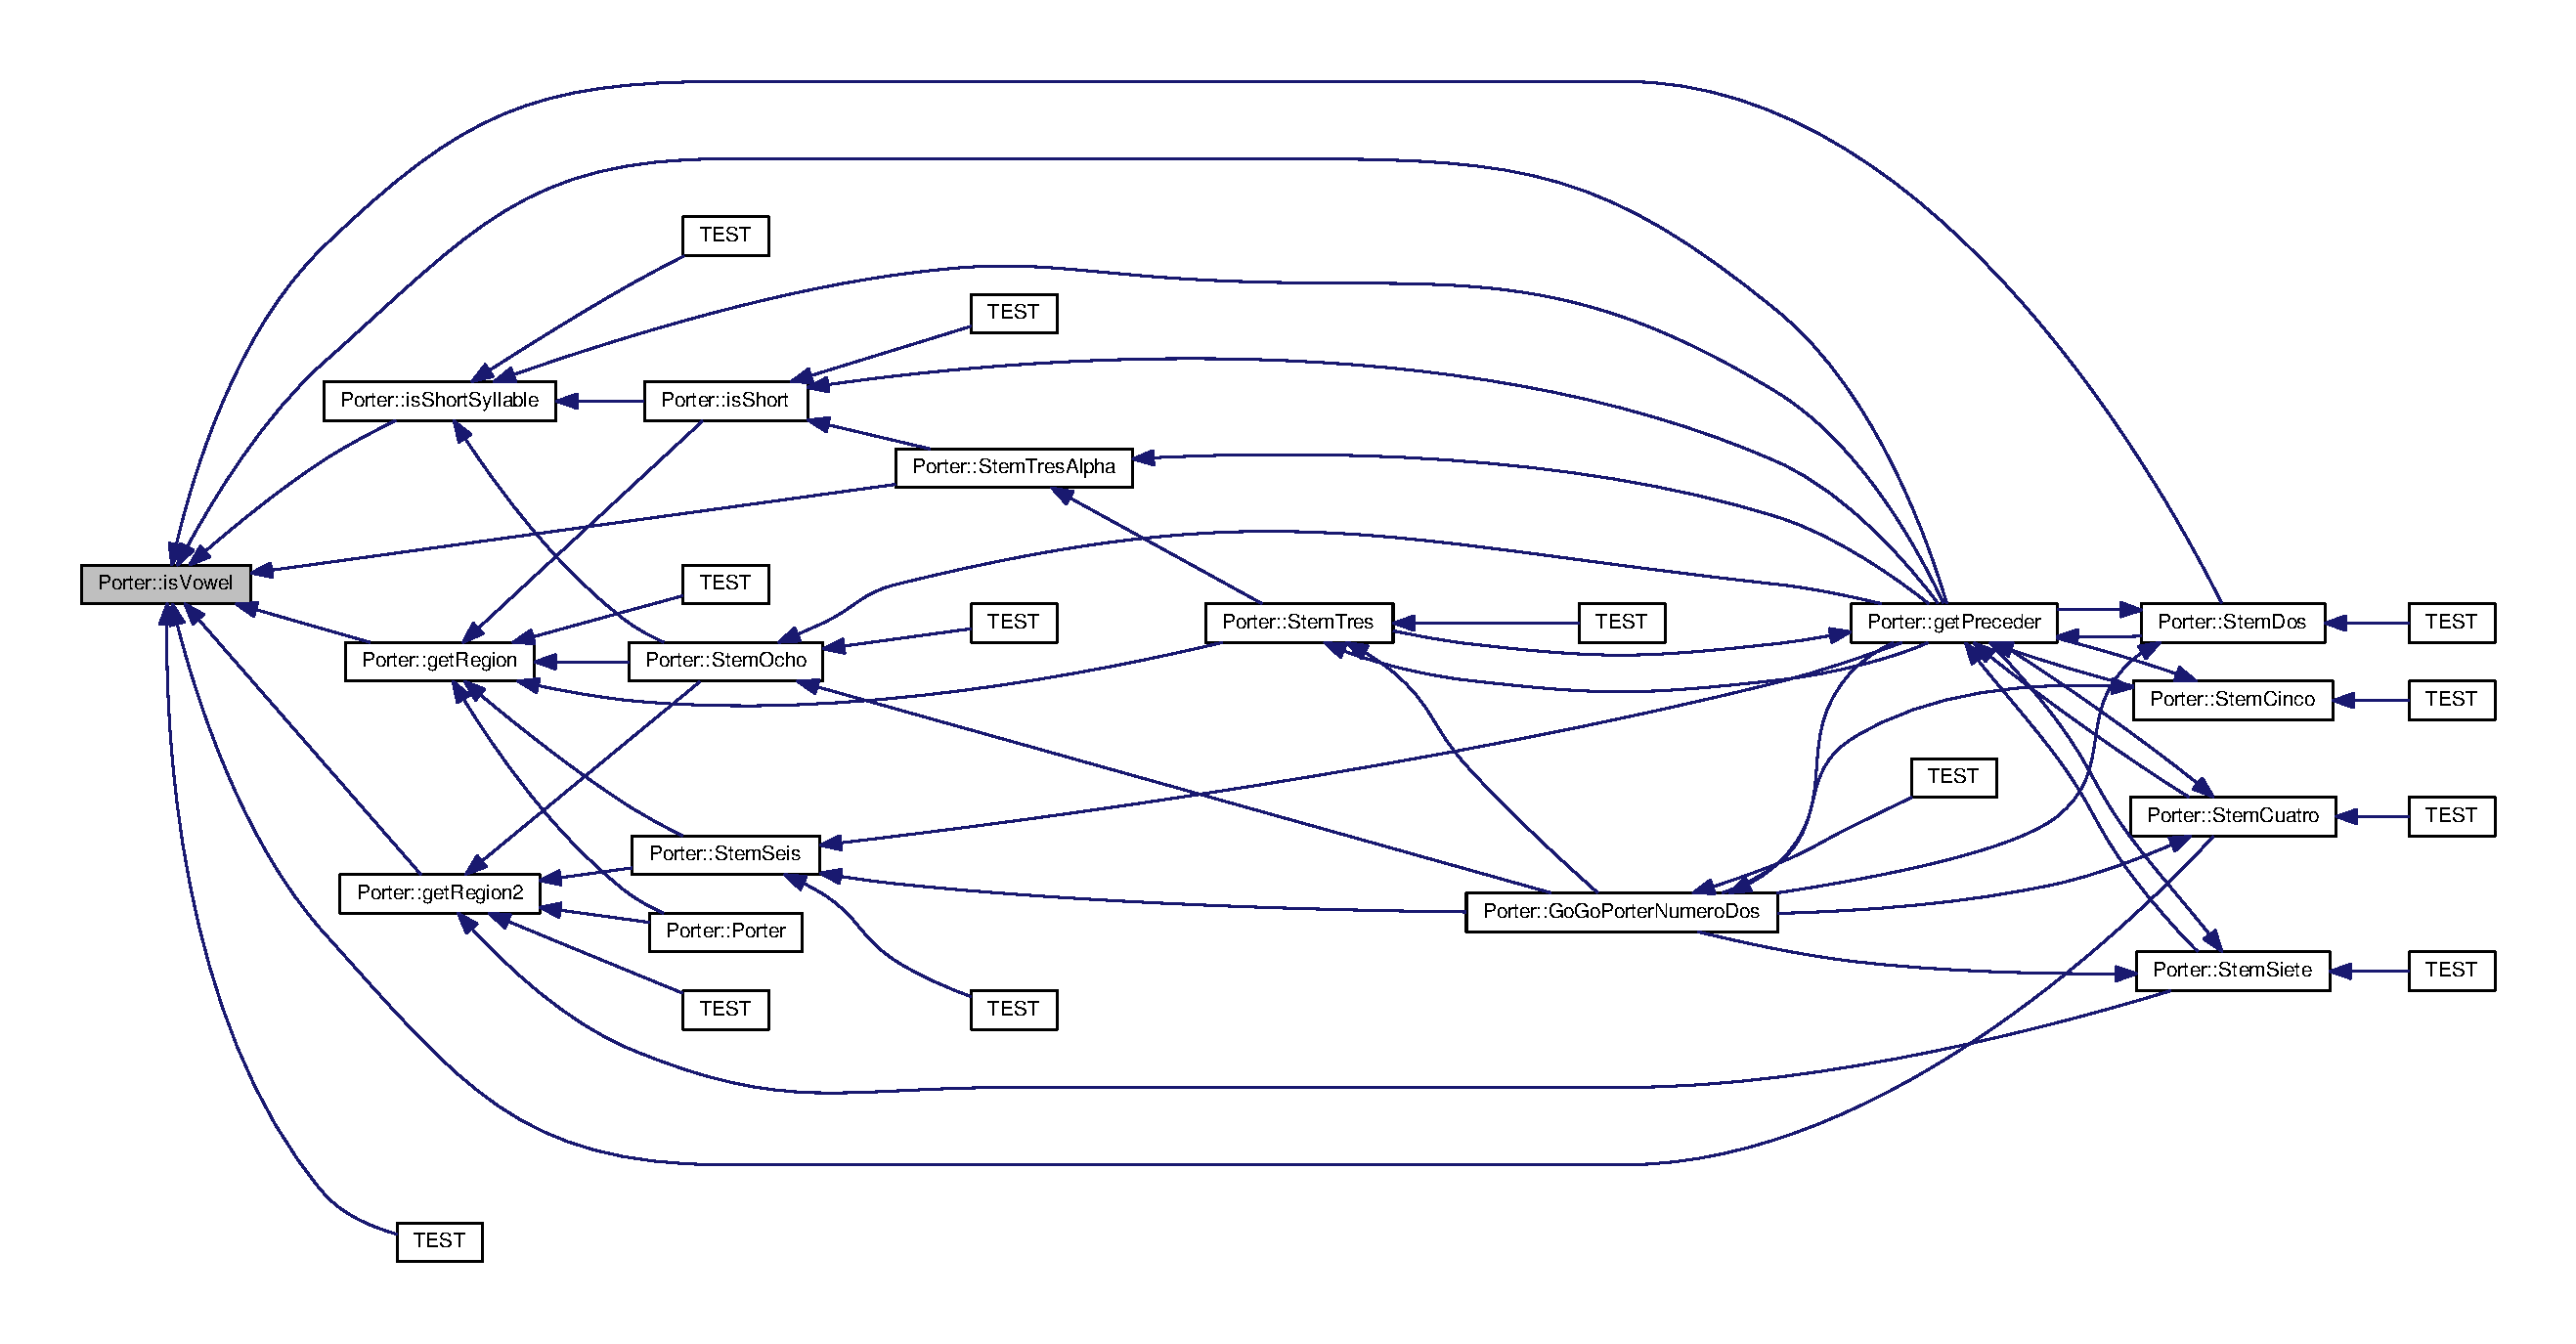
\includegraphics[width=350pt]{class_porter_ab16d2762c47b86b9a161be3d2c44203e_icgraph}
\end{center}
\end{figure}
\mbox{\Hypertarget{class_porter_aba12641d0e612b264097a35e4f2ffb45}\label{class_porter_aba12641d0e612b264097a35e4f2ffb45}} 
\index{Porter@{Porter}!replace@{replace}}
\index{replace@{replace}!Porter@{Porter}}
\subsubsection{\texorpdfstring{replace()}{replace()}}
{\footnotesize\ttfamily void Porter\+::replace (\begin{DoxyParamCaption}\item[{string \&}]{str,  }\item[{const string}]{replacement,  }\item[{const int}]{length }\end{DoxyParamCaption}) const}

replace method input\+: string, replacement, length returns string with replacement at length expects 0 $<$= length $<$= str.\+size() Here is the caller graph for this function\+:
\nopagebreak
\begin{figure}[H]
\begin{center}
\leavevmode
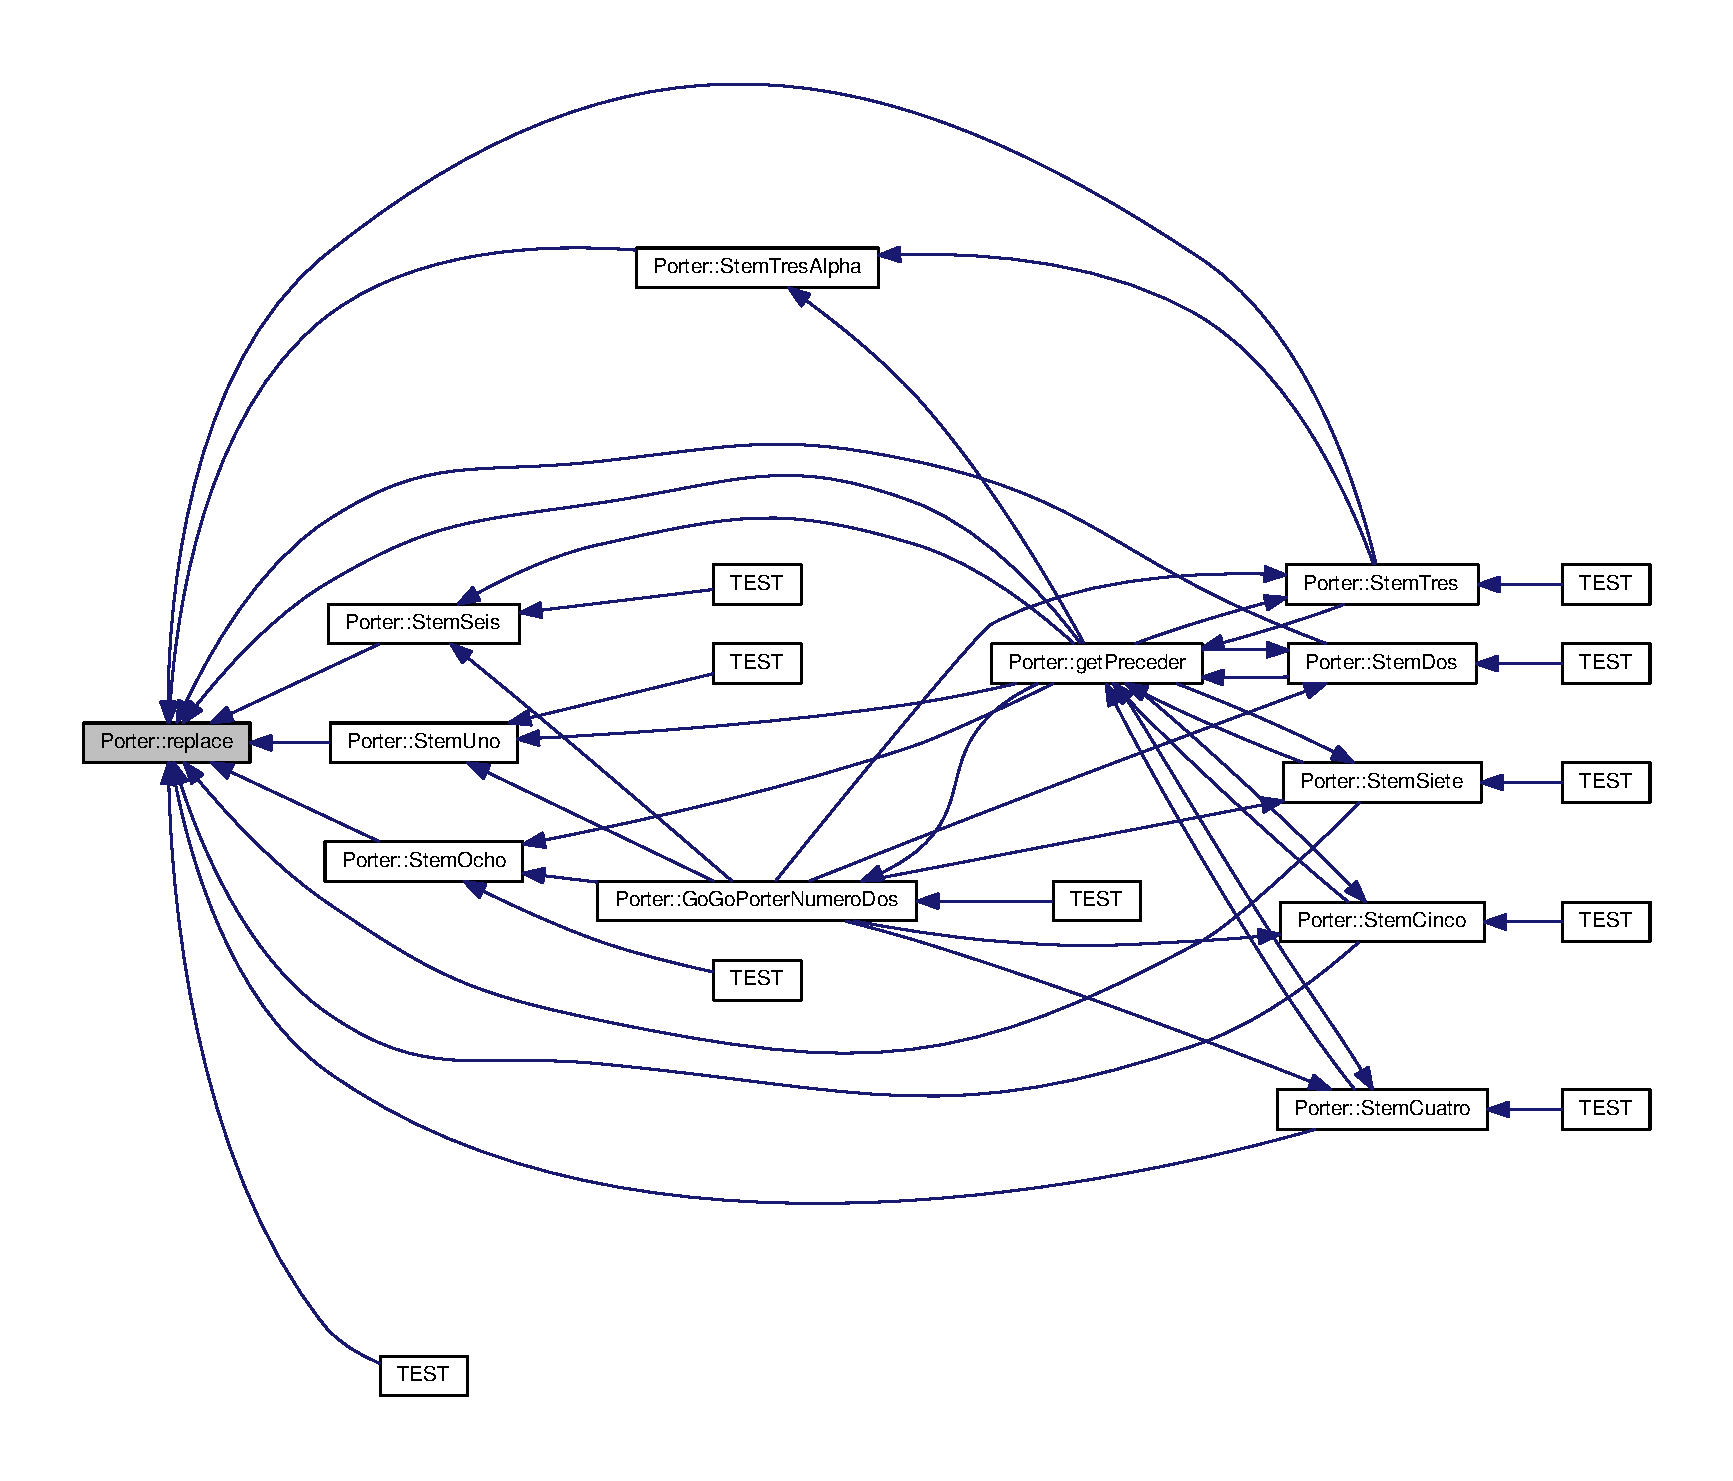
\includegraphics[width=350pt]{class_porter_aba12641d0e612b264097a35e4f2ffb45_icgraph}
\end{center}
\end{figure}
\mbox{\Hypertarget{class_porter_a916f45b55a1bbdaff7ce1db3d9a42813}\label{class_porter_a916f45b55a1bbdaff7ce1db3d9a42813}} 
\index{Porter@{Porter}!Stem\+Cinco@{Stem\+Cinco}}
\index{Stem\+Cinco@{Stem\+Cinco}!Porter@{Porter}}
\subsubsection{\texorpdfstring{Stem\+Cinco()}{StemCinco()}}
{\footnotesize\ttfamily void Porter\+::\+Stem\+Cinco (\begin{DoxyParamCaption}\item[{string \&}]{str,  }\item[{const unsigned long long}]{size }\end{DoxyParamCaption}) const}

Stem\+Cinco(str, int) Step \#5 of the \hyperlink{class_porter}{Porter} Algorithm Takes a string and its size and parses off\+: \{\char`\"{}ization\char`\"{}, \char`\"{}ational\char`\"{}, \char`\"{}fulness\char`\"{}, \char`\"{}ousness\char`\"{}, \char`\"{}iveness\char`\"{}, \char`\"{}tional\char`\"{}, \char`\"{}biliti\char`\"{}, \char`\"{}lessli\char`\"{}, \char`\"{}entli\char`\"{}, \char`\"{}ation\char`\"{}, \char`\"{}alism\char`\"{}, \char`\"{}aliti\char`\"{}, \char`\"{}ousli\char`\"{}, \char`\"{}iviti\char`\"{}, \char`\"{}fulli\char`\"{}, \char`\"{}enci\char`\"{}, \char`\"{}anci\char`\"{}, \char`\"{}abli\char`\"{}, \char`\"{}izer\char`\"{}, \char`\"{}ator\char`\"{}, \char`\"{}alli\char`\"{}, \char`\"{}bli\char`\"{}, \char`\"{}ogi\char`\"{}, \char`\"{}li\char`\"{}\} phew! Here is the call graph for this function\+:
\nopagebreak
\begin{figure}[H]
\begin{center}
\leavevmode
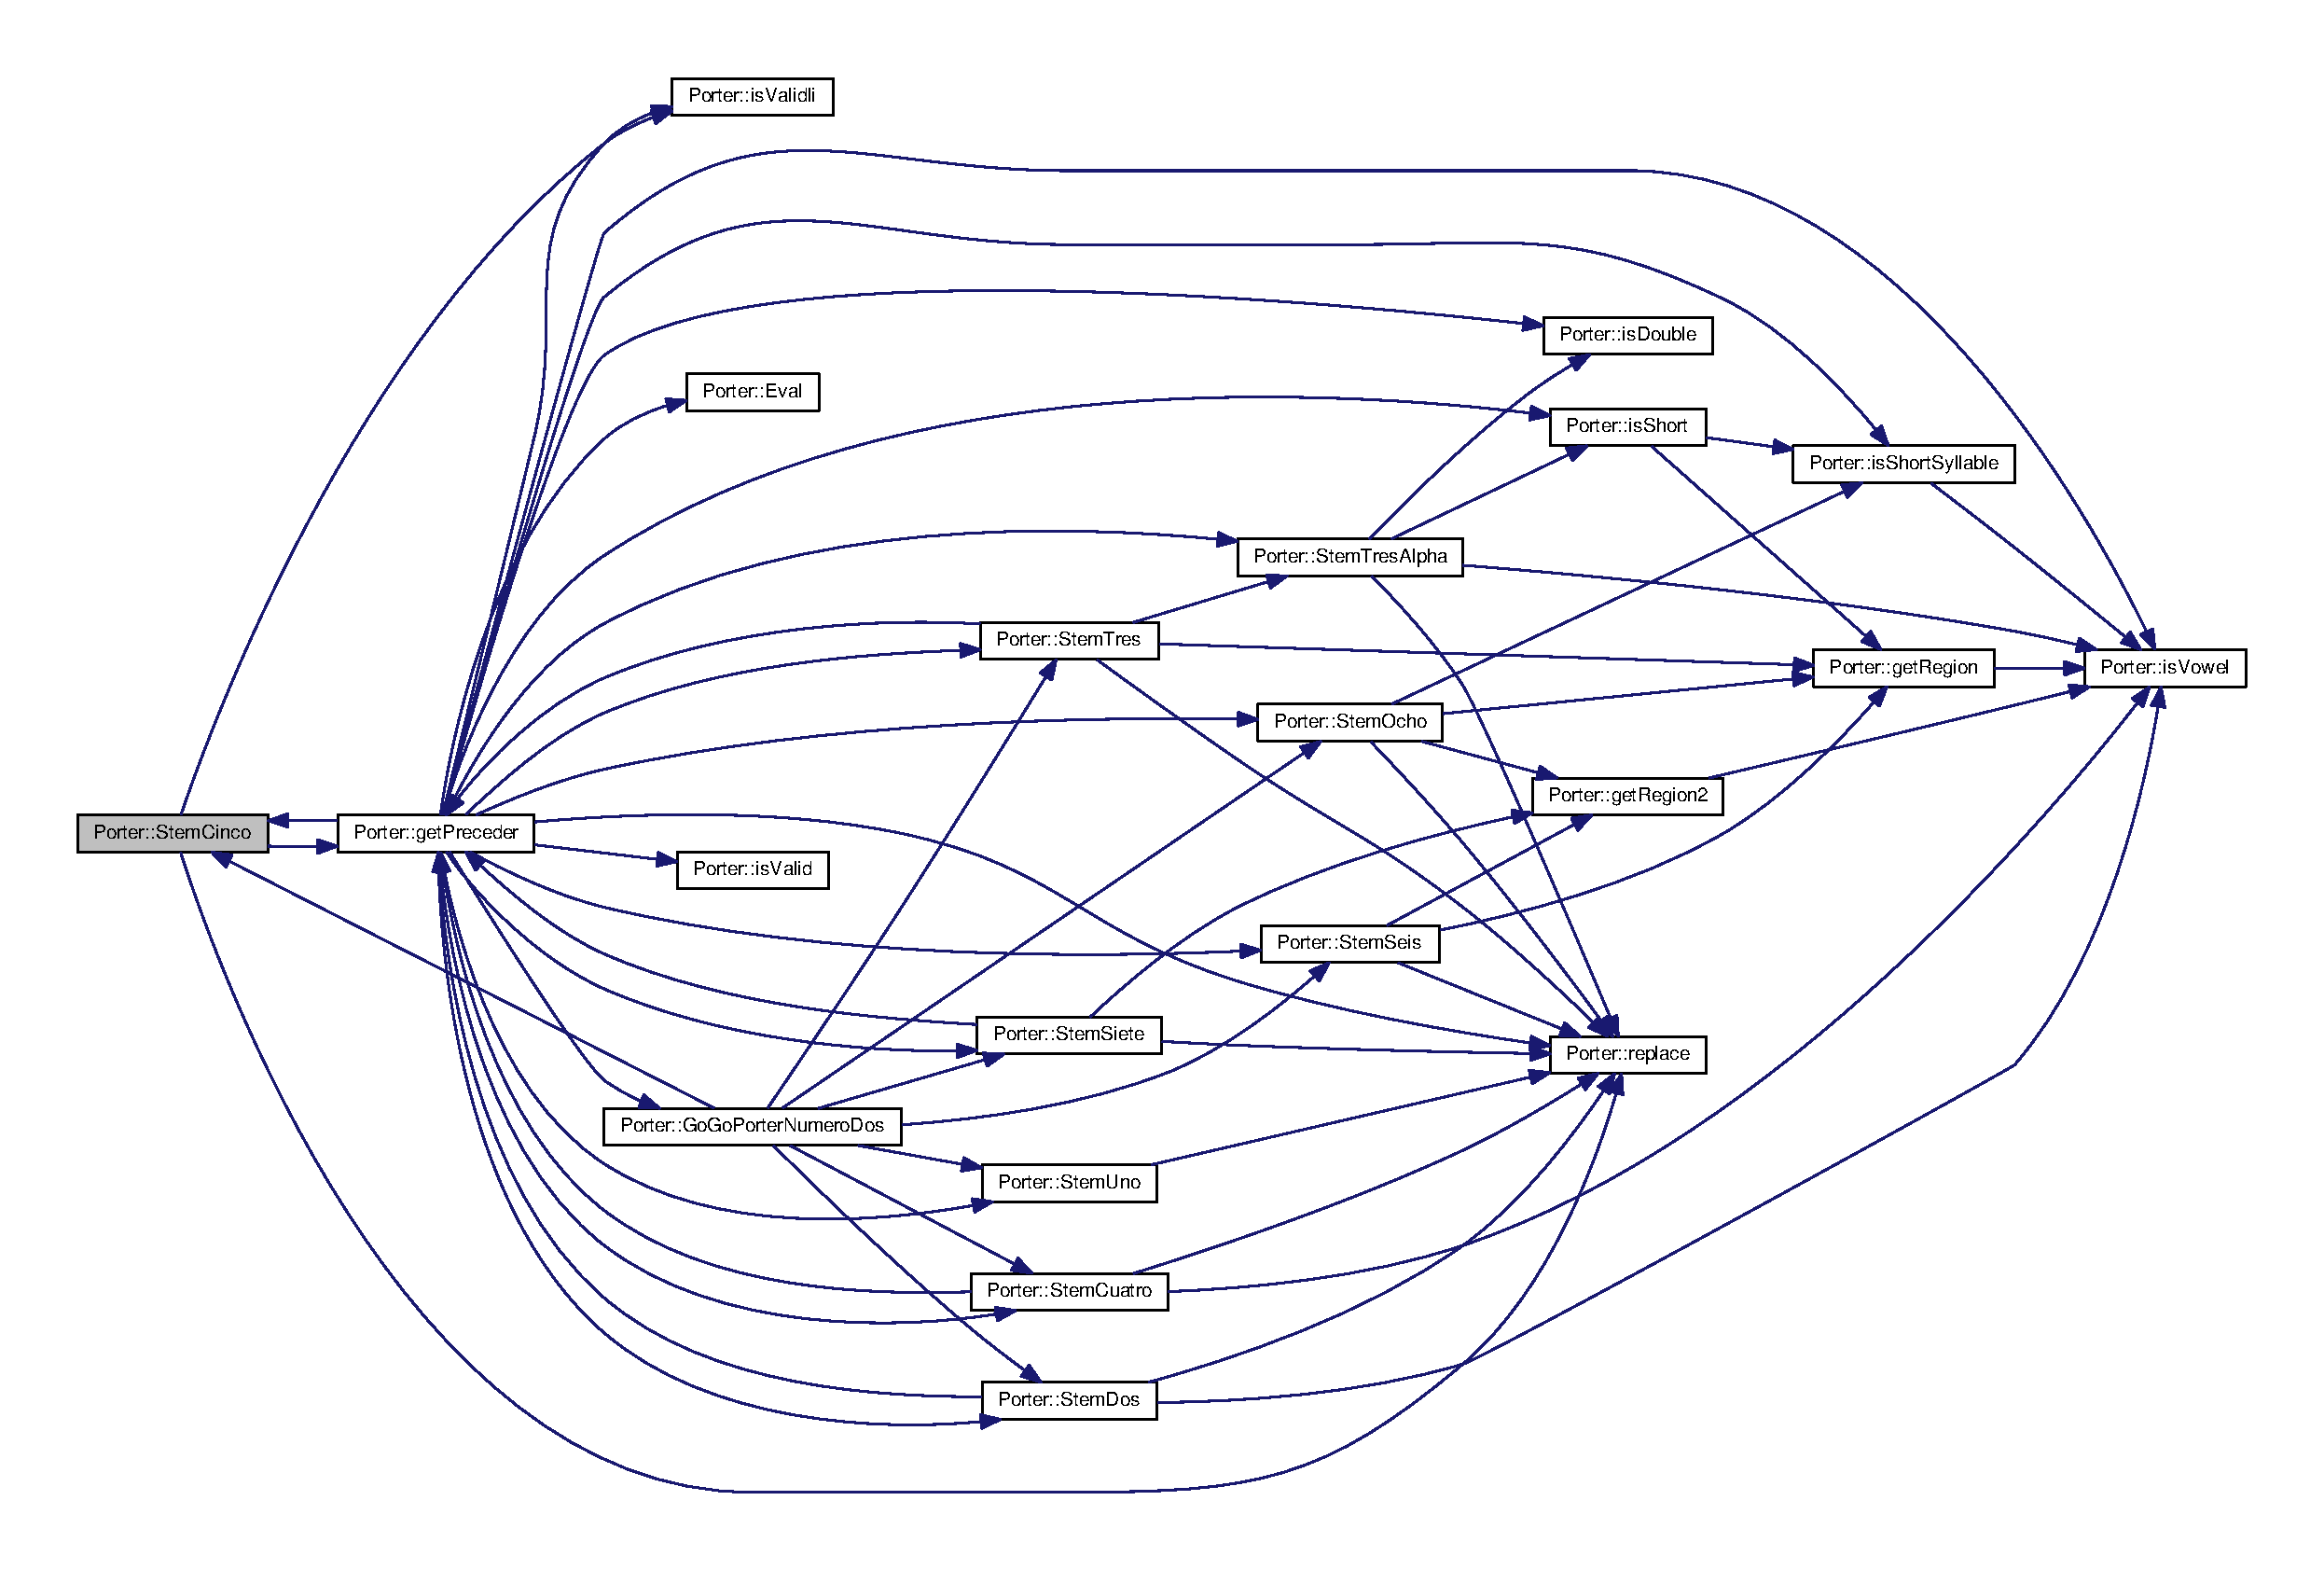
\includegraphics[width=350pt]{class_porter_a916f45b55a1bbdaff7ce1db3d9a42813_cgraph}
\end{center}
\end{figure}
Here is the caller graph for this function\+:
\nopagebreak
\begin{figure}[H]
\begin{center}
\leavevmode
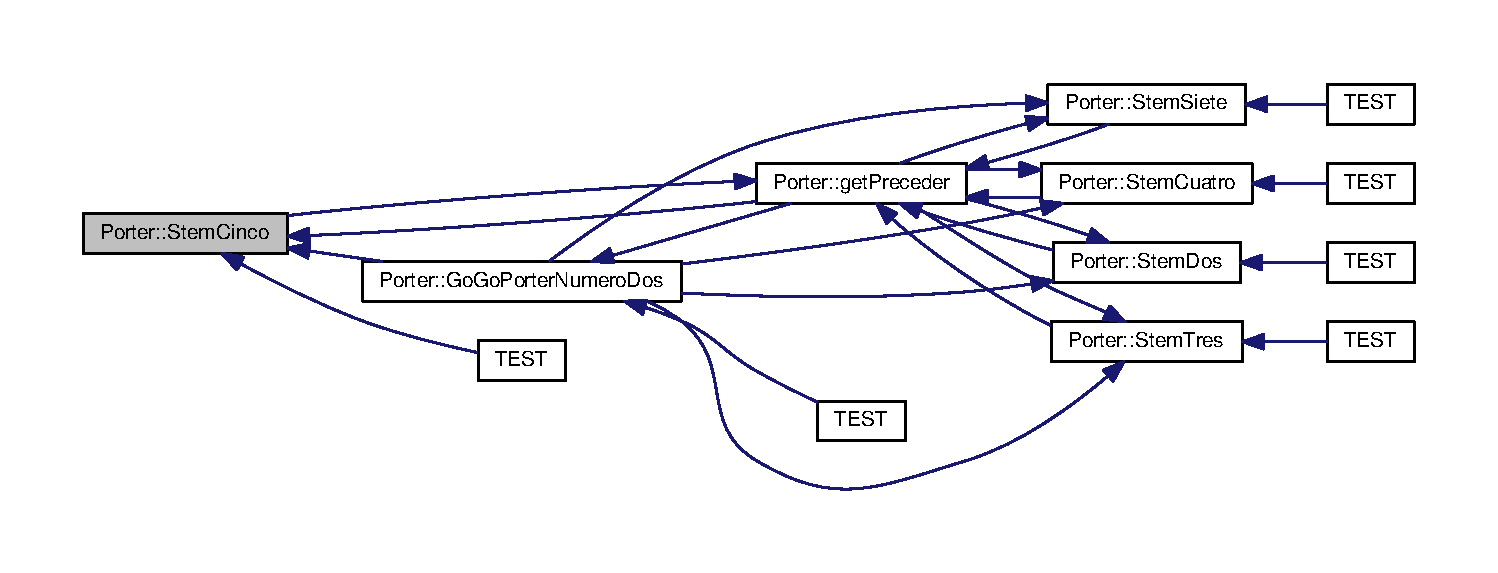
\includegraphics[width=350pt]{class_porter_a916f45b55a1bbdaff7ce1db3d9a42813_icgraph}
\end{center}
\end{figure}
\mbox{\Hypertarget{class_porter_aa1e1b416311f37b827bc093bb03ca500}\label{class_porter_aa1e1b416311f37b827bc093bb03ca500}} 
\index{Porter@{Porter}!Stem\+Cuatro@{Stem\+Cuatro}}
\index{Stem\+Cuatro@{Stem\+Cuatro}!Porter@{Porter}}
\subsubsection{\texorpdfstring{Stem\+Cuatro()}{StemCuatro()}}
{\footnotesize\ttfamily void Porter\+::\+Stem\+Cuatro (\begin{DoxyParamCaption}\item[{string \&}]{str,  }\item[{const unsigned long long}]{size }\end{DoxyParamCaption}) const}

Stem\+Cuatro(str, int) Step \#4 of the \hyperlink{class_porter}{Porter} Algorithm Takes a string and its size and parses off\+: \{\char`\"{}y\char`\"{}\} Here is the call graph for this function\+:
\nopagebreak
\begin{figure}[H]
\begin{center}
\leavevmode
\includegraphics[width=350pt]{class_porter_aa1e1b416311f37b827bc093bb03ca500_cgraph}
\end{center}
\end{figure}
Here is the caller graph for this function\+:
\nopagebreak
\begin{figure}[H]
\begin{center}
\leavevmode
\includegraphics[width=350pt]{class_porter_aa1e1b416311f37b827bc093bb03ca500_icgraph}
\end{center}
\end{figure}
\mbox{\Hypertarget{class_porter_a33838d3b5ab4963106a5c47c4a0c74e6}\label{class_porter_a33838d3b5ab4963106a5c47c4a0c74e6}} 
\index{Porter@{Porter}!Stem\+Dos@{Stem\+Dos}}
\index{Stem\+Dos@{Stem\+Dos}!Porter@{Porter}}
\subsubsection{\texorpdfstring{Stem\+Dos()}{StemDos()}}
{\footnotesize\ttfamily void Porter\+::\+Stem\+Dos (\begin{DoxyParamCaption}\item[{string \&}]{str,  }\item[{const unsigned long long}]{size }\end{DoxyParamCaption}) const}

Stem\+Dos(string) Step \#2 of the \hyperlink{class_porter}{Porter} Algorithm \{\char`\"{}sses\char`\"{}, \char`\"{}ies\char`\"{}, \char`\"{}ied\char`\"{}, \char`\"{}us\char`\"{}, \char`\"{}ss\char`\"{}, \char`\"{}s\char`\"{}\} Find the longest suffix that matches ... Here is the call graph for this function\+:
\nopagebreak
\begin{figure}[H]
\begin{center}
\leavevmode
\includegraphics[width=350pt]{class_porter_a33838d3b5ab4963106a5c47c4a0c74e6_cgraph}
\end{center}
\end{figure}
Here is the caller graph for this function\+:
\nopagebreak
\begin{figure}[H]
\begin{center}
\leavevmode
\includegraphics[width=350pt]{class_porter_a33838d3b5ab4963106a5c47c4a0c74e6_icgraph}
\end{center}
\end{figure}
\mbox{\Hypertarget{class_porter_a61853073641e47863fc6a85c786d8737}\label{class_porter_a61853073641e47863fc6a85c786d8737}} 
\index{Porter@{Porter}!Stem\+Ocho@{Stem\+Ocho}}
\index{Stem\+Ocho@{Stem\+Ocho}!Porter@{Porter}}
\subsubsection{\texorpdfstring{Stem\+Ocho()}{StemOcho()}}
{\footnotesize\ttfamily void Porter\+::\+Stem\+Ocho (\begin{DoxyParamCaption}\item[{string \&}]{str,  }\item[{const unsigned long long}]{size }\end{DoxyParamCaption}) const}

Stem\+Ocho(str, int) Step \#8 of the \hyperlink{class_porter}{Porter} Algorithm Takes a string and its size and parses off\+: \{\char`\"{}e\char`\"{}, \char`\"{}l\char`\"{}\} Here is the call graph for this function\+:
\nopagebreak
\begin{figure}[H]
\begin{center}
\leavevmode
\includegraphics[width=350pt]{class_porter_a61853073641e47863fc6a85c786d8737_cgraph}
\end{center}
\end{figure}
Here is the caller graph for this function\+:
\nopagebreak
\begin{figure}[H]
\begin{center}
\leavevmode
\includegraphics[width=350pt]{class_porter_a61853073641e47863fc6a85c786d8737_icgraph}
\end{center}
\end{figure}
\mbox{\Hypertarget{class_porter_a485f69d6797fce65144e0596f3190c2d}\label{class_porter_a485f69d6797fce65144e0596f3190c2d}} 
\index{Porter@{Porter}!Stem\+Seis@{Stem\+Seis}}
\index{Stem\+Seis@{Stem\+Seis}!Porter@{Porter}}
\subsubsection{\texorpdfstring{Stem\+Seis()}{StemSeis()}}
{\footnotesize\ttfamily void Porter\+::\+Stem\+Seis (\begin{DoxyParamCaption}\item[{string \&}]{str,  }\item[{const unsigned long long}]{size }\end{DoxyParamCaption}) const}

Stem\+Seis(str, int) Step \#6 of the \hyperlink{class_porter}{Porter} Algorithm Takes a string and its size and parses off\+: \{\char`\"{}ational\char`\"{}, \char`\"{}tional\char`\"{}, \char`\"{}alize\char`\"{}, \char`\"{}ative\char`\"{}, \char`\"{}icate\char`\"{}, \char`\"{}iciti\char`\"{}, \char`\"{}ical\char`\"{}, \char`\"{}ness\char`\"{}, \char`\"{}ful\char`\"{}\} Here is the call graph for this function\+:
\nopagebreak
\begin{figure}[H]
\begin{center}
\leavevmode
\includegraphics[width=350pt]{class_porter_a485f69d6797fce65144e0596f3190c2d_cgraph}
\end{center}
\end{figure}
Here is the caller graph for this function\+:
\nopagebreak
\begin{figure}[H]
\begin{center}
\leavevmode
\includegraphics[width=350pt]{class_porter_a485f69d6797fce65144e0596f3190c2d_icgraph}
\end{center}
\end{figure}
\mbox{\Hypertarget{class_porter_a1015f959403c55d740fff435f0cae439}\label{class_porter_a1015f959403c55d740fff435f0cae439}} 
\index{Porter@{Porter}!Stem\+Siete@{Stem\+Siete}}
\index{Stem\+Siete@{Stem\+Siete}!Porter@{Porter}}
\subsubsection{\texorpdfstring{Stem\+Siete()}{StemSiete()}}
{\footnotesize\ttfamily void Porter\+::\+Stem\+Siete (\begin{DoxyParamCaption}\item[{string \&}]{str,  }\item[{const unsigned long long}]{size }\end{DoxyParamCaption}) const}

Stem\+Siete(str, int) Step \#7 of the \hyperlink{class_porter}{Porter} Algorithm Takes a string and its size and parses off\+: \{\char`\"{}ement\char`\"{}, \char`\"{}ance\char`\"{}, \char`\"{}ence\char`\"{}, \char`\"{}able\char`\"{}, \char`\"{}ible\char`\"{}, \char`\"{}ment\char`\"{}, \char`\"{}ant\char`\"{}, \char`\"{}ent\char`\"{}, \char`\"{}ism\char`\"{}, \char`\"{}ate\char`\"{}, \char`\"{}iti\char`\"{}, \char`\"{}ous\char`\"{}, \char`\"{}ive\char`\"{}, \char`\"{}ize\char`\"{}, \char`\"{}ion\char`\"{}, \char`\"{}al\char`\"{}, \char`\"{}er\char`\"{}, \char`\"{}ic\char`\"{}\} Here is the call graph for this function\+:
\nopagebreak
\begin{figure}[H]
\begin{center}
\leavevmode
\includegraphics[width=350pt]{class_porter_a1015f959403c55d740fff435f0cae439_cgraph}
\end{center}
\end{figure}
Here is the caller graph for this function\+:
\nopagebreak
\begin{figure}[H]
\begin{center}
\leavevmode
\includegraphics[width=350pt]{class_porter_a1015f959403c55d740fff435f0cae439_icgraph}
\end{center}
\end{figure}
\mbox{\Hypertarget{class_porter_a4aadb1440bc5f143aba28641cab26ff6}\label{class_porter_a4aadb1440bc5f143aba28641cab26ff6}} 
\index{Porter@{Porter}!Stem\+Tres@{Stem\+Tres}}
\index{Stem\+Tres@{Stem\+Tres}!Porter@{Porter}}
\subsubsection{\texorpdfstring{Stem\+Tres()}{StemTres()}}
{\footnotesize\ttfamily void Porter\+::\+Stem\+Tres (\begin{DoxyParamCaption}\item[{string \&}]{str,  }\item[{const unsigned long long}]{size }\end{DoxyParamCaption}) const}

Stem\+Tres(str, int) Step \#3 of the \hyperlink{class_porter}{Porter} Algorithm Takes a string and its size and parses off\+: \{\char`\"{}eed\char`\"{}, \char`\"{}eedly\char`\"{}, \char`\"{}ed\char`\"{}, \char`\"{}edly\char`\"{}, \char`\"{}ing\char`\"{}, \char`\"{}ingly\char`\"{}\} Find the longest suffix that matches ... Here is the call graph for this function\+:
\nopagebreak
\begin{figure}[H]
\begin{center}
\leavevmode
\includegraphics[width=350pt]{class_porter_a4aadb1440bc5f143aba28641cab26ff6_cgraph}
\end{center}
\end{figure}
Here is the caller graph for this function\+:
\nopagebreak
\begin{figure}[H]
\begin{center}
\leavevmode
\includegraphics[width=350pt]{class_porter_a4aadb1440bc5f143aba28641cab26ff6_icgraph}
\end{center}
\end{figure}
\mbox{\Hypertarget{class_porter_ac5e4f3909a27316c6997c92a0019eaaf}\label{class_porter_ac5e4f3909a27316c6997c92a0019eaaf}} 
\index{Porter@{Porter}!Stem\+Tres\+Alpha@{Stem\+Tres\+Alpha}}
\index{Stem\+Tres\+Alpha@{Stem\+Tres\+Alpha}!Porter@{Porter}}
\subsubsection{\texorpdfstring{Stem\+Tres\+Alpha()}{StemTresAlpha()}}
{\footnotesize\ttfamily void Porter\+::\+Stem\+Tres\+Alpha (\begin{DoxyParamCaption}\item[{string \&}]{str,  }\item[{const string \&}]{preceder,  }\item[{const unsigned long long}]{length }\end{DoxyParamCaption}) const}

Stem\+Tres\+Alpha(str, int) Takes a string and a length this particular case repeats a lot of requiremnts and it has some aditional special requirements that have to be checked after replacing the suffix This alpha function takes care all of that, rather than copy + pasta everywhere Special Requirements\+: 1) if preceder ends in \{\char`\"{}at\char`\"{}, \char`\"{}bl\char`\"{}, \char`\"{}iz\char`\"{}\} 2) if preceder \hyperlink{class_porter_a7c8a4b3b6103ce655e8ffc8a3eba1897}{is\+Double()} 3) if preceder \hyperlink{class_porter_a35b1cc5606d4e78d1f69ac4037fdde87}{is\+Short()} Here is the call graph for this function\+:
\nopagebreak
\begin{figure}[H]
\begin{center}
\leavevmode
\includegraphics[width=350pt]{class_porter_ac5e4f3909a27316c6997c92a0019eaaf_cgraph}
\end{center}
\end{figure}
Here is the caller graph for this function\+:
\nopagebreak
\begin{figure}[H]
\begin{center}
\leavevmode
\includegraphics[width=350pt]{class_porter_ac5e4f3909a27316c6997c92a0019eaaf_icgraph}
\end{center}
\end{figure}
\mbox{\Hypertarget{class_porter_ad8b63c9741655393ff9c849d269c953a}\label{class_porter_ad8b63c9741655393ff9c849d269c953a}} 
\index{Porter@{Porter}!Stem\+Uno@{Stem\+Uno}}
\index{Stem\+Uno@{Stem\+Uno}!Porter@{Porter}}
\subsubsection{\texorpdfstring{Stem\+Uno()}{StemUno()}}
{\footnotesize\ttfamily void Porter\+::\+Stem\+Uno (\begin{DoxyParamCaption}\item[{string \&}]{str,  }\item[{const unsigned long long}]{size }\end{DoxyParamCaption}) const}

Stem\+Uno(string) Step \#1 of the \hyperlink{class_porter}{Porter} Algorithm \{\char`\"{}\textquotesingle{}s\textquotesingle{}\char`\"{}, \char`\"{}\textquotesingle{}s\char`\"{}, \char`\"{}\textquotesingle{}\char`\"{}\} and any one leading \char`\"{}\textquotesingle{}\char`\"{} Find the longest suffix that matches the ending of the word If the conditions of the suffix are satisfied, remove the suffix and add the replacement. If the conditions of the suffix are N\+OT satisfied, do nothing Here is the call graph for this function\+:
\nopagebreak
\begin{figure}[H]
\begin{center}
\leavevmode
\includegraphics[width=286pt]{class_porter_ad8b63c9741655393ff9c849d269c953a_cgraph}
\end{center}
\end{figure}
Here is the caller graph for this function\+:
\nopagebreak
\begin{figure}[H]
\begin{center}
\leavevmode
\includegraphics[width=350pt]{class_porter_ad8b63c9741655393ff9c849d269c953a_icgraph}
\end{center}
\end{figure}


The documentation for this class was generated from the following files\+:\begin{DoxyCompactItemize}
\item 
\hyperlink{_porter_8h}{Porter.\+h}\item 
\hyperlink{_porter_8cpp}{Porter.\+cpp}\end{DoxyCompactItemize}

\chapter{File Documentation}
\hypertarget{_cluster_8cpp}{}\section{Cluster.\+cpp File Reference}
\label{_cluster_8cpp}\index{Cluster.\+cpp@{Cluster.\+cpp}}
{\ttfamily \#include \char`\"{}Cluster.\+h\char`\"{}}\newline
Include dependency graph for Cluster.\+cpp\+:
\nopagebreak
\begin{figure}[H]
\begin{center}
\leavevmode
\includegraphics[width=350pt]{_cluster_8cpp__incl}
\end{center}
\end{figure}
\subsection*{Functions}
\begin{DoxyCompactItemize}
\item 
std\+::ostream \& \hyperlink{_cluster_8cpp_a80e9d0c8af3d3700176af496cc2dcf29}{operator$<$$<$} (std\+::ostream \&out, const \hyperlink{class_cluster}{Cluster} \&c0)
\end{DoxyCompactItemize}


\subsection{Detailed Description}
\+: implements the \hyperlink{class_cluster}{Cluster} class 

\subsection{Function Documentation}
\mbox{\Hypertarget{_cluster_8cpp_a80e9d0c8af3d3700176af496cc2dcf29}\label{_cluster_8cpp_a80e9d0c8af3d3700176af496cc2dcf29}} 
\index{Cluster.\+cpp@{Cluster.\+cpp}!operator$<$$<$@{operator$<$$<$}}
\index{operator$<$$<$@{operator$<$$<$}!Cluster.\+cpp@{Cluster.\+cpp}}
\subsubsection{\texorpdfstring{operator$<$$<$()}{operator<<()}}
{\footnotesize\ttfamily std\+::ostream\& operator$<$$<$ (\begin{DoxyParamCaption}\item[{std\+::ostream \&}]{out,  }\item[{const \hyperlink{class_cluster}{Cluster} \&}]{c0 }\end{DoxyParamCaption})}

Here is the call graph for this function\+:
\nopagebreak
\begin{figure}[H]
\begin{center}
\leavevmode
\includegraphics[width=281pt]{_cluster_8cpp_a80e9d0c8af3d3700176af496cc2dcf29_cgraph}
\end{center}
\end{figure}

\hypertarget{_cluster_8h}{}\section{Cluster.\+h File Reference}
\label{_cluster_8h}\index{Cluster.\+h@{Cluster.\+h}}
{\ttfamily \#include $<$iostream$>$}\newline
{\ttfamily \#include $<$fstream$>$}\newline
{\ttfamily \#include $<$vector$>$}\newline
{\ttfamily \#include $<$string$>$}\newline
{\ttfamily \#include $<$unordered\+\_\+map$>$}\newline
{\ttfamily \#include $<$math.\+h$>$}\newline
{\ttfamily \#include \char`\"{}Histogram.\+h\char`\"{}}\newline
Include dependency graph for Cluster.\+h\+:
\nopagebreak
\begin{figure}[H]
\begin{center}
\leavevmode
\includegraphics[width=350pt]{_cluster_8h__incl}
\end{center}
\end{figure}
This graph shows which files directly or indirectly include this file\+:
\nopagebreak
\begin{figure}[H]
\begin{center}
\leavevmode
\includegraphics[width=222pt]{_cluster_8h__dep__incl}
\end{center}
\end{figure}
\subsection*{Classes}
\begin{DoxyCompactItemize}
\item 
class \hyperlink{class_cluster}{Cluster}
\begin{DoxyCompactList}\small\item\em A cluster of histograms for comparison. \end{DoxyCompactList}\end{DoxyCompactItemize}


\subsection{Detailed Description}
\+: Declares the \hyperlink{class_cluster}{Cluster} class 
\hypertarget{_coleman_liau_8cpp}{}\section{Coleman\+Liau.\+cpp File Reference}
\label{_coleman_liau_8cpp}\index{Coleman\+Liau.\+cpp@{Coleman\+Liau.\+cpp}}
{\ttfamily \#include $<$Coleman\+Liau.\+h$>$}\newline
Include dependency graph for Coleman\+Liau.\+cpp\+:
\nopagebreak
\begin{figure}[H]
\begin{center}
\leavevmode
\includegraphics[width=350pt]{_coleman_liau_8cpp__incl}
\end{center}
\end{figure}
\subsection*{Functions}
\begin{DoxyCompactItemize}
\item 
std\+::ostream \& \hyperlink{_coleman_liau_8cpp_a896867aacd954df4faecc74a7010a8b0}{operator$<$$<$} (std\+::ostream \&out, const \hyperlink{class_coleman_liau}{Coleman\+Liau} \&c0)
\end{DoxyCompactItemize}


\subsection{Detailed Description}
\+: implements the Coleman-\/\+Liau class 

\subsection{Function Documentation}
\mbox{\Hypertarget{_coleman_liau_8cpp_a896867aacd954df4faecc74a7010a8b0}\label{_coleman_liau_8cpp_a896867aacd954df4faecc74a7010a8b0}} 
\index{Coleman\+Liau.\+cpp@{Coleman\+Liau.\+cpp}!operator$<$$<$@{operator$<$$<$}}
\index{operator$<$$<$@{operator$<$$<$}!Coleman\+Liau.\+cpp@{Coleman\+Liau.\+cpp}}
\subsubsection{\texorpdfstring{operator$<$$<$()}{operator<<()}}
{\footnotesize\ttfamily std\+::ostream\& operator$<$$<$ (\begin{DoxyParamCaption}\item[{std\+::ostream \&}]{out,  }\item[{const \hyperlink{class_coleman_liau}{Coleman\+Liau} \&}]{c0 }\end{DoxyParamCaption})}

Here is the call graph for this function\+:
\nopagebreak
\begin{figure}[H]
\begin{center}
\leavevmode
\includegraphics[width=350pt]{_coleman_liau_8cpp_a896867aacd954df4faecc74a7010a8b0_cgraph}
\end{center}
\end{figure}

\hypertarget{_coleman_liau_8h}{}\section{Coleman\+Liau.\+h File Reference}
\label{_coleman_liau_8h}\index{Coleman\+Liau.\+h@{Coleman\+Liau.\+h}}
{\ttfamily \#include $<$Histogram.\+h$>$}\newline
{\ttfamily \#include $<$vector$>$}\newline
{\ttfamily \#include $<$string$>$}\newline
{\ttfamily \#include $<$cstddef$>$}\newline
Include dependency graph for Coleman\+Liau.\+h\+:
\nopagebreak
\begin{figure}[H]
\begin{center}
\leavevmode
\includegraphics[width=350pt]{_coleman_liau_8h__incl}
\end{center}
\end{figure}
This graph shows which files directly or indirectly include this file\+:
\nopagebreak
\begin{figure}[H]
\begin{center}
\leavevmode
\includegraphics[width=246pt]{_coleman_liau_8h__dep__incl}
\end{center}
\end{figure}
\subsection*{Classes}
\begin{DoxyCompactItemize}
\item 
class \hyperlink{class_coleman_liau}{Coleman\+Liau}
\begin{DoxyCompactList}\small\item\em An implementation of the Coleman-\/\+Liau index algorithm. \end{DoxyCompactList}\end{DoxyCompactItemize}


\subsection{Detailed Description}
\+: Declares the Coleman-\/\+Liau Index Algorithm class 
\hypertarget{_histogram_8cpp}{}\section{Histogram.\+cpp File Reference}
\label{_histogram_8cpp}\index{Histogram.\+cpp@{Histogram.\+cpp}}
{\ttfamily \#include $<$Histogram.\+h$>$}\newline
Include dependency graph for Histogram.\+cpp\+:
\nopagebreak
\begin{figure}[H]
\begin{center}
\leavevmode
\includegraphics[width=350pt]{_histogram_8cpp__incl}
\end{center}
\end{figure}


\subsection{Detailed Description}
\+: implements the \hyperlink{class_histogram}{Histogram} class 
\hypertarget{_histogram_8h}{}\section{Histogram.\+h File Reference}
\label{_histogram_8h}\index{Histogram.\+h@{Histogram.\+h}}
{\ttfamily \#include $<$iostream$>$}\newline
{\ttfamily \#include $<$fstream$>$}\newline
{\ttfamily \#include $<$sstream$>$}\newline
{\ttfamily \#include $<$vector$>$}\newline
{\ttfamily \#include $<$map$>$}\newline
{\ttfamily \#include $<$string$>$}\newline
{\ttfamily \#include $<$unordered\+\_\+map$>$}\newline
{\ttfamily \#include \char`\"{}Lexeme.\+h\char`\"{}}\newline
Include dependency graph for Histogram.\+h\+:
\nopagebreak
\begin{figure}[H]
\begin{center}
\leavevmode
\includegraphics[width=350pt]{_histogram_8h__incl}
\end{center}
\end{figure}
This graph shows which files directly or indirectly include this file\+:
\nopagebreak
\begin{figure}[H]
\begin{center}
\leavevmode
\includegraphics[width=350pt]{_histogram_8h__dep__incl}
\end{center}
\end{figure}
\subsection*{Classes}
\begin{DoxyCompactItemize}
\item 
class \hyperlink{class_histogram}{Histogram}
\begin{DoxyCompactList}\small\item\em A string histogram for simple counting (currently) \end{DoxyCompactList}\end{DoxyCompactItemize}


\subsection{Detailed Description}
\+: Declares the \hyperlink{class_histogram}{Histogram} class 
\hypertarget{_lexeme_8h}{}\section{Lexeme.\+h File Reference}
\label{_lexeme_8h}\index{Lexeme.\+h@{Lexeme.\+h}}
{\ttfamily \#include $<$string$>$}\newline
Include dependency graph for Lexeme.\+h\+:
\nopagebreak
\begin{figure}[H]
\begin{center}
\leavevmode
\includegraphics[width=139pt]{_lexeme_8h__incl}
\end{center}
\end{figure}
This graph shows which files directly or indirectly include this file\+:
\nopagebreak
\begin{figure}[H]
\begin{center}
\leavevmode
\includegraphics[width=350pt]{_lexeme_8h__dep__incl}
\end{center}
\end{figure}
\subsection*{Classes}
\begin{DoxyCompactItemize}
\item 
class \hyperlink{class_lexeme}{Lexeme}
\begin{DoxyCompactList}\small\item\em An implementation of a lexeme (word) \end{DoxyCompactList}\end{DoxyCompactItemize}


\subsection{Detailed Description}
\+: Declares the \hyperlink{class_lexeme}{Lexeme} class 
\hypertarget{main_8cpp}{}\section{main.\+cpp File Reference}
\label{main_8cpp}\index{main.\+cpp@{main.\+cpp}}
{\ttfamily \#include $<$Cluster.\+h$>$}\newline
{\ttfamily \#include $<$Histogram.\+h$>$}\newline
{\ttfamily \#include $<$Porter.\+h$>$}\newline
{\ttfamily \#include $<$Coleman\+Liau.\+h$>$}\newline
{\ttfamily \#include $<$iostream$>$}\newline
{\ttfamily \#include $<$fstream$>$}\newline
Include dependency graph for main.\+cpp\+:
\nopagebreak
\begin{figure}[H]
\begin{center}
\leavevmode
\includegraphics[width=350pt]{main_8cpp__incl}
\end{center}
\end{figure}
\subsection*{Functions}
\begin{DoxyCompactItemize}
\item 
int \hyperlink{main_8cpp_a244fa59877f3cf7313b2bbb55a9876f0}{Usage} (char $\ast$arg0, const char $\ast$location)
\begin{DoxyCompactList}\small\item\em Print the correct usage in case of user syntax error. \end{DoxyCompactList}\item 
int \hyperlink{main_8cpp_a3c04138a5bfe5d72780bb7e82a18e627}{main} (int argc, char $\ast$$\ast$argv)
\end{DoxyCompactItemize}


\subsection{Detailed Description}
\+: main function for C\+S253 \hyperlink{class_histogram}{Histogram} (H\+W1) 

\subsection{Function Documentation}
\mbox{\Hypertarget{main_8cpp_a3c04138a5bfe5d72780bb7e82a18e627}\label{main_8cpp_a3c04138a5bfe5d72780bb7e82a18e627}} 
\index{main.\+cpp@{main.\+cpp}!main@{main}}
\index{main@{main}!main.\+cpp@{main.\+cpp}}
\subsubsection{\texorpdfstring{main()}{main()}}
{\footnotesize\ttfamily int main (\begin{DoxyParamCaption}\item[{int}]{argc,  }\item[{char $\ast$$\ast$}]{argv }\end{DoxyParamCaption})}

Here is the call graph for this function\+:
\nopagebreak
\begin{figure}[H]
\begin{center}
\leavevmode
\includegraphics[width=350pt]{main_8cpp_a3c04138a5bfe5d72780bb7e82a18e627_cgraph}
\end{center}
\end{figure}
\mbox{\Hypertarget{main_8cpp_a244fa59877f3cf7313b2bbb55a9876f0}\label{main_8cpp_a244fa59877f3cf7313b2bbb55a9876f0}} 
\index{main.\+cpp@{main.\+cpp}!Usage@{Usage}}
\index{Usage@{Usage}!main.\+cpp@{main.\+cpp}}
\subsubsection{\texorpdfstring{Usage()}{Usage()}}
{\footnotesize\ttfamily int Usage (\begin{DoxyParamCaption}\item[{char $\ast$}]{arg0,  }\item[{const char $\ast$}]{location }\end{DoxyParamCaption})}



Print the correct usage in case of user syntax error. 

Here is the caller graph for this function\+:
\nopagebreak
\begin{figure}[H]
\begin{center}
\leavevmode
\includegraphics[width=199pt]{main_8cpp_a244fa59877f3cf7313b2bbb55a9876f0_icgraph}
\end{center}
\end{figure}

\hypertarget{_porter_8cpp}{}\section{Porter.\+cpp File Reference}
\label{_porter_8cpp}\index{Porter.\+cpp@{Porter.\+cpp}}
{\ttfamily \#include $<$Porter.\+h$>$}\newline
Include dependency graph for Porter.\+cpp\+:
\nopagebreak
\begin{figure}[H]
\begin{center}
\leavevmode
\includegraphics[width=350pt]{_porter_8cpp__incl}
\end{center}
\end{figure}


\subsection{Detailed Description}
\+: implements the \hyperlink{class_porter}{Porter} class 
\hypertarget{_porter_8h}{}\section{Porter.\+h File Reference}
\label{_porter_8h}\index{Porter.\+h@{Porter.\+h}}
{\ttfamily \#include $<$Histogram.\+h$>$}\newline
{\ttfamily \#include $<$vector$>$}\newline
{\ttfamily \#include $<$string$>$}\newline
{\ttfamily \#include $<$cstddef$>$}\newline
Include dependency graph for Porter.\+h\+:
\nopagebreak
\begin{figure}[H]
\begin{center}
\leavevmode
\includegraphics[width=350pt]{_porter_8h__incl}
\end{center}
\end{figure}
This graph shows which files directly or indirectly include this file\+:
\nopagebreak
\begin{figure}[H]
\begin{center}
\leavevmode
\includegraphics[width=320pt]{_porter_8h__dep__incl}
\end{center}
\end{figure}
\subsection*{Classes}
\begin{DoxyCompactItemize}
\item 
class \hyperlink{class_porter}{Porter}
\begin{DoxyCompactList}\small\item\em An implementation of the \hyperlink{class_porter}{Porter} Algorithm \#2. \end{DoxyCompactList}\end{DoxyCompactItemize}


\subsection{Detailed Description}
\+: Declares the \hyperlink{class_porter}{Porter} Algorithm class 
\hypertarget{porter_tests_8cpp}{}\section{porter\+Tests.\+cpp File Reference}
\label{porter_tests_8cpp}\index{porter\+Tests.\+cpp@{porter\+Tests.\+cpp}}
{\ttfamily \#include \char`\"{}Histogram.\+h\char`\"{}}\newline
{\ttfamily \#include \char`\"{}Porter.\+h\char`\"{}}\newline
{\ttfamily \#include $<$limits.\+h$>$}\newline
{\ttfamily \#include $<$gtest/gtest.\+h$>$}\newline
Include dependency graph for porter\+Tests.\+cpp\+:
\nopagebreak
\begin{figure}[H]
\begin{center}
\leavevmode
\includegraphics[width=350pt]{porter_tests_8cpp__incl}
\end{center}
\end{figure}
\subsection*{Functions}
\begin{DoxyCompactItemize}
\item 
\hyperlink{porter_tests_8cpp_a554be1068437e813c188d318e764a74f}{T\+E\+ST} (get\+Region\+One, Test\+Valid\+Region\+\_\+abysmal)
\item 
\hyperlink{porter_tests_8cpp_a6298960d6b613a2797c1cda1ad29e674}{T\+E\+ST} (get\+Region\+One, Test\+Valid\+Region\+\_\+definition)
\item 
\hyperlink{porter_tests_8cpp_a8306cb6123180d4f2e9f1a0856edc877}{T\+E\+ST} (get\+Region\+One, Test\+Valid\+Region\+\_\+region)
\item 
\hyperlink{porter_tests_8cpp_a918012a81313cee5cf1e788e756d685f}{T\+E\+ST} (get\+Region\+One, Test\+Size\+L\+T3)
\item 
\hyperlink{porter_tests_8cpp_a348ff53f48af3ceb7b7f14583475408d}{T\+E\+ST} (get\+Region\+One, Test\+No\+Region\+\_\+try)
\item 
\hyperlink{porter_tests_8cpp_a5cadd6b8f8fc5b5427f9141ddf8d936d}{T\+E\+ST} (get\+Region\+One, Test\+No\+Region\+\_\+yes)
\item 
\hyperlink{porter_tests_8cpp_a253079bf3a17beb52439b07de4867b7a}{T\+E\+ST} (get\+Region\+One, Test\+No\+Region\+\_\+zzzzz)
\item 
\hyperlink{porter_tests_8cpp_abb8015deba6c145612cb55070079bbf9}{T\+E\+ST} (get\+Region\+Two, Test\+Valid\+Region\+\_\+abysmal)
\item 
\hyperlink{porter_tests_8cpp_a6064dc183b78d3dca56431a098c6ed6d}{T\+E\+ST} (get\+Region\+Two, Test\+Valid\+Region\+\_\+definition)
\item 
\hyperlink{porter_tests_8cpp_a2ae0ecd100fb8e42305b55147c876796}{T\+E\+ST} (get\+Region\+Two, Test\+Valid\+Region\+\_\+systemic)
\item 
\hyperlink{porter_tests_8cpp_ad388d966ccfb4c02217ab0d76cadf9f7}{T\+E\+ST} (get\+Region\+Two, Test\+Size\+L\+T5)
\item 
\hyperlink{porter_tests_8cpp_a8f3b7ba52dbdbbc782374f5a2b93ae3b}{T\+E\+ST} (get\+Region\+Two, Test\+No\+Region\+\_\+region)
\item 
\hyperlink{porter_tests_8cpp_aa3f660b7ed2a651d8da8b89d06a178b2}{T\+E\+ST} (get\+Region\+Two, Test\+No\+Region\+\_\+yetti)
\item 
\hyperlink{porter_tests_8cpp_af32c649c77f545442501a7c19e07b03e}{T\+E\+ST} (get\+Region\+Two, Test\+No\+Region\+\_\+zzzzz)
\item 
\hyperlink{porter_tests_8cpp_a45ce1da4b63e5ac652f46d3f3cef2bf0}{T\+E\+ST} (is\+Double, Test\+True\+\_\+bb)
\item 
\hyperlink{porter_tests_8cpp_a8f1b9fcea4d1379d7231003de070135f}{T\+E\+ST} (is\+Double, Test\+True\+\_\+dd)
\item 
\hyperlink{porter_tests_8cpp_a387ec72f1eddc9c3ad885f124fd6c573}{T\+E\+ST} (is\+Double, Test\+True\+\_\+ff)
\item 
\hyperlink{porter_tests_8cpp_a65521ea82a1a8949bbd08e726238468e}{T\+E\+ST} (is\+Double, Test\+True\+\_\+gg)
\item 
\hyperlink{porter_tests_8cpp_a3030cb51886c09192c4e80e8f7e12bb1}{T\+E\+ST} (is\+Double, Test\+True\+\_\+mm)
\item 
\hyperlink{porter_tests_8cpp_aeff8276a8be202b4b2d02125a58271b4}{T\+E\+ST} (is\+Double, Test\+True\+\_\+nn)
\item 
\hyperlink{porter_tests_8cpp_ace691631e8a727e24f7a51d3191ab553}{T\+E\+ST} (is\+Double, Test\+True\+\_\+pp)
\item 
\hyperlink{porter_tests_8cpp_acc3b2c2b9388cdca8a4b5a0bdaf4584f}{T\+E\+ST} (is\+Double, Test\+True\+\_\+rr)
\item 
\hyperlink{porter_tests_8cpp_a11a4c4405360de7235111b0b1065664d}{T\+E\+ST} (is\+Double, Test\+True\+\_\+tt)
\item 
\hyperlink{porter_tests_8cpp_a902b2cf609a01e454493a74c8fca57f9}{T\+E\+ST} (is\+Double, Test\+False\+\_\+zz)
\item 
\hyperlink{porter_tests_8cpp_ac77be47465464411ed212a38fa7cb2af}{T\+E\+ST} (is\+Double, Test\+False\+\_\+abc)
\item 
\hyperlink{porter_tests_8cpp_a76ae7e9d4a6ed75ddfde4e4916e4ea5b}{T\+E\+ST} (is\+Double, Test\+False\+\_\+azz)
\item 
\hyperlink{porter_tests_8cpp_a7368282e3a627569069bcab12c942944}{T\+E\+ST} (is\+Double, Test\+False\+\_\+aa)
\item 
\hyperlink{porter_tests_8cpp_a443c0c724832f5759a2a9420dc507353}{T\+E\+ST} (is\+Short, Test\+True\+\_\+bed)
\item 
\hyperlink{porter_tests_8cpp_a1dddb3b82d4dd4a37bf0b9a0d4139d53}{T\+E\+ST} (is\+Short, Test\+True\+\_\+shed)
\item 
\hyperlink{porter_tests_8cpp_a65d5173ca3388cd241eda4d0dcc3c1d5}{T\+E\+ST} (is\+Short, Test\+True\+\_\+shred)
\item 
\hyperlink{porter_tests_8cpp_a7477daf1c3076861cc0a5dacc8c13d64}{T\+E\+ST} (is\+Short, Test\+False\+\_\+bead)
\item 
\hyperlink{porter_tests_8cpp_ac1afa0122864c471e49c776d9bfdf74c}{T\+E\+ST} (is\+Short, Test\+False\+\_\+embed)
\item 
\hyperlink{porter_tests_8cpp_a69383537f91b2b5a6508a49cc0e57886}{T\+E\+ST} (is\+Short, Test\+False\+\_\+beds)
\item 
\hyperlink{porter_tests_8cpp_a315a40f73254c9752f2fee03017a30a7}{T\+E\+ST} (is\+Short\+Syllable, Consonant\+Vowel\+Consonant\+Test\+True)
\item 
\hyperlink{porter_tests_8cpp_a0e38b4274676a6952e1b56343b80a211}{T\+E\+ST} (is\+Short\+Syllable, Consonant\+Vowel\+Consonant\+Test\+False)
\item 
\hyperlink{porter_tests_8cpp_ac9cac5cfa45f7d1ce8600491e6601edf}{T\+E\+ST} (is\+Short\+Syllable, Two\+Char\+String\+True)
\item 
\hyperlink{porter_tests_8cpp_a68fb4f77df58e225589f90e4e9cd180f}{T\+E\+ST} (is\+Short\+Syllable, Two\+Char\+String\+False)
\item 
\hyperlink{porter_tests_8cpp_a56e8ed96b19b5f0d21a12f0779dbc8e0}{T\+E\+ST} (is\+Validli\+Ending, Test\+True\+\_\+c)
\item 
\hyperlink{porter_tests_8cpp_a6250d7e25319e3454dd8fe0dcb3ac78a}{T\+E\+ST} (is\+Validli\+Ending, Test\+True\+\_\+d)
\item 
\hyperlink{porter_tests_8cpp_a2a799cc0534dda408ace1bf721c97284}{T\+E\+ST} (is\+Validli\+Ending, Test\+True\+\_\+e)
\item 
\hyperlink{porter_tests_8cpp_a99d97b3b2e8f5eb70a952d0062a9e606}{T\+E\+ST} (is\+Validli\+Ending, Test\+True\+\_\+g)
\item 
\hyperlink{porter_tests_8cpp_a56173944536faf89de767861cc5a98a3}{T\+E\+ST} (is\+Validli\+Ending, Test\+True\+\_\+h)
\item 
\hyperlink{porter_tests_8cpp_a85790ca34eb362c9c53794d4460d96b0}{T\+E\+ST} (is\+Validli\+Ending, Test\+True\+\_\+k)
\item 
\hyperlink{porter_tests_8cpp_a0d0717a325fd8e0035ffc68816d8d45d}{T\+E\+ST} (is\+Validli\+Ending, Test\+True\+\_\+m)
\item 
\hyperlink{porter_tests_8cpp_ac38fc2f8534e841cc40e9acec6389c57}{T\+E\+ST} (is\+Validli\+Ending, Test\+True\+\_\+n)
\item 
\hyperlink{porter_tests_8cpp_a00b99e4d4582a9e938bab97af784106e}{T\+E\+ST} (is\+Validli\+Ending, Test\+True\+\_\+r)
\item 
\hyperlink{porter_tests_8cpp_ade4aabddaa78903c50dc68ad49af394c}{T\+E\+ST} (is\+Validli\+Ending, Test\+True\+\_\+t)
\item 
\hyperlink{porter_tests_8cpp_a0161529602d2438237ad4d5ba6143327}{T\+E\+ST} (is\+Validli\+Ending, Test\+False\+\_\+abfijlopqsuvwzyz)
\item 
\hyperlink{porter_tests_8cpp_a56b3f6603d2a3efe9c57bb5efd8f279d}{T\+E\+ST} (is\+Vowel, yazeyixowuvy\+Test\+\_\+\+F\+T\+F\+T\+F\+T\+F\+T\+F\+T\+FT)
\item 
\hyperlink{porter_tests_8cpp_ab3a619f3c251da328af67fd8f0598ce8}{T\+E\+ST} (is\+Vowel, Test\+False\+\_\+bcdfghjklmnpqrstvwxz)
\item 
\hyperlink{porter_tests_8cpp_acac914de53ee53a7820d39802464a25c}{T\+E\+ST} (replace, Test\+True\+\_\+abysmal\+\_\+emptystr\+\_\+size0)
\item 
\hyperlink{porter_tests_8cpp_aece1c612582e07b3f297b6d8b85faa23}{T\+E\+ST} (replace, Test\+True\+\_\+abysmal\+\_\+emptystr\+\_\+size1)
\item 
\hyperlink{porter_tests_8cpp_ab77bdb0827bc3046e1c0c6c3a500de64}{T\+E\+ST} (replace, Test\+True\+\_\+abysmal\+\_\+emptystr\+\_\+size2)
\item 
\hyperlink{porter_tests_8cpp_a5e0294e8fb5b6067195f3405f6e53b00}{T\+E\+ST} (replace, Test\+True\+\_\+abysmal\+\_\+emptystr\+\_\+size3)
\item 
\hyperlink{porter_tests_8cpp_a78f5256d0d8f8a50d2f4aea9229a0556}{T\+E\+ST} (replace, Test\+True\+\_\+abysmal\+\_\+emptystr\+\_\+size4)
\item 
\hyperlink{porter_tests_8cpp_a6771074ad5fa210d9fa2cd367472670d}{T\+E\+ST} (replace, Test\+True\+\_\+abysmal\+\_\+emptystr\+\_\+size5)
\item 
\hyperlink{porter_tests_8cpp_a436b22b0b7813a1c44b5ecebf0b689f7}{T\+E\+ST} (replace, Test\+True\+\_\+abysmal\+\_\+emptystr\+\_\+size6)
\item 
\hyperlink{porter_tests_8cpp_a73f45f712a598764862660b00a63ae71}{T\+E\+ST} (replace, Test\+True\+\_\+abysmal\+\_\+emptystr\+\_\+size7)
\item 
\hyperlink{porter_tests_8cpp_a97366415453712a081d33853476130a2}{T\+E\+ST} (replace, Test\+True\+\_\+abysmal\+\_\+test\+\_\+size0)
\item 
\hyperlink{porter_tests_8cpp_a7d6b802427334fe20958d3f414b03651}{T\+E\+ST} (replace, Test\+True\+\_\+abysmal\+\_\+test\+\_\+size1)
\item 
\hyperlink{porter_tests_8cpp_a7d64c767ee30ecb72ef492c1dd1f7c38}{T\+E\+ST} (replace, Test\+True\+\_\+abysmal\+\_\+test\+\_\+size2)
\item 
\hyperlink{porter_tests_8cpp_a235bf4a640b96188e77d644ab63ff882}{T\+E\+ST} (replace, Test\+True\+\_\+abysmal\+\_\+test\+\_\+size3)
\item 
\hyperlink{porter_tests_8cpp_a64b084a0fc645ce1aeff80dcb0c87ac7}{T\+E\+ST} (replace, Test\+True\+\_\+abysmal\+\_\+test\+\_\+size4)
\item 
\hyperlink{porter_tests_8cpp_a88895966d9e58ccc6b67ba2129b10d3a}{T\+E\+ST} (replace, Test\+True\+\_\+abysmal\+\_\+test\+\_\+size5)
\item 
\hyperlink{porter_tests_8cpp_ae3c6d269e0ba5355786271e2bfeb58cf}{T\+E\+ST} (replace, Test\+True\+\_\+abysmal\+\_\+test\+\_\+size6)
\item 
\hyperlink{porter_tests_8cpp_a2413bb68d46f713f62d9e4f062d05e42}{T\+E\+ST} (replace, Test\+True\+\_\+abysmal\+\_\+test\+\_\+size7)
\item 
\hyperlink{porter_tests_8cpp_abdfbedc9325a8234f987eb760bb00a5b}{T\+E\+ST} (Stem\+Uno, Test\+E\+Q\+\_\+test\+\_\+test\+XsX)
\item 
\hyperlink{porter_tests_8cpp_ab23950d9ce0169c75443e87146148dcb}{T\+E\+ST} (Stem\+Uno, Test\+E\+Q\+\_\+test\+\_\+test\+Xs)
\item 
\hyperlink{porter_tests_8cpp_ab155ebdc1745f0679a83e2f8265efd1a}{T\+E\+ST} (Stem\+Uno, Test\+E\+Q\+\_\+test\+\_\+testX)
\item 
\hyperlink{porter_tests_8cpp_a172f32aabc2e7137b5703ea335af74dd}{T\+E\+ST} (Stem\+Uno, Test\+E\+Q\+\_\+abysmal\+\_\+abysmal)
\item 
\hyperlink{porter_tests_8cpp_a0f18a69ed5ea571fe0ccf8f2c71190e4}{T\+E\+ST} (Stem\+Dos, Test\+E\+Q\+\_\+sses)
\item 
\hyperlink{porter_tests_8cpp_a73be727da04678e4d38c574b69fb8f8b}{T\+E\+ST} (Stem\+Dos, Test\+E\+Q\+\_\+ied\+\_\+preceder\+E\+Q1)
\item 
\hyperlink{porter_tests_8cpp_acb69fc83ee8ad828895cd896098123c2}{T\+E\+ST} (Stem\+Dos, Test\+E\+Q\+\_\+ied\+\_\+preceder\+G\+T1)
\item 
\hyperlink{porter_tests_8cpp_ac76a84f72f90e172ca460c1275aa44d5}{T\+E\+ST} (Stem\+Dos, Test\+E\+Q\+\_\+ies\+\_\+preceder\+E\+Q1)
\item 
\hyperlink{porter_tests_8cpp_a1a10de0f02926b38a15d6726c7b4193e}{T\+E\+ST} (Stem\+Dos, Test\+E\+Q\+\_\+ies\+\_\+preceder\+G\+T1)
\item 
\hyperlink{porter_tests_8cpp_ab1e2ba1658df4f1817909da11bd0b258}{T\+E\+ST} (Stem\+Dos, Test\+E\+Q\+\_\+us)
\item 
\hyperlink{porter_tests_8cpp_a9d4c3302d46951c1912c9ffefb444227}{T\+E\+ST} (Stem\+Dos, Test\+E\+Q\+\_\+ss)
\item 
\hyperlink{porter_tests_8cpp_a24c9cc69c230f1b4715d1c1c41710303}{T\+E\+ST} (Stem\+Dos, Test\+E\+Q\+\_\+s\+\_\+pass\+Condition)
\item 
\hyperlink{porter_tests_8cpp_ae9aa3e8c6391a9d7cef4658a3b540f29}{T\+E\+ST} (Stem\+Dos, Test\+E\+Q\+\_\+s\+\_\+fail\+Condition)
\item 
\hyperlink{porter_tests_8cpp_a94b17cc28ef5bf236185a75240db690b}{T\+E\+ST} (Stem\+Tres, Test\+E\+Q\+\_\+eedly\+\_\+pass\+Condition)
\item 
\hyperlink{porter_tests_8cpp_a24c49305206300536971c3d7213cd2c1}{T\+E\+ST} (Stem\+Tres, Test\+E\+Q\+\_\+eedly\+\_\+fail\+Condition)
\item 
\hyperlink{porter_tests_8cpp_ab048ff3ab2a42fbafdc8dc37b10cebd6}{T\+E\+ST} (Stem\+Tres, Test\+E\+Q\+\_\+ingly\+\_\+pass\+Condition\+\_\+all)
\item 
\hyperlink{porter_tests_8cpp_a3e3b3bd072b1ca80649e7bf96f7589d7}{T\+E\+ST} (Stem\+Tres, Test\+E\+Q\+\_\+ingly\+\_\+fail\+Condition)
\item 
\hyperlink{porter_tests_8cpp_a518dced5e3e01788717c53d1173a21b1}{T\+E\+ST} (Stem\+Tres, Test\+E\+Q\+\_\+edly\+\_\+pass\+Condition\+\_\+all)
\item 
\hyperlink{porter_tests_8cpp_a826439ed04adc00bd90842a7353ba4e0}{T\+E\+ST} (Stem\+Tres, Test\+E\+Q\+\_\+edly\+\_\+fail\+Condition)
\item 
\hyperlink{porter_tests_8cpp_ad44d45a14872b78b3ad7c5c5bdd48e5a}{T\+E\+ST} (Stem\+Tres, Test\+E\+Q\+\_\+ing\+\_\+pass\+Condition\+\_\+all)
\item 
\hyperlink{porter_tests_8cpp_a4b1df2c6235d2371cfa4251aa7d60e51}{T\+E\+ST} (Stem\+Tres, Test\+E\+Q\+\_\+ing\+\_\+fail\+Condition)
\item 
\hyperlink{porter_tests_8cpp_a77c0a9d99a3f252422af40ed38d75fe8}{T\+E\+ST} (Stem\+Tres, Test\+E\+Q\+\_\+eed\+\_\+pass\+Condition)
\item 
\hyperlink{porter_tests_8cpp_a0863cc47fc0b9359e840a7fa5095b5bf}{T\+E\+ST} (Stem\+Tres, Test\+E\+Q\+\_\+eed\+\_\+fail\+Condition)
\item 
\hyperlink{porter_tests_8cpp_acb944b8ef47696549020cc799c123454}{T\+E\+ST} (Stem\+Tres, Test\+E\+Q\+\_\+ed\+\_\+pass\+Condition\+\_\+all)
\item 
\hyperlink{porter_tests_8cpp_ad90d71f9e756d3f3033a053d8ec8f2b5}{T\+E\+ST} (Stem\+Tres, Test\+E\+Q\+\_\+ed\+\_\+fail\+Condition)
\item 
\hyperlink{porter_tests_8cpp_a68d3aa57e80066560b71a69ba42a3f9c}{T\+E\+ST} (Stem\+Cuatro, Test\+E\+Q\+\_\+y\+\_\+pass\+Condition)
\item 
\hyperlink{porter_tests_8cpp_a20ba3cb79d240f2eec7f121722cd358b}{T\+E\+ST} (Stem\+Cuatro, Test\+E\+Q\+\_\+y\+\_\+fail\+Condition)
\item 
\hyperlink{porter_tests_8cpp_a3c79c26dd1d97561141664ff3ae987d6}{T\+E\+ST} (Stem\+Cinco, Test\+E\+Q\+\_\+ization)
\item 
\hyperlink{porter_tests_8cpp_a80aad4b60059a466b263c10560a8636c}{T\+E\+ST} (Stem\+Cinco, Test\+E\+Q\+\_\+ational)
\item 
\hyperlink{porter_tests_8cpp_a6ccb99a80aab91e2a6c31350e6e73b93}{T\+E\+ST} (Stem\+Cinco, Test\+E\+Q\+\_\+fulness)
\item 
\hyperlink{porter_tests_8cpp_a56abe29c97b796dbad38cd6ec8a5dc63}{T\+E\+ST} (Stem\+Cinco, Test\+E\+Q\+\_\+ousness)
\item 
\hyperlink{porter_tests_8cpp_a7b507b4461965a2e8c5a583f24c34baf}{T\+E\+ST} (Stem\+Cinco, Test\+E\+Q\+\_\+iveness)
\item 
\hyperlink{porter_tests_8cpp_a4beedc6a31fefc3b23b1d65a15359ecc}{T\+E\+ST} (Stem\+Cinco, Test\+E\+Q\+\_\+tional)
\item 
\hyperlink{porter_tests_8cpp_ade015802eff7b4dd921b22efe7fc246c}{T\+E\+ST} (Stem\+Cinco, Test\+E\+Q\+\_\+biliti)
\item 
\hyperlink{porter_tests_8cpp_a6c3a7dba6c1da53e04d587ef11cc8f1a}{T\+E\+ST} (Stem\+Cinco, Test\+E\+Q\+\_\+lessli)
\item 
\hyperlink{porter_tests_8cpp_aaec668d70ba12d6788794a85afc4341f}{T\+E\+ST} (Stem\+Cinco, Test\+E\+Q\+\_\+entli)
\item 
\hyperlink{porter_tests_8cpp_a5c5607291d1689634f4b28f09ab9b2b9}{T\+E\+ST} (Stem\+Cinco, Test\+E\+Q\+\_\+ation)
\item 
\hyperlink{porter_tests_8cpp_a2bc3dbcbf301da7904ff5e5bc21f6592}{T\+E\+ST} (Stem\+Cinco, Test\+E\+Q\+\_\+alism)
\item 
\hyperlink{porter_tests_8cpp_a5fbbb11d8c34ad1c746d8c925ea722bf}{T\+E\+ST} (Stem\+Cinco, Test\+E\+Q\+\_\+aliti)
\item 
\hyperlink{porter_tests_8cpp_a222841839de787800cc9a2af68225d4a}{T\+E\+ST} (Stem\+Cinco, Test\+E\+Q\+\_\+ousli)
\item 
\hyperlink{porter_tests_8cpp_acb711375e7113a7c6137b88abeedbd30}{T\+E\+ST} (Stem\+Cinco, Test\+E\+Q\+\_\+iviti)
\item 
\hyperlink{porter_tests_8cpp_aeeb4fa4f7f7f5b13b984751771a54cf0}{T\+E\+ST} (Stem\+Cinco, Test\+E\+Q\+\_\+fulli)
\item 
\hyperlink{porter_tests_8cpp_ac1c381b588281d5b34d3210ccc3532a3}{T\+E\+ST} (Stem\+Cinco, Test\+E\+Q\+\_\+enci)
\item 
\hyperlink{porter_tests_8cpp_ada3fcdac9de33ff5d0156bedb24c65a3}{T\+E\+ST} (Stem\+Cinco, Test\+E\+Q\+\_\+anci)
\item 
\hyperlink{porter_tests_8cpp_aad75d442bce3a237104a53df0ee2e0fc}{T\+E\+ST} (Stem\+Cinco, Test\+E\+Q\+\_\+abli)
\item 
\hyperlink{porter_tests_8cpp_ac1c5bf705bb98aabde0143335361ddb8}{T\+E\+ST} (Stem\+Cinco, Test\+E\+Q\+\_\+izer)
\item 
\hyperlink{porter_tests_8cpp_ae655208d9117b1ff0f5bf3a80a5d207f}{T\+E\+ST} (Stem\+Cinco, Test\+E\+Q\+\_\+ator)
\item 
\hyperlink{porter_tests_8cpp_a6ba0c7d346c547d7bbf3bd4071eeffb6}{T\+E\+ST} (Stem\+Cinco, Test\+E\+Q\+\_\+alli)
\item 
\hyperlink{porter_tests_8cpp_ad13082f32feed847b3a8929ceca779a6}{T\+E\+ST} (Stem\+Cinco, Test\+E\+Q\+\_\+ogi)
\item 
\hyperlink{porter_tests_8cpp_a26eb5874ab3d5973c217ee4a737a53e1}{T\+E\+ST} (Stem\+Cinco, Test\+E\+Q\+\_\+bli)
\item 
\hyperlink{porter_tests_8cpp_ae402903ba8dc3f31add11494c853bd8a}{T\+E\+ST} (Stem\+Cinco, Test\+E\+Q\+\_\+li)
\item 
\hyperlink{porter_tests_8cpp_a89fb79c32fb017923526983c07812507}{T\+E\+ST} (Stem\+Cinco, Test\+E\+Q\+\_\+abysmal)
\item 
\hyperlink{porter_tests_8cpp_ab3e5c7403aec317f42113f70d7461705}{T\+E\+ST} (Stem\+Seis, Test\+E\+Q\+\_\+ational)
\item 
\hyperlink{porter_tests_8cpp_a79a01999d6531cc4b44be9c64fe2091f}{T\+E\+ST} (Stem\+Seis, Test\+E\+Q\+\_\+ative)
\item 
\hyperlink{porter_tests_8cpp_a81ea9eea4b3a3308dc1f5de9753c81c5}{T\+E\+ST} (Stem\+Seis, Test\+E\+Q\+\_\+tional)
\item 
\hyperlink{porter_tests_8cpp_a58509e10174d64cd1480181a0580a54c}{T\+E\+ST} (Stem\+Seis, Test\+E\+Q\+\_\+alize)
\item 
\hyperlink{porter_tests_8cpp_ab798329d18612821a604f10929fb231a}{T\+E\+ST} (Stem\+Seis, Test\+E\+Q\+\_\+icate)
\item 
\hyperlink{porter_tests_8cpp_a9c881579c00c9a65c35f01d423443a85}{T\+E\+ST} (Stem\+Seis, Test\+E\+Q\+\_\+iciti)
\item 
\hyperlink{porter_tests_8cpp_af735820d55cc397b2880d8a04a037b01}{T\+E\+ST} (Stem\+Seis, Test\+E\+Q\+\_\+ical)
\item 
\hyperlink{porter_tests_8cpp_adc7a97c51089daba78dce64e150ddc85}{T\+E\+ST} (Stem\+Seis, Test\+E\+Q\+\_\+ness)
\item 
\hyperlink{porter_tests_8cpp_ab7217161cd57eb2853b9f47542f68195}{T\+E\+ST} (Stem\+Seis, Test\+E\+Q\+\_\+ful)
\item 
\hyperlink{porter_tests_8cpp_a8a3e03566fb3acee9cfb2f865b9f4335}{T\+E\+ST} (Stem\+Seis, Test\+E\+Q\+\_\+abysmal)
\item 
\hyperlink{porter_tests_8cpp_ab97c0103e4998645059f77c534dc47b5}{T\+E\+ST} (Stem\+Siete, Test\+E\+Q\+\_\+ement)
\item 
\hyperlink{porter_tests_8cpp_aed8bdea61acb10665d5e3a8675817bb8}{T\+E\+ST} (Stem\+Siete, Test\+E\+Q\+\_\+ance)
\item 
\hyperlink{porter_tests_8cpp_acacba27652148e727187be0fd038f44a}{T\+E\+ST} (Stem\+Siete, Test\+E\+Q\+\_\+ence)
\item 
\hyperlink{porter_tests_8cpp_ac17147cf4a49a35e4e784f8c1c900712}{T\+E\+ST} (Stem\+Siete, Test\+E\+Q\+\_\+able)
\item 
\hyperlink{porter_tests_8cpp_a787eeaf89cf3873d79c41452bf0d59f1}{T\+E\+ST} (Stem\+Siete, Test\+E\+Q\+\_\+ible)
\item 
\hyperlink{porter_tests_8cpp_a6d8acbf27773763cbc9119483c91e8c8}{T\+E\+ST} (Stem\+Siete, Test\+E\+Q\+\_\+ment)
\item 
\hyperlink{porter_tests_8cpp_a0f1a4e8e28043e25ab72497e989a8fa4}{T\+E\+ST} (Stem\+Siete, Test\+E\+Q\+\_\+ant)
\item 
\hyperlink{porter_tests_8cpp_af114bc7ede94dce04309f54d47693fd5}{T\+E\+ST} (Stem\+Siete, Test\+E\+Q\+\_\+ent)
\item 
\hyperlink{porter_tests_8cpp_a9f6f86b7e0d8615fd29e8053813db848}{T\+E\+ST} (Stem\+Siete, Test\+E\+Q\+\_\+ism)
\item 
\hyperlink{porter_tests_8cpp_a3a52dc5f2d3bde4fc7fcecb05085d045}{T\+E\+ST} (Stem\+Siete, Test\+E\+Q\+\_\+ate)
\item 
\hyperlink{porter_tests_8cpp_a5b5d56fd74f3de49281c35aa8ae190fa}{T\+E\+ST} (Stem\+Siete, Test\+E\+Q\+\_\+iti)
\item 
\hyperlink{porter_tests_8cpp_a0e774609d075b1f78f761a20162e4392}{T\+E\+ST} (Stem\+Siete, Test\+E\+Q\+\_\+ous)
\item 
\hyperlink{porter_tests_8cpp_aaa41624fa4025b14a0977a4889c24865}{T\+E\+ST} (Stem\+Siete, Test\+E\+Q\+\_\+ive)
\item 
\hyperlink{porter_tests_8cpp_ae8b11b600b29d616f5686216ec14e609}{T\+E\+ST} (Stem\+Siete, Test\+E\+Q\+\_\+ize)
\item 
\hyperlink{porter_tests_8cpp_a4916eaaf0de4838690732951758fa646}{T\+E\+ST} (Stem\+Siete, Test\+E\+Q\+\_\+ion\+\_\+s)
\item 
\hyperlink{porter_tests_8cpp_a8cecbd43ec94893c096acc20b3aff849}{T\+E\+ST} (Stem\+Siete, Test\+E\+Q\+\_\+ion\+\_\+t)
\item 
\hyperlink{porter_tests_8cpp_a88b43bcadc8b0ed4bb98c823c84c59ea}{T\+E\+ST} (Stem\+Siete, Test\+E\+Q\+\_\+ion\+\_\+fail\+\_\+on\+\_\+s\+O\+Rt)
\item 
\hyperlink{porter_tests_8cpp_a83c7a01f109574987719d2cd5682cfbc}{T\+E\+ST} (Stem\+Siete, Test\+E\+Q\+\_\+ion\+\_\+fail\+\_\+on\+\_\+region)
\item 
\hyperlink{porter_tests_8cpp_aa512d802d0b83f4567746530faaf846d}{T\+E\+ST} (Stem\+Siete, Test\+E\+Q\+\_\+al)
\item 
\hyperlink{porter_tests_8cpp_a4b947379da25d0d2530a42ff0aca0438}{T\+E\+ST} (Stem\+Siete, Test\+E\+Q\+\_\+er)
\item 
\hyperlink{porter_tests_8cpp_a0c3c8881a6d58cd00d81f14be49154bd}{T\+E\+ST} (Stem\+Siete, Test\+E\+Q\+\_\+ic)
\item 
\hyperlink{porter_tests_8cpp_ab83b32689deb28589b4e1f4994c25475}{T\+E\+ST} (Stem\+Siete, Test\+E\+Q\+\_\+hyphen)
\item 
\hyperlink{porter_tests_8cpp_a9dca4c0ba66a150f9c46b436abe4e33c}{T\+E\+ST} (Stem\+Ocho, Test\+E\+Q\+\_\+e\+\_\+no\+\_\+region1)
\item 
\hyperlink{porter_tests_8cpp_adeb2064faf74361aa55fd563cbb30f94}{T\+E\+ST} (Stem\+Ocho, Test\+E\+Q\+\_\+e\+\_\+in\+\_\+region1\+\_\+not\+\_\+\+Short\+Syllable)
\item 
\hyperlink{porter_tests_8cpp_a5a48a34ba148959940745dd4174f3359}{T\+E\+ST} (Stem\+Ocho, Test\+E\+Q\+\_\+e\+\_\+in\+\_\+region1\+\_\+is\+\_\+\+Short\+Syllable)
\item 
\hyperlink{porter_tests_8cpp_ac1f8d87c80d4e0b818a5168daeaaf449}{T\+E\+ST} (Stem\+Ocho, Test\+E\+Q\+\_\+e\+\_\+in\+\_\+region2)
\item 
\hyperlink{porter_tests_8cpp_af54f5a2243b63a91a464cf9a792b4f4f}{T\+E\+ST} (Stem\+Ocho, Test\+E\+Q\+\_\+l\+\_\+in\+\_\+region2\+\_\+and\+\_\+ll)
\item 
\hyperlink{porter_tests_8cpp_ac6efc5c2fb37e39fb12f287a07a8f198}{T\+E\+ST} (Stem\+Ocho, Test\+E\+Q\+\_\+l\+\_\+in\+\_\+region2\+\_\+and\+\_\+not\+\_\+ll)
\item 
\hyperlink{porter_tests_8cpp_a3e08f1347e65a598867a326a6579033a}{T\+E\+ST} (Stem\+Ocho, Test\+E\+Q\+\_\+l\+\_\+not\+\_\+in\+\_\+region2)
\item 
\hyperlink{porter_tests_8cpp_a2106f6dac4aff8ae38b45aa44db11333}{T\+E\+ST} (Stem\+Ocho, Test\+E\+Q\+\_\+not\+\_\+e\+O\+Rl)
\item 
\hyperlink{porter_tests_8cpp_a3a15e1c0200735dc797f715112dcf565}{T\+E\+ST} (Go\+Go\+Porter\+Numero\+Dos, Test\+E\+Q\+\_\+abatement)
\item 
\hyperlink{porter_tests_8cpp_a5a268cb49cb2a0afc1cdf0f964b3b0c5}{T\+E\+ST} (Go\+Go\+Porter\+Numero\+Dos, Test\+E\+Q\+\_\+arrowonez\+XsX)
\item 
\hyperlink{porter_tests_8cpp_ab68b1b3ad808ab4324f94d783806359f}{T\+E\+ST} (Go\+Go\+Porter\+Numero\+Dos, Test\+E\+Q\+\_\+atonement)
\item 
\hyperlink{porter_tests_8cpp_ad110093242cdd6ce01a597b7c93e2036}{T\+E\+ST} (Go\+Go\+Porter\+Numero\+Dos, Test\+E\+Q\+\_\+abysmal)
\item 
\hyperlink{porter_tests_8cpp_a90968bec714bd8f61ca969c98441d618}{T\+E\+ST} (Go\+Go\+Porter\+Numero\+Dos, Test\+E\+Q\+\_\+ceed)
\item 
\hyperlink{porter_tests_8cpp_af59cf36b6afe5655f5eb6f91faba62f2}{T\+E\+ST} (Go\+Go\+Porter\+Numero\+Dos, Test\+E\+Q\+\_\+ceedly)
\item 
\hyperlink{porter_tests_8cpp_ac6050932f7b2a2b350efa6bc39ed9f20}{T\+E\+ST} (Go\+Go\+Porter\+Numero\+Dos, Test\+E\+Q\+\_\+cyese)
\item 
\hyperlink{porter_tests_8cpp_a3d3328049d8e20e4608231fb7b7b48bb}{T\+E\+ST} (Go\+Go\+Porter\+Numero\+Dos, Test\+E\+Q\+\_\+ddy)
\item 
\hyperlink{porter_tests_8cpp_af7b9d8b2ce612c06b9c1b31dbb57b10e}{T\+E\+ST} (Go\+Go\+Porter\+Numero\+Dos, Test\+E\+Q\+\_\+duy)
\item 
\hyperlink{porter_tests_8cpp_a35c45708e29f91f96fd58a815db5cd8e}{T\+E\+ST} (Go\+Go\+Porter\+Numero\+Dos, Test\+E\+Q\+\_\+elegance)
\item 
\hyperlink{porter_tests_8cpp_a2e08eb391f2b6f477114491a4f090cd3}{T\+E\+ST} (Go\+Go\+Porter\+Numero\+Dos, Test\+E\+Q\+\_\+element)
\item 
\hyperlink{porter_tests_8cpp_a7a362155d7b5331c4f932b2eb0d83ae2}{T\+E\+ST} (Go\+Go\+Porter\+Numero\+Dos, Test\+E\+Q\+\_\+hable)
\item 
\hyperlink{porter_tests_8cpp_a19df594768c6875892d59cc88093f15f}{T\+E\+ST} (Go\+Go\+Porter\+Numero\+Dos, Test\+E\+Q\+\_\+hive)
\item 
\hyperlink{porter_tests_8cpp_a12bc9dce52ffe56c9c301e2097aeaa79}{T\+E\+ST} (Go\+Go\+Porter\+Numero\+Dos, Test\+E\+Q\+\_\+huzive)
\item 
\hyperlink{porter_tests_8cpp_a2c8a96e1848bae1e12608b37184e9bda}{T\+E\+ST} (Go\+Go\+Porter\+Numero\+Dos, Test\+E\+Q\+\_\+liingly)
\item 
\hyperlink{porter_tests_8cpp_a8df7b27c6c046cc2e3cdd6d6366fe21a}{T\+E\+ST} (Go\+Go\+Porter\+Numero\+Dos, Test\+E\+Q\+\_\+sentiment)
\item 
int \hyperlink{porter_tests_8cpp_a3c04138a5bfe5d72780bb7e82a18e627}{main} (int argc, char $\ast$$\ast$argv)
\end{DoxyCompactItemize}


\subsection{Function Documentation}
\mbox{\Hypertarget{porter_tests_8cpp_a3c04138a5bfe5d72780bb7e82a18e627}\label{porter_tests_8cpp_a3c04138a5bfe5d72780bb7e82a18e627}} 
\index{porter\+Tests.\+cpp@{porter\+Tests.\+cpp}!main@{main}}
\index{main@{main}!porter\+Tests.\+cpp@{porter\+Tests.\+cpp}}
\subsubsection{\texorpdfstring{main()}{main()}}
{\footnotesize\ttfamily int main (\begin{DoxyParamCaption}\item[{int}]{argc,  }\item[{char $\ast$$\ast$}]{argv }\end{DoxyParamCaption})}

\mbox{\Hypertarget{porter_tests_8cpp_a554be1068437e813c188d318e764a74f}\label{porter_tests_8cpp_a554be1068437e813c188d318e764a74f}} 
\index{porter\+Tests.\+cpp@{porter\+Tests.\+cpp}!T\+E\+ST@{T\+E\+ST}}
\index{T\+E\+ST@{T\+E\+ST}!porter\+Tests.\+cpp@{porter\+Tests.\+cpp}}
\subsubsection{\texorpdfstring{T\+E\+S\+T()}{TEST()}\hspace{0.1cm}{\footnotesize\ttfamily [1/174]}}
{\footnotesize\ttfamily T\+E\+ST (\begin{DoxyParamCaption}\item[{get\+Region\+One}]{,  }\item[{Test\+Valid\+Region\+\_\+abysmal}]{ }\end{DoxyParamCaption})}

Here is the call graph for this function\+:
\nopagebreak
\begin{figure}[H]
\begin{center}
\leavevmode
\includegraphics[width=350pt]{porter_tests_8cpp_a554be1068437e813c188d318e764a74f_cgraph}
\end{center}
\end{figure}
\mbox{\Hypertarget{porter_tests_8cpp_a6298960d6b613a2797c1cda1ad29e674}\label{porter_tests_8cpp_a6298960d6b613a2797c1cda1ad29e674}} 
\index{porter\+Tests.\+cpp@{porter\+Tests.\+cpp}!T\+E\+ST@{T\+E\+ST}}
\index{T\+E\+ST@{T\+E\+ST}!porter\+Tests.\+cpp@{porter\+Tests.\+cpp}}
\subsubsection{\texorpdfstring{T\+E\+S\+T()}{TEST()}\hspace{0.1cm}{\footnotesize\ttfamily [2/174]}}
{\footnotesize\ttfamily T\+E\+ST (\begin{DoxyParamCaption}\item[{get\+Region\+One}]{,  }\item[{Test\+Valid\+Region\+\_\+definition}]{ }\end{DoxyParamCaption})}

Here is the call graph for this function\+:
\nopagebreak
\begin{figure}[H]
\begin{center}
\leavevmode
\includegraphics[width=350pt]{porter_tests_8cpp_a6298960d6b613a2797c1cda1ad29e674_cgraph}
\end{center}
\end{figure}
\mbox{\Hypertarget{porter_tests_8cpp_a8306cb6123180d4f2e9f1a0856edc877}\label{porter_tests_8cpp_a8306cb6123180d4f2e9f1a0856edc877}} 
\index{porter\+Tests.\+cpp@{porter\+Tests.\+cpp}!T\+E\+ST@{T\+E\+ST}}
\index{T\+E\+ST@{T\+E\+ST}!porter\+Tests.\+cpp@{porter\+Tests.\+cpp}}
\subsubsection{\texorpdfstring{T\+E\+S\+T()}{TEST()}\hspace{0.1cm}{\footnotesize\ttfamily [3/174]}}
{\footnotesize\ttfamily T\+E\+ST (\begin{DoxyParamCaption}\item[{get\+Region\+One}]{,  }\item[{Test\+Valid\+Region\+\_\+region}]{ }\end{DoxyParamCaption})}

Here is the call graph for this function\+:
\nopagebreak
\begin{figure}[H]
\begin{center}
\leavevmode
\includegraphics[width=350pt]{porter_tests_8cpp_a8306cb6123180d4f2e9f1a0856edc877_cgraph}
\end{center}
\end{figure}
\mbox{\Hypertarget{porter_tests_8cpp_a918012a81313cee5cf1e788e756d685f}\label{porter_tests_8cpp_a918012a81313cee5cf1e788e756d685f}} 
\index{porter\+Tests.\+cpp@{porter\+Tests.\+cpp}!T\+E\+ST@{T\+E\+ST}}
\index{T\+E\+ST@{T\+E\+ST}!porter\+Tests.\+cpp@{porter\+Tests.\+cpp}}
\subsubsection{\texorpdfstring{T\+E\+S\+T()}{TEST()}\hspace{0.1cm}{\footnotesize\ttfamily [4/174]}}
{\footnotesize\ttfamily T\+E\+ST (\begin{DoxyParamCaption}\item[{get\+Region\+One}]{,  }\item[{Test\+Size\+L\+T3}]{ }\end{DoxyParamCaption})}

Here is the call graph for this function\+:
\nopagebreak
\begin{figure}[H]
\begin{center}
\leavevmode
\includegraphics[width=350pt]{porter_tests_8cpp_a918012a81313cee5cf1e788e756d685f_cgraph}
\end{center}
\end{figure}
\mbox{\Hypertarget{porter_tests_8cpp_a348ff53f48af3ceb7b7f14583475408d}\label{porter_tests_8cpp_a348ff53f48af3ceb7b7f14583475408d}} 
\index{porter\+Tests.\+cpp@{porter\+Tests.\+cpp}!T\+E\+ST@{T\+E\+ST}}
\index{T\+E\+ST@{T\+E\+ST}!porter\+Tests.\+cpp@{porter\+Tests.\+cpp}}
\subsubsection{\texorpdfstring{T\+E\+S\+T()}{TEST()}\hspace{0.1cm}{\footnotesize\ttfamily [5/174]}}
{\footnotesize\ttfamily T\+E\+ST (\begin{DoxyParamCaption}\item[{get\+Region\+One}]{,  }\item[{Test\+No\+Region\+\_\+try}]{ }\end{DoxyParamCaption})}

Here is the call graph for this function\+:
\nopagebreak
\begin{figure}[H]
\begin{center}
\leavevmode
\includegraphics[width=350pt]{porter_tests_8cpp_a348ff53f48af3ceb7b7f14583475408d_cgraph}
\end{center}
\end{figure}
\mbox{\Hypertarget{porter_tests_8cpp_a5cadd6b8f8fc5b5427f9141ddf8d936d}\label{porter_tests_8cpp_a5cadd6b8f8fc5b5427f9141ddf8d936d}} 
\index{porter\+Tests.\+cpp@{porter\+Tests.\+cpp}!T\+E\+ST@{T\+E\+ST}}
\index{T\+E\+ST@{T\+E\+ST}!porter\+Tests.\+cpp@{porter\+Tests.\+cpp}}
\subsubsection{\texorpdfstring{T\+E\+S\+T()}{TEST()}\hspace{0.1cm}{\footnotesize\ttfamily [6/174]}}
{\footnotesize\ttfamily T\+E\+ST (\begin{DoxyParamCaption}\item[{get\+Region\+One}]{,  }\item[{Test\+No\+Region\+\_\+yes}]{ }\end{DoxyParamCaption})}

Here is the call graph for this function\+:
\nopagebreak
\begin{figure}[H]
\begin{center}
\leavevmode
\includegraphics[width=350pt]{porter_tests_8cpp_a5cadd6b8f8fc5b5427f9141ddf8d936d_cgraph}
\end{center}
\end{figure}
\mbox{\Hypertarget{porter_tests_8cpp_a253079bf3a17beb52439b07de4867b7a}\label{porter_tests_8cpp_a253079bf3a17beb52439b07de4867b7a}} 
\index{porter\+Tests.\+cpp@{porter\+Tests.\+cpp}!T\+E\+ST@{T\+E\+ST}}
\index{T\+E\+ST@{T\+E\+ST}!porter\+Tests.\+cpp@{porter\+Tests.\+cpp}}
\subsubsection{\texorpdfstring{T\+E\+S\+T()}{TEST()}\hspace{0.1cm}{\footnotesize\ttfamily [7/174]}}
{\footnotesize\ttfamily T\+E\+ST (\begin{DoxyParamCaption}\item[{get\+Region\+One}]{,  }\item[{Test\+No\+Region\+\_\+zzzzz}]{ }\end{DoxyParamCaption})}

Here is the call graph for this function\+:
\nopagebreak
\begin{figure}[H]
\begin{center}
\leavevmode
\includegraphics[width=350pt]{porter_tests_8cpp_a253079bf3a17beb52439b07de4867b7a_cgraph}
\end{center}
\end{figure}
\mbox{\Hypertarget{porter_tests_8cpp_abb8015deba6c145612cb55070079bbf9}\label{porter_tests_8cpp_abb8015deba6c145612cb55070079bbf9}} 
\index{porter\+Tests.\+cpp@{porter\+Tests.\+cpp}!T\+E\+ST@{T\+E\+ST}}
\index{T\+E\+ST@{T\+E\+ST}!porter\+Tests.\+cpp@{porter\+Tests.\+cpp}}
\subsubsection{\texorpdfstring{T\+E\+S\+T()}{TEST()}\hspace{0.1cm}{\footnotesize\ttfamily [8/174]}}
{\footnotesize\ttfamily T\+E\+ST (\begin{DoxyParamCaption}\item[{get\+Region\+Two}]{,  }\item[{Test\+Valid\+Region\+\_\+abysmal}]{ }\end{DoxyParamCaption})}

Here is the call graph for this function\+:
\nopagebreak
\begin{figure}[H]
\begin{center}
\leavevmode
\includegraphics[width=350pt]{porter_tests_8cpp_abb8015deba6c145612cb55070079bbf9_cgraph}
\end{center}
\end{figure}
\mbox{\Hypertarget{porter_tests_8cpp_a6064dc183b78d3dca56431a098c6ed6d}\label{porter_tests_8cpp_a6064dc183b78d3dca56431a098c6ed6d}} 
\index{porter\+Tests.\+cpp@{porter\+Tests.\+cpp}!T\+E\+ST@{T\+E\+ST}}
\index{T\+E\+ST@{T\+E\+ST}!porter\+Tests.\+cpp@{porter\+Tests.\+cpp}}
\subsubsection{\texorpdfstring{T\+E\+S\+T()}{TEST()}\hspace{0.1cm}{\footnotesize\ttfamily [9/174]}}
{\footnotesize\ttfamily T\+E\+ST (\begin{DoxyParamCaption}\item[{get\+Region\+Two}]{,  }\item[{Test\+Valid\+Region\+\_\+definition}]{ }\end{DoxyParamCaption})}

Here is the call graph for this function\+:
\nopagebreak
\begin{figure}[H]
\begin{center}
\leavevmode
\includegraphics[width=350pt]{porter_tests_8cpp_a6064dc183b78d3dca56431a098c6ed6d_cgraph}
\end{center}
\end{figure}
\mbox{\Hypertarget{porter_tests_8cpp_a2ae0ecd100fb8e42305b55147c876796}\label{porter_tests_8cpp_a2ae0ecd100fb8e42305b55147c876796}} 
\index{porter\+Tests.\+cpp@{porter\+Tests.\+cpp}!T\+E\+ST@{T\+E\+ST}}
\index{T\+E\+ST@{T\+E\+ST}!porter\+Tests.\+cpp@{porter\+Tests.\+cpp}}
\subsubsection{\texorpdfstring{T\+E\+S\+T()}{TEST()}\hspace{0.1cm}{\footnotesize\ttfamily [10/174]}}
{\footnotesize\ttfamily T\+E\+ST (\begin{DoxyParamCaption}\item[{get\+Region\+Two}]{,  }\item[{Test\+Valid\+Region\+\_\+systemic}]{ }\end{DoxyParamCaption})}

Here is the call graph for this function\+:
\nopagebreak
\begin{figure}[H]
\begin{center}
\leavevmode
\includegraphics[width=350pt]{porter_tests_8cpp_a2ae0ecd100fb8e42305b55147c876796_cgraph}
\end{center}
\end{figure}
\mbox{\Hypertarget{porter_tests_8cpp_ad388d966ccfb4c02217ab0d76cadf9f7}\label{porter_tests_8cpp_ad388d966ccfb4c02217ab0d76cadf9f7}} 
\index{porter\+Tests.\+cpp@{porter\+Tests.\+cpp}!T\+E\+ST@{T\+E\+ST}}
\index{T\+E\+ST@{T\+E\+ST}!porter\+Tests.\+cpp@{porter\+Tests.\+cpp}}
\subsubsection{\texorpdfstring{T\+E\+S\+T()}{TEST()}\hspace{0.1cm}{\footnotesize\ttfamily [11/174]}}
{\footnotesize\ttfamily T\+E\+ST (\begin{DoxyParamCaption}\item[{get\+Region\+Two}]{,  }\item[{Test\+Size\+L\+T5}]{ }\end{DoxyParamCaption})}

Here is the call graph for this function\+:
\nopagebreak
\begin{figure}[H]
\begin{center}
\leavevmode
\includegraphics[width=350pt]{porter_tests_8cpp_ad388d966ccfb4c02217ab0d76cadf9f7_cgraph}
\end{center}
\end{figure}
\mbox{\Hypertarget{porter_tests_8cpp_a8f3b7ba52dbdbbc782374f5a2b93ae3b}\label{porter_tests_8cpp_a8f3b7ba52dbdbbc782374f5a2b93ae3b}} 
\index{porter\+Tests.\+cpp@{porter\+Tests.\+cpp}!T\+E\+ST@{T\+E\+ST}}
\index{T\+E\+ST@{T\+E\+ST}!porter\+Tests.\+cpp@{porter\+Tests.\+cpp}}
\subsubsection{\texorpdfstring{T\+E\+S\+T()}{TEST()}\hspace{0.1cm}{\footnotesize\ttfamily [12/174]}}
{\footnotesize\ttfamily T\+E\+ST (\begin{DoxyParamCaption}\item[{get\+Region\+Two}]{,  }\item[{Test\+No\+Region\+\_\+region}]{ }\end{DoxyParamCaption})}

Here is the call graph for this function\+:
\nopagebreak
\begin{figure}[H]
\begin{center}
\leavevmode
\includegraphics[width=350pt]{porter_tests_8cpp_a8f3b7ba52dbdbbc782374f5a2b93ae3b_cgraph}
\end{center}
\end{figure}
\mbox{\Hypertarget{porter_tests_8cpp_aa3f660b7ed2a651d8da8b89d06a178b2}\label{porter_tests_8cpp_aa3f660b7ed2a651d8da8b89d06a178b2}} 
\index{porter\+Tests.\+cpp@{porter\+Tests.\+cpp}!T\+E\+ST@{T\+E\+ST}}
\index{T\+E\+ST@{T\+E\+ST}!porter\+Tests.\+cpp@{porter\+Tests.\+cpp}}
\subsubsection{\texorpdfstring{T\+E\+S\+T()}{TEST()}\hspace{0.1cm}{\footnotesize\ttfamily [13/174]}}
{\footnotesize\ttfamily T\+E\+ST (\begin{DoxyParamCaption}\item[{get\+Region\+Two}]{,  }\item[{Test\+No\+Region\+\_\+yetti}]{ }\end{DoxyParamCaption})}

Here is the call graph for this function\+:
\nopagebreak
\begin{figure}[H]
\begin{center}
\leavevmode
\includegraphics[width=350pt]{porter_tests_8cpp_aa3f660b7ed2a651d8da8b89d06a178b2_cgraph}
\end{center}
\end{figure}
\mbox{\Hypertarget{porter_tests_8cpp_af32c649c77f545442501a7c19e07b03e}\label{porter_tests_8cpp_af32c649c77f545442501a7c19e07b03e}} 
\index{porter\+Tests.\+cpp@{porter\+Tests.\+cpp}!T\+E\+ST@{T\+E\+ST}}
\index{T\+E\+ST@{T\+E\+ST}!porter\+Tests.\+cpp@{porter\+Tests.\+cpp}}
\subsubsection{\texorpdfstring{T\+E\+S\+T()}{TEST()}\hspace{0.1cm}{\footnotesize\ttfamily [14/174]}}
{\footnotesize\ttfamily T\+E\+ST (\begin{DoxyParamCaption}\item[{get\+Region\+Two}]{,  }\item[{Test\+No\+Region\+\_\+zzzzz}]{ }\end{DoxyParamCaption})}

Here is the call graph for this function\+:
\nopagebreak
\begin{figure}[H]
\begin{center}
\leavevmode
\includegraphics[width=350pt]{porter_tests_8cpp_af32c649c77f545442501a7c19e07b03e_cgraph}
\end{center}
\end{figure}
\mbox{\Hypertarget{porter_tests_8cpp_a45ce1da4b63e5ac652f46d3f3cef2bf0}\label{porter_tests_8cpp_a45ce1da4b63e5ac652f46d3f3cef2bf0}} 
\index{porter\+Tests.\+cpp@{porter\+Tests.\+cpp}!T\+E\+ST@{T\+E\+ST}}
\index{T\+E\+ST@{T\+E\+ST}!porter\+Tests.\+cpp@{porter\+Tests.\+cpp}}
\subsubsection{\texorpdfstring{T\+E\+S\+T()}{TEST()}\hspace{0.1cm}{\footnotesize\ttfamily [15/174]}}
{\footnotesize\ttfamily T\+E\+ST (\begin{DoxyParamCaption}\item[{is\+Double}]{,  }\item[{Test\+True\+\_\+bb}]{ }\end{DoxyParamCaption})}

Here is the call graph for this function\+:
\nopagebreak
\begin{figure}[H]
\begin{center}
\leavevmode
\includegraphics[width=245pt]{porter_tests_8cpp_a45ce1da4b63e5ac652f46d3f3cef2bf0_cgraph}
\end{center}
\end{figure}
\mbox{\Hypertarget{porter_tests_8cpp_a8f1b9fcea4d1379d7231003de070135f}\label{porter_tests_8cpp_a8f1b9fcea4d1379d7231003de070135f}} 
\index{porter\+Tests.\+cpp@{porter\+Tests.\+cpp}!T\+E\+ST@{T\+E\+ST}}
\index{T\+E\+ST@{T\+E\+ST}!porter\+Tests.\+cpp@{porter\+Tests.\+cpp}}
\subsubsection{\texorpdfstring{T\+E\+S\+T()}{TEST()}\hspace{0.1cm}{\footnotesize\ttfamily [16/174]}}
{\footnotesize\ttfamily T\+E\+ST (\begin{DoxyParamCaption}\item[{is\+Double}]{,  }\item[{Test\+True\+\_\+dd}]{ }\end{DoxyParamCaption})}

Here is the call graph for this function\+:
\nopagebreak
\begin{figure}[H]
\begin{center}
\leavevmode
\includegraphics[width=245pt]{porter_tests_8cpp_a8f1b9fcea4d1379d7231003de070135f_cgraph}
\end{center}
\end{figure}
\mbox{\Hypertarget{porter_tests_8cpp_a387ec72f1eddc9c3ad885f124fd6c573}\label{porter_tests_8cpp_a387ec72f1eddc9c3ad885f124fd6c573}} 
\index{porter\+Tests.\+cpp@{porter\+Tests.\+cpp}!T\+E\+ST@{T\+E\+ST}}
\index{T\+E\+ST@{T\+E\+ST}!porter\+Tests.\+cpp@{porter\+Tests.\+cpp}}
\subsubsection{\texorpdfstring{T\+E\+S\+T()}{TEST()}\hspace{0.1cm}{\footnotesize\ttfamily [17/174]}}
{\footnotesize\ttfamily T\+E\+ST (\begin{DoxyParamCaption}\item[{is\+Double}]{,  }\item[{Test\+True\+\_\+ff}]{ }\end{DoxyParamCaption})}

Here is the call graph for this function\+:
\nopagebreak
\begin{figure}[H]
\begin{center}
\leavevmode
\includegraphics[width=245pt]{porter_tests_8cpp_a387ec72f1eddc9c3ad885f124fd6c573_cgraph}
\end{center}
\end{figure}
\mbox{\Hypertarget{porter_tests_8cpp_a65521ea82a1a8949bbd08e726238468e}\label{porter_tests_8cpp_a65521ea82a1a8949bbd08e726238468e}} 
\index{porter\+Tests.\+cpp@{porter\+Tests.\+cpp}!T\+E\+ST@{T\+E\+ST}}
\index{T\+E\+ST@{T\+E\+ST}!porter\+Tests.\+cpp@{porter\+Tests.\+cpp}}
\subsubsection{\texorpdfstring{T\+E\+S\+T()}{TEST()}\hspace{0.1cm}{\footnotesize\ttfamily [18/174]}}
{\footnotesize\ttfamily T\+E\+ST (\begin{DoxyParamCaption}\item[{is\+Double}]{,  }\item[{Test\+True\+\_\+gg}]{ }\end{DoxyParamCaption})}

Here is the call graph for this function\+:
\nopagebreak
\begin{figure}[H]
\begin{center}
\leavevmode
\includegraphics[width=245pt]{porter_tests_8cpp_a65521ea82a1a8949bbd08e726238468e_cgraph}
\end{center}
\end{figure}
\mbox{\Hypertarget{porter_tests_8cpp_a3030cb51886c09192c4e80e8f7e12bb1}\label{porter_tests_8cpp_a3030cb51886c09192c4e80e8f7e12bb1}} 
\index{porter\+Tests.\+cpp@{porter\+Tests.\+cpp}!T\+E\+ST@{T\+E\+ST}}
\index{T\+E\+ST@{T\+E\+ST}!porter\+Tests.\+cpp@{porter\+Tests.\+cpp}}
\subsubsection{\texorpdfstring{T\+E\+S\+T()}{TEST()}\hspace{0.1cm}{\footnotesize\ttfamily [19/174]}}
{\footnotesize\ttfamily T\+E\+ST (\begin{DoxyParamCaption}\item[{is\+Double}]{,  }\item[{Test\+True\+\_\+mm}]{ }\end{DoxyParamCaption})}

Here is the call graph for this function\+:
\nopagebreak
\begin{figure}[H]
\begin{center}
\leavevmode
\includegraphics[width=245pt]{porter_tests_8cpp_a3030cb51886c09192c4e80e8f7e12bb1_cgraph}
\end{center}
\end{figure}
\mbox{\Hypertarget{porter_tests_8cpp_aeff8276a8be202b4b2d02125a58271b4}\label{porter_tests_8cpp_aeff8276a8be202b4b2d02125a58271b4}} 
\index{porter\+Tests.\+cpp@{porter\+Tests.\+cpp}!T\+E\+ST@{T\+E\+ST}}
\index{T\+E\+ST@{T\+E\+ST}!porter\+Tests.\+cpp@{porter\+Tests.\+cpp}}
\subsubsection{\texorpdfstring{T\+E\+S\+T()}{TEST()}\hspace{0.1cm}{\footnotesize\ttfamily [20/174]}}
{\footnotesize\ttfamily T\+E\+ST (\begin{DoxyParamCaption}\item[{is\+Double}]{,  }\item[{Test\+True\+\_\+nn}]{ }\end{DoxyParamCaption})}

Here is the call graph for this function\+:
\nopagebreak
\begin{figure}[H]
\begin{center}
\leavevmode
\includegraphics[width=245pt]{porter_tests_8cpp_aeff8276a8be202b4b2d02125a58271b4_cgraph}
\end{center}
\end{figure}
\mbox{\Hypertarget{porter_tests_8cpp_ace691631e8a727e24f7a51d3191ab553}\label{porter_tests_8cpp_ace691631e8a727e24f7a51d3191ab553}} 
\index{porter\+Tests.\+cpp@{porter\+Tests.\+cpp}!T\+E\+ST@{T\+E\+ST}}
\index{T\+E\+ST@{T\+E\+ST}!porter\+Tests.\+cpp@{porter\+Tests.\+cpp}}
\subsubsection{\texorpdfstring{T\+E\+S\+T()}{TEST()}\hspace{0.1cm}{\footnotesize\ttfamily [21/174]}}
{\footnotesize\ttfamily T\+E\+ST (\begin{DoxyParamCaption}\item[{is\+Double}]{,  }\item[{Test\+True\+\_\+pp}]{ }\end{DoxyParamCaption})}

Here is the call graph for this function\+:
\nopagebreak
\begin{figure}[H]
\begin{center}
\leavevmode
\includegraphics[width=245pt]{porter_tests_8cpp_ace691631e8a727e24f7a51d3191ab553_cgraph}
\end{center}
\end{figure}
\mbox{\Hypertarget{porter_tests_8cpp_acc3b2c2b9388cdca8a4b5a0bdaf4584f}\label{porter_tests_8cpp_acc3b2c2b9388cdca8a4b5a0bdaf4584f}} 
\index{porter\+Tests.\+cpp@{porter\+Tests.\+cpp}!T\+E\+ST@{T\+E\+ST}}
\index{T\+E\+ST@{T\+E\+ST}!porter\+Tests.\+cpp@{porter\+Tests.\+cpp}}
\subsubsection{\texorpdfstring{T\+E\+S\+T()}{TEST()}\hspace{0.1cm}{\footnotesize\ttfamily [22/174]}}
{\footnotesize\ttfamily T\+E\+ST (\begin{DoxyParamCaption}\item[{is\+Double}]{,  }\item[{Test\+True\+\_\+rr}]{ }\end{DoxyParamCaption})}

Here is the call graph for this function\+:
\nopagebreak
\begin{figure}[H]
\begin{center}
\leavevmode
\includegraphics[width=245pt]{porter_tests_8cpp_acc3b2c2b9388cdca8a4b5a0bdaf4584f_cgraph}
\end{center}
\end{figure}
\mbox{\Hypertarget{porter_tests_8cpp_a11a4c4405360de7235111b0b1065664d}\label{porter_tests_8cpp_a11a4c4405360de7235111b0b1065664d}} 
\index{porter\+Tests.\+cpp@{porter\+Tests.\+cpp}!T\+E\+ST@{T\+E\+ST}}
\index{T\+E\+ST@{T\+E\+ST}!porter\+Tests.\+cpp@{porter\+Tests.\+cpp}}
\subsubsection{\texorpdfstring{T\+E\+S\+T()}{TEST()}\hspace{0.1cm}{\footnotesize\ttfamily [23/174]}}
{\footnotesize\ttfamily T\+E\+ST (\begin{DoxyParamCaption}\item[{is\+Double}]{,  }\item[{Test\+True\+\_\+tt}]{ }\end{DoxyParamCaption})}

Here is the call graph for this function\+:
\nopagebreak
\begin{figure}[H]
\begin{center}
\leavevmode
\includegraphics[width=245pt]{porter_tests_8cpp_a11a4c4405360de7235111b0b1065664d_cgraph}
\end{center}
\end{figure}
\mbox{\Hypertarget{porter_tests_8cpp_a902b2cf609a01e454493a74c8fca57f9}\label{porter_tests_8cpp_a902b2cf609a01e454493a74c8fca57f9}} 
\index{porter\+Tests.\+cpp@{porter\+Tests.\+cpp}!T\+E\+ST@{T\+E\+ST}}
\index{T\+E\+ST@{T\+E\+ST}!porter\+Tests.\+cpp@{porter\+Tests.\+cpp}}
\subsubsection{\texorpdfstring{T\+E\+S\+T()}{TEST()}\hspace{0.1cm}{\footnotesize\ttfamily [24/174]}}
{\footnotesize\ttfamily T\+E\+ST (\begin{DoxyParamCaption}\item[{is\+Double}]{,  }\item[{Test\+False\+\_\+zz}]{ }\end{DoxyParamCaption})}

Here is the call graph for this function\+:
\nopagebreak
\begin{figure}[H]
\begin{center}
\leavevmode
\includegraphics[width=245pt]{porter_tests_8cpp_a902b2cf609a01e454493a74c8fca57f9_cgraph}
\end{center}
\end{figure}
\mbox{\Hypertarget{porter_tests_8cpp_ac77be47465464411ed212a38fa7cb2af}\label{porter_tests_8cpp_ac77be47465464411ed212a38fa7cb2af}} 
\index{porter\+Tests.\+cpp@{porter\+Tests.\+cpp}!T\+E\+ST@{T\+E\+ST}}
\index{T\+E\+ST@{T\+E\+ST}!porter\+Tests.\+cpp@{porter\+Tests.\+cpp}}
\subsubsection{\texorpdfstring{T\+E\+S\+T()}{TEST()}\hspace{0.1cm}{\footnotesize\ttfamily [25/174]}}
{\footnotesize\ttfamily T\+E\+ST (\begin{DoxyParamCaption}\item[{is\+Double}]{,  }\item[{Test\+False\+\_\+abc}]{ }\end{DoxyParamCaption})}

Here is the call graph for this function\+:
\nopagebreak
\begin{figure}[H]
\begin{center}
\leavevmode
\includegraphics[width=245pt]{porter_tests_8cpp_ac77be47465464411ed212a38fa7cb2af_cgraph}
\end{center}
\end{figure}
\mbox{\Hypertarget{porter_tests_8cpp_a76ae7e9d4a6ed75ddfde4e4916e4ea5b}\label{porter_tests_8cpp_a76ae7e9d4a6ed75ddfde4e4916e4ea5b}} 
\index{porter\+Tests.\+cpp@{porter\+Tests.\+cpp}!T\+E\+ST@{T\+E\+ST}}
\index{T\+E\+ST@{T\+E\+ST}!porter\+Tests.\+cpp@{porter\+Tests.\+cpp}}
\subsubsection{\texorpdfstring{T\+E\+S\+T()}{TEST()}\hspace{0.1cm}{\footnotesize\ttfamily [26/174]}}
{\footnotesize\ttfamily T\+E\+ST (\begin{DoxyParamCaption}\item[{is\+Double}]{,  }\item[{Test\+False\+\_\+azz}]{ }\end{DoxyParamCaption})}

Here is the call graph for this function\+:
\nopagebreak
\begin{figure}[H]
\begin{center}
\leavevmode
\includegraphics[width=245pt]{porter_tests_8cpp_a76ae7e9d4a6ed75ddfde4e4916e4ea5b_cgraph}
\end{center}
\end{figure}
\mbox{\Hypertarget{porter_tests_8cpp_a7368282e3a627569069bcab12c942944}\label{porter_tests_8cpp_a7368282e3a627569069bcab12c942944}} 
\index{porter\+Tests.\+cpp@{porter\+Tests.\+cpp}!T\+E\+ST@{T\+E\+ST}}
\index{T\+E\+ST@{T\+E\+ST}!porter\+Tests.\+cpp@{porter\+Tests.\+cpp}}
\subsubsection{\texorpdfstring{T\+E\+S\+T()}{TEST()}\hspace{0.1cm}{\footnotesize\ttfamily [27/174]}}
{\footnotesize\ttfamily T\+E\+ST (\begin{DoxyParamCaption}\item[{is\+Double}]{,  }\item[{Test\+False\+\_\+aa}]{ }\end{DoxyParamCaption})}

Here is the call graph for this function\+:
\nopagebreak
\begin{figure}[H]
\begin{center}
\leavevmode
\includegraphics[width=245pt]{porter_tests_8cpp_a7368282e3a627569069bcab12c942944_cgraph}
\end{center}
\end{figure}
\mbox{\Hypertarget{porter_tests_8cpp_a443c0c724832f5759a2a9420dc507353}\label{porter_tests_8cpp_a443c0c724832f5759a2a9420dc507353}} 
\index{porter\+Tests.\+cpp@{porter\+Tests.\+cpp}!T\+E\+ST@{T\+E\+ST}}
\index{T\+E\+ST@{T\+E\+ST}!porter\+Tests.\+cpp@{porter\+Tests.\+cpp}}
\subsubsection{\texorpdfstring{T\+E\+S\+T()}{TEST()}\hspace{0.1cm}{\footnotesize\ttfamily [28/174]}}
{\footnotesize\ttfamily T\+E\+ST (\begin{DoxyParamCaption}\item[{is\+Short}]{,  }\item[{Test\+True\+\_\+bed}]{ }\end{DoxyParamCaption})}

Here is the call graph for this function\+:
\nopagebreak
\begin{figure}[H]
\begin{center}
\leavevmode
\includegraphics[width=350pt]{porter_tests_8cpp_a443c0c724832f5759a2a9420dc507353_cgraph}
\end{center}
\end{figure}
\mbox{\Hypertarget{porter_tests_8cpp_a1dddb3b82d4dd4a37bf0b9a0d4139d53}\label{porter_tests_8cpp_a1dddb3b82d4dd4a37bf0b9a0d4139d53}} 
\index{porter\+Tests.\+cpp@{porter\+Tests.\+cpp}!T\+E\+ST@{T\+E\+ST}}
\index{T\+E\+ST@{T\+E\+ST}!porter\+Tests.\+cpp@{porter\+Tests.\+cpp}}
\subsubsection{\texorpdfstring{T\+E\+S\+T()}{TEST()}\hspace{0.1cm}{\footnotesize\ttfamily [29/174]}}
{\footnotesize\ttfamily T\+E\+ST (\begin{DoxyParamCaption}\item[{is\+Short}]{,  }\item[{Test\+True\+\_\+shed}]{ }\end{DoxyParamCaption})}

Here is the call graph for this function\+:
\nopagebreak
\begin{figure}[H]
\begin{center}
\leavevmode
\includegraphics[width=350pt]{porter_tests_8cpp_a1dddb3b82d4dd4a37bf0b9a0d4139d53_cgraph}
\end{center}
\end{figure}
\mbox{\Hypertarget{porter_tests_8cpp_a65d5173ca3388cd241eda4d0dcc3c1d5}\label{porter_tests_8cpp_a65d5173ca3388cd241eda4d0dcc3c1d5}} 
\index{porter\+Tests.\+cpp@{porter\+Tests.\+cpp}!T\+E\+ST@{T\+E\+ST}}
\index{T\+E\+ST@{T\+E\+ST}!porter\+Tests.\+cpp@{porter\+Tests.\+cpp}}
\subsubsection{\texorpdfstring{T\+E\+S\+T()}{TEST()}\hspace{0.1cm}{\footnotesize\ttfamily [30/174]}}
{\footnotesize\ttfamily T\+E\+ST (\begin{DoxyParamCaption}\item[{is\+Short}]{,  }\item[{Test\+True\+\_\+shred}]{ }\end{DoxyParamCaption})}

Here is the call graph for this function\+:
\nopagebreak
\begin{figure}[H]
\begin{center}
\leavevmode
\includegraphics[width=350pt]{porter_tests_8cpp_a65d5173ca3388cd241eda4d0dcc3c1d5_cgraph}
\end{center}
\end{figure}
\mbox{\Hypertarget{porter_tests_8cpp_a7477daf1c3076861cc0a5dacc8c13d64}\label{porter_tests_8cpp_a7477daf1c3076861cc0a5dacc8c13d64}} 
\index{porter\+Tests.\+cpp@{porter\+Tests.\+cpp}!T\+E\+ST@{T\+E\+ST}}
\index{T\+E\+ST@{T\+E\+ST}!porter\+Tests.\+cpp@{porter\+Tests.\+cpp}}
\subsubsection{\texorpdfstring{T\+E\+S\+T()}{TEST()}\hspace{0.1cm}{\footnotesize\ttfamily [31/174]}}
{\footnotesize\ttfamily T\+E\+ST (\begin{DoxyParamCaption}\item[{is\+Short}]{,  }\item[{Test\+False\+\_\+bead}]{ }\end{DoxyParamCaption})}

Here is the call graph for this function\+:
\nopagebreak
\begin{figure}[H]
\begin{center}
\leavevmode
\includegraphics[width=350pt]{porter_tests_8cpp_a7477daf1c3076861cc0a5dacc8c13d64_cgraph}
\end{center}
\end{figure}
\mbox{\Hypertarget{porter_tests_8cpp_ac1afa0122864c471e49c776d9bfdf74c}\label{porter_tests_8cpp_ac1afa0122864c471e49c776d9bfdf74c}} 
\index{porter\+Tests.\+cpp@{porter\+Tests.\+cpp}!T\+E\+ST@{T\+E\+ST}}
\index{T\+E\+ST@{T\+E\+ST}!porter\+Tests.\+cpp@{porter\+Tests.\+cpp}}
\subsubsection{\texorpdfstring{T\+E\+S\+T()}{TEST()}\hspace{0.1cm}{\footnotesize\ttfamily [32/174]}}
{\footnotesize\ttfamily T\+E\+ST (\begin{DoxyParamCaption}\item[{is\+Short}]{,  }\item[{Test\+False\+\_\+embed}]{ }\end{DoxyParamCaption})}

Here is the call graph for this function\+:
\nopagebreak
\begin{figure}[H]
\begin{center}
\leavevmode
\includegraphics[width=350pt]{porter_tests_8cpp_ac1afa0122864c471e49c776d9bfdf74c_cgraph}
\end{center}
\end{figure}
\mbox{\Hypertarget{porter_tests_8cpp_a69383537f91b2b5a6508a49cc0e57886}\label{porter_tests_8cpp_a69383537f91b2b5a6508a49cc0e57886}} 
\index{porter\+Tests.\+cpp@{porter\+Tests.\+cpp}!T\+E\+ST@{T\+E\+ST}}
\index{T\+E\+ST@{T\+E\+ST}!porter\+Tests.\+cpp@{porter\+Tests.\+cpp}}
\subsubsection{\texorpdfstring{T\+E\+S\+T()}{TEST()}\hspace{0.1cm}{\footnotesize\ttfamily [33/174]}}
{\footnotesize\ttfamily T\+E\+ST (\begin{DoxyParamCaption}\item[{is\+Short}]{,  }\item[{Test\+False\+\_\+beds}]{ }\end{DoxyParamCaption})}

Here is the call graph for this function\+:
\nopagebreak
\begin{figure}[H]
\begin{center}
\leavevmode
\includegraphics[width=350pt]{porter_tests_8cpp_a69383537f91b2b5a6508a49cc0e57886_cgraph}
\end{center}
\end{figure}
\mbox{\Hypertarget{porter_tests_8cpp_a315a40f73254c9752f2fee03017a30a7}\label{porter_tests_8cpp_a315a40f73254c9752f2fee03017a30a7}} 
\index{porter\+Tests.\+cpp@{porter\+Tests.\+cpp}!T\+E\+ST@{T\+E\+ST}}
\index{T\+E\+ST@{T\+E\+ST}!porter\+Tests.\+cpp@{porter\+Tests.\+cpp}}
\subsubsection{\texorpdfstring{T\+E\+S\+T()}{TEST()}\hspace{0.1cm}{\footnotesize\ttfamily [34/174]}}
{\footnotesize\ttfamily T\+E\+ST (\begin{DoxyParamCaption}\item[{is\+Short\+Syllable}]{,  }\item[{Consonant\+Vowel\+Consonant\+Test\+True}]{ }\end{DoxyParamCaption})}

Here is the call graph for this function\+:
\nopagebreak
\begin{figure}[H]
\begin{center}
\leavevmode
\includegraphics[width=350pt]{porter_tests_8cpp_a315a40f73254c9752f2fee03017a30a7_cgraph}
\end{center}
\end{figure}
\mbox{\Hypertarget{porter_tests_8cpp_a0e38b4274676a6952e1b56343b80a211}\label{porter_tests_8cpp_a0e38b4274676a6952e1b56343b80a211}} 
\index{porter\+Tests.\+cpp@{porter\+Tests.\+cpp}!T\+E\+ST@{T\+E\+ST}}
\index{T\+E\+ST@{T\+E\+ST}!porter\+Tests.\+cpp@{porter\+Tests.\+cpp}}
\subsubsection{\texorpdfstring{T\+E\+S\+T()}{TEST()}\hspace{0.1cm}{\footnotesize\ttfamily [35/174]}}
{\footnotesize\ttfamily T\+E\+ST (\begin{DoxyParamCaption}\item[{is\+Short\+Syllable}]{,  }\item[{Consonant\+Vowel\+Consonant\+Test\+False}]{ }\end{DoxyParamCaption})}

Here is the call graph for this function\+:
\nopagebreak
\begin{figure}[H]
\begin{center}
\leavevmode
\includegraphics[width=350pt]{porter_tests_8cpp_a0e38b4274676a6952e1b56343b80a211_cgraph}
\end{center}
\end{figure}
\mbox{\Hypertarget{porter_tests_8cpp_ac9cac5cfa45f7d1ce8600491e6601edf}\label{porter_tests_8cpp_ac9cac5cfa45f7d1ce8600491e6601edf}} 
\index{porter\+Tests.\+cpp@{porter\+Tests.\+cpp}!T\+E\+ST@{T\+E\+ST}}
\index{T\+E\+ST@{T\+E\+ST}!porter\+Tests.\+cpp@{porter\+Tests.\+cpp}}
\subsubsection{\texorpdfstring{T\+E\+S\+T()}{TEST()}\hspace{0.1cm}{\footnotesize\ttfamily [36/174]}}
{\footnotesize\ttfamily T\+E\+ST (\begin{DoxyParamCaption}\item[{is\+Short\+Syllable}]{,  }\item[{Two\+Char\+String\+True}]{ }\end{DoxyParamCaption})}

Here is the call graph for this function\+:
\nopagebreak
\begin{figure}[H]
\begin{center}
\leavevmode
\includegraphics[width=350pt]{porter_tests_8cpp_ac9cac5cfa45f7d1ce8600491e6601edf_cgraph}
\end{center}
\end{figure}
\mbox{\Hypertarget{porter_tests_8cpp_a68fb4f77df58e225589f90e4e9cd180f}\label{porter_tests_8cpp_a68fb4f77df58e225589f90e4e9cd180f}} 
\index{porter\+Tests.\+cpp@{porter\+Tests.\+cpp}!T\+E\+ST@{T\+E\+ST}}
\index{T\+E\+ST@{T\+E\+ST}!porter\+Tests.\+cpp@{porter\+Tests.\+cpp}}
\subsubsection{\texorpdfstring{T\+E\+S\+T()}{TEST()}\hspace{0.1cm}{\footnotesize\ttfamily [37/174]}}
{\footnotesize\ttfamily T\+E\+ST (\begin{DoxyParamCaption}\item[{is\+Short\+Syllable}]{,  }\item[{Two\+Char\+String\+False}]{ }\end{DoxyParamCaption})}

Here is the call graph for this function\+:
\nopagebreak
\begin{figure}[H]
\begin{center}
\leavevmode
\includegraphics[width=350pt]{porter_tests_8cpp_a68fb4f77df58e225589f90e4e9cd180f_cgraph}
\end{center}
\end{figure}
\mbox{\Hypertarget{porter_tests_8cpp_a56e8ed96b19b5f0d21a12f0779dbc8e0}\label{porter_tests_8cpp_a56e8ed96b19b5f0d21a12f0779dbc8e0}} 
\index{porter\+Tests.\+cpp@{porter\+Tests.\+cpp}!T\+E\+ST@{T\+E\+ST}}
\index{T\+E\+ST@{T\+E\+ST}!porter\+Tests.\+cpp@{porter\+Tests.\+cpp}}
\subsubsection{\texorpdfstring{T\+E\+S\+T()}{TEST()}\hspace{0.1cm}{\footnotesize\ttfamily [38/174]}}
{\footnotesize\ttfamily T\+E\+ST (\begin{DoxyParamCaption}\item[{is\+Validli\+Ending}]{,  }\item[{Test\+True\+\_\+c}]{ }\end{DoxyParamCaption})}

Here is the call graph for this function\+:
\nopagebreak
\begin{figure}[H]
\begin{center}
\leavevmode
\includegraphics[width=241pt]{porter_tests_8cpp_a56e8ed96b19b5f0d21a12f0779dbc8e0_cgraph}
\end{center}
\end{figure}
\mbox{\Hypertarget{porter_tests_8cpp_a6250d7e25319e3454dd8fe0dcb3ac78a}\label{porter_tests_8cpp_a6250d7e25319e3454dd8fe0dcb3ac78a}} 
\index{porter\+Tests.\+cpp@{porter\+Tests.\+cpp}!T\+E\+ST@{T\+E\+ST}}
\index{T\+E\+ST@{T\+E\+ST}!porter\+Tests.\+cpp@{porter\+Tests.\+cpp}}
\subsubsection{\texorpdfstring{T\+E\+S\+T()}{TEST()}\hspace{0.1cm}{\footnotesize\ttfamily [39/174]}}
{\footnotesize\ttfamily T\+E\+ST (\begin{DoxyParamCaption}\item[{is\+Validli\+Ending}]{,  }\item[{Test\+True\+\_\+d}]{ }\end{DoxyParamCaption})}

Here is the call graph for this function\+:
\nopagebreak
\begin{figure}[H]
\begin{center}
\leavevmode
\includegraphics[width=241pt]{porter_tests_8cpp_a6250d7e25319e3454dd8fe0dcb3ac78a_cgraph}
\end{center}
\end{figure}
\mbox{\Hypertarget{porter_tests_8cpp_a2a799cc0534dda408ace1bf721c97284}\label{porter_tests_8cpp_a2a799cc0534dda408ace1bf721c97284}} 
\index{porter\+Tests.\+cpp@{porter\+Tests.\+cpp}!T\+E\+ST@{T\+E\+ST}}
\index{T\+E\+ST@{T\+E\+ST}!porter\+Tests.\+cpp@{porter\+Tests.\+cpp}}
\subsubsection{\texorpdfstring{T\+E\+S\+T()}{TEST()}\hspace{0.1cm}{\footnotesize\ttfamily [40/174]}}
{\footnotesize\ttfamily T\+E\+ST (\begin{DoxyParamCaption}\item[{is\+Validli\+Ending}]{,  }\item[{Test\+True\+\_\+e}]{ }\end{DoxyParamCaption})}

Here is the call graph for this function\+:
\nopagebreak
\begin{figure}[H]
\begin{center}
\leavevmode
\includegraphics[width=241pt]{porter_tests_8cpp_a2a799cc0534dda408ace1bf721c97284_cgraph}
\end{center}
\end{figure}
\mbox{\Hypertarget{porter_tests_8cpp_a99d97b3b2e8f5eb70a952d0062a9e606}\label{porter_tests_8cpp_a99d97b3b2e8f5eb70a952d0062a9e606}} 
\index{porter\+Tests.\+cpp@{porter\+Tests.\+cpp}!T\+E\+ST@{T\+E\+ST}}
\index{T\+E\+ST@{T\+E\+ST}!porter\+Tests.\+cpp@{porter\+Tests.\+cpp}}
\subsubsection{\texorpdfstring{T\+E\+S\+T()}{TEST()}\hspace{0.1cm}{\footnotesize\ttfamily [41/174]}}
{\footnotesize\ttfamily T\+E\+ST (\begin{DoxyParamCaption}\item[{is\+Validli\+Ending}]{,  }\item[{Test\+True\+\_\+g}]{ }\end{DoxyParamCaption})}

Here is the call graph for this function\+:
\nopagebreak
\begin{figure}[H]
\begin{center}
\leavevmode
\includegraphics[width=241pt]{porter_tests_8cpp_a99d97b3b2e8f5eb70a952d0062a9e606_cgraph}
\end{center}
\end{figure}
\mbox{\Hypertarget{porter_tests_8cpp_a56173944536faf89de767861cc5a98a3}\label{porter_tests_8cpp_a56173944536faf89de767861cc5a98a3}} 
\index{porter\+Tests.\+cpp@{porter\+Tests.\+cpp}!T\+E\+ST@{T\+E\+ST}}
\index{T\+E\+ST@{T\+E\+ST}!porter\+Tests.\+cpp@{porter\+Tests.\+cpp}}
\subsubsection{\texorpdfstring{T\+E\+S\+T()}{TEST()}\hspace{0.1cm}{\footnotesize\ttfamily [42/174]}}
{\footnotesize\ttfamily T\+E\+ST (\begin{DoxyParamCaption}\item[{is\+Validli\+Ending}]{,  }\item[{Test\+True\+\_\+h}]{ }\end{DoxyParamCaption})}

Here is the call graph for this function\+:
\nopagebreak
\begin{figure}[H]
\begin{center}
\leavevmode
\includegraphics[width=241pt]{porter_tests_8cpp_a56173944536faf89de767861cc5a98a3_cgraph}
\end{center}
\end{figure}
\mbox{\Hypertarget{porter_tests_8cpp_a85790ca34eb362c9c53794d4460d96b0}\label{porter_tests_8cpp_a85790ca34eb362c9c53794d4460d96b0}} 
\index{porter\+Tests.\+cpp@{porter\+Tests.\+cpp}!T\+E\+ST@{T\+E\+ST}}
\index{T\+E\+ST@{T\+E\+ST}!porter\+Tests.\+cpp@{porter\+Tests.\+cpp}}
\subsubsection{\texorpdfstring{T\+E\+S\+T()}{TEST()}\hspace{0.1cm}{\footnotesize\ttfamily [43/174]}}
{\footnotesize\ttfamily T\+E\+ST (\begin{DoxyParamCaption}\item[{is\+Validli\+Ending}]{,  }\item[{Test\+True\+\_\+k}]{ }\end{DoxyParamCaption})}

Here is the call graph for this function\+:
\nopagebreak
\begin{figure}[H]
\begin{center}
\leavevmode
\includegraphics[width=241pt]{porter_tests_8cpp_a85790ca34eb362c9c53794d4460d96b0_cgraph}
\end{center}
\end{figure}
\mbox{\Hypertarget{porter_tests_8cpp_a0d0717a325fd8e0035ffc68816d8d45d}\label{porter_tests_8cpp_a0d0717a325fd8e0035ffc68816d8d45d}} 
\index{porter\+Tests.\+cpp@{porter\+Tests.\+cpp}!T\+E\+ST@{T\+E\+ST}}
\index{T\+E\+ST@{T\+E\+ST}!porter\+Tests.\+cpp@{porter\+Tests.\+cpp}}
\subsubsection{\texorpdfstring{T\+E\+S\+T()}{TEST()}\hspace{0.1cm}{\footnotesize\ttfamily [44/174]}}
{\footnotesize\ttfamily T\+E\+ST (\begin{DoxyParamCaption}\item[{is\+Validli\+Ending}]{,  }\item[{Test\+True\+\_\+m}]{ }\end{DoxyParamCaption})}

Here is the call graph for this function\+:
\nopagebreak
\begin{figure}[H]
\begin{center}
\leavevmode
\includegraphics[width=241pt]{porter_tests_8cpp_a0d0717a325fd8e0035ffc68816d8d45d_cgraph}
\end{center}
\end{figure}
\mbox{\Hypertarget{porter_tests_8cpp_ac38fc2f8534e841cc40e9acec6389c57}\label{porter_tests_8cpp_ac38fc2f8534e841cc40e9acec6389c57}} 
\index{porter\+Tests.\+cpp@{porter\+Tests.\+cpp}!T\+E\+ST@{T\+E\+ST}}
\index{T\+E\+ST@{T\+E\+ST}!porter\+Tests.\+cpp@{porter\+Tests.\+cpp}}
\subsubsection{\texorpdfstring{T\+E\+S\+T()}{TEST()}\hspace{0.1cm}{\footnotesize\ttfamily [45/174]}}
{\footnotesize\ttfamily T\+E\+ST (\begin{DoxyParamCaption}\item[{is\+Validli\+Ending}]{,  }\item[{Test\+True\+\_\+n}]{ }\end{DoxyParamCaption})}

Here is the call graph for this function\+:
\nopagebreak
\begin{figure}[H]
\begin{center}
\leavevmode
\includegraphics[width=241pt]{porter_tests_8cpp_ac38fc2f8534e841cc40e9acec6389c57_cgraph}
\end{center}
\end{figure}
\mbox{\Hypertarget{porter_tests_8cpp_a00b99e4d4582a9e938bab97af784106e}\label{porter_tests_8cpp_a00b99e4d4582a9e938bab97af784106e}} 
\index{porter\+Tests.\+cpp@{porter\+Tests.\+cpp}!T\+E\+ST@{T\+E\+ST}}
\index{T\+E\+ST@{T\+E\+ST}!porter\+Tests.\+cpp@{porter\+Tests.\+cpp}}
\subsubsection{\texorpdfstring{T\+E\+S\+T()}{TEST()}\hspace{0.1cm}{\footnotesize\ttfamily [46/174]}}
{\footnotesize\ttfamily T\+E\+ST (\begin{DoxyParamCaption}\item[{is\+Validli\+Ending}]{,  }\item[{Test\+True\+\_\+r}]{ }\end{DoxyParamCaption})}

Here is the call graph for this function\+:
\nopagebreak
\begin{figure}[H]
\begin{center}
\leavevmode
\includegraphics[width=241pt]{porter_tests_8cpp_a00b99e4d4582a9e938bab97af784106e_cgraph}
\end{center}
\end{figure}
\mbox{\Hypertarget{porter_tests_8cpp_ade4aabddaa78903c50dc68ad49af394c}\label{porter_tests_8cpp_ade4aabddaa78903c50dc68ad49af394c}} 
\index{porter\+Tests.\+cpp@{porter\+Tests.\+cpp}!T\+E\+ST@{T\+E\+ST}}
\index{T\+E\+ST@{T\+E\+ST}!porter\+Tests.\+cpp@{porter\+Tests.\+cpp}}
\subsubsection{\texorpdfstring{T\+E\+S\+T()}{TEST()}\hspace{0.1cm}{\footnotesize\ttfamily [47/174]}}
{\footnotesize\ttfamily T\+E\+ST (\begin{DoxyParamCaption}\item[{is\+Validli\+Ending}]{,  }\item[{Test\+True\+\_\+t}]{ }\end{DoxyParamCaption})}

Here is the call graph for this function\+:
\nopagebreak
\begin{figure}[H]
\begin{center}
\leavevmode
\includegraphics[width=241pt]{porter_tests_8cpp_ade4aabddaa78903c50dc68ad49af394c_cgraph}
\end{center}
\end{figure}
\mbox{\Hypertarget{porter_tests_8cpp_a0161529602d2438237ad4d5ba6143327}\label{porter_tests_8cpp_a0161529602d2438237ad4d5ba6143327}} 
\index{porter\+Tests.\+cpp@{porter\+Tests.\+cpp}!T\+E\+ST@{T\+E\+ST}}
\index{T\+E\+ST@{T\+E\+ST}!porter\+Tests.\+cpp@{porter\+Tests.\+cpp}}
\subsubsection{\texorpdfstring{T\+E\+S\+T()}{TEST()}\hspace{0.1cm}{\footnotesize\ttfamily [48/174]}}
{\footnotesize\ttfamily T\+E\+ST (\begin{DoxyParamCaption}\item[{is\+Validli\+Ending}]{,  }\item[{Test\+False\+\_\+abfijlopqsuvwzyz}]{ }\end{DoxyParamCaption})}

Here is the call graph for this function\+:
\nopagebreak
\begin{figure}[H]
\begin{center}
\leavevmode
\includegraphics[width=241pt]{porter_tests_8cpp_a0161529602d2438237ad4d5ba6143327_cgraph}
\end{center}
\end{figure}
\mbox{\Hypertarget{porter_tests_8cpp_a56b3f6603d2a3efe9c57bb5efd8f279d}\label{porter_tests_8cpp_a56b3f6603d2a3efe9c57bb5efd8f279d}} 
\index{porter\+Tests.\+cpp@{porter\+Tests.\+cpp}!T\+E\+ST@{T\+E\+ST}}
\index{T\+E\+ST@{T\+E\+ST}!porter\+Tests.\+cpp@{porter\+Tests.\+cpp}}
\subsubsection{\texorpdfstring{T\+E\+S\+T()}{TEST()}\hspace{0.1cm}{\footnotesize\ttfamily [49/174]}}
{\footnotesize\ttfamily T\+E\+ST (\begin{DoxyParamCaption}\item[{is\+Vowel}]{,  }\item[{yazeyixowuvy\+Test\+\_\+\+F\+T\+F\+T\+F\+T\+F\+T\+F\+T\+FT}]{ }\end{DoxyParamCaption})}

Here is the call graph for this function\+:
\nopagebreak
\begin{figure}[H]
\begin{center}
\leavevmode
\includegraphics[width=241pt]{porter_tests_8cpp_a56b3f6603d2a3efe9c57bb5efd8f279d_cgraph}
\end{center}
\end{figure}
\mbox{\Hypertarget{porter_tests_8cpp_ab3a619f3c251da328af67fd8f0598ce8}\label{porter_tests_8cpp_ab3a619f3c251da328af67fd8f0598ce8}} 
\index{porter\+Tests.\+cpp@{porter\+Tests.\+cpp}!T\+E\+ST@{T\+E\+ST}}
\index{T\+E\+ST@{T\+E\+ST}!porter\+Tests.\+cpp@{porter\+Tests.\+cpp}}
\subsubsection{\texorpdfstring{T\+E\+S\+T()}{TEST()}\hspace{0.1cm}{\footnotesize\ttfamily [50/174]}}
{\footnotesize\ttfamily T\+E\+ST (\begin{DoxyParamCaption}\item[{is\+Vowel}]{,  }\item[{Test\+False\+\_\+bcdfghjklmnpqrstvwxz}]{ }\end{DoxyParamCaption})}

Here is the call graph for this function\+:
\nopagebreak
\begin{figure}[H]
\begin{center}
\leavevmode
\includegraphics[width=241pt]{porter_tests_8cpp_ab3a619f3c251da328af67fd8f0598ce8_cgraph}
\end{center}
\end{figure}
\mbox{\Hypertarget{porter_tests_8cpp_acac914de53ee53a7820d39802464a25c}\label{porter_tests_8cpp_acac914de53ee53a7820d39802464a25c}} 
\index{porter\+Tests.\+cpp@{porter\+Tests.\+cpp}!T\+E\+ST@{T\+E\+ST}}
\index{T\+E\+ST@{T\+E\+ST}!porter\+Tests.\+cpp@{porter\+Tests.\+cpp}}
\subsubsection{\texorpdfstring{T\+E\+S\+T()}{TEST()}\hspace{0.1cm}{\footnotesize\ttfamily [51/174]}}
{\footnotesize\ttfamily T\+E\+ST (\begin{DoxyParamCaption}\item[{replace}]{,  }\item[{Test\+True\+\_\+abysmal\+\_\+emptystr\+\_\+size0}]{ }\end{DoxyParamCaption})}

Here is the call graph for this function\+:
\nopagebreak
\begin{figure}[H]
\begin{center}
\leavevmode
\includegraphics[width=238pt]{porter_tests_8cpp_acac914de53ee53a7820d39802464a25c_cgraph}
\end{center}
\end{figure}
\mbox{\Hypertarget{porter_tests_8cpp_aece1c612582e07b3f297b6d8b85faa23}\label{porter_tests_8cpp_aece1c612582e07b3f297b6d8b85faa23}} 
\index{porter\+Tests.\+cpp@{porter\+Tests.\+cpp}!T\+E\+ST@{T\+E\+ST}}
\index{T\+E\+ST@{T\+E\+ST}!porter\+Tests.\+cpp@{porter\+Tests.\+cpp}}
\subsubsection{\texorpdfstring{T\+E\+S\+T()}{TEST()}\hspace{0.1cm}{\footnotesize\ttfamily [52/174]}}
{\footnotesize\ttfamily T\+E\+ST (\begin{DoxyParamCaption}\item[{replace}]{,  }\item[{Test\+True\+\_\+abysmal\+\_\+emptystr\+\_\+size1}]{ }\end{DoxyParamCaption})}

Here is the call graph for this function\+:
\nopagebreak
\begin{figure}[H]
\begin{center}
\leavevmode
\includegraphics[width=238pt]{porter_tests_8cpp_aece1c612582e07b3f297b6d8b85faa23_cgraph}
\end{center}
\end{figure}
\mbox{\Hypertarget{porter_tests_8cpp_ab77bdb0827bc3046e1c0c6c3a500de64}\label{porter_tests_8cpp_ab77bdb0827bc3046e1c0c6c3a500de64}} 
\index{porter\+Tests.\+cpp@{porter\+Tests.\+cpp}!T\+E\+ST@{T\+E\+ST}}
\index{T\+E\+ST@{T\+E\+ST}!porter\+Tests.\+cpp@{porter\+Tests.\+cpp}}
\subsubsection{\texorpdfstring{T\+E\+S\+T()}{TEST()}\hspace{0.1cm}{\footnotesize\ttfamily [53/174]}}
{\footnotesize\ttfamily T\+E\+ST (\begin{DoxyParamCaption}\item[{replace}]{,  }\item[{Test\+True\+\_\+abysmal\+\_\+emptystr\+\_\+size2}]{ }\end{DoxyParamCaption})}

Here is the call graph for this function\+:
\nopagebreak
\begin{figure}[H]
\begin{center}
\leavevmode
\includegraphics[width=238pt]{porter_tests_8cpp_ab77bdb0827bc3046e1c0c6c3a500de64_cgraph}
\end{center}
\end{figure}
\mbox{\Hypertarget{porter_tests_8cpp_a5e0294e8fb5b6067195f3405f6e53b00}\label{porter_tests_8cpp_a5e0294e8fb5b6067195f3405f6e53b00}} 
\index{porter\+Tests.\+cpp@{porter\+Tests.\+cpp}!T\+E\+ST@{T\+E\+ST}}
\index{T\+E\+ST@{T\+E\+ST}!porter\+Tests.\+cpp@{porter\+Tests.\+cpp}}
\subsubsection{\texorpdfstring{T\+E\+S\+T()}{TEST()}\hspace{0.1cm}{\footnotesize\ttfamily [54/174]}}
{\footnotesize\ttfamily T\+E\+ST (\begin{DoxyParamCaption}\item[{replace}]{,  }\item[{Test\+True\+\_\+abysmal\+\_\+emptystr\+\_\+size3}]{ }\end{DoxyParamCaption})}

Here is the call graph for this function\+:
\nopagebreak
\begin{figure}[H]
\begin{center}
\leavevmode
\includegraphics[width=238pt]{porter_tests_8cpp_a5e0294e8fb5b6067195f3405f6e53b00_cgraph}
\end{center}
\end{figure}
\mbox{\Hypertarget{porter_tests_8cpp_a78f5256d0d8f8a50d2f4aea9229a0556}\label{porter_tests_8cpp_a78f5256d0d8f8a50d2f4aea9229a0556}} 
\index{porter\+Tests.\+cpp@{porter\+Tests.\+cpp}!T\+E\+ST@{T\+E\+ST}}
\index{T\+E\+ST@{T\+E\+ST}!porter\+Tests.\+cpp@{porter\+Tests.\+cpp}}
\subsubsection{\texorpdfstring{T\+E\+S\+T()}{TEST()}\hspace{0.1cm}{\footnotesize\ttfamily [55/174]}}
{\footnotesize\ttfamily T\+E\+ST (\begin{DoxyParamCaption}\item[{replace}]{,  }\item[{Test\+True\+\_\+abysmal\+\_\+emptystr\+\_\+size4}]{ }\end{DoxyParamCaption})}

Here is the call graph for this function\+:
\nopagebreak
\begin{figure}[H]
\begin{center}
\leavevmode
\includegraphics[width=238pt]{porter_tests_8cpp_a78f5256d0d8f8a50d2f4aea9229a0556_cgraph}
\end{center}
\end{figure}
\mbox{\Hypertarget{porter_tests_8cpp_a6771074ad5fa210d9fa2cd367472670d}\label{porter_tests_8cpp_a6771074ad5fa210d9fa2cd367472670d}} 
\index{porter\+Tests.\+cpp@{porter\+Tests.\+cpp}!T\+E\+ST@{T\+E\+ST}}
\index{T\+E\+ST@{T\+E\+ST}!porter\+Tests.\+cpp@{porter\+Tests.\+cpp}}
\subsubsection{\texorpdfstring{T\+E\+S\+T()}{TEST()}\hspace{0.1cm}{\footnotesize\ttfamily [56/174]}}
{\footnotesize\ttfamily T\+E\+ST (\begin{DoxyParamCaption}\item[{replace}]{,  }\item[{Test\+True\+\_\+abysmal\+\_\+emptystr\+\_\+size5}]{ }\end{DoxyParamCaption})}

Here is the call graph for this function\+:
\nopagebreak
\begin{figure}[H]
\begin{center}
\leavevmode
\includegraphics[width=238pt]{porter_tests_8cpp_a6771074ad5fa210d9fa2cd367472670d_cgraph}
\end{center}
\end{figure}
\mbox{\Hypertarget{porter_tests_8cpp_a436b22b0b7813a1c44b5ecebf0b689f7}\label{porter_tests_8cpp_a436b22b0b7813a1c44b5ecebf0b689f7}} 
\index{porter\+Tests.\+cpp@{porter\+Tests.\+cpp}!T\+E\+ST@{T\+E\+ST}}
\index{T\+E\+ST@{T\+E\+ST}!porter\+Tests.\+cpp@{porter\+Tests.\+cpp}}
\subsubsection{\texorpdfstring{T\+E\+S\+T()}{TEST()}\hspace{0.1cm}{\footnotesize\ttfamily [57/174]}}
{\footnotesize\ttfamily T\+E\+ST (\begin{DoxyParamCaption}\item[{replace}]{,  }\item[{Test\+True\+\_\+abysmal\+\_\+emptystr\+\_\+size6}]{ }\end{DoxyParamCaption})}

Here is the call graph for this function\+:
\nopagebreak
\begin{figure}[H]
\begin{center}
\leavevmode
\includegraphics[width=238pt]{porter_tests_8cpp_a436b22b0b7813a1c44b5ecebf0b689f7_cgraph}
\end{center}
\end{figure}
\mbox{\Hypertarget{porter_tests_8cpp_a73f45f712a598764862660b00a63ae71}\label{porter_tests_8cpp_a73f45f712a598764862660b00a63ae71}} 
\index{porter\+Tests.\+cpp@{porter\+Tests.\+cpp}!T\+E\+ST@{T\+E\+ST}}
\index{T\+E\+ST@{T\+E\+ST}!porter\+Tests.\+cpp@{porter\+Tests.\+cpp}}
\subsubsection{\texorpdfstring{T\+E\+S\+T()}{TEST()}\hspace{0.1cm}{\footnotesize\ttfamily [58/174]}}
{\footnotesize\ttfamily T\+E\+ST (\begin{DoxyParamCaption}\item[{replace}]{,  }\item[{Test\+True\+\_\+abysmal\+\_\+emptystr\+\_\+size7}]{ }\end{DoxyParamCaption})}

Here is the call graph for this function\+:
\nopagebreak
\begin{figure}[H]
\begin{center}
\leavevmode
\includegraphics[width=238pt]{porter_tests_8cpp_a73f45f712a598764862660b00a63ae71_cgraph}
\end{center}
\end{figure}
\mbox{\Hypertarget{porter_tests_8cpp_a97366415453712a081d33853476130a2}\label{porter_tests_8cpp_a97366415453712a081d33853476130a2}} 
\index{porter\+Tests.\+cpp@{porter\+Tests.\+cpp}!T\+E\+ST@{T\+E\+ST}}
\index{T\+E\+ST@{T\+E\+ST}!porter\+Tests.\+cpp@{porter\+Tests.\+cpp}}
\subsubsection{\texorpdfstring{T\+E\+S\+T()}{TEST()}\hspace{0.1cm}{\footnotesize\ttfamily [59/174]}}
{\footnotesize\ttfamily T\+E\+ST (\begin{DoxyParamCaption}\item[{replace}]{,  }\item[{Test\+True\+\_\+abysmal\+\_\+test\+\_\+size0}]{ }\end{DoxyParamCaption})}

Here is the call graph for this function\+:
\nopagebreak
\begin{figure}[H]
\begin{center}
\leavevmode
\includegraphics[width=238pt]{porter_tests_8cpp_a97366415453712a081d33853476130a2_cgraph}
\end{center}
\end{figure}
\mbox{\Hypertarget{porter_tests_8cpp_a7d6b802427334fe20958d3f414b03651}\label{porter_tests_8cpp_a7d6b802427334fe20958d3f414b03651}} 
\index{porter\+Tests.\+cpp@{porter\+Tests.\+cpp}!T\+E\+ST@{T\+E\+ST}}
\index{T\+E\+ST@{T\+E\+ST}!porter\+Tests.\+cpp@{porter\+Tests.\+cpp}}
\subsubsection{\texorpdfstring{T\+E\+S\+T()}{TEST()}\hspace{0.1cm}{\footnotesize\ttfamily [60/174]}}
{\footnotesize\ttfamily T\+E\+ST (\begin{DoxyParamCaption}\item[{replace}]{,  }\item[{Test\+True\+\_\+abysmal\+\_\+test\+\_\+size1}]{ }\end{DoxyParamCaption})}

Here is the call graph for this function\+:
\nopagebreak
\begin{figure}[H]
\begin{center}
\leavevmode
\includegraphics[width=238pt]{porter_tests_8cpp_a7d6b802427334fe20958d3f414b03651_cgraph}
\end{center}
\end{figure}
\mbox{\Hypertarget{porter_tests_8cpp_a7d64c767ee30ecb72ef492c1dd1f7c38}\label{porter_tests_8cpp_a7d64c767ee30ecb72ef492c1dd1f7c38}} 
\index{porter\+Tests.\+cpp@{porter\+Tests.\+cpp}!T\+E\+ST@{T\+E\+ST}}
\index{T\+E\+ST@{T\+E\+ST}!porter\+Tests.\+cpp@{porter\+Tests.\+cpp}}
\subsubsection{\texorpdfstring{T\+E\+S\+T()}{TEST()}\hspace{0.1cm}{\footnotesize\ttfamily [61/174]}}
{\footnotesize\ttfamily T\+E\+ST (\begin{DoxyParamCaption}\item[{replace}]{,  }\item[{Test\+True\+\_\+abysmal\+\_\+test\+\_\+size2}]{ }\end{DoxyParamCaption})}

Here is the call graph for this function\+:
\nopagebreak
\begin{figure}[H]
\begin{center}
\leavevmode
\includegraphics[width=238pt]{porter_tests_8cpp_a7d64c767ee30ecb72ef492c1dd1f7c38_cgraph}
\end{center}
\end{figure}
\mbox{\Hypertarget{porter_tests_8cpp_a235bf4a640b96188e77d644ab63ff882}\label{porter_tests_8cpp_a235bf4a640b96188e77d644ab63ff882}} 
\index{porter\+Tests.\+cpp@{porter\+Tests.\+cpp}!T\+E\+ST@{T\+E\+ST}}
\index{T\+E\+ST@{T\+E\+ST}!porter\+Tests.\+cpp@{porter\+Tests.\+cpp}}
\subsubsection{\texorpdfstring{T\+E\+S\+T()}{TEST()}\hspace{0.1cm}{\footnotesize\ttfamily [62/174]}}
{\footnotesize\ttfamily T\+E\+ST (\begin{DoxyParamCaption}\item[{replace}]{,  }\item[{Test\+True\+\_\+abysmal\+\_\+test\+\_\+size3}]{ }\end{DoxyParamCaption})}

Here is the call graph for this function\+:
\nopagebreak
\begin{figure}[H]
\begin{center}
\leavevmode
\includegraphics[width=238pt]{porter_tests_8cpp_a235bf4a640b96188e77d644ab63ff882_cgraph}
\end{center}
\end{figure}
\mbox{\Hypertarget{porter_tests_8cpp_a64b084a0fc645ce1aeff80dcb0c87ac7}\label{porter_tests_8cpp_a64b084a0fc645ce1aeff80dcb0c87ac7}} 
\index{porter\+Tests.\+cpp@{porter\+Tests.\+cpp}!T\+E\+ST@{T\+E\+ST}}
\index{T\+E\+ST@{T\+E\+ST}!porter\+Tests.\+cpp@{porter\+Tests.\+cpp}}
\subsubsection{\texorpdfstring{T\+E\+S\+T()}{TEST()}\hspace{0.1cm}{\footnotesize\ttfamily [63/174]}}
{\footnotesize\ttfamily T\+E\+ST (\begin{DoxyParamCaption}\item[{replace}]{,  }\item[{Test\+True\+\_\+abysmal\+\_\+test\+\_\+size4}]{ }\end{DoxyParamCaption})}

Here is the call graph for this function\+:
\nopagebreak
\begin{figure}[H]
\begin{center}
\leavevmode
\includegraphics[width=238pt]{porter_tests_8cpp_a64b084a0fc645ce1aeff80dcb0c87ac7_cgraph}
\end{center}
\end{figure}
\mbox{\Hypertarget{porter_tests_8cpp_a88895966d9e58ccc6b67ba2129b10d3a}\label{porter_tests_8cpp_a88895966d9e58ccc6b67ba2129b10d3a}} 
\index{porter\+Tests.\+cpp@{porter\+Tests.\+cpp}!T\+E\+ST@{T\+E\+ST}}
\index{T\+E\+ST@{T\+E\+ST}!porter\+Tests.\+cpp@{porter\+Tests.\+cpp}}
\subsubsection{\texorpdfstring{T\+E\+S\+T()}{TEST()}\hspace{0.1cm}{\footnotesize\ttfamily [64/174]}}
{\footnotesize\ttfamily T\+E\+ST (\begin{DoxyParamCaption}\item[{replace}]{,  }\item[{Test\+True\+\_\+abysmal\+\_\+test\+\_\+size5}]{ }\end{DoxyParamCaption})}

Here is the call graph for this function\+:
\nopagebreak
\begin{figure}[H]
\begin{center}
\leavevmode
\includegraphics[width=238pt]{porter_tests_8cpp_a88895966d9e58ccc6b67ba2129b10d3a_cgraph}
\end{center}
\end{figure}
\mbox{\Hypertarget{porter_tests_8cpp_ae3c6d269e0ba5355786271e2bfeb58cf}\label{porter_tests_8cpp_ae3c6d269e0ba5355786271e2bfeb58cf}} 
\index{porter\+Tests.\+cpp@{porter\+Tests.\+cpp}!T\+E\+ST@{T\+E\+ST}}
\index{T\+E\+ST@{T\+E\+ST}!porter\+Tests.\+cpp@{porter\+Tests.\+cpp}}
\subsubsection{\texorpdfstring{T\+E\+S\+T()}{TEST()}\hspace{0.1cm}{\footnotesize\ttfamily [65/174]}}
{\footnotesize\ttfamily T\+E\+ST (\begin{DoxyParamCaption}\item[{replace}]{,  }\item[{Test\+True\+\_\+abysmal\+\_\+test\+\_\+size6}]{ }\end{DoxyParamCaption})}

Here is the call graph for this function\+:
\nopagebreak
\begin{figure}[H]
\begin{center}
\leavevmode
\includegraphics[width=238pt]{porter_tests_8cpp_ae3c6d269e0ba5355786271e2bfeb58cf_cgraph}
\end{center}
\end{figure}
\mbox{\Hypertarget{porter_tests_8cpp_a2413bb68d46f713f62d9e4f062d05e42}\label{porter_tests_8cpp_a2413bb68d46f713f62d9e4f062d05e42}} 
\index{porter\+Tests.\+cpp@{porter\+Tests.\+cpp}!T\+E\+ST@{T\+E\+ST}}
\index{T\+E\+ST@{T\+E\+ST}!porter\+Tests.\+cpp@{porter\+Tests.\+cpp}}
\subsubsection{\texorpdfstring{T\+E\+S\+T()}{TEST()}\hspace{0.1cm}{\footnotesize\ttfamily [66/174]}}
{\footnotesize\ttfamily T\+E\+ST (\begin{DoxyParamCaption}\item[{replace}]{,  }\item[{Test\+True\+\_\+abysmal\+\_\+test\+\_\+size7}]{ }\end{DoxyParamCaption})}

Here is the call graph for this function\+:
\nopagebreak
\begin{figure}[H]
\begin{center}
\leavevmode
\includegraphics[width=238pt]{porter_tests_8cpp_a2413bb68d46f713f62d9e4f062d05e42_cgraph}
\end{center}
\end{figure}
\mbox{\Hypertarget{porter_tests_8cpp_abdfbedc9325a8234f987eb760bb00a5b}\label{porter_tests_8cpp_abdfbedc9325a8234f987eb760bb00a5b}} 
\index{porter\+Tests.\+cpp@{porter\+Tests.\+cpp}!T\+E\+ST@{T\+E\+ST}}
\index{T\+E\+ST@{T\+E\+ST}!porter\+Tests.\+cpp@{porter\+Tests.\+cpp}}
\subsubsection{\texorpdfstring{T\+E\+S\+T()}{TEST()}\hspace{0.1cm}{\footnotesize\ttfamily [67/174]}}
{\footnotesize\ttfamily T\+E\+ST (\begin{DoxyParamCaption}\item[{Stem\+Uno}]{,  }\item[{Test\+E\+Q\+\_\+test\+\_\+test\+XsX}]{ }\end{DoxyParamCaption})}

Here is the call graph for this function\+:
\nopagebreak
\begin{figure}[H]
\begin{center}
\leavevmode
\includegraphics[width=350pt]{porter_tests_8cpp_abdfbedc9325a8234f987eb760bb00a5b_cgraph}
\end{center}
\end{figure}
\mbox{\Hypertarget{porter_tests_8cpp_ab23950d9ce0169c75443e87146148dcb}\label{porter_tests_8cpp_ab23950d9ce0169c75443e87146148dcb}} 
\index{porter\+Tests.\+cpp@{porter\+Tests.\+cpp}!T\+E\+ST@{T\+E\+ST}}
\index{T\+E\+ST@{T\+E\+ST}!porter\+Tests.\+cpp@{porter\+Tests.\+cpp}}
\subsubsection{\texorpdfstring{T\+E\+S\+T()}{TEST()}\hspace{0.1cm}{\footnotesize\ttfamily [68/174]}}
{\footnotesize\ttfamily T\+E\+ST (\begin{DoxyParamCaption}\item[{Stem\+Uno}]{,  }\item[{Test\+E\+Q\+\_\+test\+\_\+test\+Xs}]{ }\end{DoxyParamCaption})}

Here is the call graph for this function\+:
\nopagebreak
\begin{figure}[H]
\begin{center}
\leavevmode
\includegraphics[width=350pt]{porter_tests_8cpp_ab23950d9ce0169c75443e87146148dcb_cgraph}
\end{center}
\end{figure}
\mbox{\Hypertarget{porter_tests_8cpp_ab155ebdc1745f0679a83e2f8265efd1a}\label{porter_tests_8cpp_ab155ebdc1745f0679a83e2f8265efd1a}} 
\index{porter\+Tests.\+cpp@{porter\+Tests.\+cpp}!T\+E\+ST@{T\+E\+ST}}
\index{T\+E\+ST@{T\+E\+ST}!porter\+Tests.\+cpp@{porter\+Tests.\+cpp}}
\subsubsection{\texorpdfstring{T\+E\+S\+T()}{TEST()}\hspace{0.1cm}{\footnotesize\ttfamily [69/174]}}
{\footnotesize\ttfamily T\+E\+ST (\begin{DoxyParamCaption}\item[{Stem\+Uno}]{,  }\item[{Test\+E\+Q\+\_\+test\+\_\+testX}]{ }\end{DoxyParamCaption})}

Here is the call graph for this function\+:
\nopagebreak
\begin{figure}[H]
\begin{center}
\leavevmode
\includegraphics[width=350pt]{porter_tests_8cpp_ab155ebdc1745f0679a83e2f8265efd1a_cgraph}
\end{center}
\end{figure}
\mbox{\Hypertarget{porter_tests_8cpp_a172f32aabc2e7137b5703ea335af74dd}\label{porter_tests_8cpp_a172f32aabc2e7137b5703ea335af74dd}} 
\index{porter\+Tests.\+cpp@{porter\+Tests.\+cpp}!T\+E\+ST@{T\+E\+ST}}
\index{T\+E\+ST@{T\+E\+ST}!porter\+Tests.\+cpp@{porter\+Tests.\+cpp}}
\subsubsection{\texorpdfstring{T\+E\+S\+T()}{TEST()}\hspace{0.1cm}{\footnotesize\ttfamily [70/174]}}
{\footnotesize\ttfamily T\+E\+ST (\begin{DoxyParamCaption}\item[{Stem\+Uno}]{,  }\item[{Test\+E\+Q\+\_\+abysmal\+\_\+abysmal}]{ }\end{DoxyParamCaption})}

Here is the call graph for this function\+:
\nopagebreak
\begin{figure}[H]
\begin{center}
\leavevmode
\includegraphics[width=350pt]{porter_tests_8cpp_a172f32aabc2e7137b5703ea335af74dd_cgraph}
\end{center}
\end{figure}
\mbox{\Hypertarget{porter_tests_8cpp_a0f18a69ed5ea571fe0ccf8f2c71190e4}\label{porter_tests_8cpp_a0f18a69ed5ea571fe0ccf8f2c71190e4}} 
\index{porter\+Tests.\+cpp@{porter\+Tests.\+cpp}!T\+E\+ST@{T\+E\+ST}}
\index{T\+E\+ST@{T\+E\+ST}!porter\+Tests.\+cpp@{porter\+Tests.\+cpp}}
\subsubsection{\texorpdfstring{T\+E\+S\+T()}{TEST()}\hspace{0.1cm}{\footnotesize\ttfamily [71/174]}}
{\footnotesize\ttfamily T\+E\+ST (\begin{DoxyParamCaption}\item[{Stem\+Dos}]{,  }\item[{Test\+E\+Q\+\_\+sses}]{ }\end{DoxyParamCaption})}

Here is the call graph for this function\+:
\nopagebreak
\begin{figure}[H]
\begin{center}
\leavevmode
\includegraphics[width=350pt]{porter_tests_8cpp_a0f18a69ed5ea571fe0ccf8f2c71190e4_cgraph}
\end{center}
\end{figure}
\mbox{\Hypertarget{porter_tests_8cpp_a73be727da04678e4d38c574b69fb8f8b}\label{porter_tests_8cpp_a73be727da04678e4d38c574b69fb8f8b}} 
\index{porter\+Tests.\+cpp@{porter\+Tests.\+cpp}!T\+E\+ST@{T\+E\+ST}}
\index{T\+E\+ST@{T\+E\+ST}!porter\+Tests.\+cpp@{porter\+Tests.\+cpp}}
\subsubsection{\texorpdfstring{T\+E\+S\+T()}{TEST()}\hspace{0.1cm}{\footnotesize\ttfamily [72/174]}}
{\footnotesize\ttfamily T\+E\+ST (\begin{DoxyParamCaption}\item[{Stem\+Dos}]{,  }\item[{Test\+E\+Q\+\_\+ied\+\_\+preceder\+E\+Q1}]{ }\end{DoxyParamCaption})}

Here is the call graph for this function\+:
\nopagebreak
\begin{figure}[H]
\begin{center}
\leavevmode
\includegraphics[width=350pt]{porter_tests_8cpp_a73be727da04678e4d38c574b69fb8f8b_cgraph}
\end{center}
\end{figure}
\mbox{\Hypertarget{porter_tests_8cpp_acb69fc83ee8ad828895cd896098123c2}\label{porter_tests_8cpp_acb69fc83ee8ad828895cd896098123c2}} 
\index{porter\+Tests.\+cpp@{porter\+Tests.\+cpp}!T\+E\+ST@{T\+E\+ST}}
\index{T\+E\+ST@{T\+E\+ST}!porter\+Tests.\+cpp@{porter\+Tests.\+cpp}}
\subsubsection{\texorpdfstring{T\+E\+S\+T()}{TEST()}\hspace{0.1cm}{\footnotesize\ttfamily [73/174]}}
{\footnotesize\ttfamily T\+E\+ST (\begin{DoxyParamCaption}\item[{Stem\+Dos}]{,  }\item[{Test\+E\+Q\+\_\+ied\+\_\+preceder\+G\+T1}]{ }\end{DoxyParamCaption})}

Here is the call graph for this function\+:
\nopagebreak
\begin{figure}[H]
\begin{center}
\leavevmode
\includegraphics[width=350pt]{porter_tests_8cpp_acb69fc83ee8ad828895cd896098123c2_cgraph}
\end{center}
\end{figure}
\mbox{\Hypertarget{porter_tests_8cpp_ac76a84f72f90e172ca460c1275aa44d5}\label{porter_tests_8cpp_ac76a84f72f90e172ca460c1275aa44d5}} 
\index{porter\+Tests.\+cpp@{porter\+Tests.\+cpp}!T\+E\+ST@{T\+E\+ST}}
\index{T\+E\+ST@{T\+E\+ST}!porter\+Tests.\+cpp@{porter\+Tests.\+cpp}}
\subsubsection{\texorpdfstring{T\+E\+S\+T()}{TEST()}\hspace{0.1cm}{\footnotesize\ttfamily [74/174]}}
{\footnotesize\ttfamily T\+E\+ST (\begin{DoxyParamCaption}\item[{Stem\+Dos}]{,  }\item[{Test\+E\+Q\+\_\+ies\+\_\+preceder\+E\+Q1}]{ }\end{DoxyParamCaption})}

Here is the call graph for this function\+:
\nopagebreak
\begin{figure}[H]
\begin{center}
\leavevmode
\includegraphics[width=350pt]{porter_tests_8cpp_ac76a84f72f90e172ca460c1275aa44d5_cgraph}
\end{center}
\end{figure}
\mbox{\Hypertarget{porter_tests_8cpp_a1a10de0f02926b38a15d6726c7b4193e}\label{porter_tests_8cpp_a1a10de0f02926b38a15d6726c7b4193e}} 
\index{porter\+Tests.\+cpp@{porter\+Tests.\+cpp}!T\+E\+ST@{T\+E\+ST}}
\index{T\+E\+ST@{T\+E\+ST}!porter\+Tests.\+cpp@{porter\+Tests.\+cpp}}
\subsubsection{\texorpdfstring{T\+E\+S\+T()}{TEST()}\hspace{0.1cm}{\footnotesize\ttfamily [75/174]}}
{\footnotesize\ttfamily T\+E\+ST (\begin{DoxyParamCaption}\item[{Stem\+Dos}]{,  }\item[{Test\+E\+Q\+\_\+ies\+\_\+preceder\+G\+T1}]{ }\end{DoxyParamCaption})}

Here is the call graph for this function\+:
\nopagebreak
\begin{figure}[H]
\begin{center}
\leavevmode
\includegraphics[width=350pt]{porter_tests_8cpp_a1a10de0f02926b38a15d6726c7b4193e_cgraph}
\end{center}
\end{figure}
\mbox{\Hypertarget{porter_tests_8cpp_ab1e2ba1658df4f1817909da11bd0b258}\label{porter_tests_8cpp_ab1e2ba1658df4f1817909da11bd0b258}} 
\index{porter\+Tests.\+cpp@{porter\+Tests.\+cpp}!T\+E\+ST@{T\+E\+ST}}
\index{T\+E\+ST@{T\+E\+ST}!porter\+Tests.\+cpp@{porter\+Tests.\+cpp}}
\subsubsection{\texorpdfstring{T\+E\+S\+T()}{TEST()}\hspace{0.1cm}{\footnotesize\ttfamily [76/174]}}
{\footnotesize\ttfamily T\+E\+ST (\begin{DoxyParamCaption}\item[{Stem\+Dos}]{,  }\item[{Test\+E\+Q\+\_\+us}]{ }\end{DoxyParamCaption})}

Here is the call graph for this function\+:
\nopagebreak
\begin{figure}[H]
\begin{center}
\leavevmode
\includegraphics[width=350pt]{porter_tests_8cpp_ab1e2ba1658df4f1817909da11bd0b258_cgraph}
\end{center}
\end{figure}
\mbox{\Hypertarget{porter_tests_8cpp_a9d4c3302d46951c1912c9ffefb444227}\label{porter_tests_8cpp_a9d4c3302d46951c1912c9ffefb444227}} 
\index{porter\+Tests.\+cpp@{porter\+Tests.\+cpp}!T\+E\+ST@{T\+E\+ST}}
\index{T\+E\+ST@{T\+E\+ST}!porter\+Tests.\+cpp@{porter\+Tests.\+cpp}}
\subsubsection{\texorpdfstring{T\+E\+S\+T()}{TEST()}\hspace{0.1cm}{\footnotesize\ttfamily [77/174]}}
{\footnotesize\ttfamily T\+E\+ST (\begin{DoxyParamCaption}\item[{Stem\+Dos}]{,  }\item[{Test\+E\+Q\+\_\+ss}]{ }\end{DoxyParamCaption})}

Here is the call graph for this function\+:
\nopagebreak
\begin{figure}[H]
\begin{center}
\leavevmode
\includegraphics[width=350pt]{porter_tests_8cpp_a9d4c3302d46951c1912c9ffefb444227_cgraph}
\end{center}
\end{figure}
\mbox{\Hypertarget{porter_tests_8cpp_a24c9cc69c230f1b4715d1c1c41710303}\label{porter_tests_8cpp_a24c9cc69c230f1b4715d1c1c41710303}} 
\index{porter\+Tests.\+cpp@{porter\+Tests.\+cpp}!T\+E\+ST@{T\+E\+ST}}
\index{T\+E\+ST@{T\+E\+ST}!porter\+Tests.\+cpp@{porter\+Tests.\+cpp}}
\subsubsection{\texorpdfstring{T\+E\+S\+T()}{TEST()}\hspace{0.1cm}{\footnotesize\ttfamily [78/174]}}
{\footnotesize\ttfamily T\+E\+ST (\begin{DoxyParamCaption}\item[{Stem\+Dos}]{,  }\item[{Test\+E\+Q\+\_\+s\+\_\+pass\+Condition}]{ }\end{DoxyParamCaption})}

Here is the call graph for this function\+:
\nopagebreak
\begin{figure}[H]
\begin{center}
\leavevmode
\includegraphics[width=350pt]{porter_tests_8cpp_a24c9cc69c230f1b4715d1c1c41710303_cgraph}
\end{center}
\end{figure}
\mbox{\Hypertarget{porter_tests_8cpp_ae9aa3e8c6391a9d7cef4658a3b540f29}\label{porter_tests_8cpp_ae9aa3e8c6391a9d7cef4658a3b540f29}} 
\index{porter\+Tests.\+cpp@{porter\+Tests.\+cpp}!T\+E\+ST@{T\+E\+ST}}
\index{T\+E\+ST@{T\+E\+ST}!porter\+Tests.\+cpp@{porter\+Tests.\+cpp}}
\subsubsection{\texorpdfstring{T\+E\+S\+T()}{TEST()}\hspace{0.1cm}{\footnotesize\ttfamily [79/174]}}
{\footnotesize\ttfamily T\+E\+ST (\begin{DoxyParamCaption}\item[{Stem\+Dos}]{,  }\item[{Test\+E\+Q\+\_\+s\+\_\+fail\+Condition}]{ }\end{DoxyParamCaption})}

Here is the call graph for this function\+:
\nopagebreak
\begin{figure}[H]
\begin{center}
\leavevmode
\includegraphics[width=350pt]{porter_tests_8cpp_ae9aa3e8c6391a9d7cef4658a3b540f29_cgraph}
\end{center}
\end{figure}
\mbox{\Hypertarget{porter_tests_8cpp_a94b17cc28ef5bf236185a75240db690b}\label{porter_tests_8cpp_a94b17cc28ef5bf236185a75240db690b}} 
\index{porter\+Tests.\+cpp@{porter\+Tests.\+cpp}!T\+E\+ST@{T\+E\+ST}}
\index{T\+E\+ST@{T\+E\+ST}!porter\+Tests.\+cpp@{porter\+Tests.\+cpp}}
\subsubsection{\texorpdfstring{T\+E\+S\+T()}{TEST()}\hspace{0.1cm}{\footnotesize\ttfamily [80/174]}}
{\footnotesize\ttfamily T\+E\+ST (\begin{DoxyParamCaption}\item[{Stem\+Tres}]{,  }\item[{Test\+E\+Q\+\_\+eedly\+\_\+pass\+Condition}]{ }\end{DoxyParamCaption})}

Here is the call graph for this function\+:
\nopagebreak
\begin{figure}[H]
\begin{center}
\leavevmode
\includegraphics[width=350pt]{porter_tests_8cpp_a94b17cc28ef5bf236185a75240db690b_cgraph}
\end{center}
\end{figure}
\mbox{\Hypertarget{porter_tests_8cpp_a24c49305206300536971c3d7213cd2c1}\label{porter_tests_8cpp_a24c49305206300536971c3d7213cd2c1}} 
\index{porter\+Tests.\+cpp@{porter\+Tests.\+cpp}!T\+E\+ST@{T\+E\+ST}}
\index{T\+E\+ST@{T\+E\+ST}!porter\+Tests.\+cpp@{porter\+Tests.\+cpp}}
\subsubsection{\texorpdfstring{T\+E\+S\+T()}{TEST()}\hspace{0.1cm}{\footnotesize\ttfamily [81/174]}}
{\footnotesize\ttfamily T\+E\+ST (\begin{DoxyParamCaption}\item[{Stem\+Tres}]{,  }\item[{Test\+E\+Q\+\_\+eedly\+\_\+fail\+Condition}]{ }\end{DoxyParamCaption})}

Here is the call graph for this function\+:
\nopagebreak
\begin{figure}[H]
\begin{center}
\leavevmode
\includegraphics[width=350pt]{porter_tests_8cpp_a24c49305206300536971c3d7213cd2c1_cgraph}
\end{center}
\end{figure}
\mbox{\Hypertarget{porter_tests_8cpp_ab048ff3ab2a42fbafdc8dc37b10cebd6}\label{porter_tests_8cpp_ab048ff3ab2a42fbafdc8dc37b10cebd6}} 
\index{porter\+Tests.\+cpp@{porter\+Tests.\+cpp}!T\+E\+ST@{T\+E\+ST}}
\index{T\+E\+ST@{T\+E\+ST}!porter\+Tests.\+cpp@{porter\+Tests.\+cpp}}
\subsubsection{\texorpdfstring{T\+E\+S\+T()}{TEST()}\hspace{0.1cm}{\footnotesize\ttfamily [82/174]}}
{\footnotesize\ttfamily T\+E\+ST (\begin{DoxyParamCaption}\item[{Stem\+Tres}]{,  }\item[{Test\+E\+Q\+\_\+ingly\+\_\+pass\+Condition\+\_\+all}]{ }\end{DoxyParamCaption})}

Here is the call graph for this function\+:
\nopagebreak
\begin{figure}[H]
\begin{center}
\leavevmode
\includegraphics[width=350pt]{porter_tests_8cpp_ab048ff3ab2a42fbafdc8dc37b10cebd6_cgraph}
\end{center}
\end{figure}
\mbox{\Hypertarget{porter_tests_8cpp_a3e3b3bd072b1ca80649e7bf96f7589d7}\label{porter_tests_8cpp_a3e3b3bd072b1ca80649e7bf96f7589d7}} 
\index{porter\+Tests.\+cpp@{porter\+Tests.\+cpp}!T\+E\+ST@{T\+E\+ST}}
\index{T\+E\+ST@{T\+E\+ST}!porter\+Tests.\+cpp@{porter\+Tests.\+cpp}}
\subsubsection{\texorpdfstring{T\+E\+S\+T()}{TEST()}\hspace{0.1cm}{\footnotesize\ttfamily [83/174]}}
{\footnotesize\ttfamily T\+E\+ST (\begin{DoxyParamCaption}\item[{Stem\+Tres}]{,  }\item[{Test\+E\+Q\+\_\+ingly\+\_\+fail\+Condition}]{ }\end{DoxyParamCaption})}

Here is the call graph for this function\+:
\nopagebreak
\begin{figure}[H]
\begin{center}
\leavevmode
\includegraphics[width=350pt]{porter_tests_8cpp_a3e3b3bd072b1ca80649e7bf96f7589d7_cgraph}
\end{center}
\end{figure}
\mbox{\Hypertarget{porter_tests_8cpp_a518dced5e3e01788717c53d1173a21b1}\label{porter_tests_8cpp_a518dced5e3e01788717c53d1173a21b1}} 
\index{porter\+Tests.\+cpp@{porter\+Tests.\+cpp}!T\+E\+ST@{T\+E\+ST}}
\index{T\+E\+ST@{T\+E\+ST}!porter\+Tests.\+cpp@{porter\+Tests.\+cpp}}
\subsubsection{\texorpdfstring{T\+E\+S\+T()}{TEST()}\hspace{0.1cm}{\footnotesize\ttfamily [84/174]}}
{\footnotesize\ttfamily T\+E\+ST (\begin{DoxyParamCaption}\item[{Stem\+Tres}]{,  }\item[{Test\+E\+Q\+\_\+edly\+\_\+pass\+Condition\+\_\+all}]{ }\end{DoxyParamCaption})}

Here is the call graph for this function\+:
\nopagebreak
\begin{figure}[H]
\begin{center}
\leavevmode
\includegraphics[width=350pt]{porter_tests_8cpp_a518dced5e3e01788717c53d1173a21b1_cgraph}
\end{center}
\end{figure}
\mbox{\Hypertarget{porter_tests_8cpp_a826439ed04adc00bd90842a7353ba4e0}\label{porter_tests_8cpp_a826439ed04adc00bd90842a7353ba4e0}} 
\index{porter\+Tests.\+cpp@{porter\+Tests.\+cpp}!T\+E\+ST@{T\+E\+ST}}
\index{T\+E\+ST@{T\+E\+ST}!porter\+Tests.\+cpp@{porter\+Tests.\+cpp}}
\subsubsection{\texorpdfstring{T\+E\+S\+T()}{TEST()}\hspace{0.1cm}{\footnotesize\ttfamily [85/174]}}
{\footnotesize\ttfamily T\+E\+ST (\begin{DoxyParamCaption}\item[{Stem\+Tres}]{,  }\item[{Test\+E\+Q\+\_\+edly\+\_\+fail\+Condition}]{ }\end{DoxyParamCaption})}

Here is the call graph for this function\+:
\nopagebreak
\begin{figure}[H]
\begin{center}
\leavevmode
\includegraphics[width=350pt]{porter_tests_8cpp_a826439ed04adc00bd90842a7353ba4e0_cgraph}
\end{center}
\end{figure}
\mbox{\Hypertarget{porter_tests_8cpp_ad44d45a14872b78b3ad7c5c5bdd48e5a}\label{porter_tests_8cpp_ad44d45a14872b78b3ad7c5c5bdd48e5a}} 
\index{porter\+Tests.\+cpp@{porter\+Tests.\+cpp}!T\+E\+ST@{T\+E\+ST}}
\index{T\+E\+ST@{T\+E\+ST}!porter\+Tests.\+cpp@{porter\+Tests.\+cpp}}
\subsubsection{\texorpdfstring{T\+E\+S\+T()}{TEST()}\hspace{0.1cm}{\footnotesize\ttfamily [86/174]}}
{\footnotesize\ttfamily T\+E\+ST (\begin{DoxyParamCaption}\item[{Stem\+Tres}]{,  }\item[{Test\+E\+Q\+\_\+ing\+\_\+pass\+Condition\+\_\+all}]{ }\end{DoxyParamCaption})}

Here is the call graph for this function\+:
\nopagebreak
\begin{figure}[H]
\begin{center}
\leavevmode
\includegraphics[width=350pt]{porter_tests_8cpp_ad44d45a14872b78b3ad7c5c5bdd48e5a_cgraph}
\end{center}
\end{figure}
\mbox{\Hypertarget{porter_tests_8cpp_a4b1df2c6235d2371cfa4251aa7d60e51}\label{porter_tests_8cpp_a4b1df2c6235d2371cfa4251aa7d60e51}} 
\index{porter\+Tests.\+cpp@{porter\+Tests.\+cpp}!T\+E\+ST@{T\+E\+ST}}
\index{T\+E\+ST@{T\+E\+ST}!porter\+Tests.\+cpp@{porter\+Tests.\+cpp}}
\subsubsection{\texorpdfstring{T\+E\+S\+T()}{TEST()}\hspace{0.1cm}{\footnotesize\ttfamily [87/174]}}
{\footnotesize\ttfamily T\+E\+ST (\begin{DoxyParamCaption}\item[{Stem\+Tres}]{,  }\item[{Test\+E\+Q\+\_\+ing\+\_\+fail\+Condition}]{ }\end{DoxyParamCaption})}

Here is the call graph for this function\+:
\nopagebreak
\begin{figure}[H]
\begin{center}
\leavevmode
\includegraphics[width=350pt]{porter_tests_8cpp_a4b1df2c6235d2371cfa4251aa7d60e51_cgraph}
\end{center}
\end{figure}
\mbox{\Hypertarget{porter_tests_8cpp_a77c0a9d99a3f252422af40ed38d75fe8}\label{porter_tests_8cpp_a77c0a9d99a3f252422af40ed38d75fe8}} 
\index{porter\+Tests.\+cpp@{porter\+Tests.\+cpp}!T\+E\+ST@{T\+E\+ST}}
\index{T\+E\+ST@{T\+E\+ST}!porter\+Tests.\+cpp@{porter\+Tests.\+cpp}}
\subsubsection{\texorpdfstring{T\+E\+S\+T()}{TEST()}\hspace{0.1cm}{\footnotesize\ttfamily [88/174]}}
{\footnotesize\ttfamily T\+E\+ST (\begin{DoxyParamCaption}\item[{Stem\+Tres}]{,  }\item[{Test\+E\+Q\+\_\+eed\+\_\+pass\+Condition}]{ }\end{DoxyParamCaption})}

Here is the call graph for this function\+:
\nopagebreak
\begin{figure}[H]
\begin{center}
\leavevmode
\includegraphics[width=350pt]{porter_tests_8cpp_a77c0a9d99a3f252422af40ed38d75fe8_cgraph}
\end{center}
\end{figure}
\mbox{\Hypertarget{porter_tests_8cpp_a0863cc47fc0b9359e840a7fa5095b5bf}\label{porter_tests_8cpp_a0863cc47fc0b9359e840a7fa5095b5bf}} 
\index{porter\+Tests.\+cpp@{porter\+Tests.\+cpp}!T\+E\+ST@{T\+E\+ST}}
\index{T\+E\+ST@{T\+E\+ST}!porter\+Tests.\+cpp@{porter\+Tests.\+cpp}}
\subsubsection{\texorpdfstring{T\+E\+S\+T()}{TEST()}\hspace{0.1cm}{\footnotesize\ttfamily [89/174]}}
{\footnotesize\ttfamily T\+E\+ST (\begin{DoxyParamCaption}\item[{Stem\+Tres}]{,  }\item[{Test\+E\+Q\+\_\+eed\+\_\+fail\+Condition}]{ }\end{DoxyParamCaption})}

Here is the call graph for this function\+:
\nopagebreak
\begin{figure}[H]
\begin{center}
\leavevmode
\includegraphics[width=350pt]{porter_tests_8cpp_a0863cc47fc0b9359e840a7fa5095b5bf_cgraph}
\end{center}
\end{figure}
\mbox{\Hypertarget{porter_tests_8cpp_acb944b8ef47696549020cc799c123454}\label{porter_tests_8cpp_acb944b8ef47696549020cc799c123454}} 
\index{porter\+Tests.\+cpp@{porter\+Tests.\+cpp}!T\+E\+ST@{T\+E\+ST}}
\index{T\+E\+ST@{T\+E\+ST}!porter\+Tests.\+cpp@{porter\+Tests.\+cpp}}
\subsubsection{\texorpdfstring{T\+E\+S\+T()}{TEST()}\hspace{0.1cm}{\footnotesize\ttfamily [90/174]}}
{\footnotesize\ttfamily T\+E\+ST (\begin{DoxyParamCaption}\item[{Stem\+Tres}]{,  }\item[{Test\+E\+Q\+\_\+ed\+\_\+pass\+Condition\+\_\+all}]{ }\end{DoxyParamCaption})}

Here is the call graph for this function\+:
\nopagebreak
\begin{figure}[H]
\begin{center}
\leavevmode
\includegraphics[width=350pt]{porter_tests_8cpp_acb944b8ef47696549020cc799c123454_cgraph}
\end{center}
\end{figure}
\mbox{\Hypertarget{porter_tests_8cpp_ad90d71f9e756d3f3033a053d8ec8f2b5}\label{porter_tests_8cpp_ad90d71f9e756d3f3033a053d8ec8f2b5}} 
\index{porter\+Tests.\+cpp@{porter\+Tests.\+cpp}!T\+E\+ST@{T\+E\+ST}}
\index{T\+E\+ST@{T\+E\+ST}!porter\+Tests.\+cpp@{porter\+Tests.\+cpp}}
\subsubsection{\texorpdfstring{T\+E\+S\+T()}{TEST()}\hspace{0.1cm}{\footnotesize\ttfamily [91/174]}}
{\footnotesize\ttfamily T\+E\+ST (\begin{DoxyParamCaption}\item[{Stem\+Tres}]{,  }\item[{Test\+E\+Q\+\_\+ed\+\_\+fail\+Condition}]{ }\end{DoxyParamCaption})}

Here is the call graph for this function\+:
\nopagebreak
\begin{figure}[H]
\begin{center}
\leavevmode
\includegraphics[width=350pt]{porter_tests_8cpp_ad90d71f9e756d3f3033a053d8ec8f2b5_cgraph}
\end{center}
\end{figure}
\mbox{\Hypertarget{porter_tests_8cpp_a68d3aa57e80066560b71a69ba42a3f9c}\label{porter_tests_8cpp_a68d3aa57e80066560b71a69ba42a3f9c}} 
\index{porter\+Tests.\+cpp@{porter\+Tests.\+cpp}!T\+E\+ST@{T\+E\+ST}}
\index{T\+E\+ST@{T\+E\+ST}!porter\+Tests.\+cpp@{porter\+Tests.\+cpp}}
\subsubsection{\texorpdfstring{T\+E\+S\+T()}{TEST()}\hspace{0.1cm}{\footnotesize\ttfamily [92/174]}}
{\footnotesize\ttfamily T\+E\+ST (\begin{DoxyParamCaption}\item[{Stem\+Cuatro}]{,  }\item[{Test\+E\+Q\+\_\+y\+\_\+pass\+Condition}]{ }\end{DoxyParamCaption})}

Here is the call graph for this function\+:
\nopagebreak
\begin{figure}[H]
\begin{center}
\leavevmode
\includegraphics[width=350pt]{porter_tests_8cpp_a68d3aa57e80066560b71a69ba42a3f9c_cgraph}
\end{center}
\end{figure}
\mbox{\Hypertarget{porter_tests_8cpp_a20ba3cb79d240f2eec7f121722cd358b}\label{porter_tests_8cpp_a20ba3cb79d240f2eec7f121722cd358b}} 
\index{porter\+Tests.\+cpp@{porter\+Tests.\+cpp}!T\+E\+ST@{T\+E\+ST}}
\index{T\+E\+ST@{T\+E\+ST}!porter\+Tests.\+cpp@{porter\+Tests.\+cpp}}
\subsubsection{\texorpdfstring{T\+E\+S\+T()}{TEST()}\hspace{0.1cm}{\footnotesize\ttfamily [93/174]}}
{\footnotesize\ttfamily T\+E\+ST (\begin{DoxyParamCaption}\item[{Stem\+Cuatro}]{,  }\item[{Test\+E\+Q\+\_\+y\+\_\+fail\+Condition}]{ }\end{DoxyParamCaption})}

Here is the call graph for this function\+:
\nopagebreak
\begin{figure}[H]
\begin{center}
\leavevmode
\includegraphics[width=350pt]{porter_tests_8cpp_a20ba3cb79d240f2eec7f121722cd358b_cgraph}
\end{center}
\end{figure}
\mbox{\Hypertarget{porter_tests_8cpp_a3c79c26dd1d97561141664ff3ae987d6}\label{porter_tests_8cpp_a3c79c26dd1d97561141664ff3ae987d6}} 
\index{porter\+Tests.\+cpp@{porter\+Tests.\+cpp}!T\+E\+ST@{T\+E\+ST}}
\index{T\+E\+ST@{T\+E\+ST}!porter\+Tests.\+cpp@{porter\+Tests.\+cpp}}
\subsubsection{\texorpdfstring{T\+E\+S\+T()}{TEST()}\hspace{0.1cm}{\footnotesize\ttfamily [94/174]}}
{\footnotesize\ttfamily T\+E\+ST (\begin{DoxyParamCaption}\item[{Stem\+Cinco}]{,  }\item[{Test\+E\+Q\+\_\+ization}]{ }\end{DoxyParamCaption})}

Here is the call graph for this function\+:
\nopagebreak
\begin{figure}[H]
\begin{center}
\leavevmode
\includegraphics[width=350pt]{porter_tests_8cpp_a3c79c26dd1d97561141664ff3ae987d6_cgraph}
\end{center}
\end{figure}
\mbox{\Hypertarget{porter_tests_8cpp_a80aad4b60059a466b263c10560a8636c}\label{porter_tests_8cpp_a80aad4b60059a466b263c10560a8636c}} 
\index{porter\+Tests.\+cpp@{porter\+Tests.\+cpp}!T\+E\+ST@{T\+E\+ST}}
\index{T\+E\+ST@{T\+E\+ST}!porter\+Tests.\+cpp@{porter\+Tests.\+cpp}}
\subsubsection{\texorpdfstring{T\+E\+S\+T()}{TEST()}\hspace{0.1cm}{\footnotesize\ttfamily [95/174]}}
{\footnotesize\ttfamily T\+E\+ST (\begin{DoxyParamCaption}\item[{Stem\+Cinco}]{,  }\item[{Test\+E\+Q\+\_\+ational}]{ }\end{DoxyParamCaption})}

Here is the call graph for this function\+:
\nopagebreak
\begin{figure}[H]
\begin{center}
\leavevmode
\includegraphics[width=350pt]{porter_tests_8cpp_a80aad4b60059a466b263c10560a8636c_cgraph}
\end{center}
\end{figure}
\mbox{\Hypertarget{porter_tests_8cpp_a6ccb99a80aab91e2a6c31350e6e73b93}\label{porter_tests_8cpp_a6ccb99a80aab91e2a6c31350e6e73b93}} 
\index{porter\+Tests.\+cpp@{porter\+Tests.\+cpp}!T\+E\+ST@{T\+E\+ST}}
\index{T\+E\+ST@{T\+E\+ST}!porter\+Tests.\+cpp@{porter\+Tests.\+cpp}}
\subsubsection{\texorpdfstring{T\+E\+S\+T()}{TEST()}\hspace{0.1cm}{\footnotesize\ttfamily [96/174]}}
{\footnotesize\ttfamily T\+E\+ST (\begin{DoxyParamCaption}\item[{Stem\+Cinco}]{,  }\item[{Test\+E\+Q\+\_\+fulness}]{ }\end{DoxyParamCaption})}

Here is the call graph for this function\+:
\nopagebreak
\begin{figure}[H]
\begin{center}
\leavevmode
\includegraphics[width=350pt]{porter_tests_8cpp_a6ccb99a80aab91e2a6c31350e6e73b93_cgraph}
\end{center}
\end{figure}
\mbox{\Hypertarget{porter_tests_8cpp_a56abe29c97b796dbad38cd6ec8a5dc63}\label{porter_tests_8cpp_a56abe29c97b796dbad38cd6ec8a5dc63}} 
\index{porter\+Tests.\+cpp@{porter\+Tests.\+cpp}!T\+E\+ST@{T\+E\+ST}}
\index{T\+E\+ST@{T\+E\+ST}!porter\+Tests.\+cpp@{porter\+Tests.\+cpp}}
\subsubsection{\texorpdfstring{T\+E\+S\+T()}{TEST()}\hspace{0.1cm}{\footnotesize\ttfamily [97/174]}}
{\footnotesize\ttfamily T\+E\+ST (\begin{DoxyParamCaption}\item[{Stem\+Cinco}]{,  }\item[{Test\+E\+Q\+\_\+ousness}]{ }\end{DoxyParamCaption})}

Here is the call graph for this function\+:
\nopagebreak
\begin{figure}[H]
\begin{center}
\leavevmode
\includegraphics[width=350pt]{porter_tests_8cpp_a56abe29c97b796dbad38cd6ec8a5dc63_cgraph}
\end{center}
\end{figure}
\mbox{\Hypertarget{porter_tests_8cpp_a7b507b4461965a2e8c5a583f24c34baf}\label{porter_tests_8cpp_a7b507b4461965a2e8c5a583f24c34baf}} 
\index{porter\+Tests.\+cpp@{porter\+Tests.\+cpp}!T\+E\+ST@{T\+E\+ST}}
\index{T\+E\+ST@{T\+E\+ST}!porter\+Tests.\+cpp@{porter\+Tests.\+cpp}}
\subsubsection{\texorpdfstring{T\+E\+S\+T()}{TEST()}\hspace{0.1cm}{\footnotesize\ttfamily [98/174]}}
{\footnotesize\ttfamily T\+E\+ST (\begin{DoxyParamCaption}\item[{Stem\+Cinco}]{,  }\item[{Test\+E\+Q\+\_\+iveness}]{ }\end{DoxyParamCaption})}

Here is the call graph for this function\+:
\nopagebreak
\begin{figure}[H]
\begin{center}
\leavevmode
\includegraphics[width=350pt]{porter_tests_8cpp_a7b507b4461965a2e8c5a583f24c34baf_cgraph}
\end{center}
\end{figure}
\mbox{\Hypertarget{porter_tests_8cpp_a4beedc6a31fefc3b23b1d65a15359ecc}\label{porter_tests_8cpp_a4beedc6a31fefc3b23b1d65a15359ecc}} 
\index{porter\+Tests.\+cpp@{porter\+Tests.\+cpp}!T\+E\+ST@{T\+E\+ST}}
\index{T\+E\+ST@{T\+E\+ST}!porter\+Tests.\+cpp@{porter\+Tests.\+cpp}}
\subsubsection{\texorpdfstring{T\+E\+S\+T()}{TEST()}\hspace{0.1cm}{\footnotesize\ttfamily [99/174]}}
{\footnotesize\ttfamily T\+E\+ST (\begin{DoxyParamCaption}\item[{Stem\+Cinco}]{,  }\item[{Test\+E\+Q\+\_\+tional}]{ }\end{DoxyParamCaption})}

Here is the call graph for this function\+:
\nopagebreak
\begin{figure}[H]
\begin{center}
\leavevmode
\includegraphics[width=350pt]{porter_tests_8cpp_a4beedc6a31fefc3b23b1d65a15359ecc_cgraph}
\end{center}
\end{figure}
\mbox{\Hypertarget{porter_tests_8cpp_ade015802eff7b4dd921b22efe7fc246c}\label{porter_tests_8cpp_ade015802eff7b4dd921b22efe7fc246c}} 
\index{porter\+Tests.\+cpp@{porter\+Tests.\+cpp}!T\+E\+ST@{T\+E\+ST}}
\index{T\+E\+ST@{T\+E\+ST}!porter\+Tests.\+cpp@{porter\+Tests.\+cpp}}
\subsubsection{\texorpdfstring{T\+E\+S\+T()}{TEST()}\hspace{0.1cm}{\footnotesize\ttfamily [100/174]}}
{\footnotesize\ttfamily T\+E\+ST (\begin{DoxyParamCaption}\item[{Stem\+Cinco}]{,  }\item[{Test\+E\+Q\+\_\+biliti}]{ }\end{DoxyParamCaption})}

Here is the call graph for this function\+:
\nopagebreak
\begin{figure}[H]
\begin{center}
\leavevmode
\includegraphics[width=350pt]{porter_tests_8cpp_ade015802eff7b4dd921b22efe7fc246c_cgraph}
\end{center}
\end{figure}
\mbox{\Hypertarget{porter_tests_8cpp_a6c3a7dba6c1da53e04d587ef11cc8f1a}\label{porter_tests_8cpp_a6c3a7dba6c1da53e04d587ef11cc8f1a}} 
\index{porter\+Tests.\+cpp@{porter\+Tests.\+cpp}!T\+E\+ST@{T\+E\+ST}}
\index{T\+E\+ST@{T\+E\+ST}!porter\+Tests.\+cpp@{porter\+Tests.\+cpp}}
\subsubsection{\texorpdfstring{T\+E\+S\+T()}{TEST()}\hspace{0.1cm}{\footnotesize\ttfamily [101/174]}}
{\footnotesize\ttfamily T\+E\+ST (\begin{DoxyParamCaption}\item[{Stem\+Cinco}]{,  }\item[{Test\+E\+Q\+\_\+lessli}]{ }\end{DoxyParamCaption})}

Here is the call graph for this function\+:
\nopagebreak
\begin{figure}[H]
\begin{center}
\leavevmode
\includegraphics[width=350pt]{porter_tests_8cpp_a6c3a7dba6c1da53e04d587ef11cc8f1a_cgraph}
\end{center}
\end{figure}
\mbox{\Hypertarget{porter_tests_8cpp_aaec668d70ba12d6788794a85afc4341f}\label{porter_tests_8cpp_aaec668d70ba12d6788794a85afc4341f}} 
\index{porter\+Tests.\+cpp@{porter\+Tests.\+cpp}!T\+E\+ST@{T\+E\+ST}}
\index{T\+E\+ST@{T\+E\+ST}!porter\+Tests.\+cpp@{porter\+Tests.\+cpp}}
\subsubsection{\texorpdfstring{T\+E\+S\+T()}{TEST()}\hspace{0.1cm}{\footnotesize\ttfamily [102/174]}}
{\footnotesize\ttfamily T\+E\+ST (\begin{DoxyParamCaption}\item[{Stem\+Cinco}]{,  }\item[{Test\+E\+Q\+\_\+entli}]{ }\end{DoxyParamCaption})}

Here is the call graph for this function\+:
\nopagebreak
\begin{figure}[H]
\begin{center}
\leavevmode
\includegraphics[width=350pt]{porter_tests_8cpp_aaec668d70ba12d6788794a85afc4341f_cgraph}
\end{center}
\end{figure}
\mbox{\Hypertarget{porter_tests_8cpp_a5c5607291d1689634f4b28f09ab9b2b9}\label{porter_tests_8cpp_a5c5607291d1689634f4b28f09ab9b2b9}} 
\index{porter\+Tests.\+cpp@{porter\+Tests.\+cpp}!T\+E\+ST@{T\+E\+ST}}
\index{T\+E\+ST@{T\+E\+ST}!porter\+Tests.\+cpp@{porter\+Tests.\+cpp}}
\subsubsection{\texorpdfstring{T\+E\+S\+T()}{TEST()}\hspace{0.1cm}{\footnotesize\ttfamily [103/174]}}
{\footnotesize\ttfamily T\+E\+ST (\begin{DoxyParamCaption}\item[{Stem\+Cinco}]{,  }\item[{Test\+E\+Q\+\_\+ation}]{ }\end{DoxyParamCaption})}

Here is the call graph for this function\+:
\nopagebreak
\begin{figure}[H]
\begin{center}
\leavevmode
\includegraphics[width=350pt]{porter_tests_8cpp_a5c5607291d1689634f4b28f09ab9b2b9_cgraph}
\end{center}
\end{figure}
\mbox{\Hypertarget{porter_tests_8cpp_a2bc3dbcbf301da7904ff5e5bc21f6592}\label{porter_tests_8cpp_a2bc3dbcbf301da7904ff5e5bc21f6592}} 
\index{porter\+Tests.\+cpp@{porter\+Tests.\+cpp}!T\+E\+ST@{T\+E\+ST}}
\index{T\+E\+ST@{T\+E\+ST}!porter\+Tests.\+cpp@{porter\+Tests.\+cpp}}
\subsubsection{\texorpdfstring{T\+E\+S\+T()}{TEST()}\hspace{0.1cm}{\footnotesize\ttfamily [104/174]}}
{\footnotesize\ttfamily T\+E\+ST (\begin{DoxyParamCaption}\item[{Stem\+Cinco}]{,  }\item[{Test\+E\+Q\+\_\+alism}]{ }\end{DoxyParamCaption})}

Here is the call graph for this function\+:
\nopagebreak
\begin{figure}[H]
\begin{center}
\leavevmode
\includegraphics[width=350pt]{porter_tests_8cpp_a2bc3dbcbf301da7904ff5e5bc21f6592_cgraph}
\end{center}
\end{figure}
\mbox{\Hypertarget{porter_tests_8cpp_a5fbbb11d8c34ad1c746d8c925ea722bf}\label{porter_tests_8cpp_a5fbbb11d8c34ad1c746d8c925ea722bf}} 
\index{porter\+Tests.\+cpp@{porter\+Tests.\+cpp}!T\+E\+ST@{T\+E\+ST}}
\index{T\+E\+ST@{T\+E\+ST}!porter\+Tests.\+cpp@{porter\+Tests.\+cpp}}
\subsubsection{\texorpdfstring{T\+E\+S\+T()}{TEST()}\hspace{0.1cm}{\footnotesize\ttfamily [105/174]}}
{\footnotesize\ttfamily T\+E\+ST (\begin{DoxyParamCaption}\item[{Stem\+Cinco}]{,  }\item[{Test\+E\+Q\+\_\+aliti}]{ }\end{DoxyParamCaption})}

Here is the call graph for this function\+:
\nopagebreak
\begin{figure}[H]
\begin{center}
\leavevmode
\includegraphics[width=350pt]{porter_tests_8cpp_a5fbbb11d8c34ad1c746d8c925ea722bf_cgraph}
\end{center}
\end{figure}
\mbox{\Hypertarget{porter_tests_8cpp_a222841839de787800cc9a2af68225d4a}\label{porter_tests_8cpp_a222841839de787800cc9a2af68225d4a}} 
\index{porter\+Tests.\+cpp@{porter\+Tests.\+cpp}!T\+E\+ST@{T\+E\+ST}}
\index{T\+E\+ST@{T\+E\+ST}!porter\+Tests.\+cpp@{porter\+Tests.\+cpp}}
\subsubsection{\texorpdfstring{T\+E\+S\+T()}{TEST()}\hspace{0.1cm}{\footnotesize\ttfamily [106/174]}}
{\footnotesize\ttfamily T\+E\+ST (\begin{DoxyParamCaption}\item[{Stem\+Cinco}]{,  }\item[{Test\+E\+Q\+\_\+ousli}]{ }\end{DoxyParamCaption})}

Here is the call graph for this function\+:
\nopagebreak
\begin{figure}[H]
\begin{center}
\leavevmode
\includegraphics[width=350pt]{porter_tests_8cpp_a222841839de787800cc9a2af68225d4a_cgraph}
\end{center}
\end{figure}
\mbox{\Hypertarget{porter_tests_8cpp_acb711375e7113a7c6137b88abeedbd30}\label{porter_tests_8cpp_acb711375e7113a7c6137b88abeedbd30}} 
\index{porter\+Tests.\+cpp@{porter\+Tests.\+cpp}!T\+E\+ST@{T\+E\+ST}}
\index{T\+E\+ST@{T\+E\+ST}!porter\+Tests.\+cpp@{porter\+Tests.\+cpp}}
\subsubsection{\texorpdfstring{T\+E\+S\+T()}{TEST()}\hspace{0.1cm}{\footnotesize\ttfamily [107/174]}}
{\footnotesize\ttfamily T\+E\+ST (\begin{DoxyParamCaption}\item[{Stem\+Cinco}]{,  }\item[{Test\+E\+Q\+\_\+iviti}]{ }\end{DoxyParamCaption})}

Here is the call graph for this function\+:
\nopagebreak
\begin{figure}[H]
\begin{center}
\leavevmode
\includegraphics[width=350pt]{porter_tests_8cpp_acb711375e7113a7c6137b88abeedbd30_cgraph}
\end{center}
\end{figure}
\mbox{\Hypertarget{porter_tests_8cpp_aeeb4fa4f7f7f5b13b984751771a54cf0}\label{porter_tests_8cpp_aeeb4fa4f7f7f5b13b984751771a54cf0}} 
\index{porter\+Tests.\+cpp@{porter\+Tests.\+cpp}!T\+E\+ST@{T\+E\+ST}}
\index{T\+E\+ST@{T\+E\+ST}!porter\+Tests.\+cpp@{porter\+Tests.\+cpp}}
\subsubsection{\texorpdfstring{T\+E\+S\+T()}{TEST()}\hspace{0.1cm}{\footnotesize\ttfamily [108/174]}}
{\footnotesize\ttfamily T\+E\+ST (\begin{DoxyParamCaption}\item[{Stem\+Cinco}]{,  }\item[{Test\+E\+Q\+\_\+fulli}]{ }\end{DoxyParamCaption})}

Here is the call graph for this function\+:
\nopagebreak
\begin{figure}[H]
\begin{center}
\leavevmode
\includegraphics[width=350pt]{porter_tests_8cpp_aeeb4fa4f7f7f5b13b984751771a54cf0_cgraph}
\end{center}
\end{figure}
\mbox{\Hypertarget{porter_tests_8cpp_ac1c381b588281d5b34d3210ccc3532a3}\label{porter_tests_8cpp_ac1c381b588281d5b34d3210ccc3532a3}} 
\index{porter\+Tests.\+cpp@{porter\+Tests.\+cpp}!T\+E\+ST@{T\+E\+ST}}
\index{T\+E\+ST@{T\+E\+ST}!porter\+Tests.\+cpp@{porter\+Tests.\+cpp}}
\subsubsection{\texorpdfstring{T\+E\+S\+T()}{TEST()}\hspace{0.1cm}{\footnotesize\ttfamily [109/174]}}
{\footnotesize\ttfamily T\+E\+ST (\begin{DoxyParamCaption}\item[{Stem\+Cinco}]{,  }\item[{Test\+E\+Q\+\_\+enci}]{ }\end{DoxyParamCaption})}

Here is the call graph for this function\+:
\nopagebreak
\begin{figure}[H]
\begin{center}
\leavevmode
\includegraphics[width=350pt]{porter_tests_8cpp_ac1c381b588281d5b34d3210ccc3532a3_cgraph}
\end{center}
\end{figure}
\mbox{\Hypertarget{porter_tests_8cpp_ada3fcdac9de33ff5d0156bedb24c65a3}\label{porter_tests_8cpp_ada3fcdac9de33ff5d0156bedb24c65a3}} 
\index{porter\+Tests.\+cpp@{porter\+Tests.\+cpp}!T\+E\+ST@{T\+E\+ST}}
\index{T\+E\+ST@{T\+E\+ST}!porter\+Tests.\+cpp@{porter\+Tests.\+cpp}}
\subsubsection{\texorpdfstring{T\+E\+S\+T()}{TEST()}\hspace{0.1cm}{\footnotesize\ttfamily [110/174]}}
{\footnotesize\ttfamily T\+E\+ST (\begin{DoxyParamCaption}\item[{Stem\+Cinco}]{,  }\item[{Test\+E\+Q\+\_\+anci}]{ }\end{DoxyParamCaption})}

Here is the call graph for this function\+:
\nopagebreak
\begin{figure}[H]
\begin{center}
\leavevmode
\includegraphics[width=350pt]{porter_tests_8cpp_ada3fcdac9de33ff5d0156bedb24c65a3_cgraph}
\end{center}
\end{figure}
\mbox{\Hypertarget{porter_tests_8cpp_aad75d442bce3a237104a53df0ee2e0fc}\label{porter_tests_8cpp_aad75d442bce3a237104a53df0ee2e0fc}} 
\index{porter\+Tests.\+cpp@{porter\+Tests.\+cpp}!T\+E\+ST@{T\+E\+ST}}
\index{T\+E\+ST@{T\+E\+ST}!porter\+Tests.\+cpp@{porter\+Tests.\+cpp}}
\subsubsection{\texorpdfstring{T\+E\+S\+T()}{TEST()}\hspace{0.1cm}{\footnotesize\ttfamily [111/174]}}
{\footnotesize\ttfamily T\+E\+ST (\begin{DoxyParamCaption}\item[{Stem\+Cinco}]{,  }\item[{Test\+E\+Q\+\_\+abli}]{ }\end{DoxyParamCaption})}

Here is the call graph for this function\+:
\nopagebreak
\begin{figure}[H]
\begin{center}
\leavevmode
\includegraphics[width=350pt]{porter_tests_8cpp_aad75d442bce3a237104a53df0ee2e0fc_cgraph}
\end{center}
\end{figure}
\mbox{\Hypertarget{porter_tests_8cpp_ac1c5bf705bb98aabde0143335361ddb8}\label{porter_tests_8cpp_ac1c5bf705bb98aabde0143335361ddb8}} 
\index{porter\+Tests.\+cpp@{porter\+Tests.\+cpp}!T\+E\+ST@{T\+E\+ST}}
\index{T\+E\+ST@{T\+E\+ST}!porter\+Tests.\+cpp@{porter\+Tests.\+cpp}}
\subsubsection{\texorpdfstring{T\+E\+S\+T()}{TEST()}\hspace{0.1cm}{\footnotesize\ttfamily [112/174]}}
{\footnotesize\ttfamily T\+E\+ST (\begin{DoxyParamCaption}\item[{Stem\+Cinco}]{,  }\item[{Test\+E\+Q\+\_\+izer}]{ }\end{DoxyParamCaption})}

Here is the call graph for this function\+:
\nopagebreak
\begin{figure}[H]
\begin{center}
\leavevmode
\includegraphics[width=350pt]{porter_tests_8cpp_ac1c5bf705bb98aabde0143335361ddb8_cgraph}
\end{center}
\end{figure}
\mbox{\Hypertarget{porter_tests_8cpp_ae655208d9117b1ff0f5bf3a80a5d207f}\label{porter_tests_8cpp_ae655208d9117b1ff0f5bf3a80a5d207f}} 
\index{porter\+Tests.\+cpp@{porter\+Tests.\+cpp}!T\+E\+ST@{T\+E\+ST}}
\index{T\+E\+ST@{T\+E\+ST}!porter\+Tests.\+cpp@{porter\+Tests.\+cpp}}
\subsubsection{\texorpdfstring{T\+E\+S\+T()}{TEST()}\hspace{0.1cm}{\footnotesize\ttfamily [113/174]}}
{\footnotesize\ttfamily T\+E\+ST (\begin{DoxyParamCaption}\item[{Stem\+Cinco}]{,  }\item[{Test\+E\+Q\+\_\+ator}]{ }\end{DoxyParamCaption})}

Here is the call graph for this function\+:
\nopagebreak
\begin{figure}[H]
\begin{center}
\leavevmode
\includegraphics[width=350pt]{porter_tests_8cpp_ae655208d9117b1ff0f5bf3a80a5d207f_cgraph}
\end{center}
\end{figure}
\mbox{\Hypertarget{porter_tests_8cpp_a6ba0c7d346c547d7bbf3bd4071eeffb6}\label{porter_tests_8cpp_a6ba0c7d346c547d7bbf3bd4071eeffb6}} 
\index{porter\+Tests.\+cpp@{porter\+Tests.\+cpp}!T\+E\+ST@{T\+E\+ST}}
\index{T\+E\+ST@{T\+E\+ST}!porter\+Tests.\+cpp@{porter\+Tests.\+cpp}}
\subsubsection{\texorpdfstring{T\+E\+S\+T()}{TEST()}\hspace{0.1cm}{\footnotesize\ttfamily [114/174]}}
{\footnotesize\ttfamily T\+E\+ST (\begin{DoxyParamCaption}\item[{Stem\+Cinco}]{,  }\item[{Test\+E\+Q\+\_\+alli}]{ }\end{DoxyParamCaption})}

Here is the call graph for this function\+:
\nopagebreak
\begin{figure}[H]
\begin{center}
\leavevmode
\includegraphics[width=350pt]{porter_tests_8cpp_a6ba0c7d346c547d7bbf3bd4071eeffb6_cgraph}
\end{center}
\end{figure}
\mbox{\Hypertarget{porter_tests_8cpp_ad13082f32feed847b3a8929ceca779a6}\label{porter_tests_8cpp_ad13082f32feed847b3a8929ceca779a6}} 
\index{porter\+Tests.\+cpp@{porter\+Tests.\+cpp}!T\+E\+ST@{T\+E\+ST}}
\index{T\+E\+ST@{T\+E\+ST}!porter\+Tests.\+cpp@{porter\+Tests.\+cpp}}
\subsubsection{\texorpdfstring{T\+E\+S\+T()}{TEST()}\hspace{0.1cm}{\footnotesize\ttfamily [115/174]}}
{\footnotesize\ttfamily T\+E\+ST (\begin{DoxyParamCaption}\item[{Stem\+Cinco}]{,  }\item[{Test\+E\+Q\+\_\+ogi}]{ }\end{DoxyParamCaption})}

Here is the call graph for this function\+:
\nopagebreak
\begin{figure}[H]
\begin{center}
\leavevmode
\includegraphics[width=350pt]{porter_tests_8cpp_ad13082f32feed847b3a8929ceca779a6_cgraph}
\end{center}
\end{figure}
\mbox{\Hypertarget{porter_tests_8cpp_a26eb5874ab3d5973c217ee4a737a53e1}\label{porter_tests_8cpp_a26eb5874ab3d5973c217ee4a737a53e1}} 
\index{porter\+Tests.\+cpp@{porter\+Tests.\+cpp}!T\+E\+ST@{T\+E\+ST}}
\index{T\+E\+ST@{T\+E\+ST}!porter\+Tests.\+cpp@{porter\+Tests.\+cpp}}
\subsubsection{\texorpdfstring{T\+E\+S\+T()}{TEST()}\hspace{0.1cm}{\footnotesize\ttfamily [116/174]}}
{\footnotesize\ttfamily T\+E\+ST (\begin{DoxyParamCaption}\item[{Stem\+Cinco}]{,  }\item[{Test\+E\+Q\+\_\+bli}]{ }\end{DoxyParamCaption})}

Here is the call graph for this function\+:
\nopagebreak
\begin{figure}[H]
\begin{center}
\leavevmode
\includegraphics[width=350pt]{porter_tests_8cpp_a26eb5874ab3d5973c217ee4a737a53e1_cgraph}
\end{center}
\end{figure}
\mbox{\Hypertarget{porter_tests_8cpp_ae402903ba8dc3f31add11494c853bd8a}\label{porter_tests_8cpp_ae402903ba8dc3f31add11494c853bd8a}} 
\index{porter\+Tests.\+cpp@{porter\+Tests.\+cpp}!T\+E\+ST@{T\+E\+ST}}
\index{T\+E\+ST@{T\+E\+ST}!porter\+Tests.\+cpp@{porter\+Tests.\+cpp}}
\subsubsection{\texorpdfstring{T\+E\+S\+T()}{TEST()}\hspace{0.1cm}{\footnotesize\ttfamily [117/174]}}
{\footnotesize\ttfamily T\+E\+ST (\begin{DoxyParamCaption}\item[{Stem\+Cinco}]{,  }\item[{Test\+E\+Q\+\_\+li}]{ }\end{DoxyParamCaption})}

Here is the call graph for this function\+:
\nopagebreak
\begin{figure}[H]
\begin{center}
\leavevmode
\includegraphics[width=350pt]{porter_tests_8cpp_ae402903ba8dc3f31add11494c853bd8a_cgraph}
\end{center}
\end{figure}
\mbox{\Hypertarget{porter_tests_8cpp_a89fb79c32fb017923526983c07812507}\label{porter_tests_8cpp_a89fb79c32fb017923526983c07812507}} 
\index{porter\+Tests.\+cpp@{porter\+Tests.\+cpp}!T\+E\+ST@{T\+E\+ST}}
\index{T\+E\+ST@{T\+E\+ST}!porter\+Tests.\+cpp@{porter\+Tests.\+cpp}}
\subsubsection{\texorpdfstring{T\+E\+S\+T()}{TEST()}\hspace{0.1cm}{\footnotesize\ttfamily [118/174]}}
{\footnotesize\ttfamily T\+E\+ST (\begin{DoxyParamCaption}\item[{Stem\+Cinco}]{,  }\item[{Test\+E\+Q\+\_\+abysmal}]{ }\end{DoxyParamCaption})}

Here is the call graph for this function\+:
\nopagebreak
\begin{figure}[H]
\begin{center}
\leavevmode
\includegraphics[width=350pt]{porter_tests_8cpp_a89fb79c32fb017923526983c07812507_cgraph}
\end{center}
\end{figure}
\mbox{\Hypertarget{porter_tests_8cpp_ab3e5c7403aec317f42113f70d7461705}\label{porter_tests_8cpp_ab3e5c7403aec317f42113f70d7461705}} 
\index{porter\+Tests.\+cpp@{porter\+Tests.\+cpp}!T\+E\+ST@{T\+E\+ST}}
\index{T\+E\+ST@{T\+E\+ST}!porter\+Tests.\+cpp@{porter\+Tests.\+cpp}}
\subsubsection{\texorpdfstring{T\+E\+S\+T()}{TEST()}\hspace{0.1cm}{\footnotesize\ttfamily [119/174]}}
{\footnotesize\ttfamily T\+E\+ST (\begin{DoxyParamCaption}\item[{Stem\+Seis}]{,  }\item[{Test\+E\+Q\+\_\+ational}]{ }\end{DoxyParamCaption})}

Here is the call graph for this function\+:
\nopagebreak
\begin{figure}[H]
\begin{center}
\leavevmode
\includegraphics[width=350pt]{porter_tests_8cpp_ab3e5c7403aec317f42113f70d7461705_cgraph}
\end{center}
\end{figure}
\mbox{\Hypertarget{porter_tests_8cpp_a79a01999d6531cc4b44be9c64fe2091f}\label{porter_tests_8cpp_a79a01999d6531cc4b44be9c64fe2091f}} 
\index{porter\+Tests.\+cpp@{porter\+Tests.\+cpp}!T\+E\+ST@{T\+E\+ST}}
\index{T\+E\+ST@{T\+E\+ST}!porter\+Tests.\+cpp@{porter\+Tests.\+cpp}}
\subsubsection{\texorpdfstring{T\+E\+S\+T()}{TEST()}\hspace{0.1cm}{\footnotesize\ttfamily [120/174]}}
{\footnotesize\ttfamily T\+E\+ST (\begin{DoxyParamCaption}\item[{Stem\+Seis}]{,  }\item[{Test\+E\+Q\+\_\+ative}]{ }\end{DoxyParamCaption})}

Here is the call graph for this function\+:
\nopagebreak
\begin{figure}[H]
\begin{center}
\leavevmode
\includegraphics[width=350pt]{porter_tests_8cpp_a79a01999d6531cc4b44be9c64fe2091f_cgraph}
\end{center}
\end{figure}
\mbox{\Hypertarget{porter_tests_8cpp_a81ea9eea4b3a3308dc1f5de9753c81c5}\label{porter_tests_8cpp_a81ea9eea4b3a3308dc1f5de9753c81c5}} 
\index{porter\+Tests.\+cpp@{porter\+Tests.\+cpp}!T\+E\+ST@{T\+E\+ST}}
\index{T\+E\+ST@{T\+E\+ST}!porter\+Tests.\+cpp@{porter\+Tests.\+cpp}}
\subsubsection{\texorpdfstring{T\+E\+S\+T()}{TEST()}\hspace{0.1cm}{\footnotesize\ttfamily [121/174]}}
{\footnotesize\ttfamily T\+E\+ST (\begin{DoxyParamCaption}\item[{Stem\+Seis}]{,  }\item[{Test\+E\+Q\+\_\+tional}]{ }\end{DoxyParamCaption})}

Here is the call graph for this function\+:
\nopagebreak
\begin{figure}[H]
\begin{center}
\leavevmode
\includegraphics[width=350pt]{porter_tests_8cpp_a81ea9eea4b3a3308dc1f5de9753c81c5_cgraph}
\end{center}
\end{figure}
\mbox{\Hypertarget{porter_tests_8cpp_a58509e10174d64cd1480181a0580a54c}\label{porter_tests_8cpp_a58509e10174d64cd1480181a0580a54c}} 
\index{porter\+Tests.\+cpp@{porter\+Tests.\+cpp}!T\+E\+ST@{T\+E\+ST}}
\index{T\+E\+ST@{T\+E\+ST}!porter\+Tests.\+cpp@{porter\+Tests.\+cpp}}
\subsubsection{\texorpdfstring{T\+E\+S\+T()}{TEST()}\hspace{0.1cm}{\footnotesize\ttfamily [122/174]}}
{\footnotesize\ttfamily T\+E\+ST (\begin{DoxyParamCaption}\item[{Stem\+Seis}]{,  }\item[{Test\+E\+Q\+\_\+alize}]{ }\end{DoxyParamCaption})}

Here is the call graph for this function\+:
\nopagebreak
\begin{figure}[H]
\begin{center}
\leavevmode
\includegraphics[width=350pt]{porter_tests_8cpp_a58509e10174d64cd1480181a0580a54c_cgraph}
\end{center}
\end{figure}
\mbox{\Hypertarget{porter_tests_8cpp_ab798329d18612821a604f10929fb231a}\label{porter_tests_8cpp_ab798329d18612821a604f10929fb231a}} 
\index{porter\+Tests.\+cpp@{porter\+Tests.\+cpp}!T\+E\+ST@{T\+E\+ST}}
\index{T\+E\+ST@{T\+E\+ST}!porter\+Tests.\+cpp@{porter\+Tests.\+cpp}}
\subsubsection{\texorpdfstring{T\+E\+S\+T()}{TEST()}\hspace{0.1cm}{\footnotesize\ttfamily [123/174]}}
{\footnotesize\ttfamily T\+E\+ST (\begin{DoxyParamCaption}\item[{Stem\+Seis}]{,  }\item[{Test\+E\+Q\+\_\+icate}]{ }\end{DoxyParamCaption})}

Here is the call graph for this function\+:
\nopagebreak
\begin{figure}[H]
\begin{center}
\leavevmode
\includegraphics[width=350pt]{porter_tests_8cpp_ab798329d18612821a604f10929fb231a_cgraph}
\end{center}
\end{figure}
\mbox{\Hypertarget{porter_tests_8cpp_a9c881579c00c9a65c35f01d423443a85}\label{porter_tests_8cpp_a9c881579c00c9a65c35f01d423443a85}} 
\index{porter\+Tests.\+cpp@{porter\+Tests.\+cpp}!T\+E\+ST@{T\+E\+ST}}
\index{T\+E\+ST@{T\+E\+ST}!porter\+Tests.\+cpp@{porter\+Tests.\+cpp}}
\subsubsection{\texorpdfstring{T\+E\+S\+T()}{TEST()}\hspace{0.1cm}{\footnotesize\ttfamily [124/174]}}
{\footnotesize\ttfamily T\+E\+ST (\begin{DoxyParamCaption}\item[{Stem\+Seis}]{,  }\item[{Test\+E\+Q\+\_\+iciti}]{ }\end{DoxyParamCaption})}

Here is the call graph for this function\+:
\nopagebreak
\begin{figure}[H]
\begin{center}
\leavevmode
\includegraphics[width=350pt]{porter_tests_8cpp_a9c881579c00c9a65c35f01d423443a85_cgraph}
\end{center}
\end{figure}
\mbox{\Hypertarget{porter_tests_8cpp_af735820d55cc397b2880d8a04a037b01}\label{porter_tests_8cpp_af735820d55cc397b2880d8a04a037b01}} 
\index{porter\+Tests.\+cpp@{porter\+Tests.\+cpp}!T\+E\+ST@{T\+E\+ST}}
\index{T\+E\+ST@{T\+E\+ST}!porter\+Tests.\+cpp@{porter\+Tests.\+cpp}}
\subsubsection{\texorpdfstring{T\+E\+S\+T()}{TEST()}\hspace{0.1cm}{\footnotesize\ttfamily [125/174]}}
{\footnotesize\ttfamily T\+E\+ST (\begin{DoxyParamCaption}\item[{Stem\+Seis}]{,  }\item[{Test\+E\+Q\+\_\+ical}]{ }\end{DoxyParamCaption})}

Here is the call graph for this function\+:
\nopagebreak
\begin{figure}[H]
\begin{center}
\leavevmode
\includegraphics[width=350pt]{porter_tests_8cpp_af735820d55cc397b2880d8a04a037b01_cgraph}
\end{center}
\end{figure}
\mbox{\Hypertarget{porter_tests_8cpp_adc7a97c51089daba78dce64e150ddc85}\label{porter_tests_8cpp_adc7a97c51089daba78dce64e150ddc85}} 
\index{porter\+Tests.\+cpp@{porter\+Tests.\+cpp}!T\+E\+ST@{T\+E\+ST}}
\index{T\+E\+ST@{T\+E\+ST}!porter\+Tests.\+cpp@{porter\+Tests.\+cpp}}
\subsubsection{\texorpdfstring{T\+E\+S\+T()}{TEST()}\hspace{0.1cm}{\footnotesize\ttfamily [126/174]}}
{\footnotesize\ttfamily T\+E\+ST (\begin{DoxyParamCaption}\item[{Stem\+Seis}]{,  }\item[{Test\+E\+Q\+\_\+ness}]{ }\end{DoxyParamCaption})}

Here is the call graph for this function\+:
\nopagebreak
\begin{figure}[H]
\begin{center}
\leavevmode
\includegraphics[width=350pt]{porter_tests_8cpp_adc7a97c51089daba78dce64e150ddc85_cgraph}
\end{center}
\end{figure}
\mbox{\Hypertarget{porter_tests_8cpp_ab7217161cd57eb2853b9f47542f68195}\label{porter_tests_8cpp_ab7217161cd57eb2853b9f47542f68195}} 
\index{porter\+Tests.\+cpp@{porter\+Tests.\+cpp}!T\+E\+ST@{T\+E\+ST}}
\index{T\+E\+ST@{T\+E\+ST}!porter\+Tests.\+cpp@{porter\+Tests.\+cpp}}
\subsubsection{\texorpdfstring{T\+E\+S\+T()}{TEST()}\hspace{0.1cm}{\footnotesize\ttfamily [127/174]}}
{\footnotesize\ttfamily T\+E\+ST (\begin{DoxyParamCaption}\item[{Stem\+Seis}]{,  }\item[{Test\+E\+Q\+\_\+ful}]{ }\end{DoxyParamCaption})}

Here is the call graph for this function\+:
\nopagebreak
\begin{figure}[H]
\begin{center}
\leavevmode
\includegraphics[width=350pt]{porter_tests_8cpp_ab7217161cd57eb2853b9f47542f68195_cgraph}
\end{center}
\end{figure}
\mbox{\Hypertarget{porter_tests_8cpp_a8a3e03566fb3acee9cfb2f865b9f4335}\label{porter_tests_8cpp_a8a3e03566fb3acee9cfb2f865b9f4335}} 
\index{porter\+Tests.\+cpp@{porter\+Tests.\+cpp}!T\+E\+ST@{T\+E\+ST}}
\index{T\+E\+ST@{T\+E\+ST}!porter\+Tests.\+cpp@{porter\+Tests.\+cpp}}
\subsubsection{\texorpdfstring{T\+E\+S\+T()}{TEST()}\hspace{0.1cm}{\footnotesize\ttfamily [128/174]}}
{\footnotesize\ttfamily T\+E\+ST (\begin{DoxyParamCaption}\item[{Stem\+Seis}]{,  }\item[{Test\+E\+Q\+\_\+abysmal}]{ }\end{DoxyParamCaption})}

Here is the call graph for this function\+:
\nopagebreak
\begin{figure}[H]
\begin{center}
\leavevmode
\includegraphics[width=350pt]{porter_tests_8cpp_a8a3e03566fb3acee9cfb2f865b9f4335_cgraph}
\end{center}
\end{figure}
\mbox{\Hypertarget{porter_tests_8cpp_ab97c0103e4998645059f77c534dc47b5}\label{porter_tests_8cpp_ab97c0103e4998645059f77c534dc47b5}} 
\index{porter\+Tests.\+cpp@{porter\+Tests.\+cpp}!T\+E\+ST@{T\+E\+ST}}
\index{T\+E\+ST@{T\+E\+ST}!porter\+Tests.\+cpp@{porter\+Tests.\+cpp}}
\subsubsection{\texorpdfstring{T\+E\+S\+T()}{TEST()}\hspace{0.1cm}{\footnotesize\ttfamily [129/174]}}
{\footnotesize\ttfamily T\+E\+ST (\begin{DoxyParamCaption}\item[{Stem\+Siete}]{,  }\item[{Test\+E\+Q\+\_\+ement}]{ }\end{DoxyParamCaption})}

Here is the call graph for this function\+:
\nopagebreak
\begin{figure}[H]
\begin{center}
\leavevmode
\includegraphics[width=350pt]{porter_tests_8cpp_ab97c0103e4998645059f77c534dc47b5_cgraph}
\end{center}
\end{figure}
\mbox{\Hypertarget{porter_tests_8cpp_aed8bdea61acb10665d5e3a8675817bb8}\label{porter_tests_8cpp_aed8bdea61acb10665d5e3a8675817bb8}} 
\index{porter\+Tests.\+cpp@{porter\+Tests.\+cpp}!T\+E\+ST@{T\+E\+ST}}
\index{T\+E\+ST@{T\+E\+ST}!porter\+Tests.\+cpp@{porter\+Tests.\+cpp}}
\subsubsection{\texorpdfstring{T\+E\+S\+T()}{TEST()}\hspace{0.1cm}{\footnotesize\ttfamily [130/174]}}
{\footnotesize\ttfamily T\+E\+ST (\begin{DoxyParamCaption}\item[{Stem\+Siete}]{,  }\item[{Test\+E\+Q\+\_\+ance}]{ }\end{DoxyParamCaption})}

Here is the call graph for this function\+:
\nopagebreak
\begin{figure}[H]
\begin{center}
\leavevmode
\includegraphics[width=350pt]{porter_tests_8cpp_aed8bdea61acb10665d5e3a8675817bb8_cgraph}
\end{center}
\end{figure}
\mbox{\Hypertarget{porter_tests_8cpp_acacba27652148e727187be0fd038f44a}\label{porter_tests_8cpp_acacba27652148e727187be0fd038f44a}} 
\index{porter\+Tests.\+cpp@{porter\+Tests.\+cpp}!T\+E\+ST@{T\+E\+ST}}
\index{T\+E\+ST@{T\+E\+ST}!porter\+Tests.\+cpp@{porter\+Tests.\+cpp}}
\subsubsection{\texorpdfstring{T\+E\+S\+T()}{TEST()}\hspace{0.1cm}{\footnotesize\ttfamily [131/174]}}
{\footnotesize\ttfamily T\+E\+ST (\begin{DoxyParamCaption}\item[{Stem\+Siete}]{,  }\item[{Test\+E\+Q\+\_\+ence}]{ }\end{DoxyParamCaption})}

Here is the call graph for this function\+:
\nopagebreak
\begin{figure}[H]
\begin{center}
\leavevmode
\includegraphics[width=350pt]{porter_tests_8cpp_acacba27652148e727187be0fd038f44a_cgraph}
\end{center}
\end{figure}
\mbox{\Hypertarget{porter_tests_8cpp_ac17147cf4a49a35e4e784f8c1c900712}\label{porter_tests_8cpp_ac17147cf4a49a35e4e784f8c1c900712}} 
\index{porter\+Tests.\+cpp@{porter\+Tests.\+cpp}!T\+E\+ST@{T\+E\+ST}}
\index{T\+E\+ST@{T\+E\+ST}!porter\+Tests.\+cpp@{porter\+Tests.\+cpp}}
\subsubsection{\texorpdfstring{T\+E\+S\+T()}{TEST()}\hspace{0.1cm}{\footnotesize\ttfamily [132/174]}}
{\footnotesize\ttfamily T\+E\+ST (\begin{DoxyParamCaption}\item[{Stem\+Siete}]{,  }\item[{Test\+E\+Q\+\_\+able}]{ }\end{DoxyParamCaption})}

Here is the call graph for this function\+:
\nopagebreak
\begin{figure}[H]
\begin{center}
\leavevmode
\includegraphics[width=350pt]{porter_tests_8cpp_ac17147cf4a49a35e4e784f8c1c900712_cgraph}
\end{center}
\end{figure}
\mbox{\Hypertarget{porter_tests_8cpp_a787eeaf89cf3873d79c41452bf0d59f1}\label{porter_tests_8cpp_a787eeaf89cf3873d79c41452bf0d59f1}} 
\index{porter\+Tests.\+cpp@{porter\+Tests.\+cpp}!T\+E\+ST@{T\+E\+ST}}
\index{T\+E\+ST@{T\+E\+ST}!porter\+Tests.\+cpp@{porter\+Tests.\+cpp}}
\subsubsection{\texorpdfstring{T\+E\+S\+T()}{TEST()}\hspace{0.1cm}{\footnotesize\ttfamily [133/174]}}
{\footnotesize\ttfamily T\+E\+ST (\begin{DoxyParamCaption}\item[{Stem\+Siete}]{,  }\item[{Test\+E\+Q\+\_\+ible}]{ }\end{DoxyParamCaption})}

Here is the call graph for this function\+:
\nopagebreak
\begin{figure}[H]
\begin{center}
\leavevmode
\includegraphics[width=350pt]{porter_tests_8cpp_a787eeaf89cf3873d79c41452bf0d59f1_cgraph}
\end{center}
\end{figure}
\mbox{\Hypertarget{porter_tests_8cpp_a6d8acbf27773763cbc9119483c91e8c8}\label{porter_tests_8cpp_a6d8acbf27773763cbc9119483c91e8c8}} 
\index{porter\+Tests.\+cpp@{porter\+Tests.\+cpp}!T\+E\+ST@{T\+E\+ST}}
\index{T\+E\+ST@{T\+E\+ST}!porter\+Tests.\+cpp@{porter\+Tests.\+cpp}}
\subsubsection{\texorpdfstring{T\+E\+S\+T()}{TEST()}\hspace{0.1cm}{\footnotesize\ttfamily [134/174]}}
{\footnotesize\ttfamily T\+E\+ST (\begin{DoxyParamCaption}\item[{Stem\+Siete}]{,  }\item[{Test\+E\+Q\+\_\+ment}]{ }\end{DoxyParamCaption})}

Here is the call graph for this function\+:
\nopagebreak
\begin{figure}[H]
\begin{center}
\leavevmode
\includegraphics[width=350pt]{porter_tests_8cpp_a6d8acbf27773763cbc9119483c91e8c8_cgraph}
\end{center}
\end{figure}
\mbox{\Hypertarget{porter_tests_8cpp_a0f1a4e8e28043e25ab72497e989a8fa4}\label{porter_tests_8cpp_a0f1a4e8e28043e25ab72497e989a8fa4}} 
\index{porter\+Tests.\+cpp@{porter\+Tests.\+cpp}!T\+E\+ST@{T\+E\+ST}}
\index{T\+E\+ST@{T\+E\+ST}!porter\+Tests.\+cpp@{porter\+Tests.\+cpp}}
\subsubsection{\texorpdfstring{T\+E\+S\+T()}{TEST()}\hspace{0.1cm}{\footnotesize\ttfamily [135/174]}}
{\footnotesize\ttfamily T\+E\+ST (\begin{DoxyParamCaption}\item[{Stem\+Siete}]{,  }\item[{Test\+E\+Q\+\_\+ant}]{ }\end{DoxyParamCaption})}

Here is the call graph for this function\+:
\nopagebreak
\begin{figure}[H]
\begin{center}
\leavevmode
\includegraphics[width=350pt]{porter_tests_8cpp_a0f1a4e8e28043e25ab72497e989a8fa4_cgraph}
\end{center}
\end{figure}
\mbox{\Hypertarget{porter_tests_8cpp_af114bc7ede94dce04309f54d47693fd5}\label{porter_tests_8cpp_af114bc7ede94dce04309f54d47693fd5}} 
\index{porter\+Tests.\+cpp@{porter\+Tests.\+cpp}!T\+E\+ST@{T\+E\+ST}}
\index{T\+E\+ST@{T\+E\+ST}!porter\+Tests.\+cpp@{porter\+Tests.\+cpp}}
\subsubsection{\texorpdfstring{T\+E\+S\+T()}{TEST()}\hspace{0.1cm}{\footnotesize\ttfamily [136/174]}}
{\footnotesize\ttfamily T\+E\+ST (\begin{DoxyParamCaption}\item[{Stem\+Siete}]{,  }\item[{Test\+E\+Q\+\_\+ent}]{ }\end{DoxyParamCaption})}

Here is the call graph for this function\+:
\nopagebreak
\begin{figure}[H]
\begin{center}
\leavevmode
\includegraphics[width=350pt]{porter_tests_8cpp_af114bc7ede94dce04309f54d47693fd5_cgraph}
\end{center}
\end{figure}
\mbox{\Hypertarget{porter_tests_8cpp_a9f6f86b7e0d8615fd29e8053813db848}\label{porter_tests_8cpp_a9f6f86b7e0d8615fd29e8053813db848}} 
\index{porter\+Tests.\+cpp@{porter\+Tests.\+cpp}!T\+E\+ST@{T\+E\+ST}}
\index{T\+E\+ST@{T\+E\+ST}!porter\+Tests.\+cpp@{porter\+Tests.\+cpp}}
\subsubsection{\texorpdfstring{T\+E\+S\+T()}{TEST()}\hspace{0.1cm}{\footnotesize\ttfamily [137/174]}}
{\footnotesize\ttfamily T\+E\+ST (\begin{DoxyParamCaption}\item[{Stem\+Siete}]{,  }\item[{Test\+E\+Q\+\_\+ism}]{ }\end{DoxyParamCaption})}

Here is the call graph for this function\+:
\nopagebreak
\begin{figure}[H]
\begin{center}
\leavevmode
\includegraphics[width=350pt]{porter_tests_8cpp_a9f6f86b7e0d8615fd29e8053813db848_cgraph}
\end{center}
\end{figure}
\mbox{\Hypertarget{porter_tests_8cpp_a3a52dc5f2d3bde4fc7fcecb05085d045}\label{porter_tests_8cpp_a3a52dc5f2d3bde4fc7fcecb05085d045}} 
\index{porter\+Tests.\+cpp@{porter\+Tests.\+cpp}!T\+E\+ST@{T\+E\+ST}}
\index{T\+E\+ST@{T\+E\+ST}!porter\+Tests.\+cpp@{porter\+Tests.\+cpp}}
\subsubsection{\texorpdfstring{T\+E\+S\+T()}{TEST()}\hspace{0.1cm}{\footnotesize\ttfamily [138/174]}}
{\footnotesize\ttfamily T\+E\+ST (\begin{DoxyParamCaption}\item[{Stem\+Siete}]{,  }\item[{Test\+E\+Q\+\_\+ate}]{ }\end{DoxyParamCaption})}

Here is the call graph for this function\+:
\nopagebreak
\begin{figure}[H]
\begin{center}
\leavevmode
\includegraphics[width=350pt]{porter_tests_8cpp_a3a52dc5f2d3bde4fc7fcecb05085d045_cgraph}
\end{center}
\end{figure}
\mbox{\Hypertarget{porter_tests_8cpp_a5b5d56fd74f3de49281c35aa8ae190fa}\label{porter_tests_8cpp_a5b5d56fd74f3de49281c35aa8ae190fa}} 
\index{porter\+Tests.\+cpp@{porter\+Tests.\+cpp}!T\+E\+ST@{T\+E\+ST}}
\index{T\+E\+ST@{T\+E\+ST}!porter\+Tests.\+cpp@{porter\+Tests.\+cpp}}
\subsubsection{\texorpdfstring{T\+E\+S\+T()}{TEST()}\hspace{0.1cm}{\footnotesize\ttfamily [139/174]}}
{\footnotesize\ttfamily T\+E\+ST (\begin{DoxyParamCaption}\item[{Stem\+Siete}]{,  }\item[{Test\+E\+Q\+\_\+iti}]{ }\end{DoxyParamCaption})}

Here is the call graph for this function\+:
\nopagebreak
\begin{figure}[H]
\begin{center}
\leavevmode
\includegraphics[width=350pt]{porter_tests_8cpp_a5b5d56fd74f3de49281c35aa8ae190fa_cgraph}
\end{center}
\end{figure}
\mbox{\Hypertarget{porter_tests_8cpp_a0e774609d075b1f78f761a20162e4392}\label{porter_tests_8cpp_a0e774609d075b1f78f761a20162e4392}} 
\index{porter\+Tests.\+cpp@{porter\+Tests.\+cpp}!T\+E\+ST@{T\+E\+ST}}
\index{T\+E\+ST@{T\+E\+ST}!porter\+Tests.\+cpp@{porter\+Tests.\+cpp}}
\subsubsection{\texorpdfstring{T\+E\+S\+T()}{TEST()}\hspace{0.1cm}{\footnotesize\ttfamily [140/174]}}
{\footnotesize\ttfamily T\+E\+ST (\begin{DoxyParamCaption}\item[{Stem\+Siete}]{,  }\item[{Test\+E\+Q\+\_\+ous}]{ }\end{DoxyParamCaption})}

Here is the call graph for this function\+:
\nopagebreak
\begin{figure}[H]
\begin{center}
\leavevmode
\includegraphics[width=350pt]{porter_tests_8cpp_a0e774609d075b1f78f761a20162e4392_cgraph}
\end{center}
\end{figure}
\mbox{\Hypertarget{porter_tests_8cpp_aaa41624fa4025b14a0977a4889c24865}\label{porter_tests_8cpp_aaa41624fa4025b14a0977a4889c24865}} 
\index{porter\+Tests.\+cpp@{porter\+Tests.\+cpp}!T\+E\+ST@{T\+E\+ST}}
\index{T\+E\+ST@{T\+E\+ST}!porter\+Tests.\+cpp@{porter\+Tests.\+cpp}}
\subsubsection{\texorpdfstring{T\+E\+S\+T()}{TEST()}\hspace{0.1cm}{\footnotesize\ttfamily [141/174]}}
{\footnotesize\ttfamily T\+E\+ST (\begin{DoxyParamCaption}\item[{Stem\+Siete}]{,  }\item[{Test\+E\+Q\+\_\+ive}]{ }\end{DoxyParamCaption})}

Here is the call graph for this function\+:
\nopagebreak
\begin{figure}[H]
\begin{center}
\leavevmode
\includegraphics[width=350pt]{porter_tests_8cpp_aaa41624fa4025b14a0977a4889c24865_cgraph}
\end{center}
\end{figure}
\mbox{\Hypertarget{porter_tests_8cpp_ae8b11b600b29d616f5686216ec14e609}\label{porter_tests_8cpp_ae8b11b600b29d616f5686216ec14e609}} 
\index{porter\+Tests.\+cpp@{porter\+Tests.\+cpp}!T\+E\+ST@{T\+E\+ST}}
\index{T\+E\+ST@{T\+E\+ST}!porter\+Tests.\+cpp@{porter\+Tests.\+cpp}}
\subsubsection{\texorpdfstring{T\+E\+S\+T()}{TEST()}\hspace{0.1cm}{\footnotesize\ttfamily [142/174]}}
{\footnotesize\ttfamily T\+E\+ST (\begin{DoxyParamCaption}\item[{Stem\+Siete}]{,  }\item[{Test\+E\+Q\+\_\+ize}]{ }\end{DoxyParamCaption})}

Here is the call graph for this function\+:
\nopagebreak
\begin{figure}[H]
\begin{center}
\leavevmode
\includegraphics[width=350pt]{porter_tests_8cpp_ae8b11b600b29d616f5686216ec14e609_cgraph}
\end{center}
\end{figure}
\mbox{\Hypertarget{porter_tests_8cpp_a4916eaaf0de4838690732951758fa646}\label{porter_tests_8cpp_a4916eaaf0de4838690732951758fa646}} 
\index{porter\+Tests.\+cpp@{porter\+Tests.\+cpp}!T\+E\+ST@{T\+E\+ST}}
\index{T\+E\+ST@{T\+E\+ST}!porter\+Tests.\+cpp@{porter\+Tests.\+cpp}}
\subsubsection{\texorpdfstring{T\+E\+S\+T()}{TEST()}\hspace{0.1cm}{\footnotesize\ttfamily [143/174]}}
{\footnotesize\ttfamily T\+E\+ST (\begin{DoxyParamCaption}\item[{Stem\+Siete}]{,  }\item[{Test\+E\+Q\+\_\+ion\+\_\+s}]{ }\end{DoxyParamCaption})}

Here is the call graph for this function\+:
\nopagebreak
\begin{figure}[H]
\begin{center}
\leavevmode
\includegraphics[width=350pt]{porter_tests_8cpp_a4916eaaf0de4838690732951758fa646_cgraph}
\end{center}
\end{figure}
\mbox{\Hypertarget{porter_tests_8cpp_a8cecbd43ec94893c096acc20b3aff849}\label{porter_tests_8cpp_a8cecbd43ec94893c096acc20b3aff849}} 
\index{porter\+Tests.\+cpp@{porter\+Tests.\+cpp}!T\+E\+ST@{T\+E\+ST}}
\index{T\+E\+ST@{T\+E\+ST}!porter\+Tests.\+cpp@{porter\+Tests.\+cpp}}
\subsubsection{\texorpdfstring{T\+E\+S\+T()}{TEST()}\hspace{0.1cm}{\footnotesize\ttfamily [144/174]}}
{\footnotesize\ttfamily T\+E\+ST (\begin{DoxyParamCaption}\item[{Stem\+Siete}]{,  }\item[{Test\+E\+Q\+\_\+ion\+\_\+t}]{ }\end{DoxyParamCaption})}

Here is the call graph for this function\+:
\nopagebreak
\begin{figure}[H]
\begin{center}
\leavevmode
\includegraphics[width=350pt]{porter_tests_8cpp_a8cecbd43ec94893c096acc20b3aff849_cgraph}
\end{center}
\end{figure}
\mbox{\Hypertarget{porter_tests_8cpp_a88b43bcadc8b0ed4bb98c823c84c59ea}\label{porter_tests_8cpp_a88b43bcadc8b0ed4bb98c823c84c59ea}} 
\index{porter\+Tests.\+cpp@{porter\+Tests.\+cpp}!T\+E\+ST@{T\+E\+ST}}
\index{T\+E\+ST@{T\+E\+ST}!porter\+Tests.\+cpp@{porter\+Tests.\+cpp}}
\subsubsection{\texorpdfstring{T\+E\+S\+T()}{TEST()}\hspace{0.1cm}{\footnotesize\ttfamily [145/174]}}
{\footnotesize\ttfamily T\+E\+ST (\begin{DoxyParamCaption}\item[{Stem\+Siete}]{,  }\item[{Test\+E\+Q\+\_\+ion\+\_\+fail\+\_\+on\+\_\+s\+O\+Rt}]{ }\end{DoxyParamCaption})}

Here is the call graph for this function\+:
\nopagebreak
\begin{figure}[H]
\begin{center}
\leavevmode
\includegraphics[width=350pt]{porter_tests_8cpp_a88b43bcadc8b0ed4bb98c823c84c59ea_cgraph}
\end{center}
\end{figure}
\mbox{\Hypertarget{porter_tests_8cpp_a83c7a01f109574987719d2cd5682cfbc}\label{porter_tests_8cpp_a83c7a01f109574987719d2cd5682cfbc}} 
\index{porter\+Tests.\+cpp@{porter\+Tests.\+cpp}!T\+E\+ST@{T\+E\+ST}}
\index{T\+E\+ST@{T\+E\+ST}!porter\+Tests.\+cpp@{porter\+Tests.\+cpp}}
\subsubsection{\texorpdfstring{T\+E\+S\+T()}{TEST()}\hspace{0.1cm}{\footnotesize\ttfamily [146/174]}}
{\footnotesize\ttfamily T\+E\+ST (\begin{DoxyParamCaption}\item[{Stem\+Siete}]{,  }\item[{Test\+E\+Q\+\_\+ion\+\_\+fail\+\_\+on\+\_\+region}]{ }\end{DoxyParamCaption})}

Here is the call graph for this function\+:
\nopagebreak
\begin{figure}[H]
\begin{center}
\leavevmode
\includegraphics[width=350pt]{porter_tests_8cpp_a83c7a01f109574987719d2cd5682cfbc_cgraph}
\end{center}
\end{figure}
\mbox{\Hypertarget{porter_tests_8cpp_aa512d802d0b83f4567746530faaf846d}\label{porter_tests_8cpp_aa512d802d0b83f4567746530faaf846d}} 
\index{porter\+Tests.\+cpp@{porter\+Tests.\+cpp}!T\+E\+ST@{T\+E\+ST}}
\index{T\+E\+ST@{T\+E\+ST}!porter\+Tests.\+cpp@{porter\+Tests.\+cpp}}
\subsubsection{\texorpdfstring{T\+E\+S\+T()}{TEST()}\hspace{0.1cm}{\footnotesize\ttfamily [147/174]}}
{\footnotesize\ttfamily T\+E\+ST (\begin{DoxyParamCaption}\item[{Stem\+Siete}]{,  }\item[{Test\+E\+Q\+\_\+al}]{ }\end{DoxyParamCaption})}

Here is the call graph for this function\+:
\nopagebreak
\begin{figure}[H]
\begin{center}
\leavevmode
\includegraphics[width=350pt]{porter_tests_8cpp_aa512d802d0b83f4567746530faaf846d_cgraph}
\end{center}
\end{figure}
\mbox{\Hypertarget{porter_tests_8cpp_a4b947379da25d0d2530a42ff0aca0438}\label{porter_tests_8cpp_a4b947379da25d0d2530a42ff0aca0438}} 
\index{porter\+Tests.\+cpp@{porter\+Tests.\+cpp}!T\+E\+ST@{T\+E\+ST}}
\index{T\+E\+ST@{T\+E\+ST}!porter\+Tests.\+cpp@{porter\+Tests.\+cpp}}
\subsubsection{\texorpdfstring{T\+E\+S\+T()}{TEST()}\hspace{0.1cm}{\footnotesize\ttfamily [148/174]}}
{\footnotesize\ttfamily T\+E\+ST (\begin{DoxyParamCaption}\item[{Stem\+Siete}]{,  }\item[{Test\+E\+Q\+\_\+er}]{ }\end{DoxyParamCaption})}

Here is the call graph for this function\+:
\nopagebreak
\begin{figure}[H]
\begin{center}
\leavevmode
\includegraphics[width=350pt]{porter_tests_8cpp_a4b947379da25d0d2530a42ff0aca0438_cgraph}
\end{center}
\end{figure}
\mbox{\Hypertarget{porter_tests_8cpp_a0c3c8881a6d58cd00d81f14be49154bd}\label{porter_tests_8cpp_a0c3c8881a6d58cd00d81f14be49154bd}} 
\index{porter\+Tests.\+cpp@{porter\+Tests.\+cpp}!T\+E\+ST@{T\+E\+ST}}
\index{T\+E\+ST@{T\+E\+ST}!porter\+Tests.\+cpp@{porter\+Tests.\+cpp}}
\subsubsection{\texorpdfstring{T\+E\+S\+T()}{TEST()}\hspace{0.1cm}{\footnotesize\ttfamily [149/174]}}
{\footnotesize\ttfamily T\+E\+ST (\begin{DoxyParamCaption}\item[{Stem\+Siete}]{,  }\item[{Test\+E\+Q\+\_\+ic}]{ }\end{DoxyParamCaption})}

Here is the call graph for this function\+:
\nopagebreak
\begin{figure}[H]
\begin{center}
\leavevmode
\includegraphics[width=350pt]{porter_tests_8cpp_a0c3c8881a6d58cd00d81f14be49154bd_cgraph}
\end{center}
\end{figure}
\mbox{\Hypertarget{porter_tests_8cpp_ab83b32689deb28589b4e1f4994c25475}\label{porter_tests_8cpp_ab83b32689deb28589b4e1f4994c25475}} 
\index{porter\+Tests.\+cpp@{porter\+Tests.\+cpp}!T\+E\+ST@{T\+E\+ST}}
\index{T\+E\+ST@{T\+E\+ST}!porter\+Tests.\+cpp@{porter\+Tests.\+cpp}}
\subsubsection{\texorpdfstring{T\+E\+S\+T()}{TEST()}\hspace{0.1cm}{\footnotesize\ttfamily [150/174]}}
{\footnotesize\ttfamily T\+E\+ST (\begin{DoxyParamCaption}\item[{Stem\+Siete}]{,  }\item[{Test\+E\+Q\+\_\+hyphen}]{ }\end{DoxyParamCaption})}

Here is the call graph for this function\+:
\nopagebreak
\begin{figure}[H]
\begin{center}
\leavevmode
\includegraphics[width=350pt]{porter_tests_8cpp_ab83b32689deb28589b4e1f4994c25475_cgraph}
\end{center}
\end{figure}
\mbox{\Hypertarget{porter_tests_8cpp_a9dca4c0ba66a150f9c46b436abe4e33c}\label{porter_tests_8cpp_a9dca4c0ba66a150f9c46b436abe4e33c}} 
\index{porter\+Tests.\+cpp@{porter\+Tests.\+cpp}!T\+E\+ST@{T\+E\+ST}}
\index{T\+E\+ST@{T\+E\+ST}!porter\+Tests.\+cpp@{porter\+Tests.\+cpp}}
\subsubsection{\texorpdfstring{T\+E\+S\+T()}{TEST()}\hspace{0.1cm}{\footnotesize\ttfamily [151/174]}}
{\footnotesize\ttfamily T\+E\+ST (\begin{DoxyParamCaption}\item[{Stem\+Ocho}]{,  }\item[{Test\+E\+Q\+\_\+e\+\_\+no\+\_\+region1}]{ }\end{DoxyParamCaption})}

Here is the call graph for this function\+:
\nopagebreak
\begin{figure}[H]
\begin{center}
\leavevmode
\includegraphics[width=350pt]{porter_tests_8cpp_a9dca4c0ba66a150f9c46b436abe4e33c_cgraph}
\end{center}
\end{figure}
\mbox{\Hypertarget{porter_tests_8cpp_adeb2064faf74361aa55fd563cbb30f94}\label{porter_tests_8cpp_adeb2064faf74361aa55fd563cbb30f94}} 
\index{porter\+Tests.\+cpp@{porter\+Tests.\+cpp}!T\+E\+ST@{T\+E\+ST}}
\index{T\+E\+ST@{T\+E\+ST}!porter\+Tests.\+cpp@{porter\+Tests.\+cpp}}
\subsubsection{\texorpdfstring{T\+E\+S\+T()}{TEST()}\hspace{0.1cm}{\footnotesize\ttfamily [152/174]}}
{\footnotesize\ttfamily T\+E\+ST (\begin{DoxyParamCaption}\item[{Stem\+Ocho}]{,  }\item[{Test\+E\+Q\+\_\+e\+\_\+in\+\_\+region1\+\_\+not\+\_\+\+Short\+Syllable}]{ }\end{DoxyParamCaption})}

Here is the call graph for this function\+:
\nopagebreak
\begin{figure}[H]
\begin{center}
\leavevmode
\includegraphics[width=350pt]{porter_tests_8cpp_adeb2064faf74361aa55fd563cbb30f94_cgraph}
\end{center}
\end{figure}
\mbox{\Hypertarget{porter_tests_8cpp_a5a48a34ba148959940745dd4174f3359}\label{porter_tests_8cpp_a5a48a34ba148959940745dd4174f3359}} 
\index{porter\+Tests.\+cpp@{porter\+Tests.\+cpp}!T\+E\+ST@{T\+E\+ST}}
\index{T\+E\+ST@{T\+E\+ST}!porter\+Tests.\+cpp@{porter\+Tests.\+cpp}}
\subsubsection{\texorpdfstring{T\+E\+S\+T()}{TEST()}\hspace{0.1cm}{\footnotesize\ttfamily [153/174]}}
{\footnotesize\ttfamily T\+E\+ST (\begin{DoxyParamCaption}\item[{Stem\+Ocho}]{,  }\item[{Test\+E\+Q\+\_\+e\+\_\+in\+\_\+region1\+\_\+is\+\_\+\+Short\+Syllable}]{ }\end{DoxyParamCaption})}

Here is the call graph for this function\+:
\nopagebreak
\begin{figure}[H]
\begin{center}
\leavevmode
\includegraphics[width=350pt]{porter_tests_8cpp_a5a48a34ba148959940745dd4174f3359_cgraph}
\end{center}
\end{figure}
\mbox{\Hypertarget{porter_tests_8cpp_ac1f8d87c80d4e0b818a5168daeaaf449}\label{porter_tests_8cpp_ac1f8d87c80d4e0b818a5168daeaaf449}} 
\index{porter\+Tests.\+cpp@{porter\+Tests.\+cpp}!T\+E\+ST@{T\+E\+ST}}
\index{T\+E\+ST@{T\+E\+ST}!porter\+Tests.\+cpp@{porter\+Tests.\+cpp}}
\subsubsection{\texorpdfstring{T\+E\+S\+T()}{TEST()}\hspace{0.1cm}{\footnotesize\ttfamily [154/174]}}
{\footnotesize\ttfamily T\+E\+ST (\begin{DoxyParamCaption}\item[{Stem\+Ocho}]{,  }\item[{Test\+E\+Q\+\_\+e\+\_\+in\+\_\+region2}]{ }\end{DoxyParamCaption})}

Here is the call graph for this function\+:
\nopagebreak
\begin{figure}[H]
\begin{center}
\leavevmode
\includegraphics[width=350pt]{porter_tests_8cpp_ac1f8d87c80d4e0b818a5168daeaaf449_cgraph}
\end{center}
\end{figure}
\mbox{\Hypertarget{porter_tests_8cpp_af54f5a2243b63a91a464cf9a792b4f4f}\label{porter_tests_8cpp_af54f5a2243b63a91a464cf9a792b4f4f}} 
\index{porter\+Tests.\+cpp@{porter\+Tests.\+cpp}!T\+E\+ST@{T\+E\+ST}}
\index{T\+E\+ST@{T\+E\+ST}!porter\+Tests.\+cpp@{porter\+Tests.\+cpp}}
\subsubsection{\texorpdfstring{T\+E\+S\+T()}{TEST()}\hspace{0.1cm}{\footnotesize\ttfamily [155/174]}}
{\footnotesize\ttfamily T\+E\+ST (\begin{DoxyParamCaption}\item[{Stem\+Ocho}]{,  }\item[{Test\+E\+Q\+\_\+l\+\_\+in\+\_\+region2\+\_\+and\+\_\+ll}]{ }\end{DoxyParamCaption})}

Here is the call graph for this function\+:
\nopagebreak
\begin{figure}[H]
\begin{center}
\leavevmode
\includegraphics[width=350pt]{porter_tests_8cpp_af54f5a2243b63a91a464cf9a792b4f4f_cgraph}
\end{center}
\end{figure}
\mbox{\Hypertarget{porter_tests_8cpp_ac6efc5c2fb37e39fb12f287a07a8f198}\label{porter_tests_8cpp_ac6efc5c2fb37e39fb12f287a07a8f198}} 
\index{porter\+Tests.\+cpp@{porter\+Tests.\+cpp}!T\+E\+ST@{T\+E\+ST}}
\index{T\+E\+ST@{T\+E\+ST}!porter\+Tests.\+cpp@{porter\+Tests.\+cpp}}
\subsubsection{\texorpdfstring{T\+E\+S\+T()}{TEST()}\hspace{0.1cm}{\footnotesize\ttfamily [156/174]}}
{\footnotesize\ttfamily T\+E\+ST (\begin{DoxyParamCaption}\item[{Stem\+Ocho}]{,  }\item[{Test\+E\+Q\+\_\+l\+\_\+in\+\_\+region2\+\_\+and\+\_\+not\+\_\+ll}]{ }\end{DoxyParamCaption})}

Here is the call graph for this function\+:
\nopagebreak
\begin{figure}[H]
\begin{center}
\leavevmode
\includegraphics[width=350pt]{porter_tests_8cpp_ac6efc5c2fb37e39fb12f287a07a8f198_cgraph}
\end{center}
\end{figure}
\mbox{\Hypertarget{porter_tests_8cpp_a3e08f1347e65a598867a326a6579033a}\label{porter_tests_8cpp_a3e08f1347e65a598867a326a6579033a}} 
\index{porter\+Tests.\+cpp@{porter\+Tests.\+cpp}!T\+E\+ST@{T\+E\+ST}}
\index{T\+E\+ST@{T\+E\+ST}!porter\+Tests.\+cpp@{porter\+Tests.\+cpp}}
\subsubsection{\texorpdfstring{T\+E\+S\+T()}{TEST()}\hspace{0.1cm}{\footnotesize\ttfamily [157/174]}}
{\footnotesize\ttfamily T\+E\+ST (\begin{DoxyParamCaption}\item[{Stem\+Ocho}]{,  }\item[{Test\+E\+Q\+\_\+l\+\_\+not\+\_\+in\+\_\+region2}]{ }\end{DoxyParamCaption})}

Here is the call graph for this function\+:
\nopagebreak
\begin{figure}[H]
\begin{center}
\leavevmode
\includegraphics[width=350pt]{porter_tests_8cpp_a3e08f1347e65a598867a326a6579033a_cgraph}
\end{center}
\end{figure}
\mbox{\Hypertarget{porter_tests_8cpp_a2106f6dac4aff8ae38b45aa44db11333}\label{porter_tests_8cpp_a2106f6dac4aff8ae38b45aa44db11333}} 
\index{porter\+Tests.\+cpp@{porter\+Tests.\+cpp}!T\+E\+ST@{T\+E\+ST}}
\index{T\+E\+ST@{T\+E\+ST}!porter\+Tests.\+cpp@{porter\+Tests.\+cpp}}
\subsubsection{\texorpdfstring{T\+E\+S\+T()}{TEST()}\hspace{0.1cm}{\footnotesize\ttfamily [158/174]}}
{\footnotesize\ttfamily T\+E\+ST (\begin{DoxyParamCaption}\item[{Stem\+Ocho}]{,  }\item[{Test\+E\+Q\+\_\+not\+\_\+e\+O\+Rl}]{ }\end{DoxyParamCaption})}

Here is the call graph for this function\+:
\nopagebreak
\begin{figure}[H]
\begin{center}
\leavevmode
\includegraphics[width=350pt]{porter_tests_8cpp_a2106f6dac4aff8ae38b45aa44db11333_cgraph}
\end{center}
\end{figure}
\mbox{\Hypertarget{porter_tests_8cpp_a3a15e1c0200735dc797f715112dcf565}\label{porter_tests_8cpp_a3a15e1c0200735dc797f715112dcf565}} 
\index{porter\+Tests.\+cpp@{porter\+Tests.\+cpp}!T\+E\+ST@{T\+E\+ST}}
\index{T\+E\+ST@{T\+E\+ST}!porter\+Tests.\+cpp@{porter\+Tests.\+cpp}}
\subsubsection{\texorpdfstring{T\+E\+S\+T()}{TEST()}\hspace{0.1cm}{\footnotesize\ttfamily [159/174]}}
{\footnotesize\ttfamily T\+E\+ST (\begin{DoxyParamCaption}\item[{Go\+Go\+Porter\+Numero\+Dos}]{,  }\item[{Test\+E\+Q\+\_\+abatement}]{ }\end{DoxyParamCaption})}

Here is the call graph for this function\+:
\nopagebreak
\begin{figure}[H]
\begin{center}
\leavevmode
\includegraphics[width=350pt]{porter_tests_8cpp_a3a15e1c0200735dc797f715112dcf565_cgraph}
\end{center}
\end{figure}
\mbox{\Hypertarget{porter_tests_8cpp_a5a268cb49cb2a0afc1cdf0f964b3b0c5}\label{porter_tests_8cpp_a5a268cb49cb2a0afc1cdf0f964b3b0c5}} 
\index{porter\+Tests.\+cpp@{porter\+Tests.\+cpp}!T\+E\+ST@{T\+E\+ST}}
\index{T\+E\+ST@{T\+E\+ST}!porter\+Tests.\+cpp@{porter\+Tests.\+cpp}}
\subsubsection{\texorpdfstring{T\+E\+S\+T()}{TEST()}\hspace{0.1cm}{\footnotesize\ttfamily [160/174]}}
{\footnotesize\ttfamily T\+E\+ST (\begin{DoxyParamCaption}\item[{Go\+Go\+Porter\+Numero\+Dos}]{,  }\item[{Test\+E\+Q\+\_\+arrowonez\+XsX}]{ }\end{DoxyParamCaption})}

Here is the call graph for this function\+:
\nopagebreak
\begin{figure}[H]
\begin{center}
\leavevmode
\includegraphics[width=350pt]{porter_tests_8cpp_a5a268cb49cb2a0afc1cdf0f964b3b0c5_cgraph}
\end{center}
\end{figure}
\mbox{\Hypertarget{porter_tests_8cpp_ab68b1b3ad808ab4324f94d783806359f}\label{porter_tests_8cpp_ab68b1b3ad808ab4324f94d783806359f}} 
\index{porter\+Tests.\+cpp@{porter\+Tests.\+cpp}!T\+E\+ST@{T\+E\+ST}}
\index{T\+E\+ST@{T\+E\+ST}!porter\+Tests.\+cpp@{porter\+Tests.\+cpp}}
\subsubsection{\texorpdfstring{T\+E\+S\+T()}{TEST()}\hspace{0.1cm}{\footnotesize\ttfamily [161/174]}}
{\footnotesize\ttfamily T\+E\+ST (\begin{DoxyParamCaption}\item[{Go\+Go\+Porter\+Numero\+Dos}]{,  }\item[{Test\+E\+Q\+\_\+atonement}]{ }\end{DoxyParamCaption})}

Here is the call graph for this function\+:
\nopagebreak
\begin{figure}[H]
\begin{center}
\leavevmode
\includegraphics[width=350pt]{porter_tests_8cpp_ab68b1b3ad808ab4324f94d783806359f_cgraph}
\end{center}
\end{figure}
\mbox{\Hypertarget{porter_tests_8cpp_ad110093242cdd6ce01a597b7c93e2036}\label{porter_tests_8cpp_ad110093242cdd6ce01a597b7c93e2036}} 
\index{porter\+Tests.\+cpp@{porter\+Tests.\+cpp}!T\+E\+ST@{T\+E\+ST}}
\index{T\+E\+ST@{T\+E\+ST}!porter\+Tests.\+cpp@{porter\+Tests.\+cpp}}
\subsubsection{\texorpdfstring{T\+E\+S\+T()}{TEST()}\hspace{0.1cm}{\footnotesize\ttfamily [162/174]}}
{\footnotesize\ttfamily T\+E\+ST (\begin{DoxyParamCaption}\item[{Go\+Go\+Porter\+Numero\+Dos}]{,  }\item[{Test\+E\+Q\+\_\+abysmal}]{ }\end{DoxyParamCaption})}

Here is the call graph for this function\+:
\nopagebreak
\begin{figure}[H]
\begin{center}
\leavevmode
\includegraphics[width=350pt]{porter_tests_8cpp_ad110093242cdd6ce01a597b7c93e2036_cgraph}
\end{center}
\end{figure}
\mbox{\Hypertarget{porter_tests_8cpp_a90968bec714bd8f61ca969c98441d618}\label{porter_tests_8cpp_a90968bec714bd8f61ca969c98441d618}} 
\index{porter\+Tests.\+cpp@{porter\+Tests.\+cpp}!T\+E\+ST@{T\+E\+ST}}
\index{T\+E\+ST@{T\+E\+ST}!porter\+Tests.\+cpp@{porter\+Tests.\+cpp}}
\subsubsection{\texorpdfstring{T\+E\+S\+T()}{TEST()}\hspace{0.1cm}{\footnotesize\ttfamily [163/174]}}
{\footnotesize\ttfamily T\+E\+ST (\begin{DoxyParamCaption}\item[{Go\+Go\+Porter\+Numero\+Dos}]{,  }\item[{Test\+E\+Q\+\_\+ceed}]{ }\end{DoxyParamCaption})}

Here is the call graph for this function\+:
\nopagebreak
\begin{figure}[H]
\begin{center}
\leavevmode
\includegraphics[width=350pt]{porter_tests_8cpp_a90968bec714bd8f61ca969c98441d618_cgraph}
\end{center}
\end{figure}
\mbox{\Hypertarget{porter_tests_8cpp_af59cf36b6afe5655f5eb6f91faba62f2}\label{porter_tests_8cpp_af59cf36b6afe5655f5eb6f91faba62f2}} 
\index{porter\+Tests.\+cpp@{porter\+Tests.\+cpp}!T\+E\+ST@{T\+E\+ST}}
\index{T\+E\+ST@{T\+E\+ST}!porter\+Tests.\+cpp@{porter\+Tests.\+cpp}}
\subsubsection{\texorpdfstring{T\+E\+S\+T()}{TEST()}\hspace{0.1cm}{\footnotesize\ttfamily [164/174]}}
{\footnotesize\ttfamily T\+E\+ST (\begin{DoxyParamCaption}\item[{Go\+Go\+Porter\+Numero\+Dos}]{,  }\item[{Test\+E\+Q\+\_\+ceedly}]{ }\end{DoxyParamCaption})}

Here is the call graph for this function\+:
\nopagebreak
\begin{figure}[H]
\begin{center}
\leavevmode
\includegraphics[width=350pt]{porter_tests_8cpp_af59cf36b6afe5655f5eb6f91faba62f2_cgraph}
\end{center}
\end{figure}
\mbox{\Hypertarget{porter_tests_8cpp_ac6050932f7b2a2b350efa6bc39ed9f20}\label{porter_tests_8cpp_ac6050932f7b2a2b350efa6bc39ed9f20}} 
\index{porter\+Tests.\+cpp@{porter\+Tests.\+cpp}!T\+E\+ST@{T\+E\+ST}}
\index{T\+E\+ST@{T\+E\+ST}!porter\+Tests.\+cpp@{porter\+Tests.\+cpp}}
\subsubsection{\texorpdfstring{T\+E\+S\+T()}{TEST()}\hspace{0.1cm}{\footnotesize\ttfamily [165/174]}}
{\footnotesize\ttfamily T\+E\+ST (\begin{DoxyParamCaption}\item[{Go\+Go\+Porter\+Numero\+Dos}]{,  }\item[{Test\+E\+Q\+\_\+cyese}]{ }\end{DoxyParamCaption})}

Here is the call graph for this function\+:
\nopagebreak
\begin{figure}[H]
\begin{center}
\leavevmode
\includegraphics[width=350pt]{porter_tests_8cpp_ac6050932f7b2a2b350efa6bc39ed9f20_cgraph}
\end{center}
\end{figure}
\mbox{\Hypertarget{porter_tests_8cpp_a3d3328049d8e20e4608231fb7b7b48bb}\label{porter_tests_8cpp_a3d3328049d8e20e4608231fb7b7b48bb}} 
\index{porter\+Tests.\+cpp@{porter\+Tests.\+cpp}!T\+E\+ST@{T\+E\+ST}}
\index{T\+E\+ST@{T\+E\+ST}!porter\+Tests.\+cpp@{porter\+Tests.\+cpp}}
\subsubsection{\texorpdfstring{T\+E\+S\+T()}{TEST()}\hspace{0.1cm}{\footnotesize\ttfamily [166/174]}}
{\footnotesize\ttfamily T\+E\+ST (\begin{DoxyParamCaption}\item[{Go\+Go\+Porter\+Numero\+Dos}]{,  }\item[{Test\+E\+Q\+\_\+ddy}]{ }\end{DoxyParamCaption})}

Here is the call graph for this function\+:
\nopagebreak
\begin{figure}[H]
\begin{center}
\leavevmode
\includegraphics[width=350pt]{porter_tests_8cpp_a3d3328049d8e20e4608231fb7b7b48bb_cgraph}
\end{center}
\end{figure}
\mbox{\Hypertarget{porter_tests_8cpp_af7b9d8b2ce612c06b9c1b31dbb57b10e}\label{porter_tests_8cpp_af7b9d8b2ce612c06b9c1b31dbb57b10e}} 
\index{porter\+Tests.\+cpp@{porter\+Tests.\+cpp}!T\+E\+ST@{T\+E\+ST}}
\index{T\+E\+ST@{T\+E\+ST}!porter\+Tests.\+cpp@{porter\+Tests.\+cpp}}
\subsubsection{\texorpdfstring{T\+E\+S\+T()}{TEST()}\hspace{0.1cm}{\footnotesize\ttfamily [167/174]}}
{\footnotesize\ttfamily T\+E\+ST (\begin{DoxyParamCaption}\item[{Go\+Go\+Porter\+Numero\+Dos}]{,  }\item[{Test\+E\+Q\+\_\+duy}]{ }\end{DoxyParamCaption})}

Here is the call graph for this function\+:
\nopagebreak
\begin{figure}[H]
\begin{center}
\leavevmode
\includegraphics[width=350pt]{porter_tests_8cpp_af7b9d8b2ce612c06b9c1b31dbb57b10e_cgraph}
\end{center}
\end{figure}
\mbox{\Hypertarget{porter_tests_8cpp_a35c45708e29f91f96fd58a815db5cd8e}\label{porter_tests_8cpp_a35c45708e29f91f96fd58a815db5cd8e}} 
\index{porter\+Tests.\+cpp@{porter\+Tests.\+cpp}!T\+E\+ST@{T\+E\+ST}}
\index{T\+E\+ST@{T\+E\+ST}!porter\+Tests.\+cpp@{porter\+Tests.\+cpp}}
\subsubsection{\texorpdfstring{T\+E\+S\+T()}{TEST()}\hspace{0.1cm}{\footnotesize\ttfamily [168/174]}}
{\footnotesize\ttfamily T\+E\+ST (\begin{DoxyParamCaption}\item[{Go\+Go\+Porter\+Numero\+Dos}]{,  }\item[{Test\+E\+Q\+\_\+elegance}]{ }\end{DoxyParamCaption})}

Here is the call graph for this function\+:
\nopagebreak
\begin{figure}[H]
\begin{center}
\leavevmode
\includegraphics[width=350pt]{porter_tests_8cpp_a35c45708e29f91f96fd58a815db5cd8e_cgraph}
\end{center}
\end{figure}
\mbox{\Hypertarget{porter_tests_8cpp_a2e08eb391f2b6f477114491a4f090cd3}\label{porter_tests_8cpp_a2e08eb391f2b6f477114491a4f090cd3}} 
\index{porter\+Tests.\+cpp@{porter\+Tests.\+cpp}!T\+E\+ST@{T\+E\+ST}}
\index{T\+E\+ST@{T\+E\+ST}!porter\+Tests.\+cpp@{porter\+Tests.\+cpp}}
\subsubsection{\texorpdfstring{T\+E\+S\+T()}{TEST()}\hspace{0.1cm}{\footnotesize\ttfamily [169/174]}}
{\footnotesize\ttfamily T\+E\+ST (\begin{DoxyParamCaption}\item[{Go\+Go\+Porter\+Numero\+Dos}]{,  }\item[{Test\+E\+Q\+\_\+element}]{ }\end{DoxyParamCaption})}

Here is the call graph for this function\+:
\nopagebreak
\begin{figure}[H]
\begin{center}
\leavevmode
\includegraphics[width=350pt]{porter_tests_8cpp_a2e08eb391f2b6f477114491a4f090cd3_cgraph}
\end{center}
\end{figure}
\mbox{\Hypertarget{porter_tests_8cpp_a7a362155d7b5331c4f932b2eb0d83ae2}\label{porter_tests_8cpp_a7a362155d7b5331c4f932b2eb0d83ae2}} 
\index{porter\+Tests.\+cpp@{porter\+Tests.\+cpp}!T\+E\+ST@{T\+E\+ST}}
\index{T\+E\+ST@{T\+E\+ST}!porter\+Tests.\+cpp@{porter\+Tests.\+cpp}}
\subsubsection{\texorpdfstring{T\+E\+S\+T()}{TEST()}\hspace{0.1cm}{\footnotesize\ttfamily [170/174]}}
{\footnotesize\ttfamily T\+E\+ST (\begin{DoxyParamCaption}\item[{Go\+Go\+Porter\+Numero\+Dos}]{,  }\item[{Test\+E\+Q\+\_\+hable}]{ }\end{DoxyParamCaption})}

Here is the call graph for this function\+:
\nopagebreak
\begin{figure}[H]
\begin{center}
\leavevmode
\includegraphics[width=350pt]{porter_tests_8cpp_a7a362155d7b5331c4f932b2eb0d83ae2_cgraph}
\end{center}
\end{figure}
\mbox{\Hypertarget{porter_tests_8cpp_a19df594768c6875892d59cc88093f15f}\label{porter_tests_8cpp_a19df594768c6875892d59cc88093f15f}} 
\index{porter\+Tests.\+cpp@{porter\+Tests.\+cpp}!T\+E\+ST@{T\+E\+ST}}
\index{T\+E\+ST@{T\+E\+ST}!porter\+Tests.\+cpp@{porter\+Tests.\+cpp}}
\subsubsection{\texorpdfstring{T\+E\+S\+T()}{TEST()}\hspace{0.1cm}{\footnotesize\ttfamily [171/174]}}
{\footnotesize\ttfamily T\+E\+ST (\begin{DoxyParamCaption}\item[{Go\+Go\+Porter\+Numero\+Dos}]{,  }\item[{Test\+E\+Q\+\_\+hive}]{ }\end{DoxyParamCaption})}

Here is the call graph for this function\+:
\nopagebreak
\begin{figure}[H]
\begin{center}
\leavevmode
\includegraphics[width=350pt]{porter_tests_8cpp_a19df594768c6875892d59cc88093f15f_cgraph}
\end{center}
\end{figure}
\mbox{\Hypertarget{porter_tests_8cpp_a12bc9dce52ffe56c9c301e2097aeaa79}\label{porter_tests_8cpp_a12bc9dce52ffe56c9c301e2097aeaa79}} 
\index{porter\+Tests.\+cpp@{porter\+Tests.\+cpp}!T\+E\+ST@{T\+E\+ST}}
\index{T\+E\+ST@{T\+E\+ST}!porter\+Tests.\+cpp@{porter\+Tests.\+cpp}}
\subsubsection{\texorpdfstring{T\+E\+S\+T()}{TEST()}\hspace{0.1cm}{\footnotesize\ttfamily [172/174]}}
{\footnotesize\ttfamily T\+E\+ST (\begin{DoxyParamCaption}\item[{Go\+Go\+Porter\+Numero\+Dos}]{,  }\item[{Test\+E\+Q\+\_\+huzive}]{ }\end{DoxyParamCaption})}

Here is the call graph for this function\+:
\nopagebreak
\begin{figure}[H]
\begin{center}
\leavevmode
\includegraphics[width=350pt]{porter_tests_8cpp_a12bc9dce52ffe56c9c301e2097aeaa79_cgraph}
\end{center}
\end{figure}
\mbox{\Hypertarget{porter_tests_8cpp_a2c8a96e1848bae1e12608b37184e9bda}\label{porter_tests_8cpp_a2c8a96e1848bae1e12608b37184e9bda}} 
\index{porter\+Tests.\+cpp@{porter\+Tests.\+cpp}!T\+E\+ST@{T\+E\+ST}}
\index{T\+E\+ST@{T\+E\+ST}!porter\+Tests.\+cpp@{porter\+Tests.\+cpp}}
\subsubsection{\texorpdfstring{T\+E\+S\+T()}{TEST()}\hspace{0.1cm}{\footnotesize\ttfamily [173/174]}}
{\footnotesize\ttfamily T\+E\+ST (\begin{DoxyParamCaption}\item[{Go\+Go\+Porter\+Numero\+Dos}]{,  }\item[{Test\+E\+Q\+\_\+liingly}]{ }\end{DoxyParamCaption})}

Here is the call graph for this function\+:
\nopagebreak
\begin{figure}[H]
\begin{center}
\leavevmode
\includegraphics[width=350pt]{porter_tests_8cpp_a2c8a96e1848bae1e12608b37184e9bda_cgraph}
\end{center}
\end{figure}
\mbox{\Hypertarget{porter_tests_8cpp_a8df7b27c6c046cc2e3cdd6d6366fe21a}\label{porter_tests_8cpp_a8df7b27c6c046cc2e3cdd6d6366fe21a}} 
\index{porter\+Tests.\+cpp@{porter\+Tests.\+cpp}!T\+E\+ST@{T\+E\+ST}}
\index{T\+E\+ST@{T\+E\+ST}!porter\+Tests.\+cpp@{porter\+Tests.\+cpp}}
\subsubsection{\texorpdfstring{T\+E\+S\+T()}{TEST()}\hspace{0.1cm}{\footnotesize\ttfamily [174/174]}}
{\footnotesize\ttfamily T\+E\+ST (\begin{DoxyParamCaption}\item[{Go\+Go\+Porter\+Numero\+Dos}]{,  }\item[{Test\+E\+Q\+\_\+sentiment}]{ }\end{DoxyParamCaption})}

Here is the call graph for this function\+:
\nopagebreak
\begin{figure}[H]
\begin{center}
\leavevmode
\includegraphics[width=350pt]{porter_tests_8cpp_a8df7b27c6c046cc2e3cdd6d6366fe21a_cgraph}
\end{center}
\end{figure}

%--- End generated contents ---

% Index
\backmatter
\newpage
\phantomsection
\clearemptydoublepage
\addcontentsline{toc}{chapter}{Index}
\printindex

\end{document}
